\documentclass[a4paper,12pt]{report}
\setcounter{secnumdepth}{3} % Ensure subsubsections are numbered
\setcounter{tocdepth}{3} %per a que surtin subseccions en index (3.4.2.1 apareix amb depth 3)
\usepackage[utf8]{inputenc}
\usepackage[spanish]{babel}  % Cambia el idioma a español
\usepackage{geometry}
\usepackage{setspace}
\usepackage{titlesec}
\usepackage{graphicx}
\usepackage{hyperref} % Paquete para enlaces clicables
\usepackage{placeins} % per a les float barrier, que no es moguin les imatges.
\usepackage{titlesec}  % Paquete para personalizar títulos
\usepackage{float}  %pquete para que las figuras no se de splacen
\usepackage{listings} %para poner entronos de codigo 
\usepackage{multirow} %per poder combinar cel·les d'una taula

\titleformat{\chapter}[hang] % Configuración para reducir el espacio superior de los capítulos
{\normalfont\huge\bfseries} % Formato de la fuente y tamaño del capítulo
{Capítulo \thechapter}{0pt}{\huge}  % Sin espacio entre "Capítulo X" y el título
\titlespacing*{\chapter}{0pt}{-20pt}{20pt} % Ajustes de espacio antes, después, y debajo del título




\usepackage{xcolor} % Para definir colores personalizados a continuacion:

\definecolor{yellowfosforito}{RGB}{255,255,0}
\definecolor{blauCian}{RGB}{0, 255, 255}
\definecolor{taronjaBrillant}{RGB}{255, 140, 0}


% Configuración del estilo para Git
\lstset{
	language=bash,                   % Usa Bash para sintaxis similar a Git
	basicstyle=\ttfamily\small,      % Texto monoespaciado y pequeño
	keywordstyle=\bfseries,          % Palabras clave en negrita
	commentstyle=\color{gray},       % Comentarios en gris
	morekeywords={git, clone, add, branch, checkout, commit, push}, % Palabras clave de Git
	showstringspaces=false           % No mostrar espacios en cadenas de texto
}



% Configuración de márgenes
\geometry{left=3cm, right=3cm, top=2.5cm, bottom=2.5cm}

% Configuración de espacios
\setstretch{1.15}


% Configuración de formato de títulos
\titleformat{\chapter}[display]
{\normalfont\bfseries\Huge}
{}{0pt}{\Huge}

\hypersetup{
	colorlinks=true,        % Colorear enlaces
	linkcolor=blue,         % Color de los enlaces internos
	urlcolor=blue,          % Color de los enlaces externos (URLs)
	pdftitle={Memoria Proyecto}, % Título del PDF
	pdfauthor={Jorge Muñoz Carrión, Santiago Sánchez Sans} % Autor
}

\begin{document}
	
	

	
	
	
	% Portada
	\begin{titlepage}
		\begin{center}

			
			\vspace*{5cm} 

			\LARGE{Creación de un dashboard para usuarios del ticket digital de Mercadona con visualización gráfica de datos: evolución de precios por producto, gastos por categoría de alimentación y ventanas temporales de gastos.}
			
			\vfill
			
		\begin{flushright}
			\large{\textbf{Santiago Sánchez Sans}}
			
			\large{\textit{Ciclo formativo en desarrollo de aplicaciones web}}
			
			\large{Memoria del Proyecto de DAW}
			
			\large{IES Abastos. Curso 2024/25. Grupo 7S. 25 de Mayo de 2025}
			
			\large{Tutor Individual: Carlos Furones}
		\end{flushright}

			
			
			% Fecha
			
			
		\end{center}
	\end{titlepage}
	
	
	
	
	
	
	
	
	
	% Página de agradecimientos / aclaración
	\clearpage
	\thispagestyle{empty}  % Sin número de página
	\begin{center}
		\vspace*{3cm}
		
		{\LARGE \textbf{Agradecimientos}} % Puedes cambiar el título
		
		\vspace{1cm}
		
		\begin{minipage}{0.8\textwidth}
			\large
			Quiero agradecer a mi padre y a mi madre por su apoyo incondicional en la realización de este grado superior a tiempo completo.
		\end{minipage}
		
		\vspace{4cm}
		
		{\LARGE \textbf{Mensaje para el lector}} % Puedes cambiar el título
		
		\vspace{1cm}
		
		\begin{minipage}{0.8\textwidth}
			\large
			La redacción íntegra de esta memoria se ha hecho a mano. No se ha utilizado inteligencia artificial para la redacción de ninguna frase, ni revisión gramatical ni ortográfica. Se invita al lector valorarla en su idiosincracia, con sus virtudes y defectos, y considerarla el resultado del esfuerzo y trabajo constante a lo largo de los meses de marzo a mayo de 2025 (en paralelo con la FCT a tiempo completo del grado superior). 
		\end{minipage}
		
		\vspace*{4cm}
		
		

	\end{center}
	\clearpage
	
	
	
	
	
	
	
	
	
	
	
	
	
	
	
	
	
	
	
	
	
	
	
	
	
	

	
	% Índice
	\tableofcontents
	\newpage
	
	
	
	
	
	
	
	
	% Per a conseguir que els espais apliquin solsament a les seccions no a l'index
	\begingroup
	\setlength{\parskip}{.7em}
	
	
	% Capítulos y secciones
	\pagenumbering{arabic}
	
	
	\chapter{Identificación de objetivos}

		\section{¿Qué es el ticket digital de Mercadona?}
		
		Mercadona implementa un sistema de tickets digitales que vinculan la tarjeta de débito a un correo electrónico. Cualquier usuario del supermercado que quiera utilizar el ticket digital solamente deberá facilitar estos dos datos y el supermercado le enviará por correo electrónico los tickets de las posteriores compras hechas en cualquier establecimiento de Mercadona.
		
		Las ventajas para el usuario y para el supermercado de tener un ticket digital son evidentes: el cliente no perderá los tickets de cara a devoluciones, no deberá esperar a su impresión después del pago y no se verá expuesto a la tinta del texto del ticket físico: que al menos por allá en 2019 la comisión europea ya alertaba de su peligrosidad \cite{EU_Parliament_2019} a partir de un estudio de la Universidad de Granada que hallaba alto contenido de Bisfenol-A\footnote{Es un químico que es un disruptor del sistema endocrino.} en los tickets de compra de distintos paises \cite{Molina-Molina2019}\cite{CanalUGR}.
		
		Las ventajas de la adopción masiva del ticket digital para el supermercado y el trabajador también son claras: se evita el derroche de papel, se impide que los cajeros estén expuestos a químicos que constituyan un riesgo laboral y, finalmente, se consigue acortar los tiempos de cola mejorando la experiencia de los clientes y asegurando su regreso futuro.
		
		
		
		\section{Identificación de necesidades}
		\label{section:identificacionNecesidades}
		
		Los tickets de cada usuario del ticket digital de Mercadona se acumulan de forma recurrente en su correo electrónico. A pesar de contener información valiosa de cara a la planificación de gastos, este formato digital solamente responde a ventajas operativas para el supermercado y cliente del mismo; pero no ha mejorado todavía la asimilación ni la interpretación de los datos por parte del cliente: este no puede visualizar lo que ha gastado a lo largo de un período temporal, ni la evolución de los precios de los productos que adquiere, ni los supermercados en los que ha comprado, ni las veces que lo ha hecho, etc.
		
		Con un formato estructurado como el que ya tienen a día de hoy los tickets digitales podemos sacar muchísima información y presentársela al cliente de forma clara y visual: los asuntos de los correos que contienen los tickets tienen un formato estándar y predecible, y dentro de cada correo electrónico se encuentra un solo PDF con el desglose de la compra (producto, unidades vendidas, establecimiento, etc.) que espera ser minado y analizado.
 
		\section{Objetivos del proyecto} % OBLIGAT
		\label{section:objetivosProyecto}
		
		Este proyecto quiere responder a estas necesidades. Para ello se plantea la Creación de un \textit{dashboard} o ``cuadro de mando'' en forma de aplicación web para que un usuario del ticket digital de Mercadona pueda visualizar la evolución de precios de los productos adquiridos, el coste promedio de sus compras por períodos temporales y sus distribuciones de gastos a partir de los tickets digitales guardados en una base de datos.
		
		A grandes rasgos, los \textbf{Objetivos principales} del proyecto son proporcionar al usuario del ticket digital una herramienta que muestre en gráficos visuales:

					
		\begin{itemize}
			\setlength{\itemsep}{-.5em}
			\item \textbf{La evolución de precios} (inflación) a lo largo del tiempo en los productos habitualmente obtenidos en el mismo establecimiento\footnote{La evolución de precios se mostrará solamente para un mismo centro de Mercadona, dado que distintos centros pueden cambiar los nombres de los productos (por ejemplo, en Cataluña…).}.
			\item \textbf{Evolución del gasto} total del usuario a lo largo del tiempo por períodos temporales.
		\end{itemize}
		
		Más concretamente los subobjetivos los mostramos en forma de requisitos en el apartado \ref{sec:requisitosAplicacion}
		
		

		
		

		
		
		
		
		
		
		
		
		
		
			%IDENTIFICAR OBJECTIUS  %OBLIGAT
			%JUSTIFICAR OBJECTIUS   %OBLIGAT
			
			
	
		
	

		



		
	

		
	

		


		

		
		
		
		
	
	\chapter{Diseño del proyecto}  %OBLIGAT
	
		
				

		
		Como veremos en el apartado \ref{sec:analisisRealitatLocal}, el motivo por el que se ha usado principalmente Java como lenguaje de back-end y Spring Boot como framework está vinculado con el análisis de la realidad local: tanto en la probabilidad de inserción laboral futura como en economía de tiempo durante la realización de las prácticas.
		
		Asimismo, de los objetivos principales de los que hemos hablado en la sección \ref{section:objetivosProyecto} hemos derivado una serie de requisitos funcionales de la aplicación, que se verán en el apartado \ref{sec:requisitosAplicacion}
		
		\section{Análisis de la realidad local}
		\label{sec:analisisRealitatLocal}
		
		Esta aplicación tiene muchísimo contenido de back-end. Por ello, la elección del lenguaje de programación para este era importante y obedece a criterios puramente estratégicos. 
		
		En primer lugar, se ha utilizado el lenguaje de programación Java y el framework Spring Boot porque en el equipo de desarrollo de software en el que me he integrado para las prácticas en Lãberit me estoy formando justamente en este lenguaje y framework. 
		
		En segundo lugar, el tiempo de formación inicial en estas prácticas ha entrañado un curso de Spring Boot excesivamente introductorio, y se estimó que la única forma de ganar conocimientos reales era desarrollar una aplicación de back-end completa y segura con el framework, desde cero. De este modo, el salto futuro a una posición más integrada en el equipo de prácticas debería ser más probable; y aprovechando el solapamiento existente en el desarrollo del sistema de gestión de usuarios de mercApp y los contenidos del curso de Spring Boot mandado desde Lãberit han permitido realizar parte de este back-end durante el primer mes de prácticas en la empresa.
			
		En tercer lugar, la elección de Java como lenguaje de back-end en lugar de PHP viene motivada porque otras empresas de la zona utilizan el framework Spring Boot (Mercadona tech, una de ellas). No es de extrañar que esto pase, dado que es el lenguaje que Imma Cabanes nos enseñó en primer curso en Abastos y también el lenguaje que se enseña en primer curso a los estudiantes del grado de ingeniería informática de la Universitat Politécnica de Valencia. Ello implica que el ecosistema tecnológico valenciano se nutre de forma orgánica de desarrolladores Java salidos de la academia.
		
		En cuarto lugar, apostar por Java como lenguaje de back-end es un caballo ganador en forma de crecimiento profesional al ser un lenguaje sólido y de largo recorrido no solo en Valencia sino en muchos países de Europa\footnote{Este fue uno de los motivos que me hizo contactar con Lãberit para hacer las prácticas: poder tocar back-end con Java y Spring Boot.}. No es un lenguaje que vaya por modas y ejercitarlo puede permitir iniciar una carrera enfocada en una tecnología que no se prevé que desfallezca en un futuro cercano.
		
		En quinto y último lugar, se escogió Python para la realización de la parte de extracción de tickets porque es el lenguaje de programación con el que aprendí algorismia por primera vez, hará justo ahora 10 años, y con el que en 2017 hice un trabajo final de máster con modelos predictivos usando la librería Sklearn\footnote{El lector puede ver el repo de GitHub con el código y el trabajo final de máster \href{https://github.com/blackcub3s/MSc-FinalThesis}{aquí}.}. Por todo ello, y por su simplicidad, es mi lenguaje de scripting por elección; por no mencionar que con este lenguaje ya he parseado PDFs en el pasado. Además, hay una probable oportunidad laboral que requiere conocer este framework; con lo cual hay otro motivo más, si cabe, para aprenderlo.
		
		
		
		
		\section{Requisitos Funcionales}
		
			\textit{NOTA: Los requisitos presentes en el siguiente subapartado se suman a los requisitos que de forma tácita se sobreentiende que debe tener una aplicación de un proyecto final de grado superior; es decir: tener un front-end, un back-end con sistema de registro de usuarios, un login con buenas prácticas en materia de seguridad y una base de datos.}
		
		
			\subsection{Requisitos de la aplicación}
			\label{sec:requisitosAplicacion}
			
		

			

			
		
			
			\textbf{REQUISITO A:} Mostrar\textbf{ \textit{evolución de los precios}} de los productos unitarios adquiridos \underline{con más frecuencia} (visualizable en un gráfico donde en X tendremos el tiempo y en Y el precio en euros). Para los productos de precios muy variables (productos a granel, como frutas, etc.), se mostrará la evolución del precio por kg a lo largo del tiempo.
			
			\textbf{REQUISITO B:} Mostrar {\textbf{gasto total en distintas ventanas temporales}} del usuario: períodos de 1, 3, 6 meses y un año; independientemente del centro de Mercadona en el que se compre (todos juntos).
			
			\textbf{REQUISITO C:} Al lado de este mismo coste total mostrado en REQUISITO B, se incluirá un \textbf{\textit{diagrama de sectores}} desglosando \underline{porcentaje de dinero} gastado \underline{en 13 categorías}: verdura y hortalizas, frutas, huevos y lácteos, agua y bebidas, aceite y especias, carne, pescado, hogar e higiene personal, Pan y pastelería, pasta, arroz y legumbres, Snacks y dulces, Mascotas, sin clasificar\footnote{Para ello, dado que no tenemos categorizados todos los productos de Mercadona ni podríamos hacerlo por falta de una lista exhaustiva, si nos da tiempo, se usará un modelo predictivo con word embeddings (módulo Spacy) y cosine similarity (sklearn) para encontrar distancias pequeñas entre las descripciones de los tickets y las categorías, facilitando así la clasificación.}.
			
			
			%REQUISIT D I E NO EREN A LA REDACCCIO DEL PROJECTE INICIAL CREC
			\textbf{REQUISITO D\footnote{Requisito añadido después de la presentación del proyecto.}:} Podremos permitir que los PDFs descargados del correo del usuario se almacenen en una carpeta local del mismo para que pueda verificar la extracción de los datos.
			
			\textbf{REQUISITO E\footnote{Requisito añadido después de la presentación del proyecto.}:} El sistema front-end y back-end de registro permitirá redirigir a los usuarios rápidamente a un registro de forma inteligente. Nos inspiraremos en el sistema de  registro e iniciar sesión de NetFlix.
			
			\subsection{Requisitos de los usuarios}
			
			El correo electrónico y la contraseña de la cuenta de Gmail de alguien que sea usuario del ticket digital de Mercadona y tenga decenas de tickets digitales por analizar, con compras estables y productos recurrentes.
			
			\textit{NOTA: En la demo se proporcionarán ya muchos tickets digitales (tickets míos, que cederé para mostrar la utilidad de la aplicación). No será necesario recurrir a la extracción de datos de otro usuario de ticket digital. Se mostrarán un mínimo de tickets digitales en un mismo centro de Mercadona para poder evidenciar la evolución de precios y gastos.}
			
		
		\section{Stack tecnológico}
	
		
			 \subsection{Front-End: HTML, CSS y Javascript}
			 
			Se han usado HTML, \textit{vanilla} CSS y \textit{vanilla} JavaScript. Excepciones al uso de los lenguajes puros en el front-end son una librería javascript para la visualización de gráficos, \href{https://www.chartjs.org/}{chart.js}\cite{chartjs}; y una librería de css que permite aplicar transiciones, \href{https://animate.style/}{animate.css}\cite{animatecss} conjuntamente con \href{https://wowjs.uk/}{wowjs}\cite{wowjs} que expande las capacidades de animate.css. Las tres fueron vistas en la asignatura de Desarrollo de Interfaces Web.
			
			Como hemos visto en los requisitos de la aplicación, en el sistema de registro e iniciar sesión se ha hecho una réplica mediante desarrollo inverso de los procesos que Netflix utiliza a tal efecto, adaptándola a nuestro caso particular (puede verse como se ha aprovechado ello en la sección \ref{sec:EnrutamientoDeVistas}). En este paso se ha dedicado muchísimo tiempo y es quizás la parte más importante de este proyecto en cuanto a vínculos directos con los objetivos del CFGS de DAW.
			
			El diseño de las páginas será responsive, hecho con \textit{media queries} de CSS, a excepción de los casos en que las librerías de gráficos utilizadas no lo permitan. Se insta al lector a modificar el tamaño de la ventana en todas las vistas del proyecto para valorar las soluciones empleadas.
			
	
		 
		\subsection{Back-end: Java (Spring Boot) y Python (FastAPI)}
		
			- Back-end con Java (Spring Boot) para gestionar los usuarios: guardarlos en bbdd y hacer \underline{autenticación y autorización de usuarios} mediante token JWT: con este framework persistiremos datos en la BBDD mySQL.
			
			- El Back-end con Python (FastAPI) se usará para \underline{gestionar los tickets} y sus datos: \textit{en primer lugar}, parseará el contenido de los tickets en PDF mediante pyPDF; \textit{en segundo lugar}, guardará (y luego leerá) de MongoDB los datos extraídos por parseo de los tickets digitales mediante la librería \textit{pymongo}, asegurando así búsquedas eficientes; \textit{en tercer lugar}, si queda tiempo antes de la presentación final, se usarán módulos de Python como sklearn, spacy y Numpy para procesar con lenguaje natural (NLP) cada producto y categorizarlo automáticamente en una de estas \href{https://github.com/blackcub3s/mercApp/blob/main/APP%20WEB/__frontend__produccio__/app/js/dashboard/categories.js}{12 categorías} de alimentación distintas (en lugar de hacer la clasificación manual); \textit{en cuarto lugar}, incluirá la capacidad de autenticar y autorizar conexiones entrantes pero no de generar nuevos tokens de acceso.
			
		
		\subsection{Cloud: Google API Client}
		
			\textbf{Google API Client}, y más específicamente la \textbf{Gmail API}, permitirá a cada usuario descargarse en cuestión de uno o dos minutos hasta 500 tickets digitales de su gmail directamente a su ordenador mediante Oauth2. Esto lo haremos con un script en JavaScript.
			
		\subsection{BBDD: MySQL y MongoDB}
		
		
		Para guardar los datos de los usuarios se debe usar un sistema de gestión de base de datos relacional. Hemos escogido MySQL dado que es el que hemos visto en el grado superior y ya lo conocemos.
		
		Sin embargo, los productos de Mercadona no los conocemos de antemano ni tenemos una lista exhaustiva de los mismos. Además, el número de productos que se pueden encontrar en un ticket varía en cada compra, por lo que no podemos usar una base de datos relacional tradicional como MySQL o PostgreSQL porque se trata de información no estructurada. En su lugar, usaremos MongoDB, una BBDD NoSQL que almacena datos en formato JSON y permite, además, búsquedas eficientes.
		
		Para optimizar el backend, intentaremos que un usuario pueda consultar repetidamente sus compras sin sobrecargar el servidor. Cuando inicie sesión y consulte sus datos de tickets, estos se descargarán de mongoDB y se almacenarán en el localStorage del cliente (navegador). En consultas posteriores, los datos se obtendrán directamente de localStorage sin necesidad de hacer peticiones al servidor, hasta que expire el token de acceso del usuario: caso en el que, ahora sí, se borrarán los datos del localStorage. Esta es la implementación ideal; pero si hay falta de tiempo haremos extracción directa de la base de datos cada vez que el usuario actualice la página del dashboard (que, en mi opinión, no es lo ideal).
		



		
		\section{Secuenciación de tareas}
		
		El desarrollo del proyecto ha empezado entorno el \textbf{7 de marzo de 2025} (el día después de la sesión informativa sobre proyectos). Desde ese día hasta el día \textbf{21 abril} se ha invertido tiempo en la parte del front-end para gestionar el registro e inicio de sesión (páginas públicas) del proyecto, en comunión y en paralelo con el sistema de autenticación, autorización y securización de las APIs vinculadas a la tabla Usuari en el back-end (el entramado más o menos complejo que mostramos en la figura \ref{fig:diagramaMercaAppFront} principalmente) y gran parte del redactado de la parte de Spring Boot del proyecto (ver apartado \ref{sec:parteSpringBoot}).
		
		Durante el horario de las prácticas de Lãberit (iniciadas el 10 de marzo) hasta el viernes 11 de abril se ha diseñado el back-end en Java Spring Boot en paralelo a la realización del curso introductorio de Spring Boot mandado por la empresa (ver imagen \ref{fig:estrucutraAplicacioJAVARESOURCES}, recuadro en rojo, verde y azul).
		
		Fuera del horario de prácticas desde el \textbf{21 de abril} hasta el \textbf{24 de mayo} (día previo a la entrega de la memoria) se intentará terminar las dos páginas privadas:
		
		\begin{itemize}
			\item \texttt{pas4\_ConcedirAccesGmail.html}: que da acceso a tickets digitales (donde se hará la integración con API de Google).
			\item \texttt{dashboard.html}: que obtiene datos de la API de FastAPI que a su vez extraerá los datos de MongoDB.
		\end{itemize}

		
		
		
		

		

		
		\section{Diagrama de sistemas de la aplicación}
		
				
		\setlength{\belowcaptionskip}{3pt}
		\FloatBarrier
		\begin{figure}[H]
			\centering
			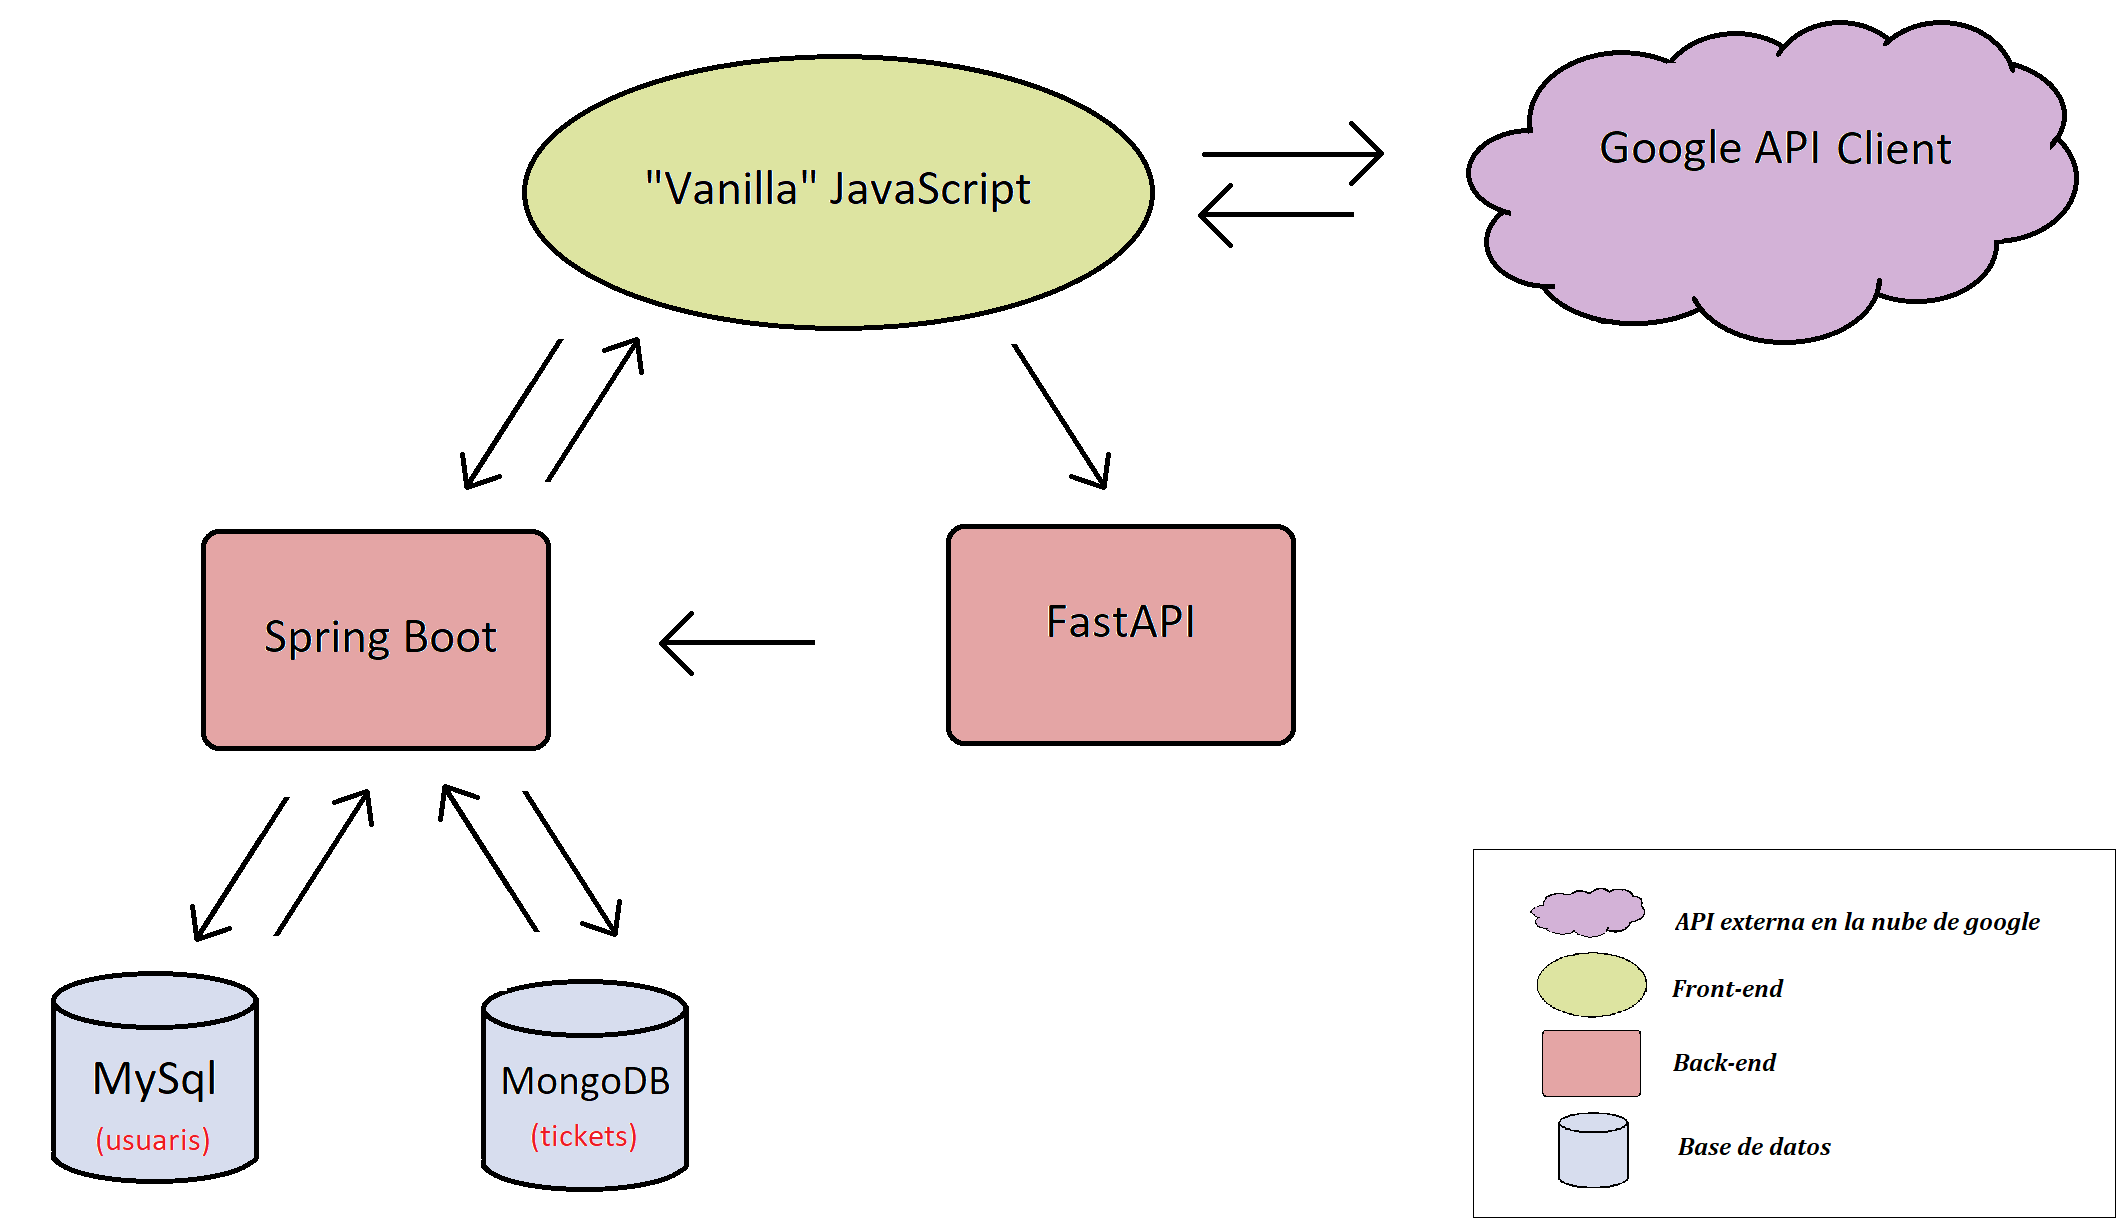
\includegraphics[width=1\textwidth]{img/diagramaSistemesAplicacioMercapp.png}
			\caption{Diagrama de sistemas simplificado de la aplicación mercApp. Tenemos el back-end de Spring Boot, donde se mandan a guardar y leer de mySQL los datos de los usuarios y gracias al cual se gestiona el enrutamiento de vistas públicas. Tenemos también el back-end de fastAPI, que parsea los tickets digitales y los pasa a formato estructurado JSON para persistirlos en MongoDB. También hacemos uso de Google API Client, que pertenece a \textit{Google Cloud}, y que permite la extracción de tickets del Gmail del usuario hacia su ordenador, a petición suya a través del navegador. El front-end con ``Vanilla'' JavaScript muestra las vistas al usuario en función del token de acceso que expide Spring Boot.}

			
			\label{fig:diagramaSistemesAplicacioMercapp} 
		\end{figure}
		\FloatBarrier
				
				
			\subsection{Camino recorrido durante el registro de usuario}
				
				
				\setlength{\belowcaptionskip}{3pt}
				\FloatBarrier
				\begin{figure}[H]
					\centering
					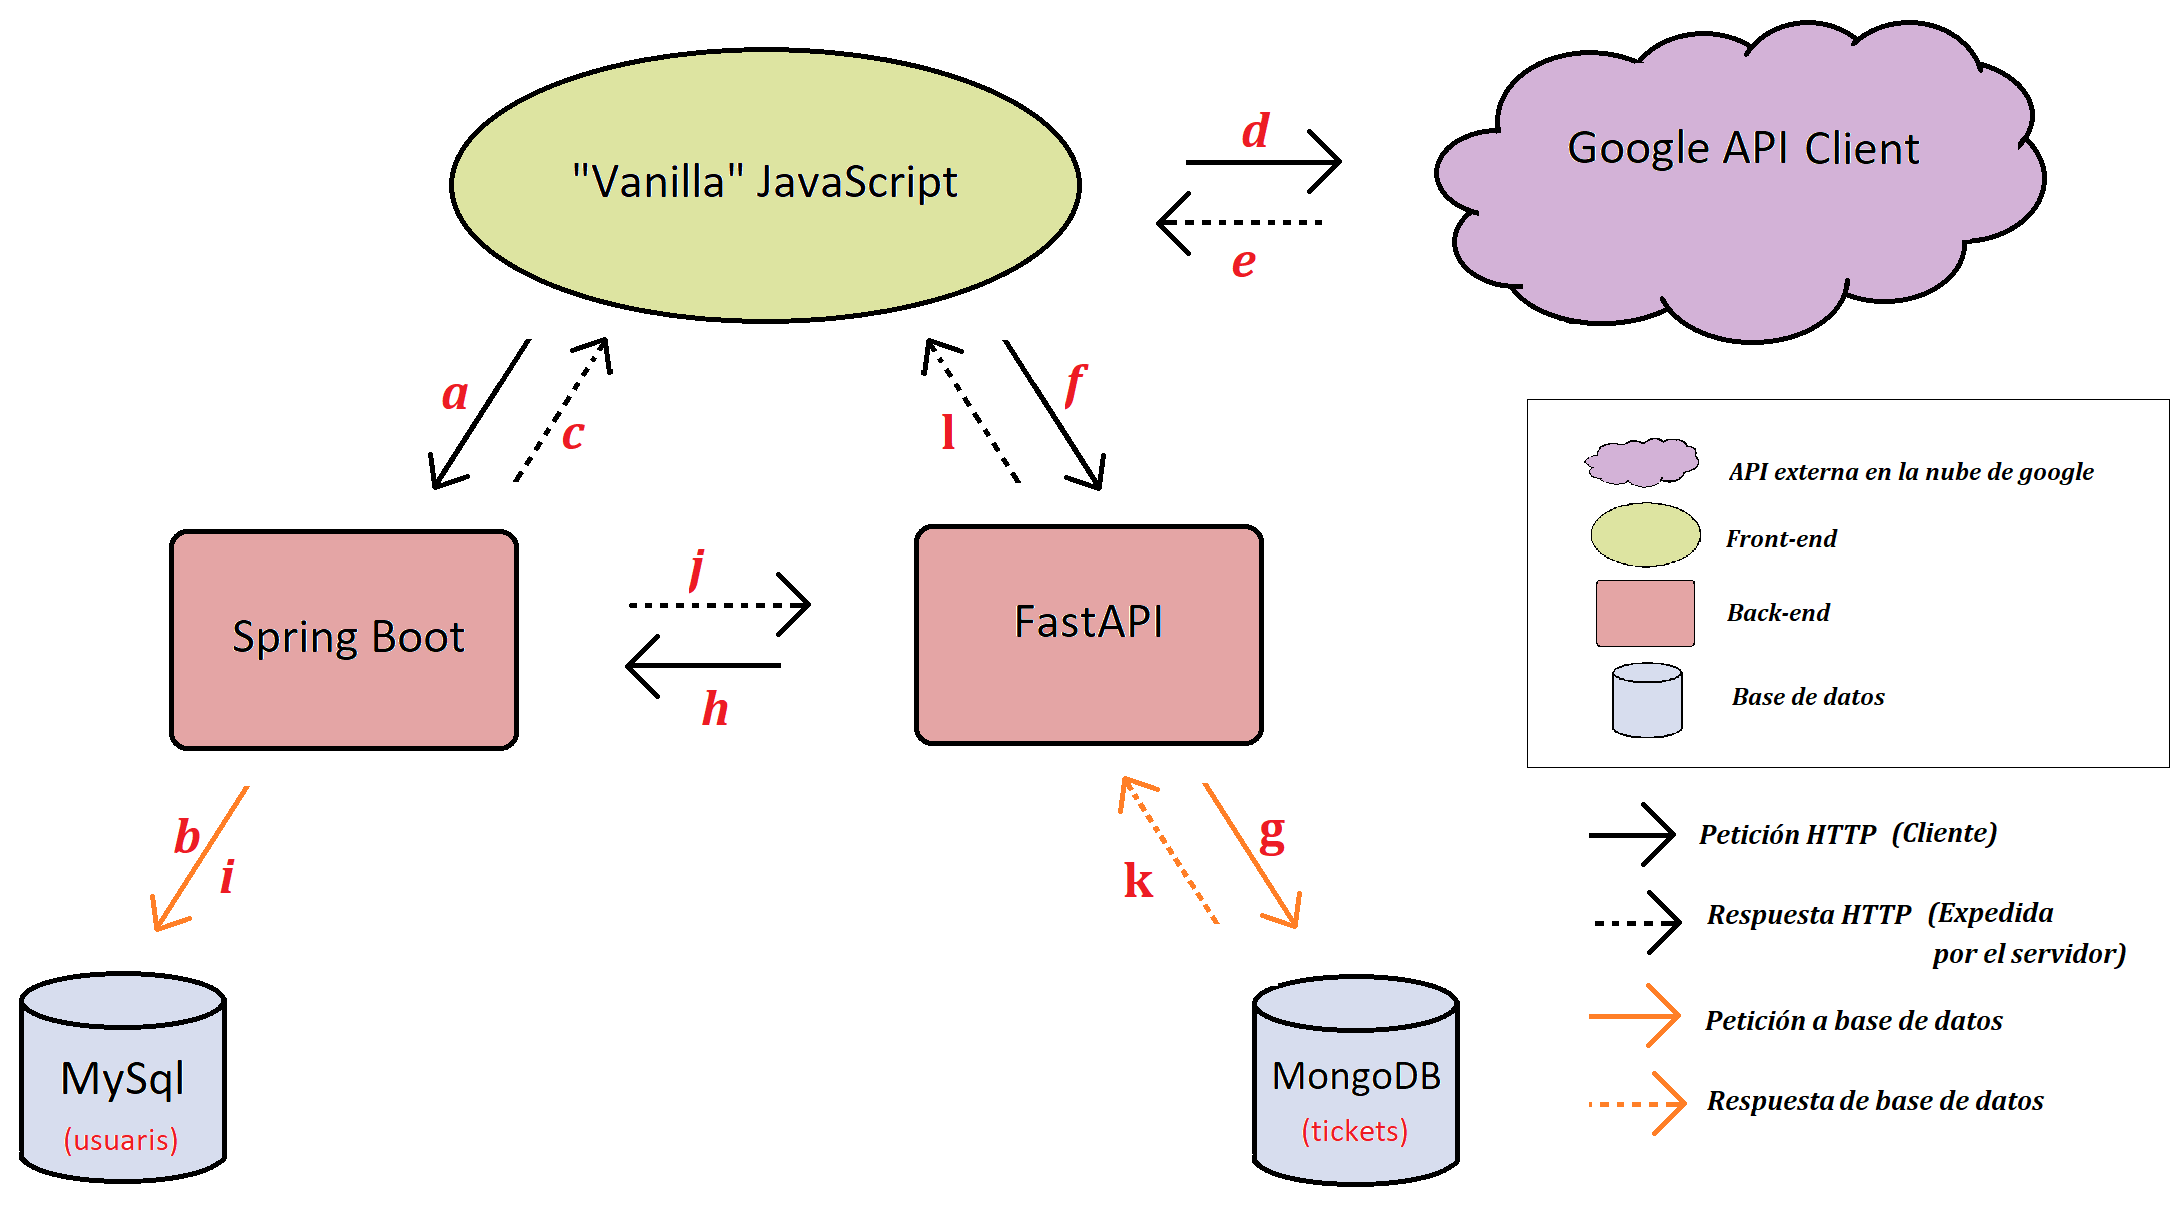
\includegraphics[width=1\textwidth]{img/diagramaSistemesAplicacioMercappCAMIREGISTREbo.png}
					\caption{Diagrama de sistemas simplificado con los caminos activados durante el registro de un usuario (no superusuario). Mostramos acontecimientos en orden desde que este introduce su correo electrónico y su contraseña por primera vez hasta que este tiene acceso al dashboard de visualización, siempre que haya éxito en todas las partes del proceso: a) Usuario pone correo y contraseña. b) guardamos correo y hash de la contraseña. c) Mandamos al front-end un token de acceso con permisos = 0 y le pedimos al usuario que nos conceda acceso a sus tickets digitales. d) usuario se autentica con la Gmail API de google API Client, con OAuth2, y automáticamente se pide la descarga de sus tickets digitales e) tickets digitales en PDF regresan al navegador y se descargan al ordenador del usuario. f) cuando el usuario lo quiera sube a fastAPI los tickets de su ordenador para que el servidor los parsee a formato estructurado g) Los tickets con formato estructurado se guardan en MongoDB h) FastAPI pasa el token de acceso con permisos = 0 hacia Spring Boot y le pide uno con permisos = 1. i) Spring Boot guarda permisos a 1 a la BBDD mySQL j) Spring Boot regresa a fastAPI el token de acceso recién expedido con permisos = 1. k) FastAPI obtiene los datos de los tickets de usuario de MongoDB l) FastAPI manda el token de acceso con permisos = 1 y los datos extraídos de MongoDB (información de los tickets) de vuelta al front-end para que JavaScript los muestre automáticamente en el dashboard de visualización.}
					\label{fig:diagramaSistemesAplicacioMercappCAMIREGISTRE} 
				\end{figure}
				\FloatBarrier
				
				
		\subsection{Camino recorrido durante el inicio de sesión}
		


		\setlength{\belowcaptionskip}{3pt}
		\FloatBarrier
		\begin{figure}[H]
			\centering
			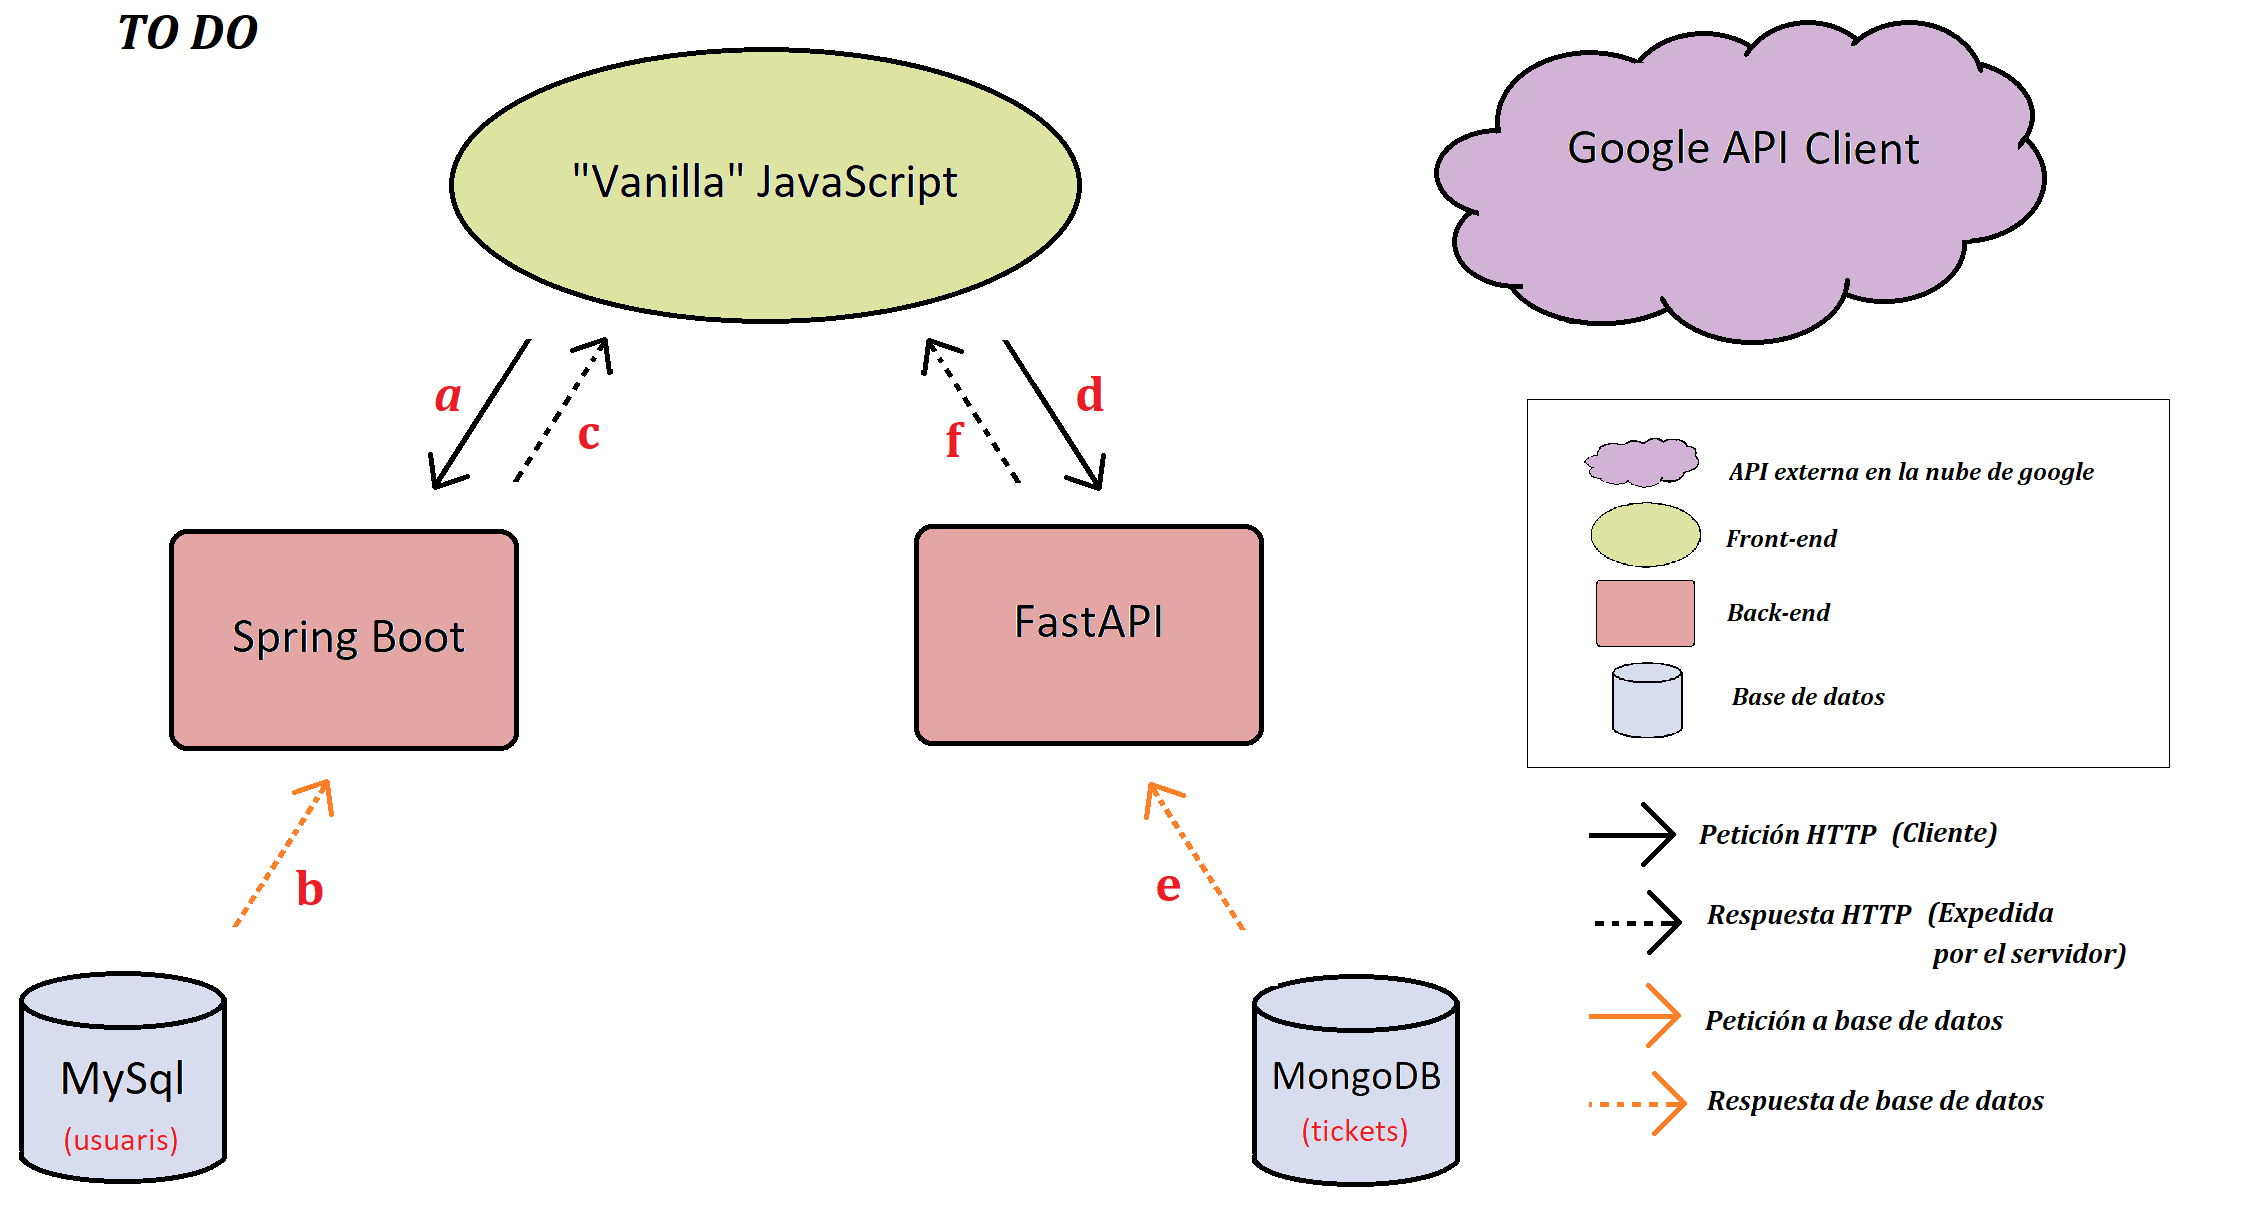
\includegraphics[width=1\textwidth]{img/diagramaSistemesAplicacioMercappCAMIINICISESSIO.png}
			\caption{Diagrama de sistemas simplificado con los caminos activados durante el \textit{inicio de sesión} de un usuario (no superusuario) que ya fue registrado, ya facilitó sus tickets digitales para su extracción o minado -parseo- y estos ya fueron extraídos y persistidos en MongoDB. Mostramos acontecimientos en orden desde que este introduce su correo electrónico y su contraseña hasta que visualiza el dashboard, siempre que haya éxito en todas las partes del proceso: a) Usuario escribe y manda correo y contraseña. b) Obtenemos usuario y hash de la BBDD y en Spring Boot vemos que son coincidentes con los que escribió el usuario por el front-end. c) Mandamos al front-end el token de acceso con permisos a 1 y automáticamente el front redirigirá a \textit{dashboard}. d) Se pide a FastAPI la información de los tickets. e) Se toman los tickets de la bbdd mongoDB. f) Se mandan de fastAPI al front-end (cliente, navegador) los datos de los tickets para ser visualizados en el dashboard.}
			\label{fig:diagramaSistemesAplicacioMercappCAMIINICISESSIO} 
		\end{figure}
		\FloatBarrier
		








		
	\pagebreak
	\chapter{Desarrollo del proyecto} %OBLIGAT
	

	
	
				
			\section{GitHub del proyecto}
			
				Para desarrollar este proyecto se ha trabajado con GitHub y git. Para su desarrollo se ha seguido la estrategia de crear ramas de característica (puede verse anexo \ref{sec:anexoFlujoGit} para ver el flujo de trabajo habitual) y, una vez satisfactoria, hacer un merge en la rama main en local. Los cambios de la rama main local se han ido subiendo al repo remoto en la rama main.
				
				Las instrucciones para correr los componentes del proyecto en sus respectivos entornos de desarrollo están en el apartado \ref{sec:entornosDesarrollo}. Las instrucciones para hacer un despliegue de la aplicación mediante contenedores Docker se encuentran en el apartado \ref{sec:despliegue}.
			

			
			
			
			
				\textbf{Link al repositorio} $\rightarrow$ \href{https://github.com/blackcub3s/mercApp}{https://github.com/blackcub3s/mercApp} 
			
	
	
		
			\section{Entornos de desarrollo}
			\label{sec:entornosDesarrollo}
			
				Para el back-end de Java con SpringBoot se ha utilizado el editor Java \texttt{IntelliJ Idea community edition} que expone el backend en el puerto \textbf{8080}\footnote{NOTA¡Para correr el proyecto back-end con\textit{Spring Boot} abrir con intelliJ la carpeta app!}: se han utilizado algunas extensiones del editor para correr el proyecto. Por ejemplo, es necesario la extensión para Lombok: sin ella IntelliJ no encontrará getters o setters y fallará.
				
				Para el front-end (archivos estáticos: HTML, CSS y JavaScript) se ha utilizado \texttt{VScode}, con la extensión live server para poder hacer llamadas al back-end directamente desde el puerto \textbf{5500}\footnote{¡El proyecto \textit{front end} con \textit{vanilla javascript} debe abrirse con vscode en la carpeta \textbf{app} y ejecutarlo en live server, si no \textbf{no} funcionará correctamente!}.
				
				Para el back-end de Python con FastAPI se ha utilizado el servidor embedido en el propio framework, expuesto en el puerto \textbf{8000}\footnote{Se recomienda ejecutarlo desde la carpeta \textit{/app} mediante \textit{fastApi dev controlador.py}} .
				
				Para la base de datos mySQL se usó workbench y se expuso el puerto \textbf{3306}\footnote{Es la versión MySQL 8.4.4 la que expone el puerto}. Para MongoDB se usó MongoDB compass exponiendo en el \textbf{27017}\footnote{Es MongoDB Community Server el que expone el puerto.}.
		
	
			\section{Despliegue}
			\label{sec:despliegue}
				Los componentes del apartado \ref{sec:entornosDesarrollo} de entornos  desarrollo se han \textit{dockerizado} de modo que cada uno de ellos sea un microservicio, a excepción (por ahora), de las bases de datos. Hemos sido cuidadosos de que los microservicios en Docker corran en los mismos puertos que los servidores embedidos con los que hemos hecho el desarrollo de la aplicación mercApp: por claridad y porque múltiples archivos dependen ya de ellos.
				
				Para crear la imagen de cada microservicio hemos creado un Dockerfile. Luego, para crear los contenedores y crear de nuevo las imágenes en caso que haya cambios en los archivos, para cada uno de estos microservicios, hay un script denominado \textit{creaImatge\_i\_arrancaContenidor.sh}\footnote{La explicación pormenorizada de sus comandos, para el caso de FastAPI por ejemplo, puede verse en el apartado \ref{sec:conteneritzacioPython}.} que reunirá todos los subcomandos de docker necesarios para el ciclo de vida de la creación de imagen (build) y subsecuente instanciado de contenedor (create, start, stop, rm). Todo ello haciendo solamente desde la terminal de Linux o desde la terminal de git bash en Windows: 
				
				\begin{lstlisting}[language=bash]
	bash creaImatge_i_arrancaContenidor.sh
				\end{lstlisting}
				
				
				
				
				
				Así, no tenemos que preocuparnos de parar un contenedor activo, borrarlo y luego crear de nuevo la imagen del que deriva (ver figura \ref{fig:dockeritzacioAplicacioPlantilla})\footnote{ A futuro planteamos hacer el despliegue con un sistema de orquestración de contenedores como es Kubernetes, subiendo las imágenes a un registry; por ahora no lo haremos y quien quiera desplegarlo en su ordenador para probarlo puede hacerlo fácilmente creando las imágenes e instanciando los contenedores con los scripts en Bash en rojo. No se hará porque las barras bajas de los nombres de las carpetas probablemente darán problemas: la memoria tiene ya muchos links al GitHub que dependen que estas rutas estén bien y por ahora no se tocará.}.
				
				
				\FloatBarrier
				\setlength{\belowcaptionskip}{3pt}
				\begin{figure}[H]
					\centering
					\caption{En rojo los archivos que crean una imagen y arrancan su contenedor, para cada microservicio. NOTA: Importante correr el script en bash con la terminal en el \textit{mismo nivel} del árbol de directorios al que pertenece el Dockerfile.}
					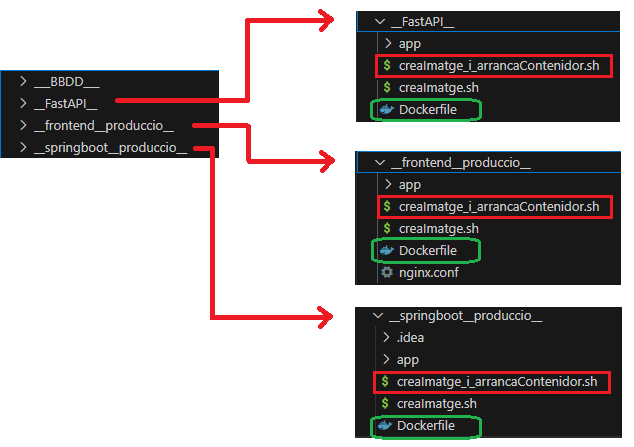
\includegraphics[width=.7\linewidth]{img/dockeritzacioAplicacioPlantilla.png}
					\label{fig:dockeritzacioAplicacioPlantilla}
				\end{figure}
				\FloatBarrier
				
			

			
			\section{Desarrollo back-end (Spring Boot, Java)}
			\label{sec:parteSpringBoot}
			
				\subsection{Contenerización}
				
				El archivo Dockerfile y los scripts en Bash para la creación de imágenes y contenedores se encontrarán \footnote{En el momento de escribir esta memoria el Dockerfile para el microservicio de Java había que programarlo. Si todavía no está disponible en el link proporcionado el lector puede dirigirse a los apartados Contenerización de los demás microservicios: FastAPI y Nginx (front-end).} \href{https://github.com/blackcub3s/mercApp/tree/main/APP%20WEB/__springboot__produccio__}{aquí}. Estos archivos se ubican, igual que lo que pasa con los demás microservicios del proyecto mostrados en la figura \ref{fig:dockeritzacioAplicacioPlantilla}, un nivel por encima de la carpeta \textit{/app}. Si el lector quiere profundizar en el tema de generar imágenes y contenedores con bash puede ir directamente al apartado \ref{sec:conteneritzacioPython} donde se explica la contenerización mediante el caso particular del microservicio de FastAPI.
			
				\subsection{Estructura de la aplicación}
				\label{sec:estructuraAplicacion}
				
				La parte de mercApp programada con Java (Spring Boot) se puede ver en el repositorio de GitHub del proyecto abriendo esta carpeta: \href{https://github.com/blackcub3s/mercApp/tree/main/APP%20WEB/__springboot__produccio__/app}{link}. Recomendamos al lector que abra y corra el proyecto con IntelliJ abriendo esta misma carpeta enlazada en GitHub, pero en local. Al hacerlo, el lector podrá ver entonces en el explorador de directorios de IntelliJ \textit{tres} rutas importantes, que son las que se encuentran por defecto en cualquier proyecto Spring Boot:
				
				\vspace{-.9em}
				\begin{itemize}
					\setlength{\itemsep}{-.5em}
					\item \textbf{src/main/java} $\rightarrow$ En esta ruta encontramos los \textit{packages} y las clases del proyecto (ver figura \ref{fig:estrucutraAplicacioJAVARESOURCES} recuadro en \textcolor{red}{rojo}).
					\item \textbf{src/main/resources} $\rightarrow$ Dentro de esta carpeta  nos encontramos con el archivo \texttt{application.properties}. Se trata de un archivo de configuración donde se define, por ejemplo, el conexionado con la base de datos (ver figura \ref{fig:estrucutraAplicacioJAVARESOURCES} recuadro en \textcolor{green}{verde}) o el archivo \textit{logback-spring.xml} que, aunque no está definido por defecto en una aplicación Spring Boot, si lo añadimos nos guarda los logs del proyecto en \textit{logs/spring.log} en lugar de salir impresos por la terminal\footnote{La ruta se crea automáticamente}. Aquí aparece como un \textit{.txt} en lugar de un \textit{.xml} porque por ahora no queremos que se guarden los errores.
					\item \textbf{pom.xml} $\rightarrow$ Es un arhivo donde encontramos el árbol de dependencias de Maven\footnote{Maven es una herramienta de automatización para la construcción de proyectos Java. Gestiona todas las dependencias, que se descargan desde un repositorio central muy vivo donde hay millones de nuevos paquetes publicados anualmente (\href{https://mvnrepository.com/repos/central}{ver link}). Maven permite empaquetar el proyecto en un .jar o .war fácilmente, entre otras cosas.} (ver figura \ref{fig:estrucutraAplicacioJAVARESOURCES}, recuadro en \textcolor{blue}{azul}): cada vez que añadimos una dependencia estamos añadiendo nuevas funcionalidades a nuestro proyecto SpringBoot a través de una descarga automatizada del repositorio central de Maven.
					
					
				\end{itemize}
				
				
				\setlength{\belowcaptionskip}{3pt}
				\FloatBarrier
				\begin{figure}[H]
					\centering
					\caption{Estructura del back-end de Spring Boot en la aplicación mercApp. \\ {\footnotesize (Cajas de color $\rightarrow$ $\{$\textcolor{red}{clases del proyecto}, \textcolor{green}{archivos de configuración}, \textcolor{blue}{dependencias de Maven}$\}$) }}
					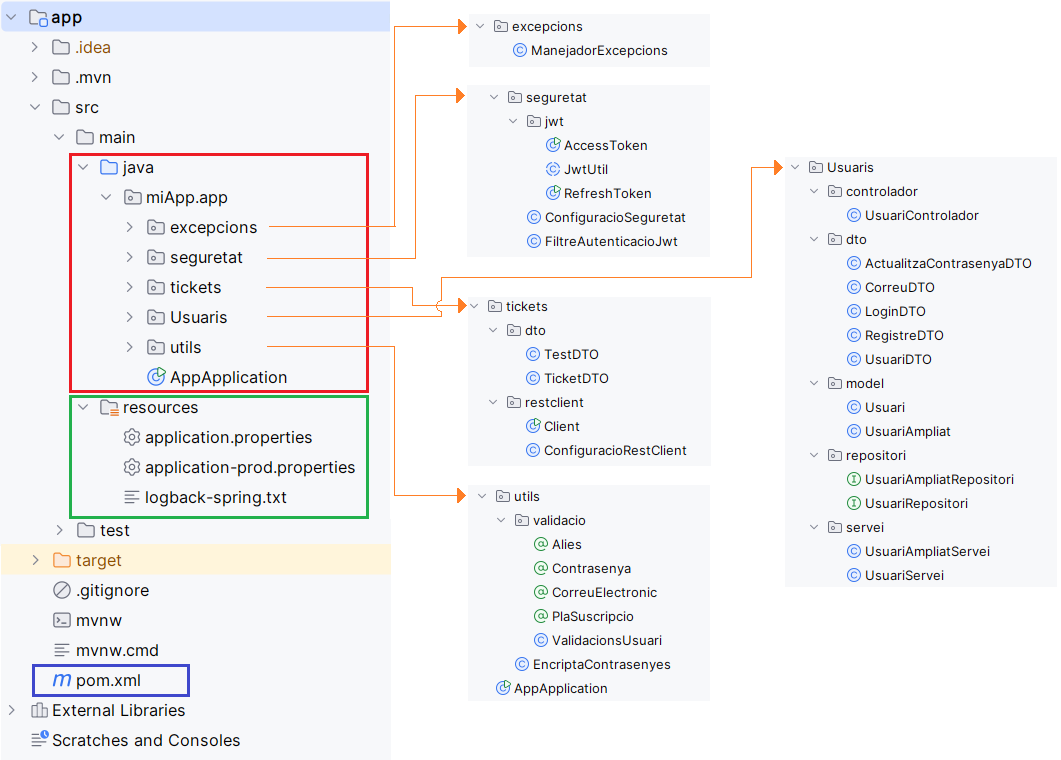
\includegraphics[width=1\textwidth]{img/estrucutraAplicacioJAVARESOURCES_final_rallat.png}
					
					\label{fig:estrucutraAplicacioJAVARESOURCES} 
				\end{figure}
				\FloatBarrier
				
				

				

				\subsubsection{src/main/java: las clases del proyecto}
				\label{sec:classesProjecteSpringboot}
				
				Dentro de \textbf{src/main/java} tenemos la ruta \textbf{miApp.app/utils/validacio}	donde residen las clases de anotación utilizadas para permitir que los campos de formulario de entrada se validen en el back-end (nótese que, con esto, hemos establecido redundancia de validaciones por si se diese el caso que un usuario maliciosamente intentase hacer llamadas directas a la API, esquivando así las validaciones ya definidas en el front-end): los archivos y su explicación quedan referenciados en detalle en el apartado \ref{sec:validacioDadesBACK}.
				
				
				
				Dentro de \textbf{src/main/java} tenemos también la ruta \textbf{miApp.app/seguretat/jwt} donde tenemos clases que generan tokens de acceso y de refresco  a partir de una clave secreta que solo está en el servidor, que referenciamos en detalle dentro de \ref{sec:implementacionJWTjava}; Análogamente, las clases que permiten implementar la autenticación y la autorización a partir de los tokens generados por las clases anteriores, las referenciamos también en detalle dentro de \ref{sec:classesSecuritzacioClaimsIfirma}.
				
				Dentro de \textbf{src/main/java} tenemos también la ruta \textbf{miApp.app/seguretat} encontramos la clase \textit{EncriptaContrasenyes.java}, que utilizamos en el servicio de usuaris para hashear las contraseñas en la base de datos. Esto lo explicamos en detalle dentro de \ref{sec:implementacioHashContra}.
				
				Dentro de \textbf{src/main/java} tenemos también la ruta \textbf{miApp.app/tickets/}. Ahí dentro tenemos unas clases diseñadas para expansiones futuras que no han sido utilizadas por ahora: por ejemplo, dentro del package \textit{restclient} tenemos una clase habilitada que permite hacer llamadas HTTP como cliente hacia el back-end de FastAPI\footnote{Ambos back-ends sí se comunicarán, pero la comunicación se establecerá finalmente en sentido opuesto: desde el back-end de Python FastAPI \textbf{hacia} el back-end de Spring Boot para que este último emita tokens, como ya explicaremos en la \textit{parte 4} del apartado \ref{sec:solicitudDeExtraccion} dedicado a FastAPI.} (sí, el back-end de Java Spring Boot puede actuar como cliente hacia otro back-end mediante la librería RestClient) . 
				
				
				Dentro de \textbf{src/main/java} tenemos la ruta \textbf{miApp.app/Usuaris} con varios subpackages. Ahí dentro merece la pena mencionar que tenemos todas las clases con las que se recibe y procesa datos del cliente para hacer la gestión de usuarios. Las que nos interesan son las siguientes:
				\href{https://github.com/blackcub3s/mercApp/blob/main/APP%20WEB/__springboot__produccio__/app/src/main/java/miApp/app/Usuaris/controlador/UsuariControlador.java}{UsuariControlador.java}, 
				\href{https://github.com/blackcub3s/mercApp/blob/main/APP%20WEB/__springboot__produccio__/app/src/main/java/miApp/app/Usuaris/servei/UsuariServei.java}{UsuariServei.java}, 
				\href{https://github.com/blackcub3s/mercApp/blob/main/APP%20WEB/__springboot__produccio__/app/src/main/java/miApp/app/Usuaris/repositori/UsuariRepositori.java}{UsuariRepositori.java} y 
				\href{https://github.com/blackcub3s/mercApp/blob/main/APP%20WEB/__springboot__produccio__/app/src/main/java/miApp/app/Usuaris/model/Usuari.java}{Usuari.java}\footnote{No nos interesa por ahora hablar mucho de UsuariAmpliat.java y de UsuariAmpliatRepositori.java porque se han creado como plantilla para la expansión de datos de usuarios si a futuro seguimos desarrollando esta aplicación.}. 
				A continuación  vamos a mostrar, a modo de ejemplo, cuál es la utilidad de todas esas clases cuando hacemos una llamada a un endpoint del \textit{UsuariControlador.java} (concretamente el endpoint \href{https://github.com/blackcub3s/mercApp/blob/78c9f573613d94a9d9de6ee046aa5d6f02f0f425/APP%20WEB/__springboot__produccio__/app/src/main/java/miApp/app/Usuaris/controlador/UsuariControlador.java#L103}{/api/login}, que veremos que es el endpoint que interviene en el inicio de sesión): más adelante veremos que este endpoint cobra un papel importante en el enrutamiento front-end de la aplicación (que mostraremos exhaustivamente en \ref{fig:diagramaMercaAppFront}) y que su utilidad es crucial para la redirección a una de las dos páginas privadas.
				
				 Antes que nada, empero, mostramos una figura explicativa a nivel gráfico de lo que pasa en este proyecto Spring Boot y, en teoria, en todos: luego iremos desgranando cada componente (ver figura \ref{fig:diagramaInjeccioDependencies}). De esta figura empezamos destacando la labor del Controlador: en Spring Boot (y probablemente en otros frameworks de back-end), los \textit{endpoints} o puntos de entrada de solicitudes HTTP, van a ser definidos dentro de lo que llaman una clase ``controller'' o controlador. En este caso, la clase controlador que nos ocupa está en el archivo \href{https://github.com/blackcub3s/mercApp/blob/main/APP%20WEB/__springboot__produccio__/app/src/main/java/miApp/app/Usuaris/controlador/UsuariControlador.java}{UsuariControlador.java}. 
				
				
							
				\FloatBarrier
				\setlength{\belowcaptionskip}{3pt}
				\begin{figure}[H]
					\centering
					\caption{Inyección de dependencias en nuestro proyecto Spring Boot bajo el modelo-vista-controlador (MVC) dentro del package Usuaris. Spring Boot añade otra capa más al modelo que ya conocíamos de desarrollo web entorno servidor: el repository (repositori). En el \textit{UsuariControlador.java} están los endpoints que tienen que ver con los usuarios. Estos endpoints dependen de la capa de servicio (UsuariServei.java), que es la que implementa la lógica de negocio. La lógica de negocio depende, a su vez, de las operaciones en base de datos, que se implementan en el repositorio (UsuariRepositori.java). El ``model'' es otra capa opcional que se implementa en Java y cuya función es mapear cada atributo de una clase Java a una columna de una tabla de la base de datos}
					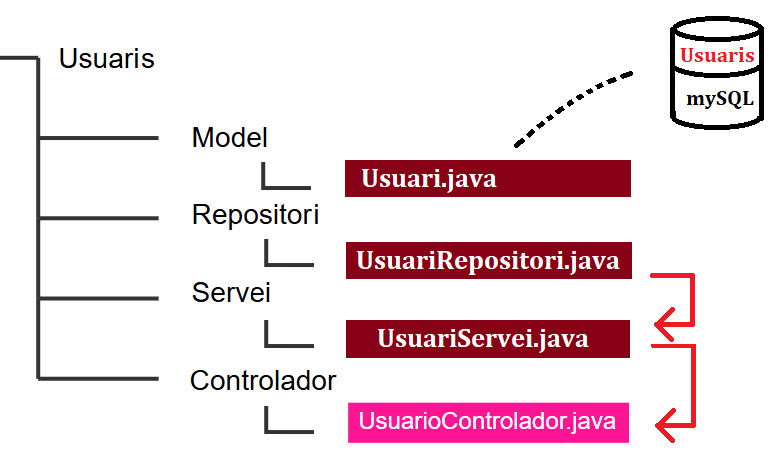
\includegraphics[width=1\linewidth]{img/diagramaInjeccioDependencies}
					\label{fig:diagramaInjeccioDependencies}
				\end{figure}
				\FloatBarrier
					
				Habiendo introducido a las clases más importantes del proyecto en la figura \ref{fig:diagramaInjeccioDependencies}, ahora, con un ejemplo, vamos a ver como estas clases interaccionan entre sí cuando un usuario llama al endpoint de inicio de sesión \textit{/api/login} con un cliente (navegador, Postman) y obtiene, como response, un JSON como el siguiente o como el que se muestra en el recuadro verde de la figura \ref{fig:apiloginspringboot}:
				
			\begin{lstlisting}[language=xml, basicstyle=\ttfamily\footnotesize, keywordstyle=\color{magenta}]
	{
	  "correuElectronic" : "acces@gmail.com", 
	  "contrasenya" : "12345678Mm\_" 
	}
			\end{lstlisting}

				
				\FloatBarrier
				\begin{figure}[H]
					\centering
					\caption{Captura de Postman: en verde la petición POST al controlador \textit{/api/login} $|$ En rojo, la respuesta de la llamada exitosa a ese controlador, resultante en la obtención de un token de acceso y otros datos.}
					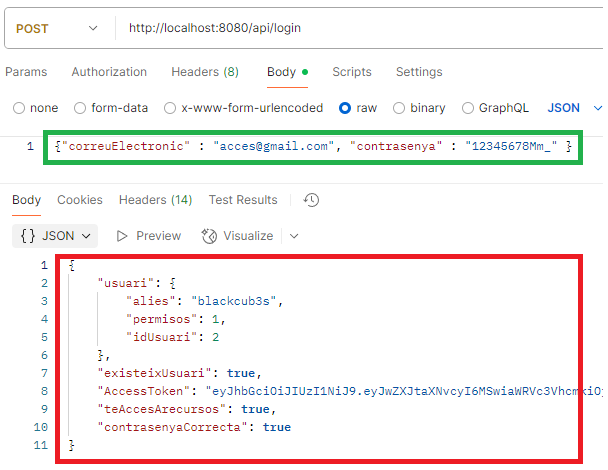
\includegraphics[width=1\linewidth]{img/apiLoginSpringBoot}

					\label{fig:apiloginspringboot}
				\end{figure}
				\FloatBarrier


.


				La petición que hace el front-end, pues, lleva el correo y la contraseña; y la respuesta que recibe este front-end o, en este caso Postman, está marcada en la figura anterior con el recuadro en rojo. Como veremos en la figura \ref{fig:esquemaArquitecturaSpringboot}, el controlador \textit{/api/login} está activado por una función denominada \textit{login} que pide obtener el body de una solicitud POST: la indicación de esperar el cuerpo o body de la solicitud se hace mediante la anotación \textit{@RequestBody} (que va a guardar el cuerpo dentro de la variable pasada por parámetro, en este caso \textit{dto}\footnote{En el apartado de validaciones hablaremos sobre los DTOs o Data Transfer Objects, y para qué sirven.}), mientras que \textit{@PostMapping} nos indica que el controlador solamente procesa solicitudes HTTP de tipo POST.
				
				Asimismo, el back-end de Spring Boot no va a permitir conexiones entrantes de un origen distinto al que está corriendo; con lo cual si queremos permitir que el endpoint del back-end \textit{/api/login} sea expuesto al front-end (que corre en un puerto distinto) necesitaremos indicarle a Spring Boot de qué lugar va a estar este front-end haciendo la petición: esto lo hacemos con la anotación \textit{@CrossOrigin}, pasándole la IP y el puerto de la aplicación front-end (5500\footnote{Esto es, básicamente, el front-end de vscode o el puerto de Nginx que hemos configurado en el Dockerfile para el despliegue en contenedores como veremos luego en el apartado \ref{sec:conteneritzacioNginx} de contenerización.}.) para que el controlador habilite conexiones entrantes desde ese origen.
				
				
				
				
				
				
				\FloatBarrier
				\setlength{\belowcaptionskip}{3pt}
				\begin{figure}[H]
					\centering
					\caption{Descripción de alguna de las funciones activadas ante un inicio de sesión que empiece por un usuario lanzando una petición POST a \textit{/api/login}. Se utilizan todas capas del modelo: controlador, servicio, repositorio y modelo (clase Usuari).}
					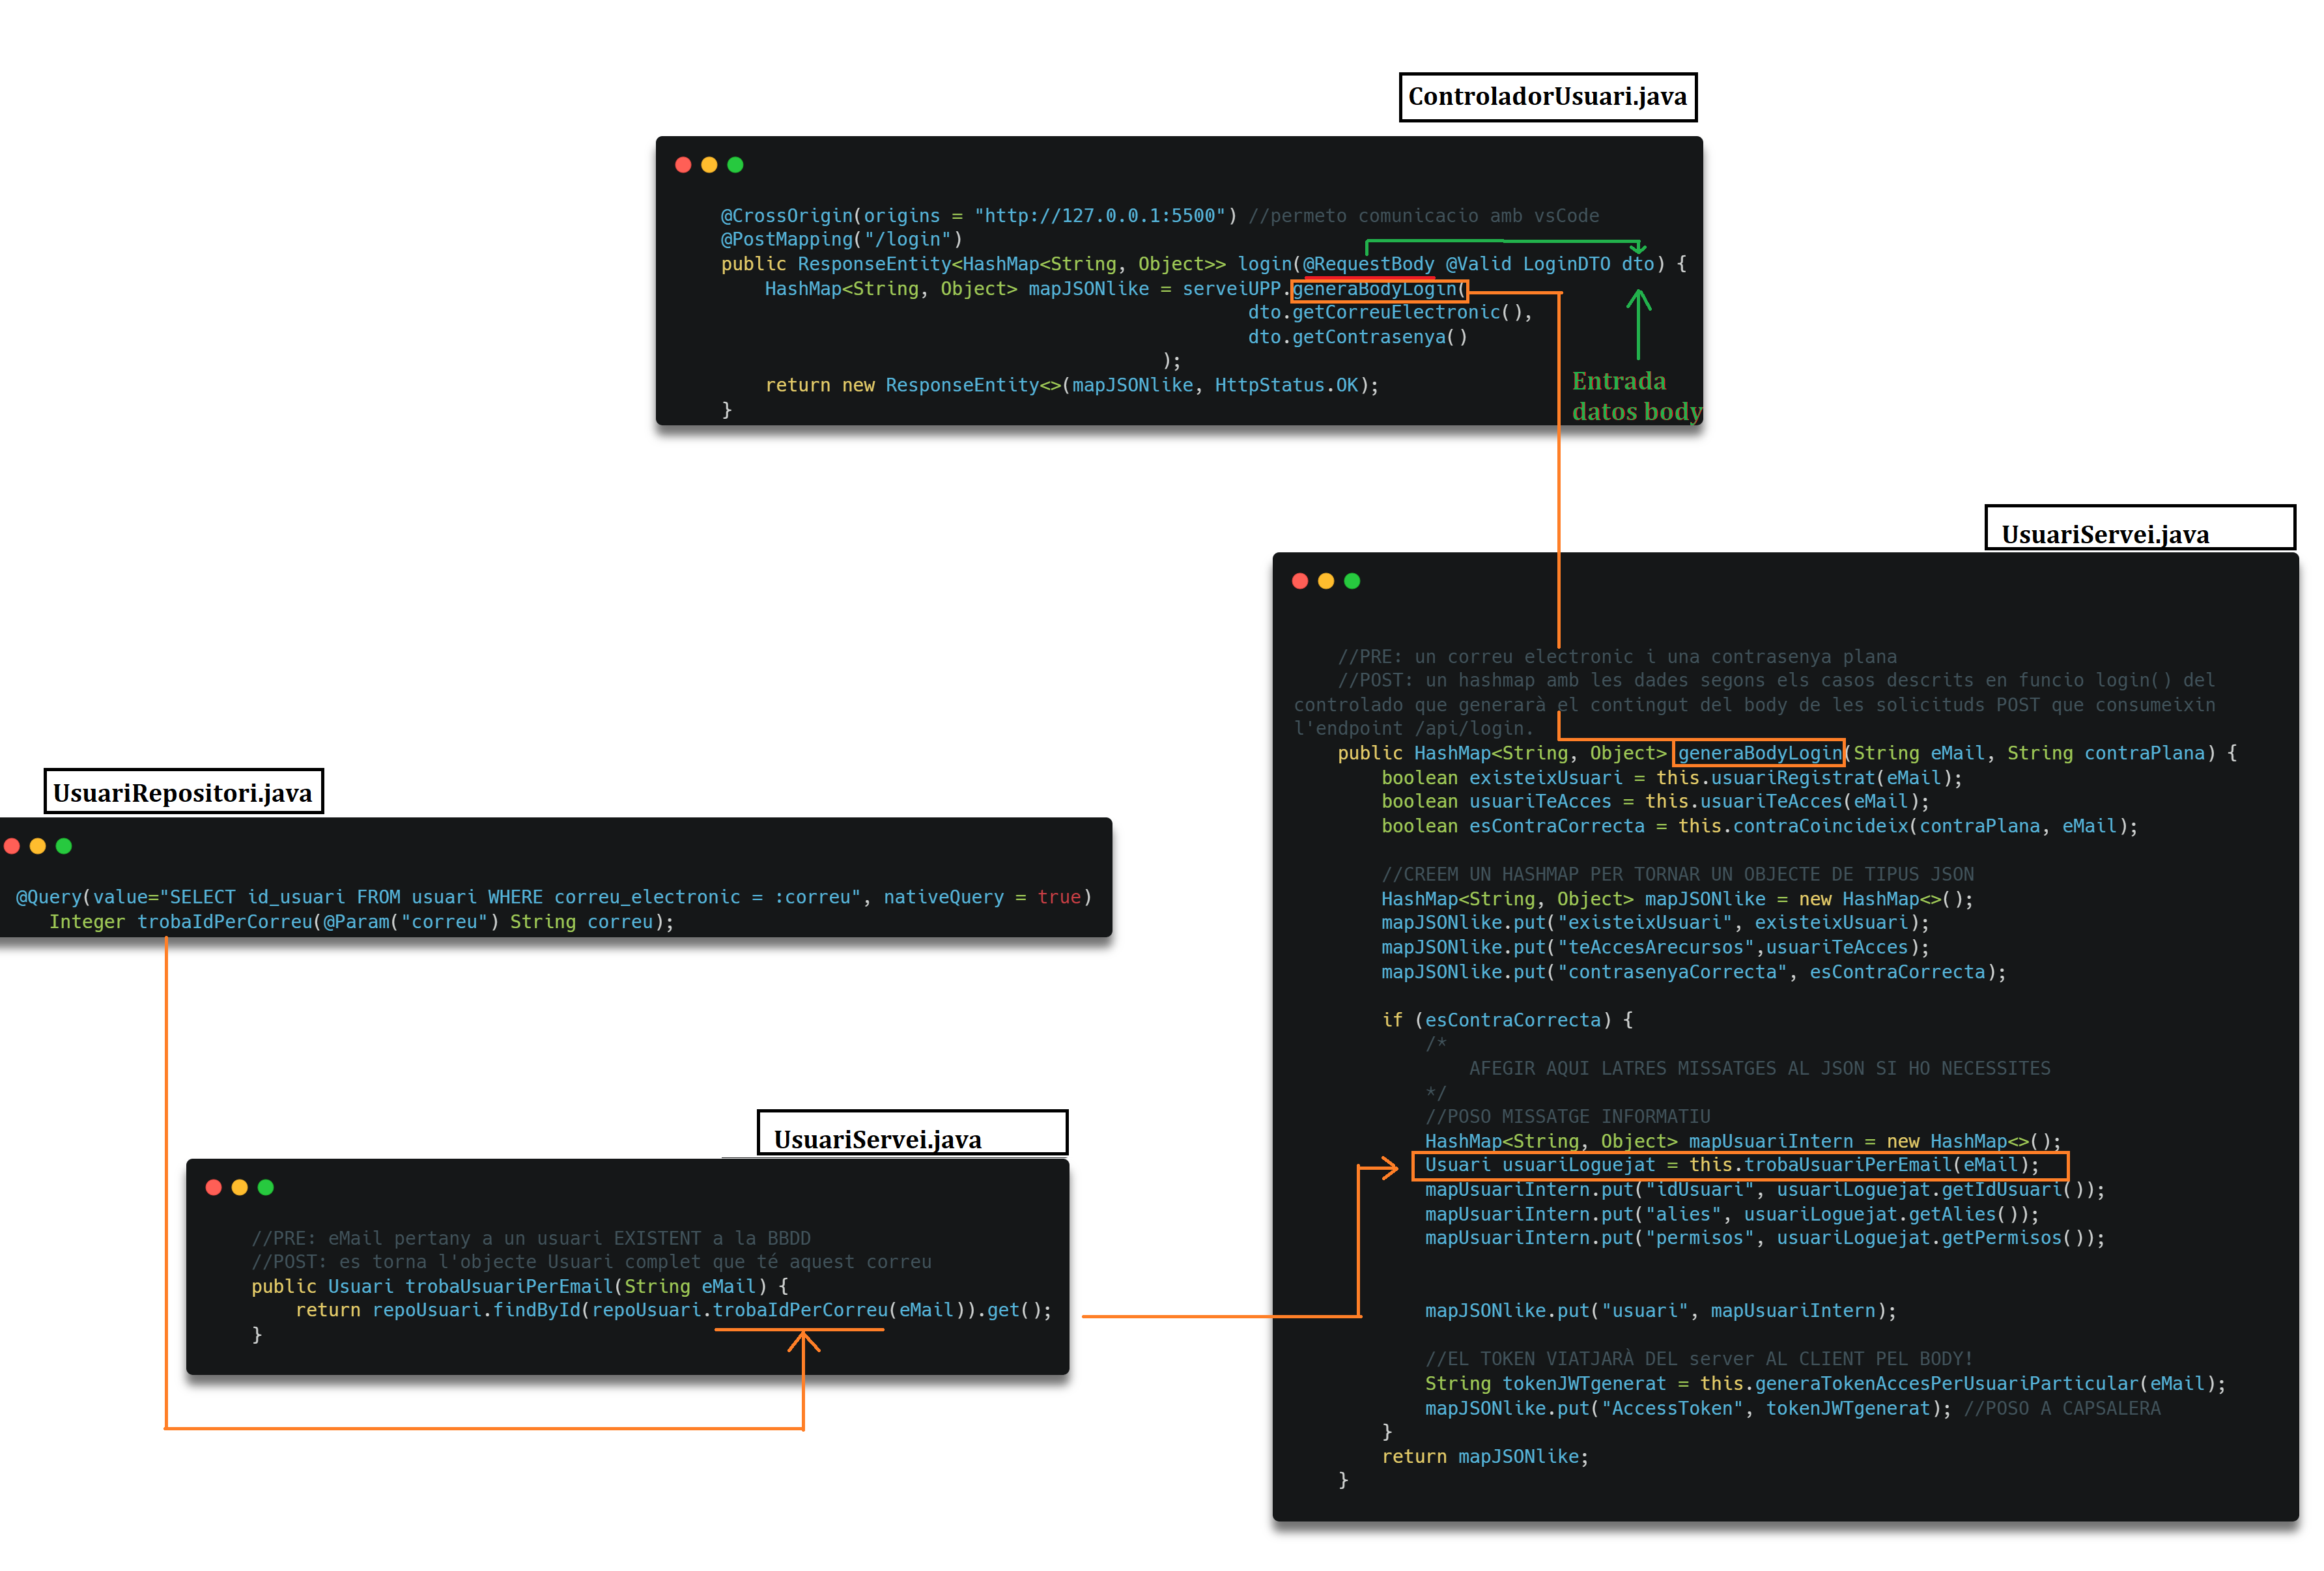
\includegraphics[width=1\linewidth]{img/esquemaArquitecturaSpringboot}
					\label{fig:esquemaArquitecturaSpringboot}
				\end{figure}
				\FloatBarrier
				
				
				Una de las partes fuertes de Spring Boot es que permite mapear objetos de la base de datos mySQL a objetos Java: esto se consigue en las clases del \textit{model}, aquellas que llevan la anotación @Entity. En nuestro caso tenemos la clase \textit{Usuari.java}, con la que podemos recoger en sus atributos una fila de la tabla Usuari de la base de datos mySQL. Esto es posible gracias a JPA (Java Persistence API), que define algo llamado ORM u \textit{Object Relational Mapping}. En teoría, si se utiliza bien el ORM ya no es necesario hacer consultas con lenguaje SQL a la base de datos porque JPA ya lleva una interfaz de la que extendemos en el UsuariRepositori.java que nos da acceso a funciones que por detrás ya implementan consultas SQL, dándonos la prerrogativa de no salir del lenguaje Java y no tener que adentrarnos en el terreno del SQL. Es por esta razón que en UsuariRepositori.java se ha definido una interfaz que hereda de  la interfaz JpaRepository. La definición de UsuariRepositori debe hacerse de forma muy específica y cuidadosa para que funcione: hay que pasarle primero el objeto con el que mapeamos la tabla mySQL (un objeto con la anotacion @Entity, de los que esté dentro del \textit{model}, en este caso Usuari y definido como en la figura \ref{fig:detallModelUsuariSBoot}) y, segundo, pasarle la clave primaria de la tabla Usuaris: \href{https://github.com/blackcub3s/mercApp/blob/69c9dffc3a959f9b19b43eaf13236ba99250878e/APP%20WEB/__springboot__produccio__/app/src/main/java/miApp/app/Usuaris/repositori/UsuariRepositori.java#L21}{ver línea de código}; en nuestro caso hemos usado funciones predefinidas como \textit{findById()}, que permiten obtener a un usuario a partir de su clave primaria desde la tabla mySQL mapeada; pero, a pesar de ello, muchas de las consultas se han definido manualmente con la anotación \textit{@Query}, como vemos en \href{https://github.com/blackcub3s/mercApp/blob/main/APP%20WEB/__springboot__produccio__/app/src/main/java/miApp/app/Usuaris/repositori/UsuariRepositori.java}{UsuariRepositori.java} en la figura \ref{fig:esquemaArquitecturaSpringboot}, porque no siempre se ha encontrado una manera de usar las funciones de JPA correctamente.
				
				A continuación, en la figura \ref{fig:detallModelUsuariSBoot} explicamos la clase \textit{Usuari.java}, perteneciente al \textit{model} de la aplicación: es indispensable definirla así para el ORM.
				
				


				\FloatBarrier
				\setlength{\belowcaptionskip}{3pt}
				\begin{figure}[H]
					\centering
					\caption{Detalle de la correspondencia existente entre objeto Java (Usuari) y entidad de base de datos (tabla usuari, mySql). $||$  \textit{@Column} nos indica en el parámetro \textit{name} el nombre exacto que tiene la columna de la base de datos a la que mapea el atributo contiguo a la anotación. $|$ @Table mapea con ORM tabla usuari con clase Usuari. $|$ @Entity habilita las anotaciones anteriores.}
					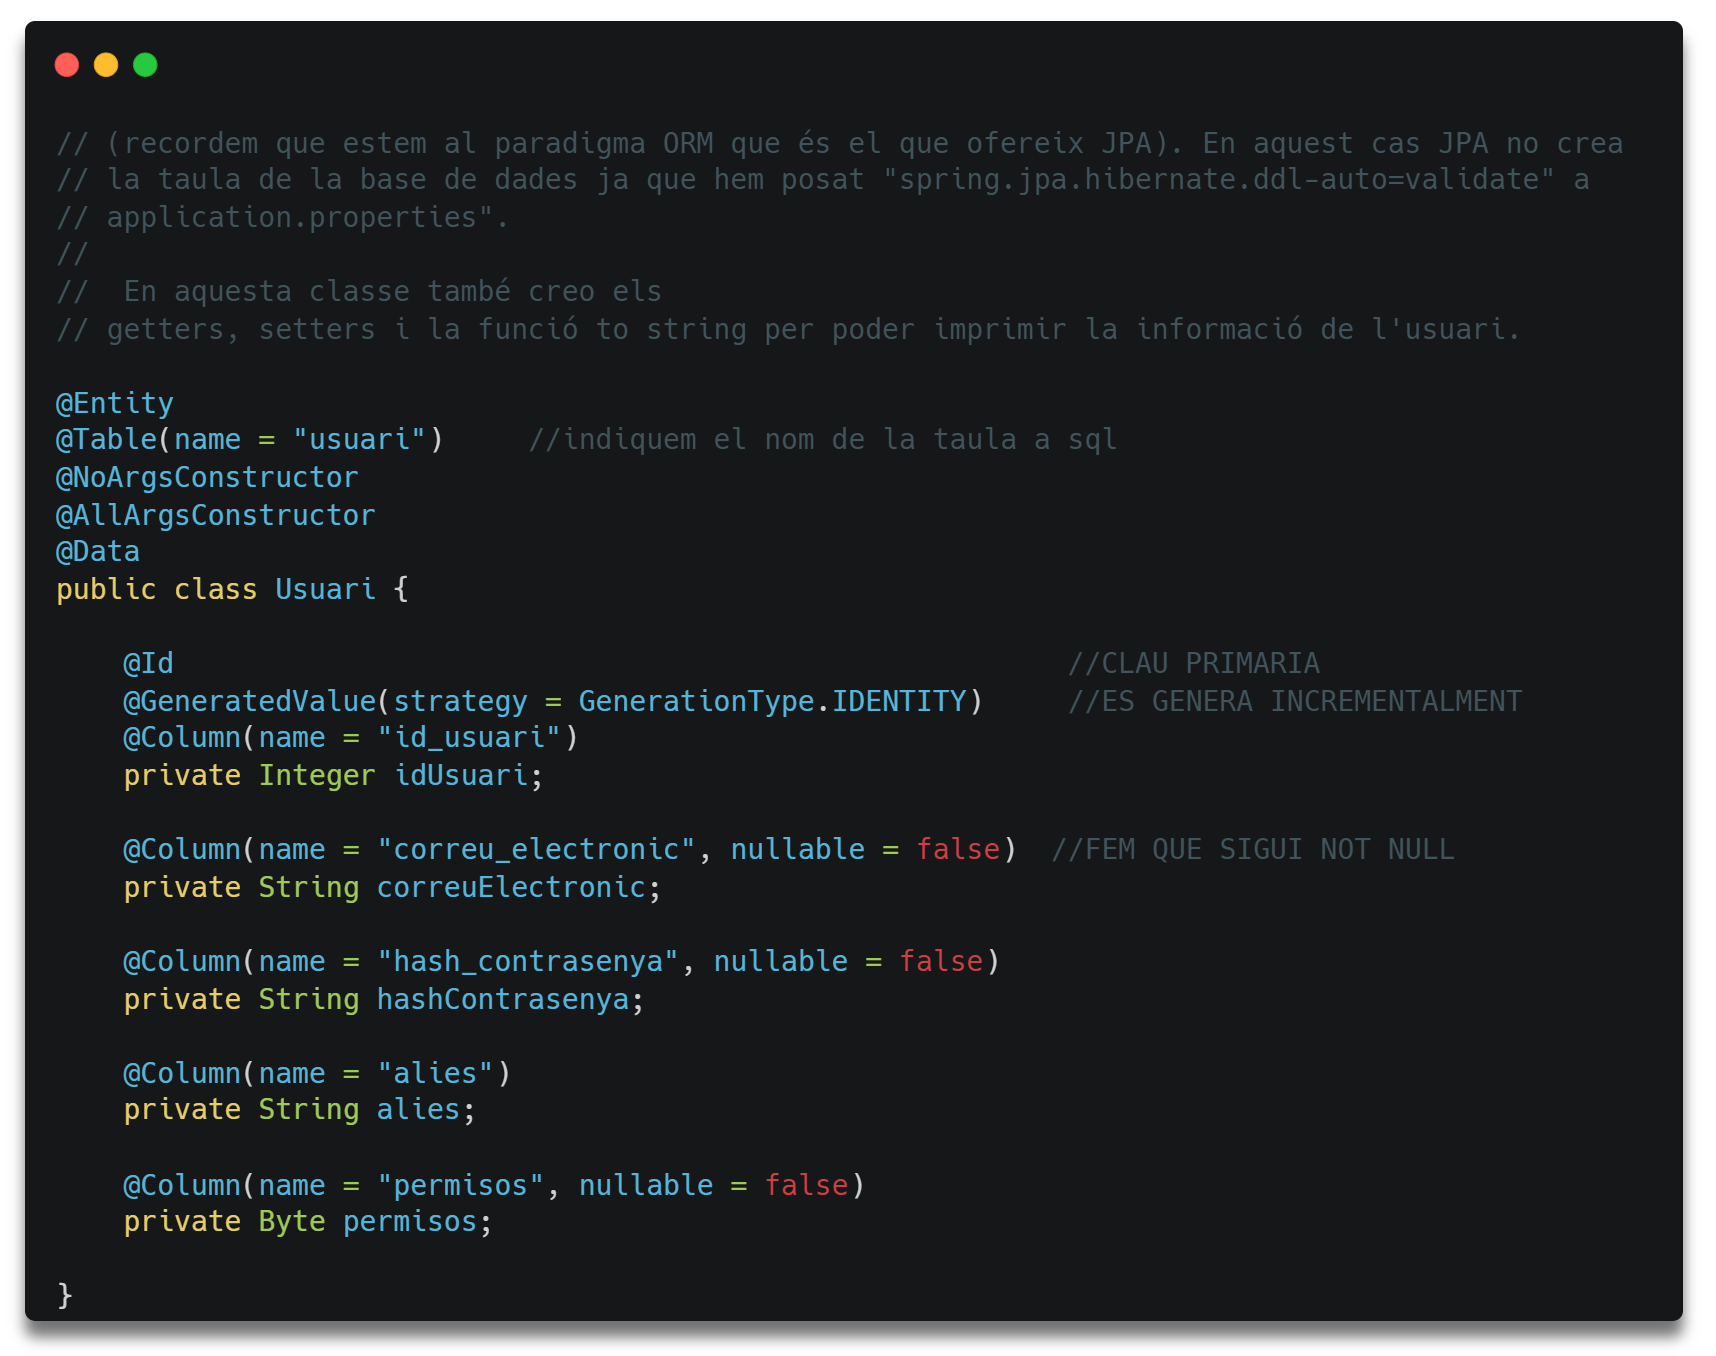
\includegraphics[width=1\linewidth]{img/detallModelUsuariSBoot}
					\label{fig:detallModelUsuariSBoot}
				\end{figure}
				\FloatBarrier
				
				Para este proyecto solamente se utilizan tres endpoints de Spring Boot en las páginas públicas (como veremos en el diagrama \ref{fig:diagramaMercaAppFront}). Sin embargo, el proyecto tiene una API REST bastante completa. Durante la realización de las prácticas en la empresa donde he estado estos tres meses y en paralelo al curso, una
				API rest completa fue creada; ésta se ha incluido también en el back-end de Spring boot aunque no se ha utilizado para el proyecto, todavía; pero podrá servir a futuro para expandir la aplicación, si se desea. Aquí un detalle de todos los controladores hechos y no utilizados, pensados para ser livianos, dejando toda la lógica de negocio en el Service y devolviendo códigos HTTP informativos ante los errores: \href{https://github.com/blackcub3s/mercApp/blob/69c9dffc3a959f9b19b43eaf13236ba99250878e/APP%20WEB/__springboot__produccio__/app/src/main/java/miApp/app/Usuaris/controlador/UsuariControlador.java#L150-L274}{link a gitHub.}
				
				
				
				
				
				\subsubsection{src/main/resources: archivos de configuración}
				
				Dentro de los archivos de configuración es necesario mencionar el archivo \href{https://github.com/blackcub3s/mercApp/blob/main/APP%20WEB/__springboot__produccio__/app/src/main/resources/application.properties}{application.properties}: en él se define la conexión a la base de datos mySQL (\href{https://github.com/blackcub3s/mercApp/blob/69c9dffc3a959f9b19b43eaf13236ba99250878e/APP%20WEB/__springboot__produccio__/app/src/main/resources/application.properties#L5-L9}{detalle líneas}), se pide que el ORM valide si las anotaciones de la clase Usuari coinciden con el DDL de la base de datos (\href{https://github.com/blackcub3s/mercApp/blob/69c9dffc3a959f9b19b43eaf13236ba99250878e/APP%20WEB/__springboot__produccio__/app/src/main/resources/application.properties#L13}{detalle líneas}) y se pide que se habilite otro perfil que va a sobrescribir las propiedades que ya estén escritas en \textit{application.properties}: por ejemplo, nosotros hemos habilitado el perfil \textit{application-\textbf{prod}.properties} con \href{https://github.com/blackcub3s/mercApp/blob/69c9dffc3a959f9b19b43eaf13236ba99250878e/APP%20WEB/__springboot__produccio__/app/src/main/resources/application.properties#L26}{esta linea}. Por lo tanto, si ahora escribimos en el mismo árbol de directorio que \textit{application.properties} otro archivo de configuración denominado \textit{application-\textbf{prod}.properties} vamos a sobreescribir en \textit{application.properties} aquellas propiedades que defina este nuevo perfil. Esto es útil, por ejemplo, para entornos de producción donde queremos cambiar la base de datos de una base de datos en un servidor y no en local.
				
				\subsubsection{pom.xml: dependencias de maven}
				
				Los proyectos java pueden correr en gradle o maven. En nuestro caso el proyecto se ha hecho con maven. En pom.xml (ver \href{https://github.com/blackcub3s/mercApp/blob/main/APP%20WEB/__springboot__produccio__/app/src/main/resources/application.properties}{aquí}) se describen todas las dependecias que tiene nuestro proyecto, conjuntamente con la versión de las mismas. Si queremos instalar una nueva dependencia en el proyecto basta con añadirla en el pom.xml y dentro de intelliJ hacemos click derecho \textit{Maven} $\rightarrow$ \textit{syncProject}. Entonces IntelliJ nos descargará las dependencias nuevas desde maven central (que es donde están todos los repositorios de Java).
				
				Por ejemplo, para poder definir JWT o JSON Web Token hemos tenido que cargar esta dependencia específica en pom.xml (podeis ver más información en el apartado \ref{sec:implementacionJWTjava}). Por ejemplo, para definir Lombok\footnote{Es una dependencia muy usada en Spring Boot, que permite generar getters y setters para una clase, pero sin que estén escritos: así si se cambia el nombre de los atributos de una clase, los getters y setters cambian también de forma automática.} hay que definir este xml y, sobretodo, incluir la versión que utiliza la dependencia, tal que así:
				
				
			\begin{lstlisting}[language=XML, basicstyle=\ttfamily\small, keywordstyle=\color{red}]
					
	<!-- fes getters i setters automatics -->
	<dependency>
		<groupId>org.projectlombok</groupId>
		<artifactId>lombok</artifactId>
		<version>1.18.36</version>
		<scope>provided</scope>
	</dependency>
			
			\end{lstlisting}
				 
				
				Para saber cuál es la versión más actualizada -o la más usada- de un plugin basta con entrar a mvnrepository.com y consultarlo. Por ejemplo, para el caso de lombok tenemos este \href{https://mvnrepository.com/artifact/org.projectlombok/lombok}{link}.
			
				
				\subsection{Autenticación y Autorización}
				
				\subsubsection{método utilizado: JWT}
				
				Para autenticar y autorizar a los usuarios no utilizaremos sesiones. Las sesiones, tal y como vimos en la asignatura de desarrollo web entorno servidor, requieren guardar un estado en el servidor (si tenemos 100 usuarios conectados necesitamos rastrear 100 personas en el servidor) y un identificador de sesión en una cookie segura con HttpOnly puesto a True guardada en el navegador de cada uno de los usuarios conectados que lo identifica en relación al servidor.
				
				Sin embargo, existe un método de acceso por token más escalable que no requiere guardar sesiones en el servidor (es decir, es un método ``stateless'' o sin estado) con el que nos basta tener solamente la Cookie Segura para guardarlo y ya está. Es un token que está autocontenido: es decir, puede contener ya el ID de usuario, nombre de usuario, roles que luego permitirán dar permisos o no en el servidor para acceder a determinadas APIs o recursos, etc. En definitiva, con JWT tenemos una autenticación más eficiente y un control del acceso preciso (autorización) sin necesidad de almacenar sesiones en el servidor.
				
				
				A este sistema lo llamamos JSON Web Token (\texttt{JWT}) y toda la información que contiene está \textbf{firmada digitalmente} con SHA256 mediante una clave privada (el ``secret'') que solo tenemos nosotros en el servidor\footnote{El token está firmado, pero no cifrado: todo el mundo puede ver su contenido.}. Esta clave es igual para todos los tokens que generemos: la firma digital que emana de esta clave estará embedida, por así decirlo, en cada uno de esos tokens y \textit{será inválida} si un atacante ha modificado el token y nos lo devuelve al servidor tratando de suplantar la identidad de algún usuario; con ello, el servidor rechazará la integridad del token y evitará que pueda acceder a recursos del usuario al que trata de suplantar.
				
				JWT no es perfecto, por supuesto. Una desventaja del JWT es que una vez puesta una fecha de expiración el desarrollador ya no la puede cambiar. En las sesiones del servidor se pueden extender las sesiones si se detecta actividad del usuario, acortarlas si pasa justo lo contrario o incluso cerrar la sesión de un usuario en remoto; pero con JWT no es posible: una vez creado el Token de acceso la fecha de actividad del mismo no se puede modificar (¡porque no puedes invalidar un token ya existente!), lo cual permite que simplemente un atacante robe el token de acceso sin modificarlo y lo use hasta su fecha de expiración.
				
				Se proponen dos soluciones posibles a este problema, ninguna de las cuales ha sido implementada en este proyecto y queda definitivamente como uno de los puntos de mejora:
				
				\begin{itemize}
					\setlength{\itemsep}{.0em}
				
					\item 1. Tener dos tokens almacenados en el cliente: el ``access token'' que es el que permite autenticar y autorizar, del que hemos hablado hasta ahora; y otro token denominado ``refresh token'', que se utiliza
					para obtener un nuevo token de acceso cuando el token de acceso actual expire, o para obtener tokens de acceso adicionales con una duración igual o más corta \cite{stackoverflow_refreshTokenAvantatjaSeguretat}
					
					\item 2. Crear una black-list de tokens de acceso donde se añadirán los usuarios que hayan hecho ``log out'' \textbf{antes} de la expiración programada de su token de acceso: así si un token de acceso todavía no expirado sabemos que su usuario se ha deslogueado, y en caso que sea robado el servidor podrá rechazar la petición no permitiendo acceso a recursos \cite{stackOverflow_blackList}) porque tendrá información de la voluntar de desloguearse por parte del usuario real.
 
					
				\end{itemize}

				
				
				En este trabajo solo utilizaremos ``access tokens'' y ya está. Cuando un usuario se desloguee, lo que haremos simplemente será borrar el access token del \textit{local storage}. Tampoco guardaremos los tokens en una cookie segura porque complica el desarrollo (de nuevo, otro punto a mejorar a futuro en este proyecto).
			
				 
				 \noindent En resumen, \texttt{las ventajas} que tiene JWT vs uso de sesiones (si asumiéramos que tanto el JWT como el SESSID se guardasen en una cookie segura, respectivamente) serían las siguientes:
				 
					\begin{tabular}{l}
						\textbf{- No depende del almacenamiento en el servidor} \\
						\textbf{- Firmado digitalmente} \\
						\textbf{- Mayor control sobre el acceso} \\
						\textbf{- Mayor descentralización} \\
						\textbf{- Menos carga para el servidor}
					\end{tabular}
									 
				   \noindent Y las \texttt{desventajas} más evidentes que tiene JWT, en nuestra opinión, son \footnote{Se puede ver una tabla de diferencias más en profunidad, especialmente en materia de seguridad en el anexo \ref{sec:anexo_JWTvsSESSIONS})}:
				  
				  \begin{tabular}{l}
					 \textbf{- Caducidad de tokens irrevocable}\\
					 \textbf{- Necesidad de manejar tokens de refresco + tokens de acceso}
				  \end{tabular}
				 

				
				
				
				\subsubsection{¿Qué compone un JWT?}
				\label{sec:queComponeJWTbackend}
				
				\noindent El JWT se compone de tres partes separadas por \textit{puntos}: \textbf{el header}, \textbf{el payload} y \textbf{la signatura}. En la página \href{https://jwt.io/}{https://jwt.io/}, como veremos después, se puede ver si los tokens son válidos, observar el contenido de su payload, etc. \cite{jwtio}. A saber:
				

				\begin{itemize}
					\setlength{\itemsep}{-.5em}
					\item 				\textbf{Los headers}: Aportan información sobre el algoritmo que lo encriptó.
					\item 				\textbf{El payload}: Es donde está la información que nos interesa del token: el sujeto que lo generó (``sub''), el momento en que se generó el toquen (``iat'', o ``issued at'') y la fecha de expiración (``exp'' o ``expiration time''). También podemos tener ahí otros pares clave valor que podremos querer definir, por ejemplo, que contengan el id del usuario y sus roles o permisos que son los que nos permitirán dejar que un determinado usuario pueda consultar o no ciertos recursos.
					
					\item \textbf{La signatura}: Es la parte que garantiza la integridad del token y evita que sea alterado por terceros. Se genera aplicando un algoritmo de hash (en nuestro caso el SHA256) a la combinación del header y el payload, junto con la clave secreta que solo conoce el servidor (es lo que permetirá al servidor rechazar el token si no es válido -i.e. ha sido manipulado).
				\end{itemize}
				
				Podéis observar estas tres partes en colores en la figura \ref{fig:jwtioMostraPayload} que veremos después.
				
				
				

				

				
				
				\subsubsection{Implementación de JWT en java SpringBoot}
				\label{sec:implementacionJWTjava}
				Para poder implementarlo añadimos la dependencia \textbf{jjwt} en \texttt{pom.xml} que es la que nos permite definirlo.
				
				
				\begin{lstlisting}[language=XML, basicstyle=\ttfamily\small, keywordstyle=\color{red}]
					
	<dependency>
		<groupId>io.jsonwebtoken</groupId>
		<artifactId>jjwt</artifactId>
		<version>0.12.6</version>
	</dependency>
					
				\end{lstlisting}
				
				
		En el proyecto se han creado tres clases dentro de sus respectivos archivos en la ruta \texttt{src/main/java/} \texttt{miApp.app/seguretat/jwt} denominadas:
		
		\begin{itemize}
			\setlength{\itemsep}{-.4em}
			\item \textbf{JwtUtil}
			\item \textbf{AccessToken}
			\item \textbf{RefreshToken}
		\end{itemize}
		  
		
		En la clase \textbf{JwtUtil} hemos creado un método que obtiene las \textit{claims} (pares clave valor que contienen la carga útil de un JWT) y en el constructor hemos creado la definición de una clave privada con la que derivar todas las instancias que hagamos de esa clase -es decir, todos los tokens que se cifren con esa contraseña-. De esta clase hemos heretado las otras dos: la subclase que nos genera el \textit{token de acceso}, \textbf{AccessToken}; y la que nos genera el \textit{token de refresco}, \textbf{RefreshToken}\footnote{La clase RefreshToken la hemos programado para usarla a futuro pero no se ha utilizado para la implementación del sistema de autenticación y autorización en este proyecto.}. A continuacion podéis, de estas tres, ver la más importante: 
		
		

		
\begin{lstlisting}[language=Java, basicstyle=\ttfamily\footnotesize, keywordstyle=\color{magenta}]
				
@Component
public class AccessToken extends JwtUtil {
	
  private static int tExpM; //minuts per a exprirar el token
	
  public AccessToken() {this.tExpM = 10;}
	
  //FINALITAT: Generar un JWT d'acces.
  public String genera(String correu, int idUsuari, byte permisos) {
	Map<String, Object> dadesExtraApayload = new HashMap<>();
	dadesExtraApayload.put("permisos", permisos);
	dadesExtraApayload.put("idUsuari", idUsuari);
		
	return Jwts.builder()
	 .setClaims(dadesExtraApayload) //dades customitzades
	 .setSubject(correu)            //guardo nom subjecte (clau "sub")
	 .setIssuedAt(new Date())       //data creacio (clau "iat" payload)
	 .setExpiration(new Date(System.currentTimeMillis() + (tExpM*60*1000)))
	 .signWith(SignatureAlgorithm.HS256, clauSecreta.getBytes())
	 .compact();
}


\end{lstlisting}
		
		
		
		Con la función \textbf{genera()} de la clase AccessToken arriba mostrada, y con los parámetros necesarios para autorizar (idUsuari) y autenticar (permisos), podemos generar un token de acceso en ``accesJWT'' que es el usado en la aplicación para permitir acceder a los endpoints o no:
		
		
		
\begin{lstlisting}[language=Java, basicstyle=\ttfamily\footnotesize, keywordstyle=\color{magenta}]

AccessToken accessToken = new AccessToken();
String accesJWT = accessToken.genera(
	"santo@gmail.com",  //campoSub
	2, //idUsuari
	1  //permisos
);


\end{lstlisting}
		
		Si vemos la figura \ref{fig:jwtioMostraPayload} que tenemos a continuación, veremos en la mitad izquierda un token de acceso generado por la función anterior. Fijémonos que internamente ese token está estructurado en las tres partes mostradas en la mitad derecha de la imagen, siendo la parte ``payload'' la más importante, porque contiene la carga útil que usaremos para autenticar y autorizar en mercApp:
		
	
			\setlength{\belowcaptionskip}{3pt}
			\FloatBarrier
			\begin{figure}[H]
				\centering
				\caption{Decodificación mediante \href{https://www.jwt.io}{jwt.io} de un token de acceso usado en nuestra aplicación generado con la función ``genera()'' de la clase AccessToken. La Payload con las claims en flecha verde.}
				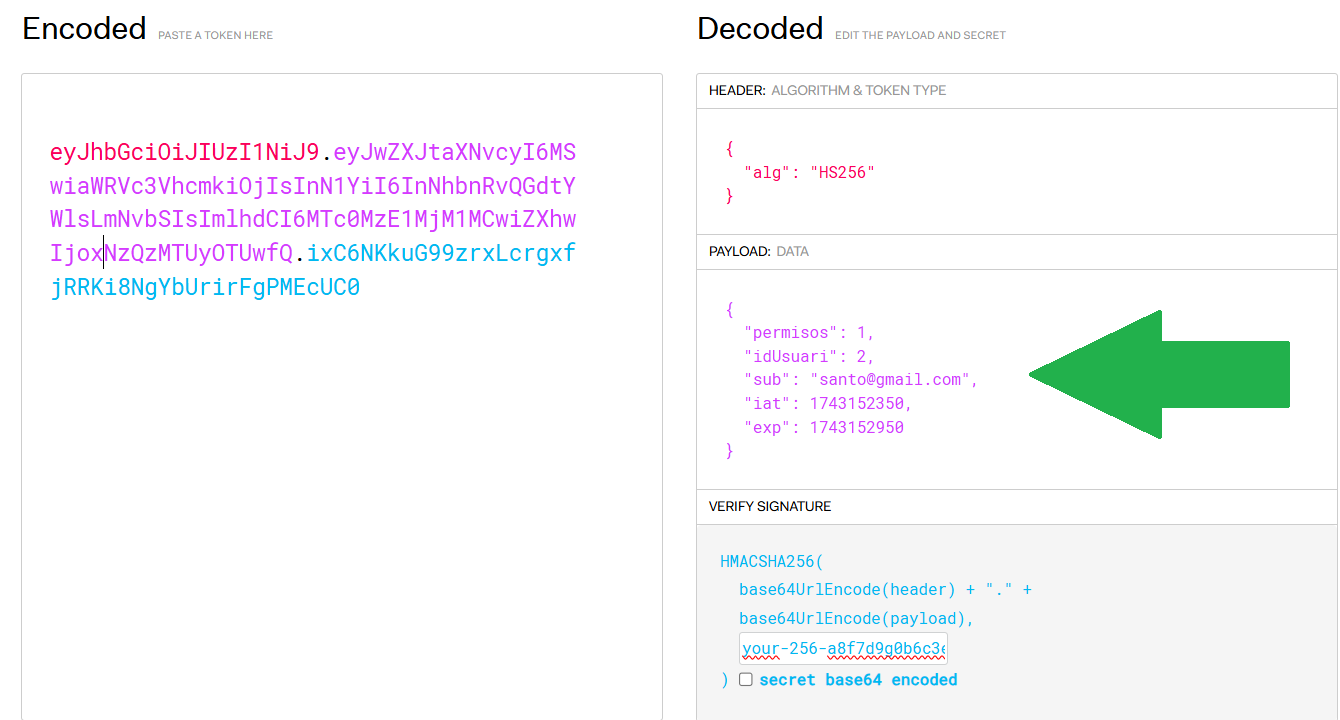
\includegraphics[width=1\textwidth]{img/jwtio_mostra_payload.png}

				\label{fig:jwtioMostraPayload} 
			\end{figure}
			\FloatBarrier

		
\begin{lstlisting}[language=Java, basicstyle=\ttfamily\footnotesize, keywordstyle=\color{magenta}]
			
		
		{
		    "permisos": 1,
		    "idUsuari": 2,
		    "sub": "santo@gmail.com",
		    "iat": 1743152350,
		    "exp": 1743152950
		}
			
\end{lstlisting}
		
		
		
		
		
		Al generar las tres clases hemos utilizado herencia porque la clave privada es la misma para ambos tipos de token (tanto el de acceso como el de refresco), mientras que los métodos para generar cada uno de los dos tipos de token cambian. En StackOverflow existe un debate para ver si hay que tener una clave privada distinta para cada tipo de token, por si el lector está interesado \cite{stackoverflow_jwt_refresh_token_secret}. Después de ver la entrada en StackOverflow se ha optado por compartir claves para ambos tipos.
		
		
		En la clase \textbf{JwtUtil} tenemos una función denominada \texttt{getClaims()} que es la que utilizaremos en el Service de nuestra aplicación para poder autenticar y autorizar usuarios. Las tres clases pueden ser consultadas en el anexo \ref{sec:anexoCreacionYverificacionJWT} o en el GitHub del proyecto (\href{https://github.com/blackcub3s/mercApp/blob/main/APP%20WEB/__springboot__produccio__/app/src/main/java/miApp/app/seguretat/jwt}{link})\footnote{Se recomienda encarecidamente al lector optar por esta última opción}\footnote{Al poner las tres clases en anexo se omitieron las funciones main donde se testeaban las funciones de creación de tokens con control de excepciones, comentarios e imports por falta de espacio en el DIN A4.}.
		
		\subsubsection{Enviar por primera vez el Access Token hacia el front-end (registro)}
		\label{sec:enviarPorPrimeraVezAccesTokenDESDEBACKEND}
		
		Cuando el usuario consigue poner la contraseña correcta en la página de registro del front-end (\texttt{pas3C\_crearContrasenya.html}), esta contraseña se manda conjuntamente con el correo electrónico\footnote{el correo electrónico  lo teníamos guardado en el localStorage de la página de registro inicial.}  mediante una petición POST al controlador de endpoint \textit{api/registraUsuari} de nuestro back-end de Spring Boot. Este controlador responde entonces mandando de vuelta al cliente \textbf{el token de acceso}, que se \textbf{guardará} en el localStorage del navegador del usuario.
		
		
		Así las cosas, podemos testear que esto funciona como es debido haciendo una solicitud POST con la aplicación Postman\cite{postman_api_platform} al endpoint \textit{api/registraUsuari} con un correo que no esté guardado en la tabla usuaris: por ejemplo, ``nuevoUsuario@gmail.com''; y con una contraseña válida para ser guardada de acuerdo con nuestro requisitos de seguridad\footnote{Mínimo 8 caracteres, una minúscula y una mayúscula y sin caracteres peligrosos.}: si todo va bien deberemos obtener la figura \ref{fig:detallPostmanRegistraUsuari}:
		
		
		
		\setlength{\abovecaptionskip}{0pt}
		\FloatBarrier
		\begin{figure}[H]
			\centering
			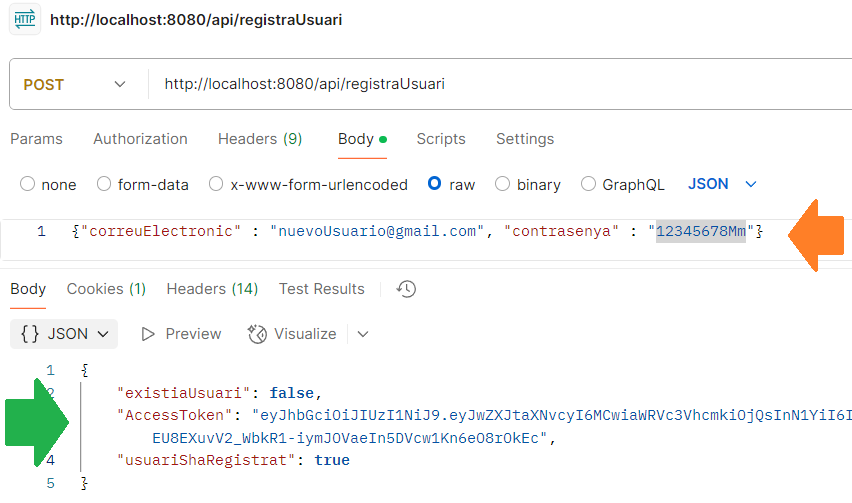
\includegraphics[width=1\textwidth]{img/detallPostmanRegistraUsuari.png}
			\caption{Creación de un nuevo usuario llamando con una solicitud POST al endpoint ``api/registraUsuari'' cuando las validaciones del objeto RegistreDTO del back-end lo permiten. En naranja se muestra el body de la petición (lo que el cliente envía al servidor) y en verde el body de la respuesta (lo que el servidor devuelve al cliente).}
			
			\label{fig:detallPostmanRegistraUsuari} 
		\end{figure}
		\FloatBarrier
		
		
		Tenemos otro endpoint que también expide tokens de acceso, mucho más habitualmente que el anterior: es el endpoint que se consume cuando iniciamos sesión, en \texttt{pas2C\_login.html}: el endpoint ubicado en la URI\footnote{Uniform Resource Identifier} \textit{/api/login}. Si intentamos iniciar sesión con un usuario ya existente en la tabla de usuarios obtendremos algo como esto:
		
		\setlength{\abovecaptionskip}{0pt}
		\FloatBarrier
		\begin{figure}[H]
			\centering
			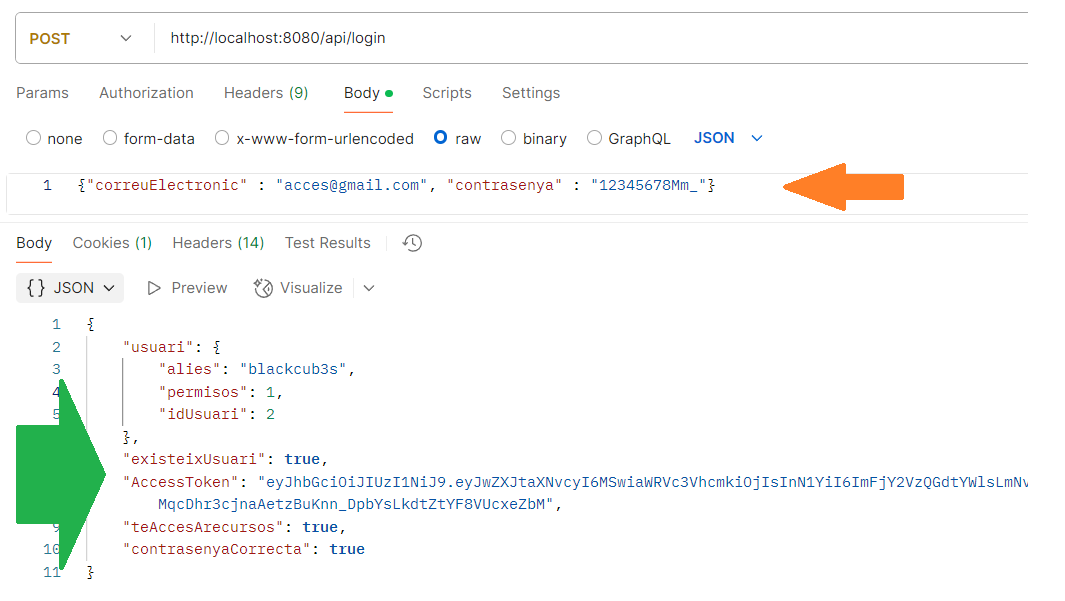
\includegraphics[width=1\textwidth]{img/detallPostmanLogin.png}
			\caption{Iniciando sesión con un usuario ya existente mediante ``api/login'' mandando los datos de ``correuElectronic'' y ``contrasenya'' que leerá y validará el LoginDTO del back-end. En naranja es el body de la petición y en verde el body de la respuesta.}
			
			\label{fig:detallPostmanLogin} 
		\end{figure}
		\FloatBarrier
		
		Por ejemplo podéis ver el endpoint -función de controlador- en GitHub pinchando en el link: \href{https://github.com/blackcub3s/mercApp/blob/78c9f573613d94a9d9de6ee046aa5d6f02f0f425/APP%20WEB/__springboot__produccio__/app/src/main/java/miApp/app/Usuaris/controlador/UsuariControlador.java#L119-L123}{\textit{api/registra-usuari}}. Asimismo podéis hacer lo mismo para el endpoint \href{https://github.com/blackcub3s/mercApp/blob/78c9f573613d94a9d9de6ee046aa5d6f02f0f425/APP%20WEB/__springboot__produccio__/app/src/main/java/miApp/app/Usuaris/controlador/UsuariControlador.java#L103-L107}{\textit{api/login}}. Todo ello son detalles de líneas de código pertenecientes a la clase Spring Boot \href{https://github.com/blackcub3s/mercApp/blob/main/APP%20WEB/__springboot__produccio__/app/src/main/java/miApp/app/Usuaris/controlador/UsuariControlador.java}{ControladorUsuaris.java}
	
		
		\textit{NOTA: La parte de recepción del token en el front-end y de su manejo podéis encontrarla en el apartado \ref{sec:recibirAccesTokenENFRONTEND}}

		
		
		
		
		
		
	
		
		\subsubsection{Recibir en el back-end el JWT enviado desde el front-end y con él securizar un endpoint de la API mediante interpretación de claims y verificación de firma.}
		\label{sec:classesSecuritzacioClaimsIfirma}
		
		Después de crear las tres clases en Java de las que hemos hablado en el apartado \ref{sec:implementacionJWTjava} anterior y haber mandado el token de acceso al front mediante el body de las \textit{responses} a los endpoints \textit{api/registraUsuari} o \textit{api/login}, podemos empezar a 
		implementar la protección de endpoints con JWT. 
		
		Asumamos que nos llega al back-end un token de acceso en una solicitud HTTP de un usuario que ya ha recibido su token y quiere ahora borrar los datos de usuario de otro usuario, es decir, de otro con un idUusario distinto (a través de la heather ``Authorization''). El token sería válido, y este usuario fraudulento tendría el id de permisos igual que el otro usuario propietario de los datos; pero deberíamos, por razones obvias, proteger su acceso.
	
		
		En JavaScript puro, desde el cliente, esta solicitud HTTP de método DELETE la podríamos conseguir de la función \textit{fetch()}, poniéndole uno de los pares clave : valor con el inicio ``Bearer'' (por convenio) tal que así\footnote{Con postman pasamos el token desde la pestaña Authorization y en Auth Type le seleccionamos, en el desplegable, Bearer Token.}:
		
				
\begin{lstlisting}[language=Java, basicstyle=\ttfamily\footnotesize, keywordstyle=\color{magenta}]

fetch("'http://localhost:8080/api/usuaris/{id}'", {
	method: "DELETE",
	headers: {
		"Content-Type": "application/json",
		"Authorization": "Bearer "+tokenJWT;
	},
	...
}
\end{lstlisting}
		
		 Queremos conseguir que ese endpoint permita en cada solicitud \textbf{Autenticarlo}, es decir, determinar que dice ser quien es mediante el hecho de encontrar en el token verificado su \textcolor{red}{idUsuari} correspondiente (y acceder a la información de sus tickets); y a su vez \textbf{Autorizarlo}, es decir, dar acceso a ese usuario a los recursos a los que se le permita acceso mediante la variable \textcolor{orange}{permisos} correspondiente.
		
		 Estos dos pasos irán en función del valor de la variable que haya emanado de la base de datos al conceder el token mediante \textcolor{red}{idUsuari} para el caso de la \textbf{Autenticación} -ver \href{https://github.com/blackcub3s/mercApp/blob/b01cec515bb9af27a1faa24258abb4313ef275cd/APP%20WEB/__springboot__produccio__/app/src/main/java/miApp/app/Usuaris/model/Usuari.java#L30}{linea github}-, y de la variable \textcolor{orange}{permisos} del model de la @Entity class Usuari - ver \href{https://github.com/blackcub3s/mercApp/blob/b01cec515bb9af27a1faa24258abb4313ef275cd/APP%20WEB/__springboot__produccio__/app/src/main/java/miApp/app/Usuaris/model/Usuari.java#L42}{linea github}- para el caso de la \textbf{autorización}). Para ello hay \textbf{tres} pasos que debemos implementar dentro del back-end de SpringBoot:
		
		
		
		
		\begin{itemize} 
			\setlength{\itemsep}{-1.5em}
			\item \textbf{PASO 1:} Extraer la información del usuario autenticado desde \textit{el payload} del token JWT entrante. Para ello crearemos un \textbf{Filtro de Autenticacion} dentro de \texttt{FiltreAutenticacio.java}\\
			\item \textbf{PASO 2:} Configurar el contexto de seguridad para que Spring Security reconozca los permisos, dentro de  \texttt{ConfiguracioSeguretat.java}. \\ 	
			\item \textbf{PASO 3:} Aplicar restricciones con \textbf{@PreAuthorize} en cada \textit{endpoint} que queramos proteger en el controlador, dentro \texttt{UsuariControlador.java}
		\end{itemize}
		

		\noindent \textbf{PASO 1: Extracción del payload (\textit{FiltreAutenticació.java})}
		\hrule
		\vspace{1em}
		
		Esta parte del código está llena de boilerplate. La clase \textit{FiltreAuntenticacioJwt.java} extiende de OncePerRequestFilter \cite{oncePerRequestFilter}, que como dice el propio nombre de la clase implementa un filtro que se desarrollará una y solo una vez por cada petición al servidor.
		
		Lo que hay que hacer aquí es implementar el método \textit{doFilterInternal()} donde colocamos la lógica específica del filtro. Se puede consultar este archivo en github del proyecto \href{https://github.com/blackcub3s/mercApp/blob/main/APP%20WEB/__springboot__produccio__/app/src/main/java/miApp/app/seguretat/FiltreAutenticacioJwt.java}{FiltreAuntenticacioJwt.java}
		
		Lo primero que hay que tener en cuenta al diseñar esta clase es que tenemos que hacer una inyección de dependencias: debemos incluir la clase que hemos diseñado AccessToken para implementar el token de acceso. Lo haremos simplemente incluyéndola en el constructor como un parámetro.
		
		Lo segundo que hay que considerar es la extracción del payload del token (donde tenemos la información que nos permitirá autorizar y autenticar). Para encontrar el token se hace de la \textbf{cabecera} ``Authorization'' de la solicitud HTTP entrante del front-end. La clave es ``Authorization'' y el valor asociado es, por convenio, un String ``Bearer '' concatenado al token de interés; algo así:
		

		
		\FloatBarrier
		\begin{table}[h]
				\centering
 				\textit{``Authorization'' : ``Bearer OJALWQ03P1WNOEGBO...''}
		\end{table}
		\FloatBarrier
		

		 
		  La programación necesaria para conseguir lo mencionado en el párrafo anterior queda recogida en este rango de lineas de GitHub (\href{https://github.com/blackcub3s/mercApp/blob/89efcf854d8bbab2addde3f7e817eb97f7737b95/APP%20WEB/__springboot__produccio__/app/src/main/java/miApp/app/seguretat/FiltreAutenticacioJwt.java#L33-L43}{ver rango}). 
		  
		  Luego una vez tenemos el token dentro de Spring Boot tratamos de sacar las Claims del Payload, es decir, la carga útil del token (\href{https://github.com/blackcub3s/mercApp/blob/89efcf854d8bbab2addde3f7e817eb97f7737b95/APP%20WEB/__springboot__produccio__/app/src/main/java/miApp/app/seguretat/FiltreAutenticacioJwt.java#L50-L54}{ver rango}). Y con ello ya podemos asignar tres roles a partir de la variable permisos del payload: 0, 1 o 2. 
		  
		  0 en la variable permisos de la tabla usuaris de mysql se asigna cuando un usuario ya se ha registrado dando correo y contraseña, pero no ha dado acceso a tickets digitales todavía; 1 en la variable permisos se da cuando el usuario en cuestión ya tiene acceso a la consulta del dashboard de la aplicación (ya se ha registrado y, \textit{además}, concedido acceso a tickets digitales); y 2 se da cuando el usuario en cuestión es superusuario y tiene acceso a consultar todos los recursos de la aplicación, tickets de los demás usuarios, etc. (\href{https://github.com/blackcub3s/mercApp/blob/89efcf854d8bbab2addde3f7e817eb97f7737b95/APP%20WEB/__springboot__produccio__/app/src/main/java/miApp/app/seguretat/FiltreAutenticacioJwt.java#L56-L66}{ver rango}). En definitiva, lo que estamos mencionando (por si el lector se imprimió la memoria y no tiene acceso directo al link de GitHub) las líneas relevantes del código que permiten esa asignación son estas:
		  
		  
		  
		  \begin{lstlisting}[language=Java, basicstyle=\ttfamily\footnotesize, keywordstyle=\color{magenta}]
		  
	Claims claims = accessToken.getClaims(token);
	
	
	Integer permisos = (Integer) claims.get("permisos"); 
	Integer idUsuari = (Integer) claims.get("idUsuari"); 
	
	// Creo autoritat basada en permisos
	String role;
	if (permisos == 2) {
	  	role = "ROLE_ADMIN";
	} else if (permisos == 1) {
	  	role = "ROLE_USER";
	} else {
	  	role = null;
	}
		  
		  \end{lstlisting}
		  
		  Importante es mencionar que en el fragmento de código anterior, al llamar al método $getClaims(token)$  se lanzará una excepción de tipo \textit{ExpiredJwtException} en caso que el token haya expirado, que recogeremos en el primer bloque Catch; y si el token está manipulado y no es válido, entonces se lanzará otra excepción que se recogerá en el segundo bloque Catch. Todo ello se informará como una response al cliente (\href{https://github.com/blackcub3s/mercApp/blob/89efcf854d8bbab2addde3f7e817eb97f7737b95/APP%20WEB/__springboot__produccio__/app/src/main/java/miApp/app/seguretat/FiltreAutenticacioJwt.java#L96-L115}{ver rango de líneas de código}).
		  
		  
		  Y finalmente hay que crear un objeto de tipo \textit{UsernamePasswordAuthenticationToken} ya definido dentro de SpringBoot. Su constructor permitirá tres parámetros: 
		 
		 	\begin{itemize}
		 	\setlength{\itemsep}{-.5em}

			  \item \textbf{el principal}, el primero, al que le pasaremos el \textcolor{red}{idUsuari}
			 \item  \textbf{credentials}, el segundo, que lo dejamos a null porque en JWT no se debe manejar credenciales ya que están contenidas dentro del token. 
			  \item \textbf{una collection con el role}, el tercero, que contendrá los roles que definimos antes. 
		  \end{itemize}
		  Este constructor nos permitirá restringir permisos para las APIs según el \textcolor{red}{idUsuari} al que esté vinculado su login (autenticación) y también según el valor de \textcolor{orange}{permisos} que tenga (autorización)\footnote{Cuidado! Lo cierto es que deben considerarse ambos parámetros a la vez en el controlador, como veremos en el paso 3. No es suficiente añadir roles a un determinado id. Solamente con los roles, Spring Boot no nos dejará, por ejemplo, que en una API que toma el idUsuari como parámetro en la URL (como la de este ejemplo) se pueda restringir a ese usuario específico para que no consulte los recursos de los demás usuarios con idUsuari distintos.}.
		  

		  
		  
 \begin{lstlisting}[language=Java, basicstyle=\ttfamily\footnotesize, keywordstyle=\color{magenta}]
	  	
UsernamePasswordAuthenticationToken authentication = 
new UsernamePasswordAuthenticationToken(
	idUsuari,
	null,
	Collections.singletonList(new SimpleGrantedAuthority(role))
);



 \end{lstlisting}
Este objeto \textit{authentication} que acabamos de crear entonces tenemos que guardarlo DENTRO del SecurityContextHolder:

		 
 \begin{lstlisting}[language=Java, basicstyle=\ttfamily\footnotesize, keywordstyle=\color{magenta}]

 SecurityContextHolder.getContext().setAuthentication(authentication)
	
\end{lstlisting}
	
	
	


		\noindent \textbf{PASO 2: Configuración contexto de seguridad (\textit{ConfiguracioSeguretat.java})}
		\hrule
		\vspace{1em}
		
		Sin esta clase, al añadir la dependencia de seguridad ``spring-boot-starter-security'' en \texttt{pom.xml} cualquier llamada a cualquier API va a devolver un código de error 401. Esto pasa porque al añadir la dependencia de seguridad mencionada nos encontramos con que se precisan ciertas configuraciones. La tres cosas que hay que hacer en la clase \textit{ConfiguracioSeguretat.java} para llevar a término las mencionadas configuraciones son:
		
		
		\begin{itemize}
		\setlength{\itemsep}{-.3em}
		 
		 
		\item \textbf{1. Inyectar jwtAuthenticationFilter}, una instancia de \textit{FiltreAutenticacioJwt.java}, a través del constructor para que actúe como dependencia.
		 
		\item \textbf{2. Especificar que jwtAuthenticationFilter va ANTES del filtro} estándar de Spring para autenticación por usuario/contraseña (\href{https://github.com/blackcub3s/mercApp/blob/db26ff53664be55223c793cf9b52ade87688be45/APP%20WEB/__springboot__produccio__/app/src/main/java/miApp/app/seguretat/ConfiguracioSeguretat.java#L41}{ver línea de código})\footnote{JWT no funciona directamente con Spring Security: su implementación con Spring Security no es directa porque hay que añadir otra dependencia en \textit{pom.xml}, la dependencia``io.jsonwebtoken''. De ahí que debamos decirle a Spring Boot que la utilice no de la forma estandar que tiene spring security.}. 
		
		\item 3. \textbf{Definir endpoints a restringir con \textit{requestMatchers}}: por ejemplo, hay un endpoint que permite cambiar la contraseña de un usuario (una solicitud PATCH). Ese endpoint queda marcado  \href{https://github.com/blackcub3s/mercApp/blob/db26ff53664be55223c793cf9b52ade87688be45/APP%20WEB/__springboot__produccio__/app/src/main/java/miApp/app/seguretat/ConfiguracioSeguretat.java#L34}{en esta línea de ConfiguracioSeguretat.java} y nos define que solo usuario administrador ($permisos = 2$) y usuario de rol ``USER'' ($permisos = 1$) pueden hacer llamadas a él y conseguir cambiar su contraseña:
		
\begin{lstlisting}[language=java, basicstyle=\ttfamily\footnotesize, keywordstyle=\color{magenta}]
.requestMatchers("/api/*/contrasenya").hasAnyRole("USER", "ADMIN")
\end{lstlisting}


		\end{itemize}

			NOTA: La clase ConfiguracioSeguretat.java, en el momento de escribir estas líneas, podéis verla también en el anexo \ref{sec:anexoConfiguracioSeguretat}. Se recomienda ver el \href{https://github.com/blackcub3s/mercApp/blob/main/APP%20WEB/__springboot__produccio__/app/src/main/java/miApp/app/seguretat/ConfiguracioSeguretat.java}{link} actualizado de GitHub de este archivo.
		
		
		\noindent \textbf{PASO 3: Restricciones en el controlador}
		\hrule
		\vspace{1em}
		
		En el endpoint que acabamos de mencionar, todo el trabajo de autenticación y autorización no está hecho todavía. Ahora mismo cualquier usuario con roles ``USER'' (permisos = 1) puede cambiar la contraseña de cualquier usuario. Si este usuario (al que llamaremos X) desea cambiar la contraseña del usuario con idUsuari = 31, por ejemplo, solo deberá mandar una solicitud PATCH dirigida a \textit{``/api/31/contrasenya''} incluyendo el token de acceso de X (sí, aunque su idUsuari sea distinto) con Postman.
		
		¿Esto sería inadmisible, verdad? ¡Si uno fuese el usuario de idUsuari 31 no le haría mucha gracia que otro usuario pudiera cambiar su contraseña! ¡No parece un buen diseño de seguridad!
		
		Para evitarlo no nos queda otra que afinar a nivel de controlador con una anotación denominada @PreAuthorize donde le permitimos a ese controlador en específico afinar quien puede acceder a él. Con esta anotación, pasándole los parámetros adecuados, conseguiremos restringir, si no se es ADMIN, que un solo usuario con un solo idUsuari sea el que pueda cambiar la contraseña (concretamente, este usuari será el del \textit{principal}\footnote{El principal era el idUsuari que pasamos al crear el objeto \textit{UsernamePasswordAuthentitacionToken} dentro del paso1 en \texttt{FiltreAutenticacio.java}.}, el id propio).  El uso de la anotación @PreAuthorize solamente se habilita por parte del framework si en la clase anterior del paso dos añadimos la anotación @EnableMethodSecurity encima del encabezado de la clase \textit{ConfiguracioSeguretat.java} (\href{https://github.com/blackcub3s/mercApp/blob/db26ff53664be55223c793cf9b52ade87688be45/APP%20WEB/__springboot__produccio__/app/src/main/java/miApp/app/seguretat/ConfiguracioSeguretat.java#L16}{link a línea}). Una vez añadida la anotación @EnableMethodSecurity ya podemos ir a \href{		https://github.com/blackcub3s/mercApp/blob/db26ff53664be55223c793cf9b52ade87688be45/APP%20WEB/__springboot__produccio__/app/src/main/java/miApp/app/Usuaris/controlador/UsuariControlador.java#L263}{UsuariControlador.java} y añadir la anotación @PreAuthorize encima de la función correspondiente del endpoint en cuestión \href{https://github.com/blackcub3s/mercApp/blob/db26ff53664be55223c793cf9b52ade87688be45/APP%20WEB/__springboot__produccio__/app/src/main/java/miApp/app/Usuaris/controlador/UsuariControlador.java#L263}{(ver en contexto)}, tal que así:
		
\begin{lstlisting}[language=java, basicstyle=\ttfamily\footnotesize, keywordstyle=\color{magenta}]
	@PreAuthorize("hasRole('ADMIN') or #id == principal")
\end{lstlisting}

	NOTA: Podéis ver la función completa del controlador en el anexo \ref{sec:detallSeguretatControlador}
	
	
		
		

		
		
			\subsection{Validación de datos (endpoints back-end)}
			\label{sec:validacioDadesBACK}
			
			\textit{NOTA: Los datos validados en el back-end siguen las mismas expresiones regulares y restricciones que las validaciones hechas en el front-end (ver sección \ref{sec:validacioDadesFRONT}).}
			
			Los endpoints del back-end a los que apuntamos con llamadas fetch desde los campos de formulario de correo electrónico y contraseña desde el HTML deben protegerse también en el back-end, no solamente en el front.
			
			El motivo de ello es porque no podemos permitir que entren unos datos no validados (nulos, con caracteres peligrosos, etc) a través de \textbf{llamadas directas a la API}. Hay que tener mucho cuidado con esto! 
			
			La parte donde definimos la validación de datos de los endpoints de entrada de los datos de usuario está en utils\footnote{podéis ver la imagen completa de la estructura del proyecto SpringBoot si queréis, de nuevo, en \ref{fig:estrucutraAplicacioJAVARESOURCES}} pero se produce parte de validación a través de \textit{Usuaris} $\rightarrow$ \textit{dto}. Una primera aproximación o esquema a entender como se interelacionan estos dos tipos de clases está en la figura \ref{fig:validacioBackArxius}.
			
			
			
			\FloatBarrier
			\setlength{\belowcaptionskip}{3pt}
			\begin{figure}[H]
				\centering
				\caption{\textbf{Izquierda}: Archivos de clases de anotación (@), la clase donde se definen mensajes de error que aprovecharán las clases de anotación $|$  \textbf{Derecha}: los DTOs o \textit{Data Transfer Objects} que es donde se aplican las validaciones definidas en las clases de anotación.}
				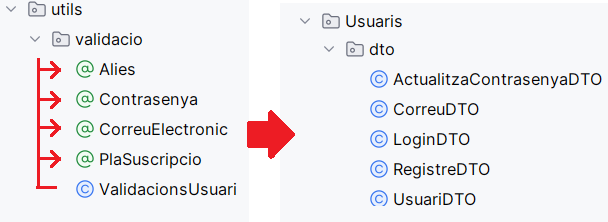
\includegraphics[width=.8\linewidth]{img/validacioBackArxius.png}
				\label{fig:validacioBackArxius}
			\end{figure}
			\FloatBarrier
			
			
			Vamos a hablar en términos concretos. Pongamos por caso que queremos validar los datos de entrada que llegan a través del endpoint que recibe la llamada POST del front-end para el inicio de sesión, es decir, el endpoint ``\href{https://github.com/blackcub3s/mercApp/blob/4ddc34194763af7a246ffabb14146ad9b4b2c5db/APP%20WEB/__springboot__produccio__/app/src/main/java/miApp/app/Usuaris/controlador/UsuariControlador.java#L103}{api/login}'' del archivo \href{https://github.com/blackcub3s/mercApp/blob/main/APP%20WEB/__springboot__produccio__/app/src/main/java/miApp/app/Usuaris/controlador/UsuariControlador.java}{ControladorUsuari.java} de Spring Boot. 
			
			Debemos entender que en este caso, cuando se haga una llamada exitosa a ese controlador, tendremos un \textit{body} del estilo siguiente:
			
				
			\begin{lstlisting}[language=xml, basicstyle=\ttfamily\footnotesize, keywordstyle=\color{magenta}]
{"correuElectronic" : "acces@gmail.com", "contrasenya" : "12345678Mm\_" }
			\end{lstlisting}
			
	
			

			
			Según los términos esperados las clases utilizadas y activadas para validar estos datos de entrada serán las de la figura \ref{fig:validacioBackArxiusDetallLoginVA}:
			
			
			
			\FloatBarrier
			\setlength{\belowcaptionskip}{3pt}
			\begin{figure}[H]
				\centering
				\caption{Activación de clases de validación para responder a una solicitud POST de inicio de sesión hecha hacia el endpoint \textit{/api/login} del controlador UsuariControlador.java}
				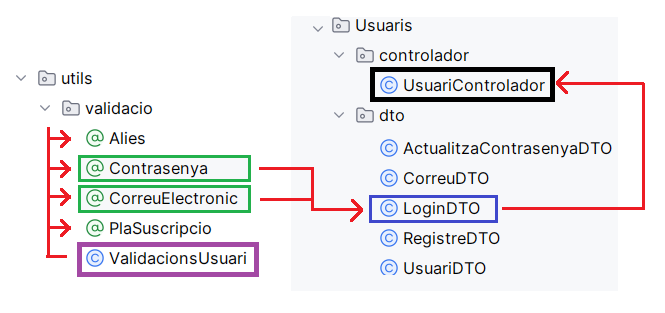
\includegraphics[width=1\linewidth]{img/validacioBackArxiusDetallLoginVA}
				\label{fig:validacioBackArxiusDetallLoginVA}
			\end{figure}
			\FloatBarrier
			
			
			 Asimismo, en la figura  \ref{fig:validacioBackArxiusDetallLoginVB} podréis ver exactamente qué es lo que está pasando para la llamada a este endpoint. Podréis ver en esencia como existe una clase LoginDTO\footnote{Los data transfer objects o DTOs son simplemente clases Java que mediante sus atributos definen los nombres exactos que tienen que tener las claves entrantes del body de las solicitudes POST y, además, aplican restricciones a los valores que éstas llevan asociadas según unas anotaciones definidas encima, que asimismo llaman a otras anotaciones de las clases de anotación, si y solo si, añadimos la anotación \textbf{@Valid} antes del parámetro dto del UsuariControlador.} que permite hacer la validación de datos cuando un usuario inicia sesión, a través de anotaciones personalizadas (@CorreuElectronic y @contrasenya) que a su vez llaman a otras anotaciones propias del framework springboot (@pattern, para aplicar expresiones regulares; @NotBlank para evitar que el campo esté vacío, etc):
			
			
			

			
			
			\FloatBarrier
			\setlength{\belowcaptionskip}{3pt}
			\begin{figure}[H]
				\centering
				\caption{Veremos que en \textit{UsuariControlador.java} (imagen de la derecha) el tipo de datos que espera el endpoint \textit{api/login} se guarda en el parámetro de entrada \textit{dto}. Esto pasa gracias a la anotación \textbf{@RequestBody} que mapea la entrada en formato JSON con el parámetro de entrada que esté a su derecha: en este caso \textit{dto}. dto tiene que tener un formato compatible con los datos JSON entrantes por el body de la solicitud POST, obviamente. El dto está tipado con \textit{LoginDTO}, que es una clase que hemos definido nosotros y permite recoger los datos entrantes hacendo un match entre los nombres de las claves del JSON y los nombres de los atributos de la clase. Esta clase también permite definir las validaciones mediante anotaciones personalizadas, que están justamente encima de cada atributo y permiten validar los datos para ese atributo. Estas anotaciones en LoginDTO se activan si y solo si \textit{UsuariControlador.java} tiene definida la anotación \textbf{@Valid} al lado del parámetro dto. Las dos anotaciones personalizadas de LoginDTO son \textbf{@Contrasenya} y \textbf{@CorreuElectronic} que llaman asimismo a otras clases de anotación ya definidas del lenguaje: \textit{@pattern}, para aplicar expresiones regulares o \textit{@NotBlank} para evitar que el campo esté vacío}.
				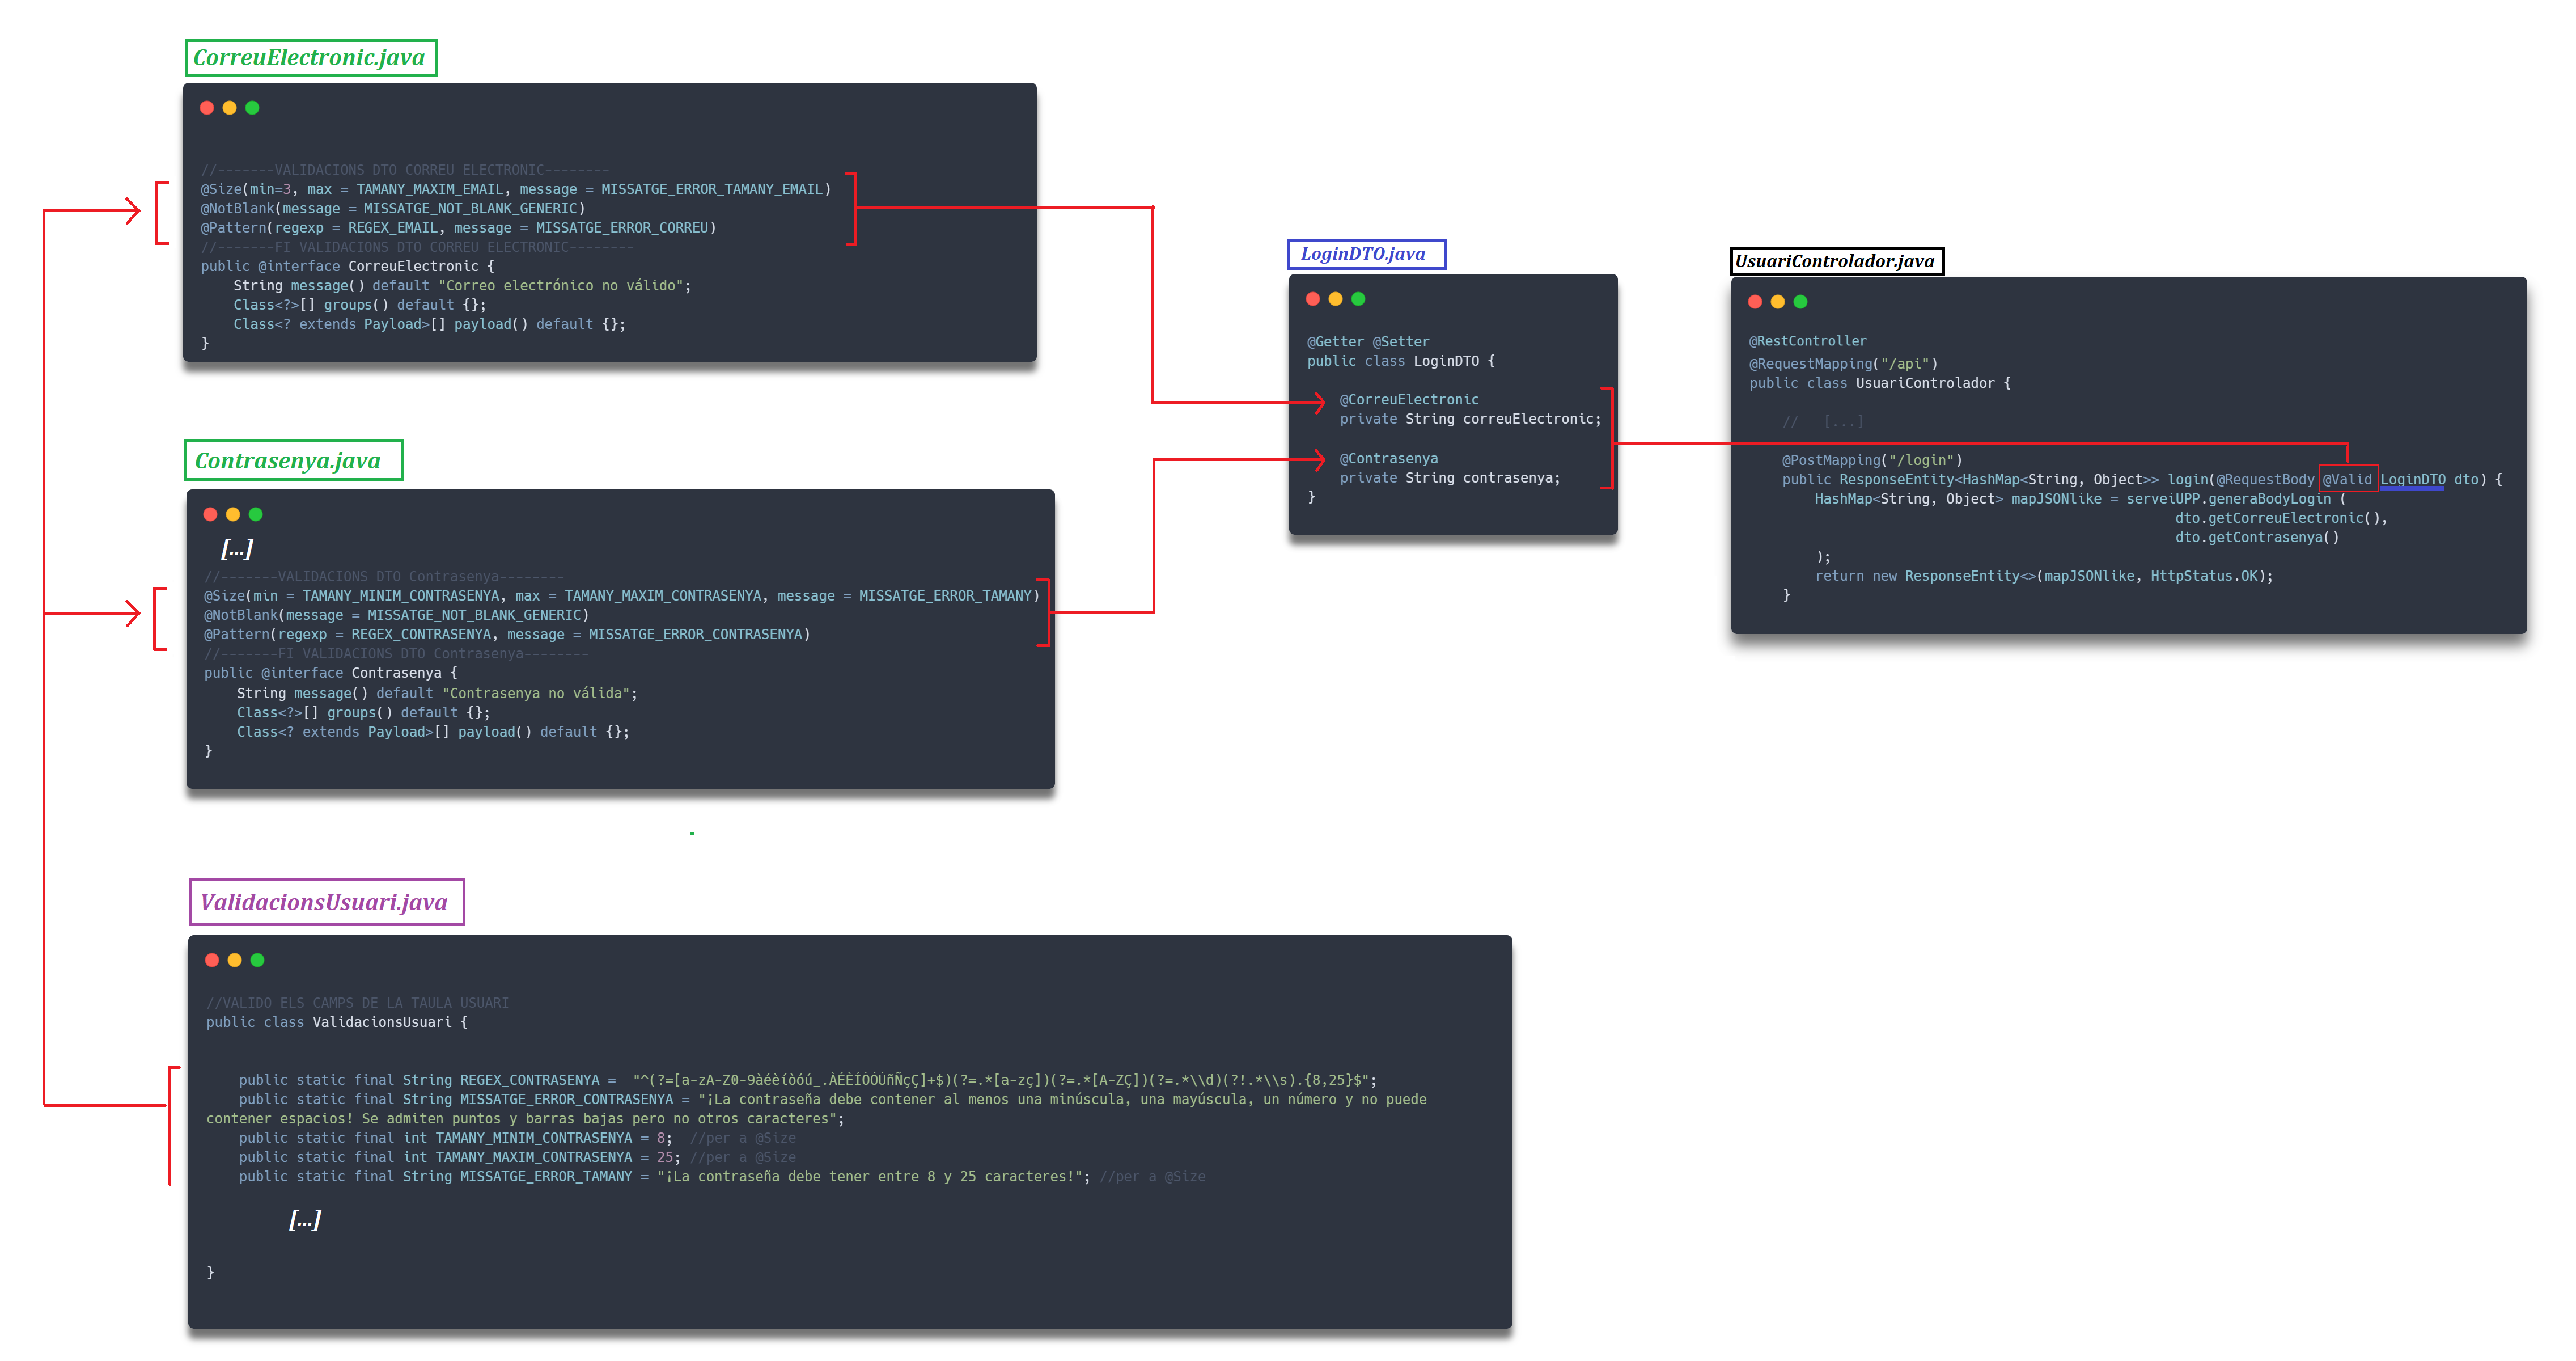
\includegraphics[width=1\linewidth]{img/validacioBackArxiusDetallLoginVB}
				\label{fig:validacioBackArxiusDetallLoginVB}
			\end{figure}
			\FloatBarrier
			
		
			Podría parecer complejo hacer lo que hemos hecho en la figura \ref{fig:validacioBackArxiusDetallLoginVB}, pero una vez guardarmos campos en la base de datos a través de múltiples endpoints que requieren modificaciones parciales de esos campos hacerlo así tiene utilidad y es una buena práctica en Java.
			
			Todos los endpoints de la clase UsuariControlador.java están protegidos con validaciones para evitar que entren caracteres problemáticos, como podéis ver en las expresiones regulares definidas en ValidacionsUsuari.java.

			\subsection{Hasheado de contraseñas}
			\label{sec:implementacioHashContra}
			
			Las contraseñas de los usuarios no se han guardado en texto plano. Por seguridad, se han guardado en forma de hash, es decir, con encriptación unidireccional. A tal efecto se ha utilizado la librería bcrypt de Spring security\cite{bcryptPasswordEncoder} y se ha hecho una clase \href{https://github.com/blackcub3s/mercApp/blob/main/APP%20WEB/__springboot__produccio__/app/src/main/java/miApp/app/utils/EncriptaContrasenyes.java}{EncriptaContrasenyes.java} que ha permitido envolver con nombres más pedagógicos las funciones de bcrypt que han sido usadas  (ver figura \ref{fig:hashejatContrasenyes}).
			
			\FloatBarrier
			\begin{figure}[H]
				\centering
				\caption{Clase \texttt{EncriptaContrasenyes.java}, utilizada para encriptar contraseñas y comparar hash encriptados.}
				\label{fig:hashejatContrasenyes}
				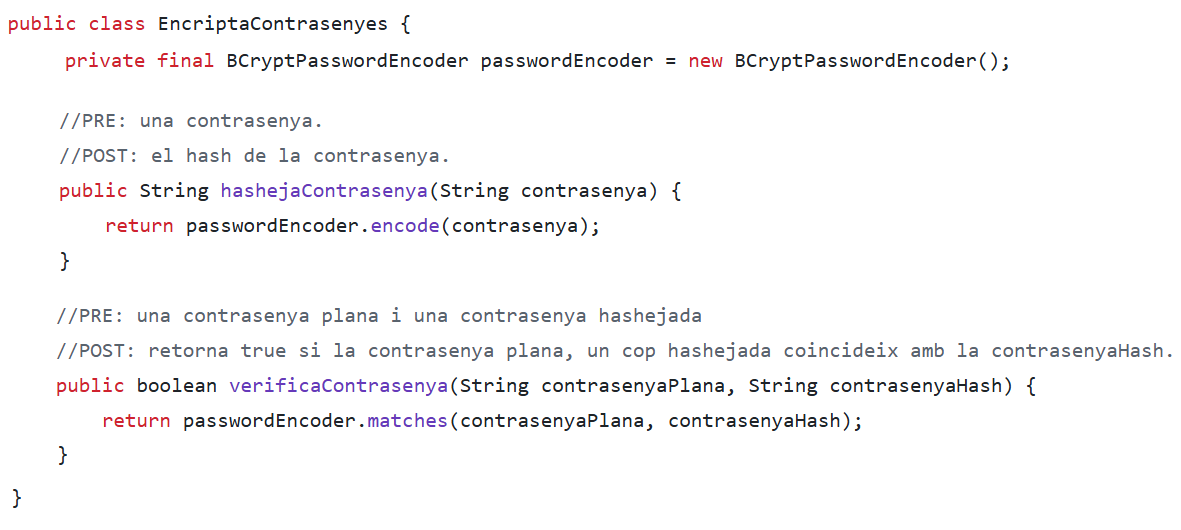
\includegraphics[width=1\linewidth]{img/hashejatContrasenyes.png}
			\end{figure}
			\FloatBarrier
			
			Específicamente, cada vez que un usuario inicie sesión o se registre, se utilizarán una u otra función de la clase \href{https://github.com/blackcub3s/mercApp/blob/main/APP%20WEB/__springboot__produccio__/app/src/main/java/miApp/app/utils/EncriptaContrasenyes.java}{EncriptaContrasenyes.java}. Al instanciar un objeto de la misma, se instanciará también un objeto BCryptPasswordEncoder y se usarán las funciones de librería \textit{encode()}\footnote{Para obtener el hash de una contraseña creada.} y \textit{matches()}\footnote{Para verificar si una contraseña plana es coincidente con el hash que se guardó en base de datos en el momento del registro.}, respectivamente (convenientemente guardadas con un nombre más agradable como vemos en la figura \ref{fig:hashejatContrasenyes}).
			
			Esto se hará en la clase de servicio \textit{UsuariServei.java}. Por ejemplo, para el inicio de sesión el uso de \textit{matches()} a través de \textit{ verificaContrasenya()} lo encontraremos en esta línea de código de dicha clase:  \href{https://github.com/blackcub3s/mercApp/blob/e8afa7110971dca00a660bd8ec5f1a565b852fbd/APP%20WEB/__springboot__produccio__/app/src/main/java/miApp/app/Usuaris/servei/UsuariServei.java#L67}{link}.
			

			
			
			¡Es interesante hacer notar que una misma contraseña encriptada varias veces por la función \textit{encode()} (envuelta en \textit{hashejaContrsenya()}) produce hash distintos! Es decir, el hashing no solo imposibilita ver las contraseñas de los usuarios, sino que también impide ver si dos usuarios tienen la misma contraseña. Esto también hace que no podamos comparar con una función simple de comparación de strings el hash guardado de una contraseña en el momento del registro con el hash generado por un logueo. Por eso nos vemos obligados a usar el metodo \textit{matches()}.
			
			
			
			
			

			
	\section{Desarrollo back-end (FastAPI, Python)}
	
	\subsection{Contenerización}
	\label{sec:conteneritzacioPython}
	
	Este microservicio lo contenerizaremos gracias a este \href{https://github.com/blackcub3s/mercApp/tree/main/APP%20WEB/__FastAPI__/Dockerfile}{Dockerfile}. Para hacerlo, usaremos el Dockerfile para crear una imagen desde la imagen python:3-11 alpine\footnote{Las imágenes alpine son ligeras: pesan 100 o 200MB a diferencia de las que provienen de la imagen entera de python, que pesan más de 1GB.} descargada del registry de docker (ver nota sobre instalación de docker\footnote{ Instalar docker en linux no se puede hacer con un solo comando. Si el lector lo quiere instalar y usa linux, le facilito el script que programé hace un tiempo, para poder instalarlo sin preocuparse de nada: \href{https://github.com/blackcub3s/mercApp/blob/main/auxiliars/instalaDocker.sh}{link}. Si el lector usa Windows solamente debe preocuparse de instalar docker desktop y asegurarse que se añade la docker CLI para poder usar comandos desde las terminales disponibles en el sistema.}). 
	
	Para crear la imagen con este Dockerfile, para hacer pruebas y ver como se despliega el contenedor, el lector puede probar de crear una imagen denominada ``back-end-fastapi''. Para hacerlo puede moverse a donde está el Dockerfile y ejecutar el siguiente subcomando de docker (\textit{build}), tal que así:
	
	\begin{lstlisting}[language=bash]
		docker build -t back-end-fastapi .
	\end{lstlisting}
	
		Ahora la imagen ``back-end-fastapi'' ya está creada y con docker images veremos que así es (figura \ref{fig:dockerimages}):
	\FloatBarrier
	\begin{figure}[H]
		\centering
		\caption{comando docker images para ver las imágenes creadas}
		\label{fig:dockerimages}
		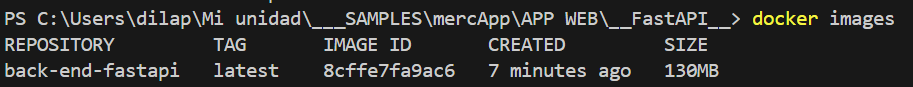
\includegraphics[width=1\linewidth]{img/dockerImages}
	\end{figure}
	\FloatBarrier
	

	
	Acto seguido, una vez ya creada la imagen que contendrá todo el sistema de archivos de la aplicación con Python y sus dependencias (\textit{pip install ...}), debemos usar esta imagen para derivar de ella un contenedor (es decir, crear una instancia de esa imagen). Crearemos el contenedor de nombre \textit{contFastApi} a partir de la imagen anterior y le pediremos que exponga el puerto 8000\footnote{Hace referencia al 8000 que va a la \textbf{derecha} de los dos puntos.} -puerto con el que se comunica FastAPI en el interior del contenedor- y haremos que exponga ese puerto también al exterior del contenedor\footnote{Es el 8000 emplazado a la \textbf{izquierda} de los dos puntos.}. Podemos hacerlo con run o con create. En este caso con create porque no queremos todavía arrancar el contenedor:
	
	\begin{lstlisting}[language=bash]
docker create -p 8000:8000 --name contFastApi back-end-fastapi
	\end{lstlisting}

	
	Una vez creado el contenedor ya podemos arrancarlo. Aqui ya no hay que definir puertos nuevamente porque ya se definieron al crear la imagen. Es también opcional usar las flags -a\footnote{Simplemente veremos lo que imprima la terminal} e -i\footnote{Nos permitiría interaccionar con el programa a través de la terminal si fuese necesario}:
	
	\begin{lstlisting}[language=bash]
		docker start -ai contFastApi
	\end{lstlisting}
	
	
	Ahora el contenedor se podría acceder a través de otro contenedor. Nótese que  \href{https://github.com/blackcub3s/mercApp/blob/cf678ebf99ce636b64c70c8faa239658a601550d/APP%20WEB/__FastAPI__/Dockerfile#L22}{en esta línea} del dockerfile hemos definido el host de la aplicación FastAPI desde dentro del contenedor para que sea la IP 0.0.0.0 . \textbf{No }hemos usado la IP loopback por defecto (localhost, loopback o 127.0.0.1), sino la IP ``wildcard'' o dirección de red (0.0.0.0). Si usáramos la localhost dentro del contenedor la aplicación estaría usando la direccion de dentro de la red del contenedor, pero no saldría fuera de este y sería inútil! La dirección 0.0.0.0 nos permite justamente que podamos acceder a los endpoints de FastAPI desde el localhost del sistema host no solo desde el localhost del propio contenedor. Es decir, nos permite que podamos acceder desde el navegador de nuestro ordenador -desde fuera del contenedor- o desde otros contenedores que estén corriendo en nuestra máquina. Véase en la figura \ref{fig:demofastapiendpointdummy} siguiente lo que puede hacer nuestro contenedor con esta configuración y como se construye, de forma más pormenorizada:
	
	\FloatBarrier
	\begin{figure}[H]
		\centering
		\caption{definición de un endpoint de FastApi que correrá dentro del contenedor docker contFastApi (subcaptura A)), configuración del comando para correr FastAPI dentro de los contenedores que se instancien a partir de la imagen del Dockerfile, con la dirección de red 0.0.0.0 que permite exponer endpoints de contenedores que se creen con la misma fuera de esos contenedores (B) rectángulo rojo). También podemos ver la configuración de que FastAPI correrá en el puerto 8000 \textbf{dentro} del contenedor instanciado (B) rectángulo verde). Finalmente, podemos ver también el comando que crea finalmente contenedor desde la imagen, pidiéndole que que escuche en el puerto 8000 de la red interna del contenedor (C) rectángulo verde) y lo de ahí lo saque al puerto 8000 (C) rectángulo naranja) siendo el resultado de la exposición del endpoint observable en nuestro equipo anfitrión del contenedor en el localhost en ese mismo puerto 8000 (D), rectángulo naranja).}
		\label{fig:demofastapiendpointdummy}
		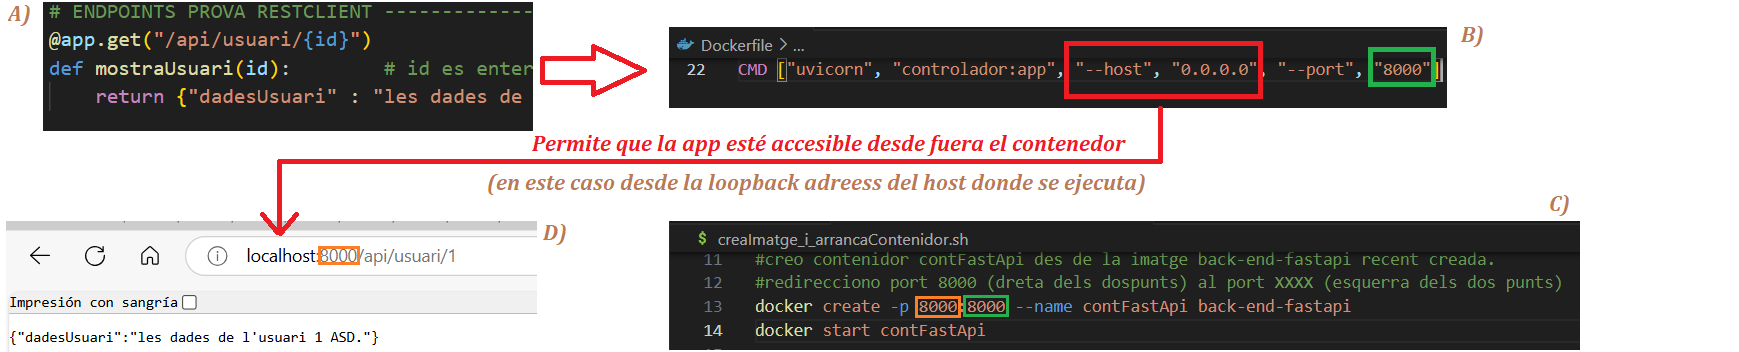
\includegraphics[width=1\linewidth]{img/demoFastApiEndpointDummy}
	\end{figure}
	\FloatBarrier
	
	Para automatizar el proceso de crear imagen con FastAPI y arrancar contenedor desde esta imagen y, finalmente, exponer los endpoints de FastAPI fuera del contenedor, puede usarse el script en bash \href{https://github.com/blackcub3s/mercApp/blob/main/APP%20WEB/__FastAPI__/creaImatge_i_arrancaContenidor.sh}{creaImatge\_i\_arrancaContenidor.sh}, que incluye todos los comandos necesarios (inclusive aquellos para parar y destruir contenedores antiguos).
	
	\subsection{estructura de la aplicación}
	
	\begin{figure}[H]
		\centering
		\caption{La estructura escogida simula un proyecto de Spring Boot: no es la arquitectura que se utiliza por defecto en FastAPI; pero dado que estamos acostumbrados a Java así se ha hecho. Todos los archivos están en una misma carpeta -que es evidentemtente mejorable a nivel de patrón de diseño-.}
		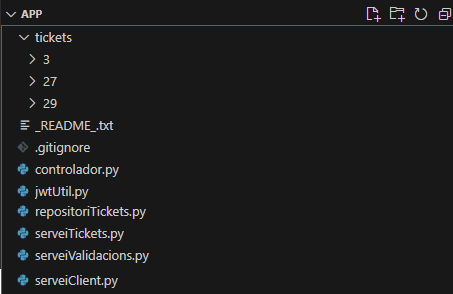
\includegraphics[width=.7\linewidth]{img/estructuraSeguidaFastAPI}

		\label{fig:estructuraseguidafastapi}
	\end{figure}
	
	 En la figura \ref{fig:estructuraseguidafastapi} podemos ver los archivos Python (extensión .py). El \href{https://github.com/blackcub3s/mercApp/blob/main/APP%20WEB/__FastAPI__/app/controlador.py}{controlador.py} incluye los endpoints (la API de los tickets); \href{https://github.com/blackcub3s/mercApp/blob/main/APP%20WEB/__FastAPI__/app/serveiTickets.py}{serveiTickets.py}, \href{https://github.com/blackcub3s/mercApp/blob/main/APP%20WEB/__FastAPI__/app/serveiValidacions.py}{serveiValidacions.py} y \href{https://github.com/blackcub3s/mercApp/blob/main/APP%20WEB/__FastAPI__/app/serveiClient.py}{serveiClient.py} implementan la lógica de negocio usada para parsear tickets en PDF, validar sus tamaños y nombres de archivo, y para hacer llamadas HTTP al otro back-end -Spring Boot-, \textbf{respectivamente}. Finalmente la clase de servicio que extre los tickets (serveiTickets.py) hace uso de  \href{https://github.com/blackcub3s/mercApp/blob/main/APP%20WEB/__FastAPI__/app/repositoriTickets.py}{repositoriTickets.py}, que es donde definiremos las operaciones de persistencia para guardar y leer tickets de mongoDB. \href{https://github.com/blackcub3s/mercApp/blob/main/APP%20WEB/__FastAPI__/app/jwtUtil.py}{jwtUtil.py} se ha utiliado para leer los tokens de acceso. la carpeta tickets incluye subcarpetas de creación automática que los usuarios crean cuando suben los tickets en PDF físicos al servidor (como veremos es un paso que precede a la extracción con parseo a formato estructurado y posterior guardado en MongoDB). Nótese que aquí no usamos un model porque Python no es un lenguaje tan orientado a objetos como java y haberlo incluido hubiese ido en contra de la simplicidad que ya nos brinda el lenguaje.
	 
\textit{NOTA: Para más información de la estructura ``controller'' (controlador), ``service'' (servicio), ``repository'' (repositorio) y ``model'' (modelo) podéis ver el apartado de Spring Boot donde se comenta más en detalle este tipo de arquitectura \ref{sec:classesProjecteSpringboot}.}
	 
	   
	\subsection{Solicitud de subida y parseo de datos}
	\label{sec:solicitudDeExtraccion}
	
	
	\textbf{NOTA:} \textit{las peticiones POST con JavaScript desde el front-end hacia los end points de subida de PDFs y de parseo de PDFs, que mostraremos en las próximas líneas del lado del servidor, ya se mencionaron como se activan mediante el front-end en la PARTE 2 y 3 del apartado \ref{sec:pas4googleAPIclient}, dedicado exclusivamente a JavaScript en el front-end.}
	
	A continuación mostramos los 4 pasos o partes, que deberán ejecutarse \textbf{secuencialmente} y \textbf{con éxito} para que un usuario durante el proceso de registro pueda adjuntar tickets y luego se parseen y guarden en la base de datos. Las partes 1, 2, 3 y 4 que mostraremos a continuación tienen correspondencia con las letras \textit{f}, \textit{g}, \textit{h}, y finalmente, \textit{j} de la figura esquemática anterior \ref{fig:diagramaSistemesAplicacioMercappCAMIREGISTRE}, que suponía el esquema de sistemas de la aplicación en la fase de registro del usuario en el apartado preliminar de diseño:
	
	\begin{itemize}
	\setlength{\itemsep}{-.3em}
		\item \textbf{PARTE 1}: FastAPI recibe la POST \textbf{request} en el endpoint \href{https://github.com/blackcub3s/mercApp/blob/1394c4a58c59d41e1b64f1113007277676fe4cf8/APP%20WEB/__FastAPI__/app/controlador.py#L37}{/api/subir-tickets-pdf} con los tickets adjuntos desde el cliente y con el \textit{token de acceso} con permisos a 0 [\ref{sec:PARTE1_FASTAPI}]\footnote{0 es el caso de uso más frecuente, pero también podría ser 2 si fuese admin. Ese token lo expidió Spring Boot al acceder a pas4, pero ahora lo usa fastAPI para permitir acceso a su API.}.
		\item \textbf{PARTE 2}: FastAPI recibe una solicitud POST en el endpoint \href{https://github.com/blackcub3s/mercApp/blob/8f9e4de79e8f384a9da6e0c43222135d5d8e3bd2/APP%20WEB/__FastAPI__/app/controlador.py#L116}{/api/parsea-y-guarda-pdfs-en-bbdd} que consigue que el servidor parsee con un algoritmo de extracción todos los tickets subidos en \textit{PARTE 1} [\ref{sec:PARTE2_FASTAPI}].
		\item \textbf{PARTE 3}: FastAPI manda a MongoDB los datos de los tickets parseados [\ref{sec:PARTE3_FASTAPI}].
		\item \textbf{PARTE 4}: FastAPI manda el token de acceso (con permisos a 0) hacia Spring Boot, que actualiza permisos en bbdd mySQL (taula usuaris), y manda de vuelta un nuevo token (con permisos a 1) [\ref{sec:PARTE4_FASTAPI}].
	\end{itemize}

	
	NOTA: A modo de recordatorio, hay que decir que después de la PARTE 4, al recibir en el front-end el nuevo token de acceso con permisos a 1, la página \texttt{pas4\_concedirAccesGmail.html} redirigirá automáticamente al dashboard sin que tengamos que hacer nada más (vuélvase a ver lógica de redirecciones en la figura \ref{fig:restringeixVistesPrivadesUSUARINOLOGUEJAT}).
	
		
		

		
		\subsubsection{PARTE 1: FastAPI recibe la POST request en el endpoint /api/subir-tickets-pdf con los tickets adjuntos desde el cliente y con el token de acceso con permisos a 0}
		\label{sec:PARTE1_FASTAPI}
		
		Con la solicitud HTTP mencionada hacia el endpoint \href{https://github.com/blackcub3s/mercApp/blob/1394c4a58c59d41e1b64f1113007277676fe4cf8/APP%20WEB/__FastAPI__/app/controlador.py#L111-L128}{/api/subir-tickets-pdf}\footnote{Recordamos que se produce al clicar al icono del clip en el pas4.} lo que consigue un usuario es adjuntar los PDFs del ordenador del usuario al sistema de archivos del servidor (la validación de datos de este endpoint se especifica en sección \ref{sec:validacioDadesApiSubirtickets}).
		
		\subsubsection{PARTE 2: FastAPI parsea todos los tickets con un algoritmo de extracción}
		\label{sec:PARTE2_FASTAPI}
		
		Para iniciar el parseo de ficheros se empieza con una llamada POST al endpoint \href{https://github.com/blackcub3s/mercApp/blob/f5413ed8cf7ed88c5ed18299564b836d27c52bd4/APP%20WEB/__FastAPI__/app/controlador.py#L132-L152}{/api/parsea-y-guarda-pdfs-en-bbdd}\footnote{Recordamos que esta llamada se hace con el click al engranaje del pas4.}. El algoritmo de extracción se encuentra en el archivo \href{https://github.com/blackcub3s/mercApp/blob/main/APP%20WEB/__FastAPI__/app/serveiTickets.py}{serveiTickets.py} al que llamamos desde el endpoint mencionado y su programación ha sido posible gracias a la existencia de la librería PyPDF2 \cite{PyPDF2}.
		
		El correo electrónico más antiguo y más nuevo contienen tickets que prácticamente no difieren. Por ello el algoritmo de extracción servirá para todos los tickets de Mercadona: como podemos ver en la imagen \ref{fig:primerIultimTiketMeuCorreu}.
		
		
		
		\FloatBarrier
		\setlength{\belowcaptionskip}{3pt}
		\begin{figure}[H]
			\centering
			\caption{A la \textbf{izquierda}: la primera compra en Mercadona que hice en 2023 con ticket digital, en un supermercado en Catalunya; a la \textbf{derecha} la última compra que se hizo: en la Comunitat Valenciana. Nótese que en la extracción hay que tener en cuenta el distinto idioma que se puede dar en distintas comunidades autónomas (Euskadi, Galicia no han sido testeadas). La dirección de correo desde la que se mandan los tickets digitales no ha cambiado en dos años y el formato general del ticket es exactamente igual en términos de parseo: hay que prestar, empero, atención a posibles problemas con UNICODE (círculo marrón) en tickets antiguos.}
			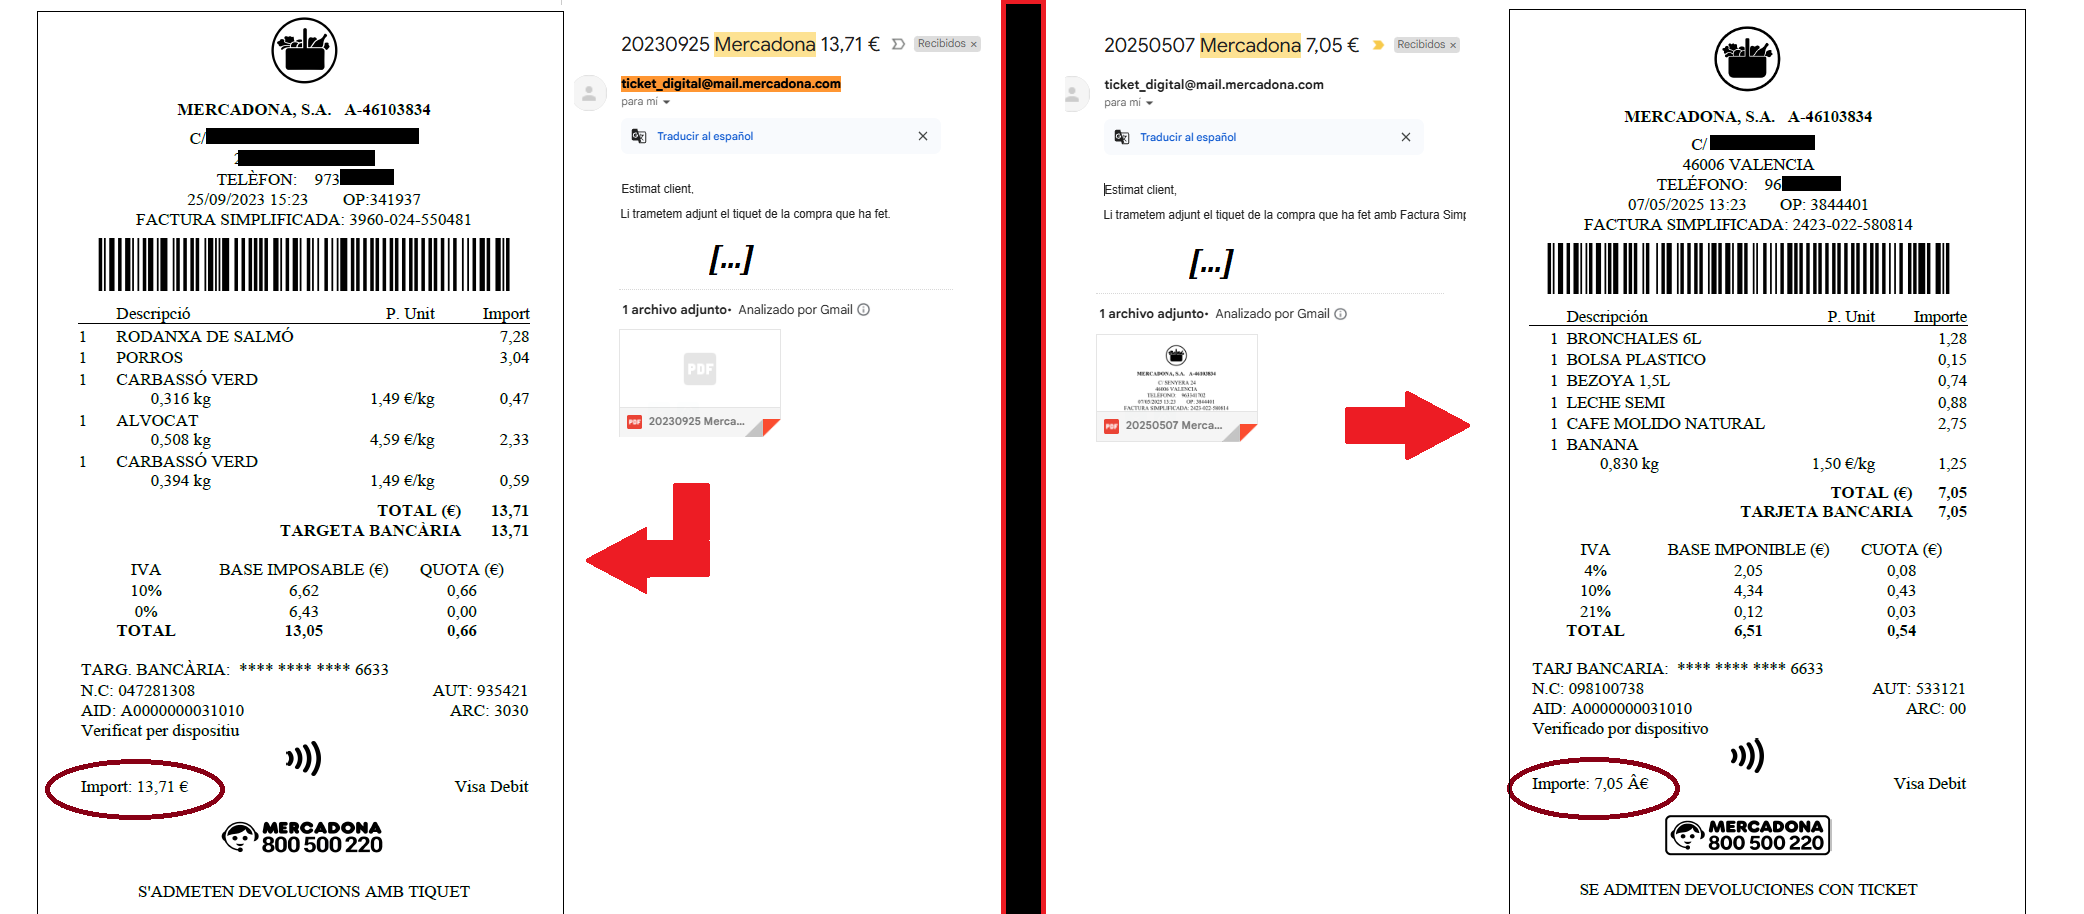
\includegraphics[width=1\linewidth]{img/primerIultimTiketMeuCorreu}
			\label{fig:primerIultimTiketMeuCorreu}
		\end{figure}
		\FloatBarrier
		
		Por ejemplo, el parseo del ticket de la derecha de la figura anterior \ref{fig:primerIultimTiketMeuCorreu} se convertirá en formato JSON después del parseo. Para conseguirlo, se introduce a un diccionario\footnote{Un diccionario en Python es como un HashMap de Java o un Javascript Object: con una estructura de pares clave:valor.} de Python que luego se podrá guardar directamente en una colección de MongoDB con un formato estructurado compacto (figura \ref{fig:ticketJsonEstructuratMostra}) o ampliado si queremos más legibilidad (figura \ref{fig:ticketJsonEstructuratMostraAMBCLAUS})\footnote{MongoDB no guarda JSON exactamente. Lo que hace es guardar objetos BSON (binary JSON) que son una representación binaria del JSON, pero que en esencia está optimizada para rendimiento en operaciones de consulta y escritura y, también, para que ocupe menos espacio que un JSON no binario (texto plano).}.
		
		Hagamos lo que hagamos vamos a recorrer todas las lineas con la función \textit{fesScrapTicketMercadona()} del fichero \href{https://github.com/blackcub3s/mercApp/blob/main/APP%20WEB/__FastAPI__/app/serveiTickets.py}{serveiTickets.py} y extraeremos los datos más importantes del ticket. Para hacerlo debemos tener en cuenta que el layout del ticket es distinto si tratamos de parsear un producto a granel o bien si es un producto que se vende a un precio unitario: los productos a granel, a diferencia de los que no lo son, ocupan dos líneas en el ticket porque añaden una línea más donde se añaden el precio por kg y el precio total. Además, otra diferencia, es que en la misma línea del nombre del producto no sale el precio o importe (porque sale en la segunda).
		
		Esto es una fuente de variabilidad que encontraremos en cada ticket y se tendrá que tener en cuenta al tratar el string del ticket. Dentro de la función \textit{fesScrapTicketMercadona()} vamos a tener en cuenta estos aspectos y los vamos a comentar en el código.
		
		Una parte amable del ticket es que ya incluye, en principio, una clave candidata a ser clave primaria. Si concatenamos la factura simplificada con OP (número de operación) deberíamos tener algo que nunca -salvo rarísimas excepciones- se repite.
		
		
		
		
		\FloatBarrier
		\setlength{\belowcaptionskip}{3pt}
		\begin{figure}[H]
			\centering
			\caption{Formato en el que parsearemos cada ticket digital de Mercadona para poder guardarlo en MongoDB y habilitar consultas eficientes. $|$Dentro de cada producto hay una lista que indica respectivamente si el producto es granel (0 si no lo es, 1 si sí lo es). Entonces, el segundo elemento de la lista indica el precio unitario o el precio por kg (en función de si es granel o no lo es, respectivamente); el tercer elemento, indica el número de unidades compradas o el número de kg comprados (en función del primer parámetro); el cuarto elemento es la categoria.}
			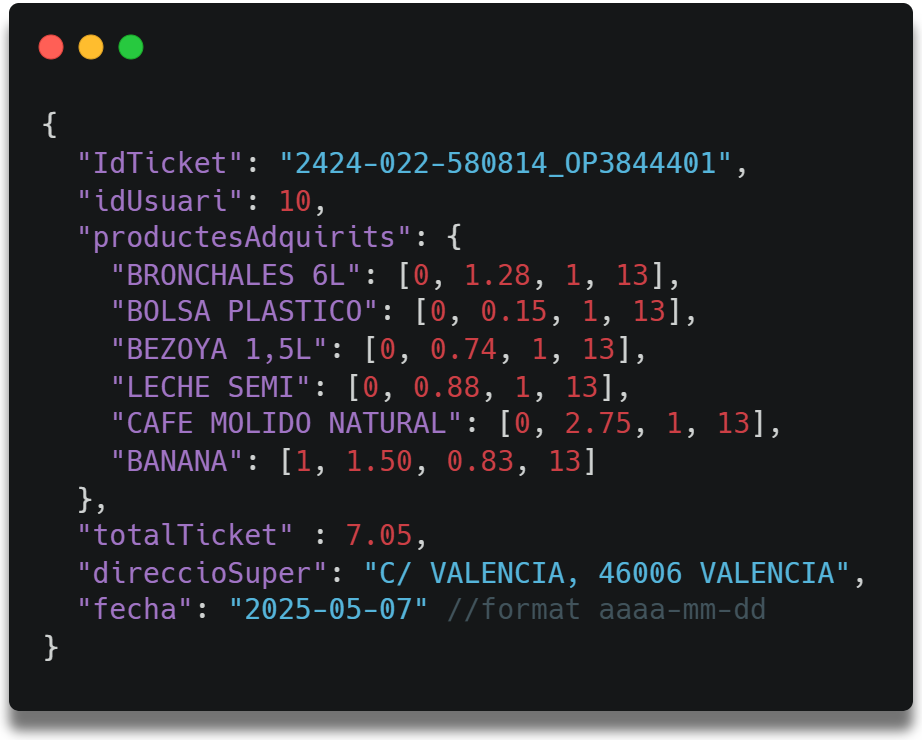
\includegraphics[width=.8\linewidth]{img/ticketJsonEstructuratMostra}
			\label{fig:ticketJsonEstructuratMostra}
		\end{figure}
		\FloatBarrier


		\FloatBarrier
		\setlength{\belowcaptionskip}{3pt}
		\begin{figure}[H]
			\centering
			\caption{Formato en el que parsearemos cada ticket digital de Mercadona para poder guardarlo en MongoDB y habilitar consultas eficientes formato con claves descriptivas por cada producto (items sin clasificar)}
			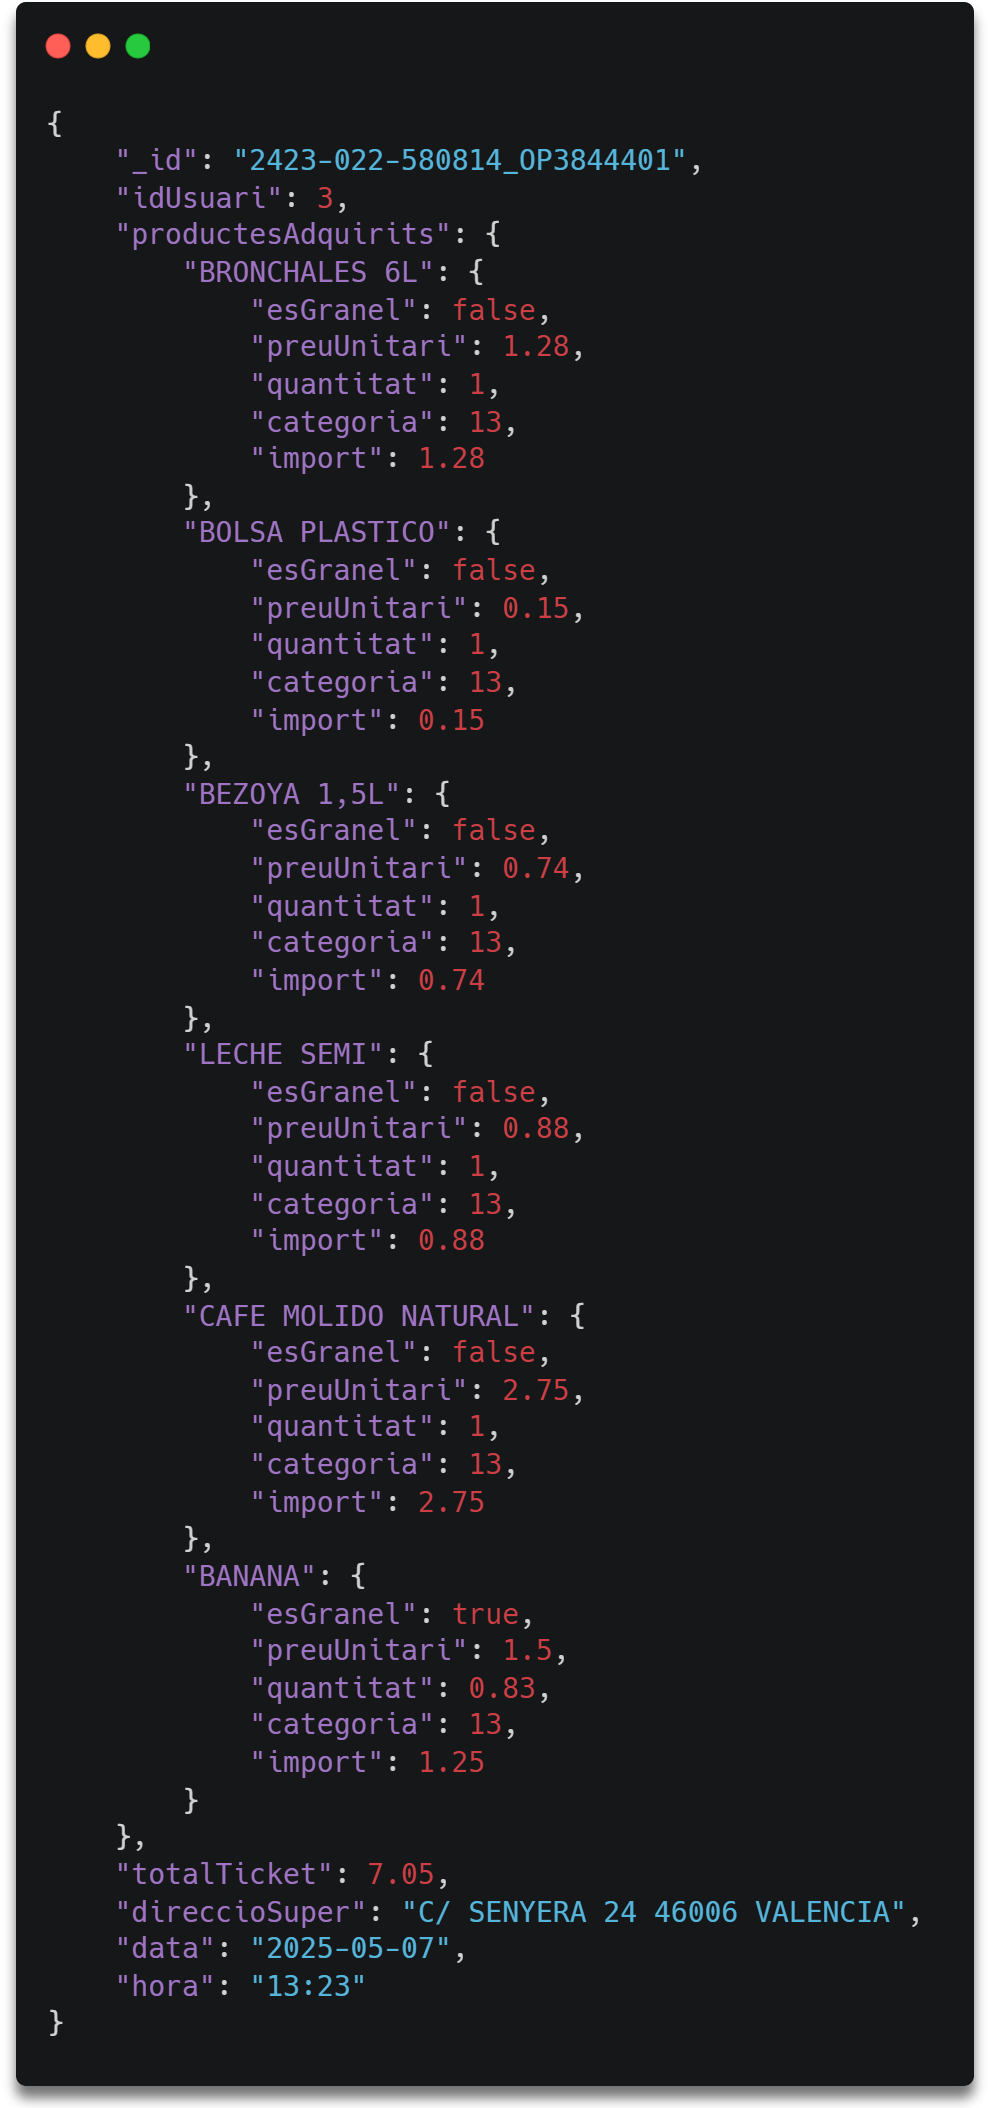
\includegraphics[width=.75\linewidth]{img/ticketJsonEstructuratMostraAMBCLAUS}
			\label{fig:ticketJsonEstructuratMostraAMBCLAUS}
		\end{figure}
		\FloatBarrier
		
		
	
		
		\subsubsection{PARTE 3: FastAPI manda a MongoDB los datos de los tickets parseados}
		\label{sec:PARTE3_FASTAPI}
		
		
		Mientas dura la llamada POST al endpoint \href{https://github.com/blackcub3s/mercApp/blob/f5413ed8cf7ed88c5ed18299564b836d27c52bd4/APP%20WEB/__FastAPI__/app/controlador.py#L132-L152}{/api/parsea-y-guarda-pdfs-en-bbdd}, que iniciamos en la PARTE 2, va a acontecer el guadado de los datos extraídos en el formato para poder hacer búsquedas eficientes en una base de datos NOSql: MongoDB, como vimos en la figura \ref{fig:ticketJsonEstructuratMostra}.
		
		Desde el algoritmo de extracción que ya hemos mencionado (\href{https://github.com/blackcub3s/mercApp/blob/main/APP%20WEB/__FastAPI__/app/serveiTickets.py}{serveiTickets.py}) podemos ver que hacemos llamada a funciones que residen en la capa de persistencia de nuestro back-end de FastAPI \href{https://github.com/blackcub3s/mercApp/blob/main/APP%20WEB/__FastAPI__/app/repositoriTickets.py}{repositoriTickets.py}, que es la responsable de guardar y extraer los datos hacia o desde MongoDB.
		
		\textbf{NOTA}: \textit{Este paso se puede alargar dependiendo del número de tickets que debamos procesar. Si se diese el caso el protocolo HTTP no nos serviría y deberíamos explorar otros caminos (Websockets, gPRC), porque el navegador podría no permitir tener una conexión abierta mucho tiempo; en el momento de la entrega del proyecto puede que hayamos tomado alguno de esos caminos alternativos -pero a ser posible se seguirá con protocolo HTTP por simplicidad-.}
		
		
		
		
		
		
		
		
		
		
		\subsubsection{PARTE 4: FastAPI manda el token de acceso (con permisos a 0) hacia Spring Boot, se actualiza permisos en bbdd mysql, y Spring Boot le manda de vuelta un nuevo token (con permisos a 1) a FastAPI}
		\label{sec:PARTE4_FASTAPI}
		
		Desde FastAPI, mientras todavía dura la solicitud HTTP a \textit{/api/parsea-y-guarda-pdfs-en-bbdd} que iniciamos en la PARTE 2, haremos ahora una llamada (como si fuese un cliente) hacia Spring Boot desde esta clase de servicio \href{https://github.com/blackcub3s/mercApp/blob/main/APP%20WEB/__FastAPI__/app/serveiClient.py}{serveiClient.py} usando el módulo \textit{httpx}. Si el token saliente de FastAPI se dictamina válido en Spring Boot, entonces este último framework actualizará la variable de permisos en la tabla Usuaris de la bbdd mySql cambiándolo de 0 a 1. Acto seguido, Spring Boot nos mandará de vuelta un nuevo token de acceso ``fresco'' con los permisos actualizados a 1. Al recibirlo en FastAPI se mandará la response al cliente (navegador) cerrando ya esa solicitud HTTP iniciada en la PARTE 2, que al recibirlo  (en \texttt{pas4\_concedirAccesGmail.html}) JavaScript dirigirá al dashboard en menos de un segundo y mostrará el dashboard de visualización.
		
		
	
	
	\subsection{Gestión de solicitudes: token de acceso}
	
	Con fastAPI no emitimos tokens de acceso: esto lo gestionamos con Spring Boot. Con FastAPI los recibimos del cliente y los procesamos\footnote{A excepción del caso especial de la PARTE 4!}: \textbf{si al hacerlo son válidos y no caducados, permitimos solicitudes entrantes.}
	
	Por ejemplo, en dos endpoints de FastAPI (``\textit{/api/subir-tickets-pdf}'' y ``\textit{/api/conta-pdfs-servidor}'') llamados desde \texttt{pas4\_concedirAccesGmail.html} en \href{https://github.com/blackcub3s/mercApp/blob/main/APP%20WEB/__FastAPI__/app/controlador.py}{controlador.py}  podemos ver esta línea:``\textit{payload\_token: dict = Depends(verificar\_token)}''
	 
	 Esta línea lo que está haciendo es llamar a la función verificar\_token en \href{https://github.com/blackcub3s/mercApp/blob/main/APP%20WEB/__FastAPI__/app/jwtUtil.py}{jwtUtils.py}. Este archivo Python, al que convenientemente le hemos puesto el mismo nombre que el que tenía la clase en Java (Spring Boot) donde guardábamos el secret con el que generábamos los tokens desde el otro back-end, no es casual: justamente aquí también guardamos una copia del mismo secret!
	
	Ese ``secret'' es indispensable para validar si el token entrante en cualquiera de los endpoints que tenemos es válido o no (i.e. no se ha manipulado y podemos certificar su origen como token expedido desde Spring Boot). Es por ello que se ha puesto por duplicado tanto en el back-end de FastAPI (Python) como en el back-end de Spring Boot (Java).
	
	Es importante mencionar que la gestión de tokens en Python (FastAPI) se hace notablemente más sencilla que con Java (Spring Boot). Por ejemplo, con FastAPI podemos conseguir que los endpoints no permitan solicitudes entrantes si el token ha caducado sin tener que gestionar la lógica de programación manualmente como sí teníamos que hacer con Spring Boot: en Spring Boot necesitábamos programar un total de 4 clases (dos clases para definir creación del token de acceso \href{https://github.com/blackcub3s/mercApp/blob/main/APP%20WEB/__springboot__produccio__/app/src/main/java/miApp/app/seguretat/jwt/AccessToken.java}{AccessToken.java} y lectura \href{https://github.com/blackcub3s/mercApp/blob/main/APP%20WEB/__springboot__produccio__/app/src/main/java/miApp/app/seguretat/jwt/JwtUtil.java}{JwtUtil.java}; otra clase para manejar las excepciones de un token expirado y forzar que solo usuarios con un cierto id puedan acceder a contenidos: \href{https://github.com/blackcub3s/mercApp/blob/main/APP%20WEB/__springboot__produccio__/app/src/main/java/miApp/app/seguretat/FiltreAutenticacioJwt.java}{FiltreAutenticacioJwt.java}; y finalmente una clase que defina un Bean que permita acceso a determinados endpoints a determinados usuarios según permisos, con la función requestMatchers: \href{https://github.com/blackcub3s/mercApp/blob/main/APP%20WEB/__springboot__produccio__/app/src/main/java/miApp/app/seguretat/ConfiguracioSeguretat.java}{ConfiguracioSeguretat.java}). Por el contrario, en FastAPI, con la librería de Python \textit{JOSE} \cite{pythonJose}\footnote{un nombre aparentemente muy español pero cuyo acrónimo significa \textit{JavaScript Object Signing and Encryption (JOSE)}} se hace todo muy rápido y solamente con las dos primeras funciones del archivo \href{https://github.com/blackcub3s/mercApp/blob/main/APP%20WEB/__FastAPI__/app/jwtUtil.py}{jwtUtil.py} lo hemos podido solventar.
	
	\subsection{Validación de datos (``/api/subir-tickets-pdf'')}
	\label{sec:validacioDadesApiSubirtickets}

	
	\FloatBarrier
	\setlength{\belowcaptionskip}{3pt}
	\begin{figure}[H]
		\centering
		\caption{Llamada al endpoint ``/api/subir-tickets-pdf'' $|$.\textbf{ Izq}: Solicitud POST con Postman: en verde, archivos que se suben correctamente; en rojo, archivos que servidor rechaza con las validaciones en FastAPI. $|$ \textbf{Der}: Solicitud POST con el navegador $|$ \textbf{Debajo}: PDFs subidos al sistema de archivos del servidor con FastAPI.}
		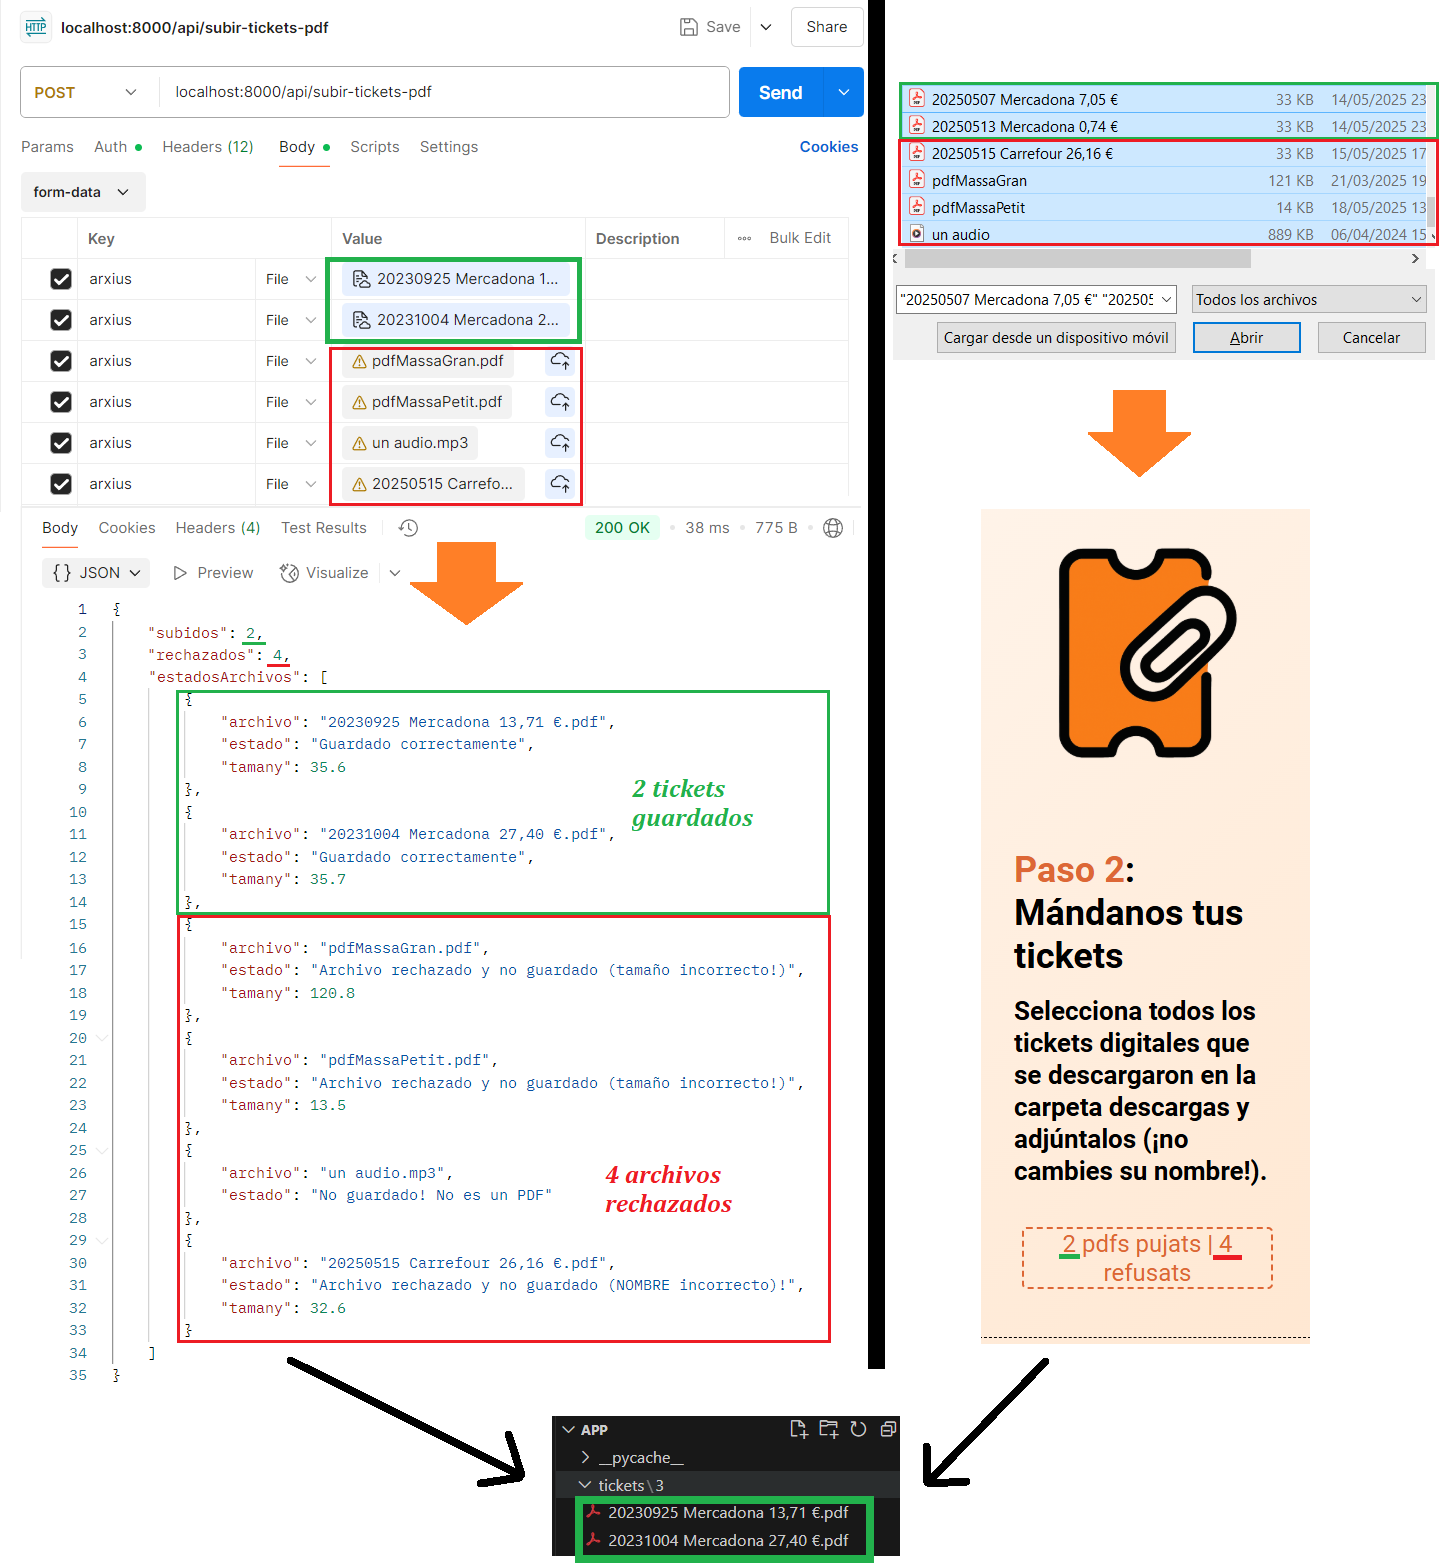
\includegraphics[width=1\linewidth]{img/validacionsArxiusPujadaEndpointTickets} 
		\label{fig:validacionsArxiusPujadaEndpointTickets}
	\end{figure}
	\FloatBarrier
	
	
	Al subir PDFs al sistema de archivos del servidor hemos tenido mucho cuidado, como vemos en la figura \ref{fig:validacionsArxiusPujadaEndpointTickets}.
	La validación de los datos se ha hecho antes de guardar los PDFs en el sistema de archivos del servidor, desde el lado del servidor (no desde el cliente); la solicitud al endpoint correspondiente del \href{https://github.com/blackcub3s/mercApp/blob/main/APP%20WEB/__FastAPI__/app/controlador.py}{controlador.py} activa una función de \href{https://github.com/blackcub3s/mercApp/blob/main/APP%20WEB/__FastAPI__/app/serveiValidacions.py}{serveiValidacions.py} que a su vez activa una función de \href{https://github.com/blackcub3s/mercApp/blob/main/APP%20WEB/__FastAPI__/app/serveiTickets.py}{serveiTickets.py}.
	
	Sabemos que será el usuario quien se descargue los tickets en pdf de su Gmail; pero luego, no podemos confiar que este sea responsable y suba archivos sin alterar al sistema de archivos de FastAPI. Por ende, se han verificado que se suban archivos en PDF (MIME type ``application/pdf'') como tipo de datos entrante. Luego, se ha mirado que los tamaños de los archivos estén comprendidos entre unos límites razonables, dado que cada Ticket digital de Mercadona ocupaba 36KB en 2023, reduciéndose a 33KB en 2025, podemos establecer unos intervalos razonables -un poco más amplios, pero no mucho más- para acomodar variaciones futuras que el supermercado pueda producir (véase detalle de líneas en \href{https://github.com/blackcub3s/mercApp/blob/23594665639485c1bf9b7ba7e1904fe9785cf5ae/APP%20WEB/__FastAPI__/app/serveiTickets.py#L84-L85}{este detalle} de serveiTickets.py) que a su vez nos protejan de uso malicioso de la API. En la función \textit{guardaTicketsAsistemaDarxius()} de  \href{https://github.com/blackcub3s/mercApp/blob/main/APP%20WEB/__FastAPI__/app/serveiTickets.py}{serveiTickets.py} tenemos en cuenta que no se cargue el archivo en memoria del servidor si es demasiado grande: así evitamos usos fraudulentos de la API. Si y solo si el archivo está entre los intervalos definidos, dejaremos que se lea en su totalidad y que luego se guarde.
	
	
	
	\section{Desarrollo del front-end}
	
	\subsection{Contenerización}
	\label{sec:conteneritzacioNginx}
	
	Se ha utilizado Nginx, un servidor de alto rendimiento para servir los archivos estáticos (HTML, CSS y JavaScript). Podéis ver su dockerfile \href{https://github.com/blackcub3s/mercApp/blob/main/APP%20WEB/__frontend__produccio__/Dockerfile}{aquí}, y el script que crea la imagen e instancia de contenedor \href{https://github.com/blackcub3s/mercApp/blob/main/APP%20WEB/__frontend__produccio__/creaImatge_i_arrancaContenidor.sh}{aquí}. Para más información del uso de Docker podéis ver el apartado \ref{sec:conteneritzacioPython} de la contenerización de Python.
	
	\subsection{Estructura de la aplicación}
	\label{sec:estructuraAplicacionFrontEnd}
	
	\FloatBarrier
	\setlength{\belowcaptionskip}{3pt}
	\begin{figure}[H]
		\centering
		\caption{Estructura de carpetas y archivos de la aplicación front-end: punto de entrada a la aplicación es index.html. Hay que abrir el proyecto con live server desde la carpeta app o si corremos el contenedor Docker de nginx moviéndonos al directorio donde está Dockerfile (moviéndonos a ../app) y derivar de él la imagen y el contenedor.}
		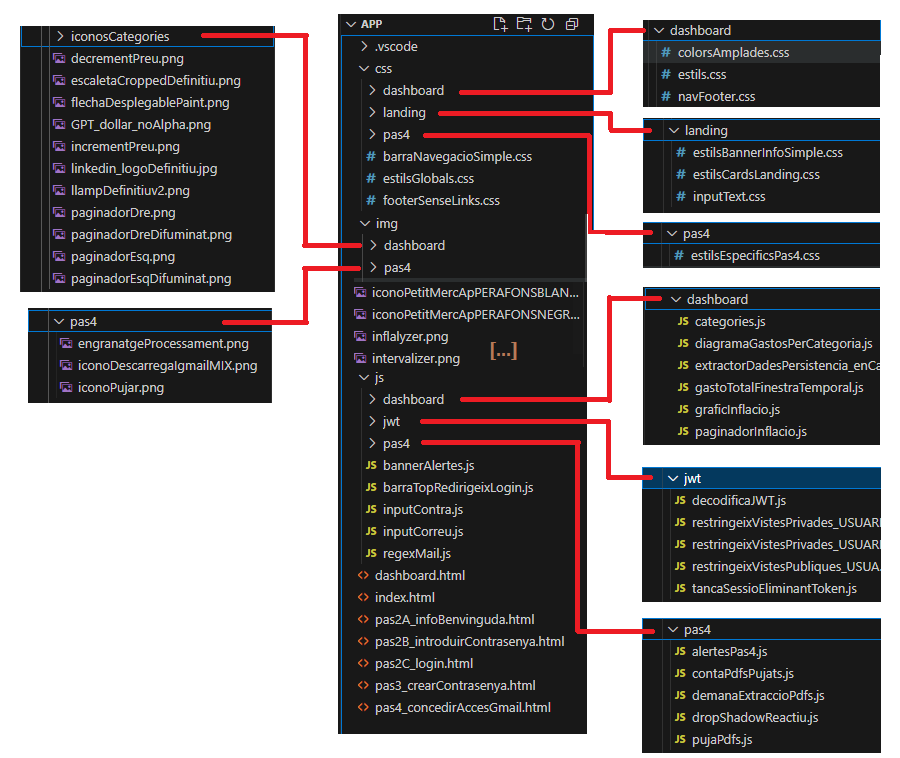
\includegraphics[width=1\linewidth]{img/estructuraAplicacioFront}
		\label{fig:estructuraAplicacioFront}
	\end{figure}
	\FloatBarrier
	
	
	
	
	\subsection{Enrutamiento de vistas}
	\label{sec:EnrutamientoDeVistas}
	
	Cuando un usuario introduzca su correo en el formulario de registro de la página principal de la web (\texttt{pas1\_LandingSignUp.html}, que renombraremos a \texttt{index.html}) va a ser redirigido con javascript a partir de las llamadas al back-end de Spring Boot: éste ultimo nos permitirá acceder al valor de la variable ``permisos'' de la tabla ``usuaris'' de mySql, siendo así redirigido a unas páginas u otras (el asunto de como se evita que ciertas páginas sean vistas por usuarios ya autenticados se cubre en otra sección: apartado \ref{sec:vistasPermisos}).
	
	

	
	Estas redirecciones no son fruto del azar. Se ha hecho un proceso de desarrollo inverso del proceso de registro de la plataforma NetFlix: replicándolo, desde cero, y adaptándolo a nuestro caso particular. Si Netflix utiliza ese esquema es porque tiene un impacto en la facilidad de captación de clientes y qué mejor que tratar de replicar los sistemas de los grandes \textit{players} (podéis ver anexo \ref{sec:annexNetflix} para más información).
	
	
	
	\setlength{\belowcaptionskip}{3pt}
	\FloatBarrier
	\begin{figure}[H]
		\centering
		\caption{\textbf{Imagen superior}: Detalle de la landing page \texttt{pas1\_LandingSignUp.html} (\texttt{index.html}) donde el usuario introducirá inicialmente su correo para registrarse -aunque ese mismo formulario en realidad nos servirá para todo gracias al enrutamiento de vistas- $||$ \textbf{Imagen inferior}: la página de Netflix en la que nos hemos inspirado para el diseño minimalista.}
		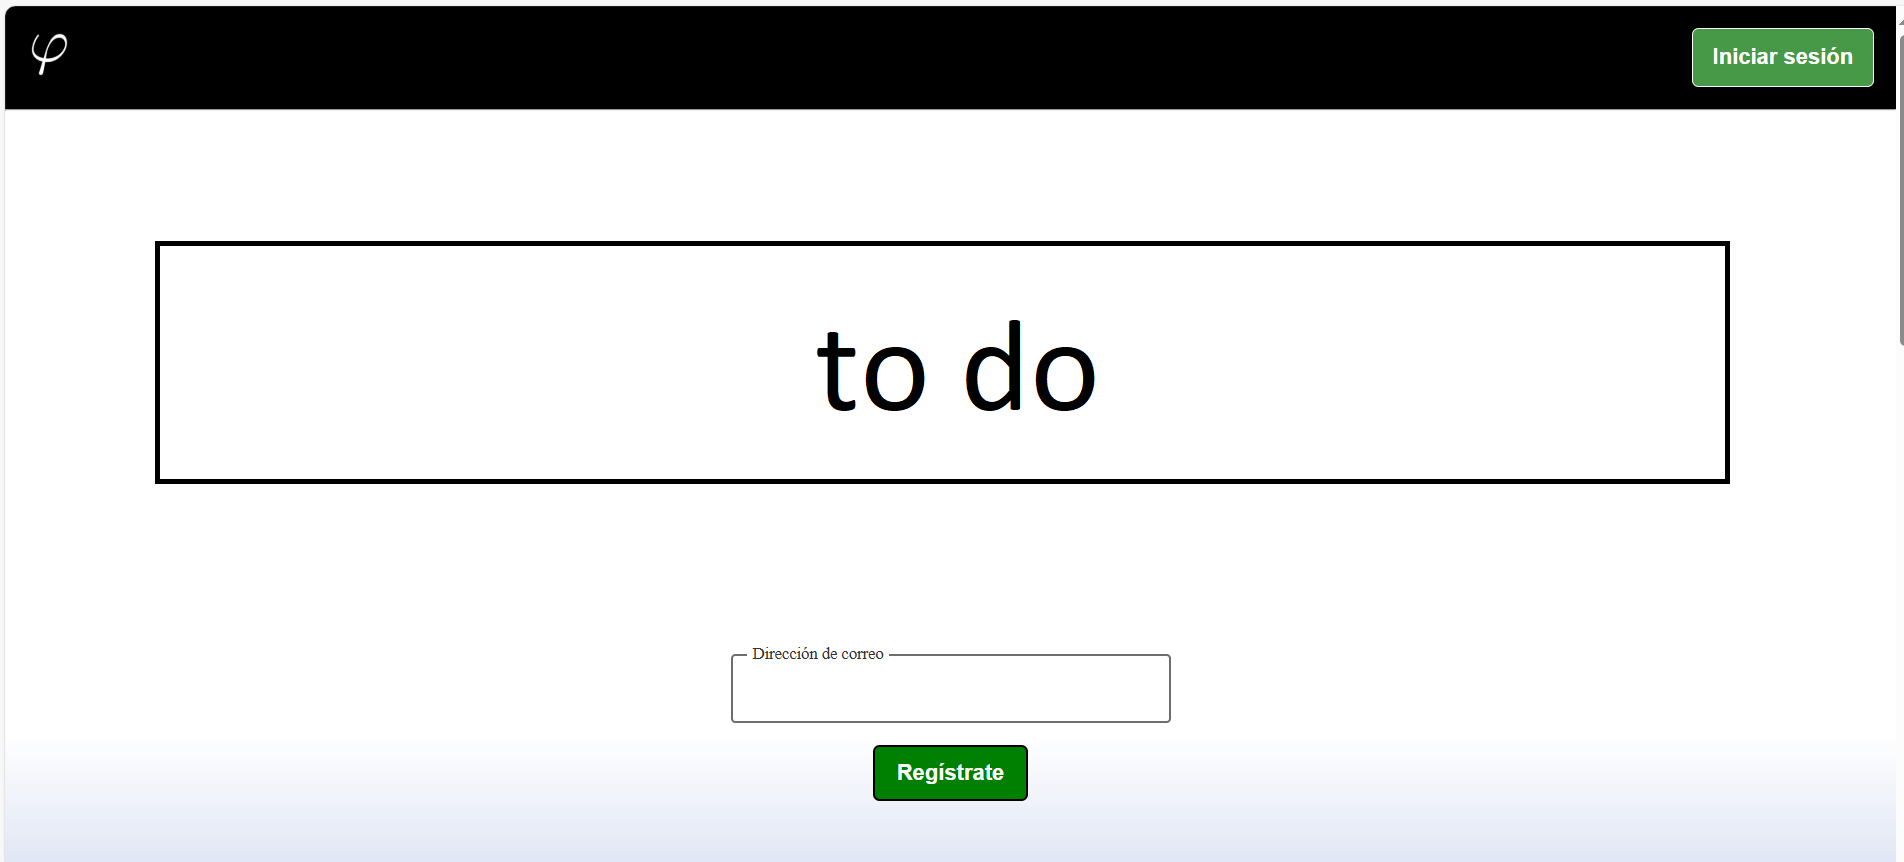
\includegraphics[width=1\textwidth]{img/landingSignUp.png}

		\label{fig:landingSignUpDETALL} 
	\end{figure}
	\FloatBarrier
	
	El esquema simplificado del proceso de enrutamiento durante el registro de un usuario en NetFlix queda recogido en el diagrama del anexo (ver apartado \ref{sec:anexo_diagramaNetflix}) y puede consultarse también en uno de los repositorios de mi github (\href{https://www.github.com/miApp}{link}). 
	
	Asimismo, el proceso de registro que utilizamos en mercApp es convenientemente una derivación de este mismo: si bien en NetFlix primeramente se redirige al usuario a unas cartas de pago, nosotros aquí le llevamos a una página para que nos dé acceso al gmail en el que Mercadona los tickets digitales al usuario (la página  \texttt{pas4\_ConcedirAccesGmail.html}); de nuevo análogamente a NetFlix, donde al usuario que ya ha pagado se le concede inmediatamente el acceso a las películas y series,  en nuestro caso se le dará acceso al usuario al tablón de visualización de análisis de datos de los tikets digitales  (\texttt{dashboard.html}), donde se visualizan el resultado de la minería y extracción de datos de esos tikets. 
	
	El proceso de enrutamiento de los usuarios desde que introducen el correo en el formulario de \texttt{pas1\_LandingSignUp.html} (\texttt{index.html}) hasta que acceden al \textit{dashboard} se encuentra recogido en el diagrama de la figura \ref{fig:diagramaMercaAppFront}. Para entenderla ver la pregunta siguiente:
	\vspace{1em}
	\hrule
	\textbf{¿Qué significan los distintos elementos visuales del diagrama de \ref{fig:diagramaMercaAppFront}?}
	\begin{itemize}
		\setlength{\itemsep}{-.3em}
		
		\item \textbf{\textcolor{taronjaBrillant}{\underline{rectángulos naranja}}}. $\rightarrow$ Representan las \underline{vistas} -archivos html- a las que redirige JavaScript mediante la llamada a $window.location.href$ a partir de los resultados de las llamadas a endpoint de APIs.
		\item \textbf{\textcolor{yellowfosforito!90!black}{\underline{rombos amarillos}}} $\rightarrow$ Representación de \underline{decisiones} del back-end de \textbf{Spring Boot} hechas como respuesta a peticiones de front-end a sus endpoints.%75 per cent groc fosforito i 25 negre entenc
		\item \textbf{\textcolor{blauCian}{\underline{rombo azul cian}}} $\rightarrow$ Una \underline{decisión} del back-end de \textbf{FastAPI} en respuesta a petición front-end a un endpoint de su API. 
		
		\item\textbf{\textcolor{green!70!white}{\underline{rectángulos verdes}}} $\rightarrow$ Representan \underline{expedición de tokens} de acceso (JWT) desde el endpoint del que emanan y su enviado a la vista a la que apuntan \footnote{Consultad la estructura de los mismos en la figura \ref{fig:jwtioMostraPayload}.}.
		
		\item Los endpoints de API que consume el front-end para hacer el enrutamiento se muestran entre corchetes ([]) y con colores. Concretamente tenemos:
		
		\begin{itemize}
			\setlength{\itemsep}{.0em}
			\item \textbf{\textcolor{red}{[\texttt{/api/avaluaUsuari}]}}: \textit{end-point} de Spring Boot que evalúa si el correo electrónico introducido pertenece a un usuario registrado y sus permisos.
			\item \textbf{\textcolor{brown}{[\texttt{/api/registraUsuari}]}}: \textit{end-point} de Spring Boot que registra un nuevo usuario en el sistema y expide su AccessToken con permisos a 0 en las \textit{claims} de su \textit{payload}\footnote{El lector puede consultar la explicación sobre lo que son las claims y el payload de un JWT en el apartado \ref{sec:queComponeJWTbackend}.}.
			\item \textbf{\textcolor{blue}{[\texttt{/api/login}]}}: \textit{end-point} de Spring Boot que gestiona el proceso de autenticación y generación del \textit{JWT Access Token} con tres niveles de permisos posibles (0, 1 y 2).
			\item\textbf{\textcolor{purple}{[\texttt{/api/parsea-y-guarda-pdfs-en-bbdd}]}}: \textit{end-point} de FastAPI que traslada al front-end AccessToken expedido por Spring B. con permisos a 1.
		\end{itemize}
		
				
		\item Finalmente debajo de los rectángulos naranja (vistas) hay un paréntesis del estilo (/dir1/dir2), sin color y pequeños. Estos paréntesis hacen referencia a las páginas o vistas de Netflix cuyo comportamiento replicamos -o hacemos corresponder en nuestra página- con vista o rectángulo naranja. Muy importante: véase anexo \ref{sec:annexNetflix}.
		
		

		

		

		
	\end{itemize}
	
	
	
	
	\setlength{\belowcaptionskip}{3pt}
	\FloatBarrier
	\begin{figure}[H]
		\centering
		\caption{Diagrama de flujo del enrutamiento completo del sistema \textit{front-end} durante el registro de un usuario, desde que este introduce su correo en \texttt{pas1\_LandingSignUp.html} (\texttt{index.html}) hasta obtener acceso al \texttt{dashboard}.\\ -------------------- \textit{NOTA:} \textbf{Acceso a recursos $\iff$ permisos $\geq$ 1} --------------------}
		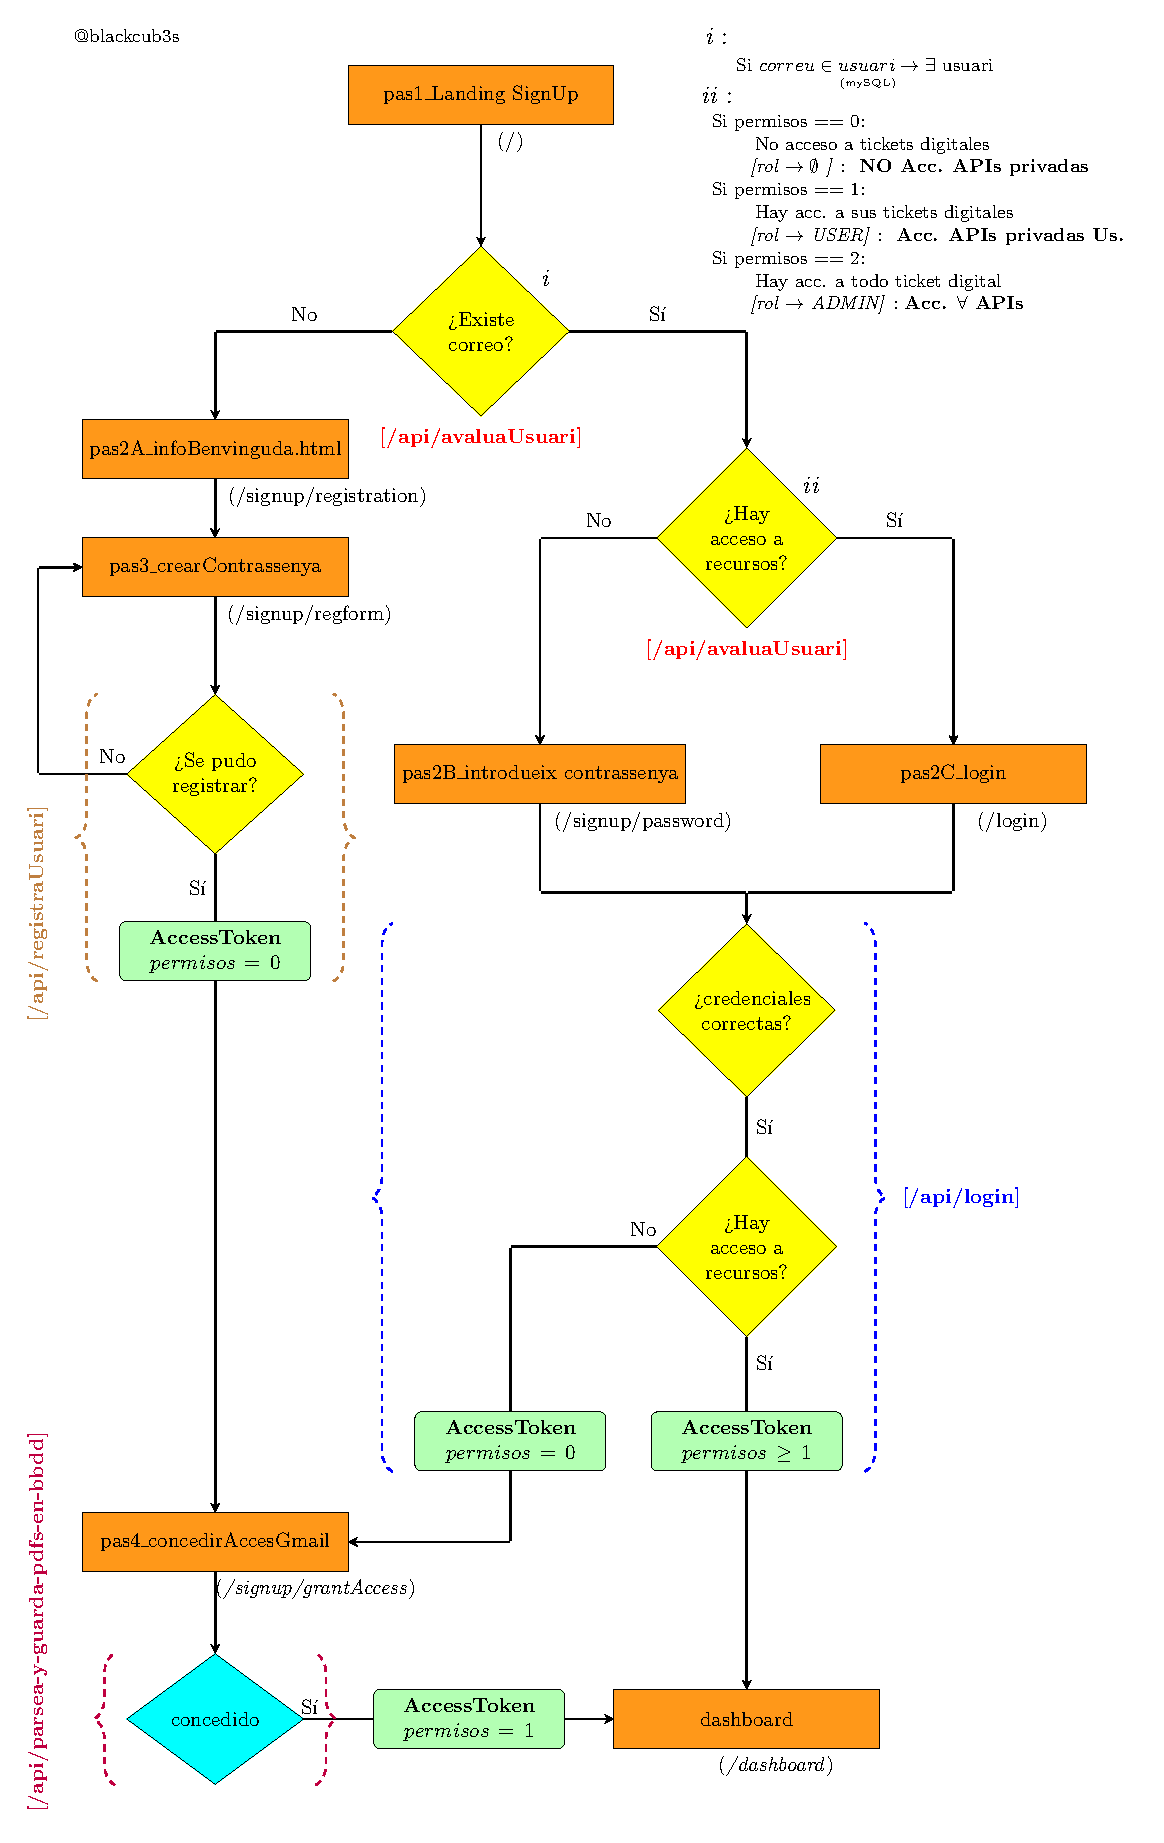
\includegraphics[width=1\textwidth]{img/diagramaMercAppFront.pdf}
		
		\label{fig:diagramaMercaAppFront} 
	\end{figure}
	\FloatBarrier
	
	
	
	
	
	
	
	
	\subsection{Manejar vistas en función de Autenticación y autorización}
	
	
	Como hemos visto antes Podemos considerar que cada archivo HTML y su CSS asociado es una ``vista'' de nuestra aplicación. Habrá vistas que \textbf{no nos interesará enseñar a ciertos usuarios}, porque o bien no serán relevantes para ellos o bien harán llamadas a APIs cuya información no podrá ser obtenida para ellos.
	
	Si bien Spring Boot permite servir los archivos estáticos\footnote{HTML, CSS y JS son archivos estáticos.}  de dentro del mismo back-end de Spring Boot y utilizar un sistema de plantillas (Thymeleaf) que permite impedir visualizaciones de vistas a usuarios no autorizados, esto realmente no es, para nada, lo ideal. Lo ideal es definir un front-end y un back-end separados partiendo de principios de \textit{separación de responsabilidades} o \textit{SoC}\footnote{Separation of concerns}, y así lo hemos hecho en este proyecto\footnote{Si tenemos ambas partes desacopladas podremos hacer modificaciones independientes en ambas. Por ejemplo, podremos cargar los archivos front-end en una CDN o un Proxy o tenerlos cacheados en un servidor que los sirva mucho más rápido, como Nginx. Es más, lo óptimo sería generar los archivos del front-end mediante un sistema de desarrollo por componentes (como Angular, React o Vue) para facilitar el desarrollo cuando la aplicación crezca y utilizar una paradigma \textit{SPA} (\textit{Single Page Application}). Sin embargo, en este caso, por el tiempo disponible y el tamaño de la aplicación se ha optado por hacerlo con HTML, CSS y JS puros.}. Las ventajas son grandes y tienen implicaciones en términos de mantenimiento, escalabilidad y reutilización tanto del front-end como del back-end (ver ventajas justificadas en anexo \ref{sec:SoCVENTATJES}).
	

	
	
	
	
	Sin embargo, no todo es ideal. Siempre existen concesiones (o como diríamos en inglés ``trade-offs''). Al tener el front-end y el back-end desacoplados esto también aumenta considerablemente la complejidad inicial en el desarrollo: la protección de las vistas a usuarios que no deben visualizarlas se hace más difícil porque no las sirve el back-end y no las puede proteger directamente este\footnote{A diferencia de lo que sí haría una aplicación back-end hecha en php tradicional como las que hemos visto en desarrollo web entorno servidor, donde servimos el HTML desde dentro del mismo PHP).}.
	
	Por ejemplo, del mismo modo que los endpoints de nuestra API del back-end en Spring Boot o del back-end de FastAPI están protegidos por token y no devuelven datos cuando el JWT de acceso que tengamos en el front-end haya caducado, sea inexistente, o sea inválido (porque haya sido manipulado o no tenga en el \textit{payload} el ``idUsuari'' que permita el acceso a un cierto recurso), también pasará que ciertas páginas del front-end no podrán obtener la información deseada si llaman a un end-point para el que no tienen autorización: en este caso ello tendrá implicaciones para las vistas, y deberemos modificar su DOM para la ocasión mostrando un mensaje de error, instando al usuario a iniciar sesión y/o bien redirigir al usuario a la página correcta, por ejemplo. Nosotros hemos optado por este último enfoque.
	
	Con tal de conseguirlo, deberemos manejar la lógica en cada caso particular desde el front-end usando JavaScript. Tengo entendido que en frameworks como Angular esto se puede hacer de forma muy sencilla, solo definiéndolo en una ocasión. Aquí cada página particular requerirá una programación específica con JavaScript para redirigir a los usuarios.
	
	\subsubsection{Protegiendo vistas ``privadas'' ante usuarios no ``logueados'': cuando el token ha expirado}
	
	Existen dos páginas de nuestra web que, cuando expire el token de acceso que se requiere para acceder a los recursos back-end que hay detrás de ellas (o este no exista), no deberán ser visualizables:
	
	\vspace{0em}
	\begin{itemize}
		\setlength{\itemsep}{-.5em}
		\item \texttt{pas4\_concedirAccesGmail.html}
		\item \texttt{dashboard.html}
	\end{itemize}
	
	Como se desprende del diagrama de flujo del enrutamiento del proceso de registro que vimos en la figura \ref{fig:diagramaMercaAppFront}, esas dos páginas son aquellas páginas de nuestro proyecto a las que redirigimos los usuarios justo después de generar tokens de acceso; por ende, su visionado requiere cierto grado de autenticación y autorización. De ahí que consideremos no permitir visualizarlas si el grado de permisos requerido no se llegase a satisfacer.
	
	La primera página (\texttt{dashboard.html}), requiere tener un token con permisos a 0; la segunda (\texttt{pas4\_concedirAccesGmail.html}) un token con permisos superior o igual a 1. En otras palabras: ambas requieren tener algún tipo de autenticación de usuario que se materialice en un token de acceso con una variable de permisos (i.e a esto nos referimos con usuarios ``logueados'' en el título), como veremos en el siguiente apartado; pero está claro que para visualizar cualquiera de estas dos páginas o vistas, la condición \textit{sine qua non} comuna es que dentro de \textit{localStorage.getItem(``AccessToken''}) se albergue un token de acceso que \underline{no esté expirado} y que sea \underline{descifrable}\footnote{Ojo, descrifrable no significa validable. Validable es lo que hacemos en el back-end con el secret, y no se muestra jamás en el cliente.}.
	
	Si está expirado, cuando hagamos la diferencia entre el valor ``exp'' del payload\footnote{Segundos en que el token expira o expiró, desde la epoch.} y la función \textit{Date.now()/1000}\footnote{Segundos actuales del navegador, desde la epoch.} saldrá un número negativo. En caso contrario, positivo. 
	
	Si el token está expirado -o es inexistente- inmediatamente redirigiremos al usuario a la landing page llamando a \textit{redirigeixAlandingPage()}, impidiendo así el visionado de cualquiera de las dos páginas (se cargará el script que contiene esta función antes de que se cargue el DOM\footnote{El lector puede hacer la prueba siguiente: si el token ha caducado o el usuario no se ha logueado, accediendo a \texttt{pas4\_concedirAccesGmail.htm} o a \texttt{dashboard.html} verá como automáticamente se produce una redirección a \texttt{pas1\_landingSignUp.html} (\texttt{index.html}); o si se ha logueado, abrir la consola y verá una cuenta atrás del tiempo que le queda al token de acceso para su expiración y para la redirección a la landing page.}). En cambio, si el token no está expirado seguiremos revaluando la expiración del token -y su existencia- con una frecuencia de un segundo: esto se conseguirá mediante la función asíncrona \textit{setInterval()} que hemos visto en desarrollo web entorno cliente de segundo curso.
	
	Para ello, en el \textit{head} de cada una de las dos páginas en cuestión veréis que \textbf{antes} siquiera \textbf{de cargar el DOM} se cargan sendos archivos:
	
\begin{lstlisting}[language=xml, basicstyle=\ttfamily\footnotesize, keywordstyle=\color{magenta}]
<script src="/js/jwt/decodificaJWT.js"></script>
<script src="/js/jwt/restringeixVistesPrivades_USUARI_NO_LOGUEJAT.js">
</script>
\end{lstlisting}


	
	En el primero tenemos la función para extraer el payload de un token. Y en el segundo está la lógica que acabamos de explicar en los párrafos anteriores (ver figura \ref{fig:restringeixVistesPrivades_USUARI_NO_LOGUEJAT}):
	
	
	\setlength{\belowcaptionskip}{3pt}
	\FloatBarrier
	\begin{figure}[H]
		\centering
		\caption{Script \texttt{restringeixVistesPrivades\_USUARI\_NO\_LOGUEJAT.js}, utilizado para regresar automáticamente a la landing page cuando el token de acceso de un usuario logueado expira -o es borrado- o cuando un usuario no logueado intenta acceder a las páginas que requieren permisos de acceso: \texttt{pas4\_concedirAccesGmail.html} y \texttt{dashboard.html}.}
		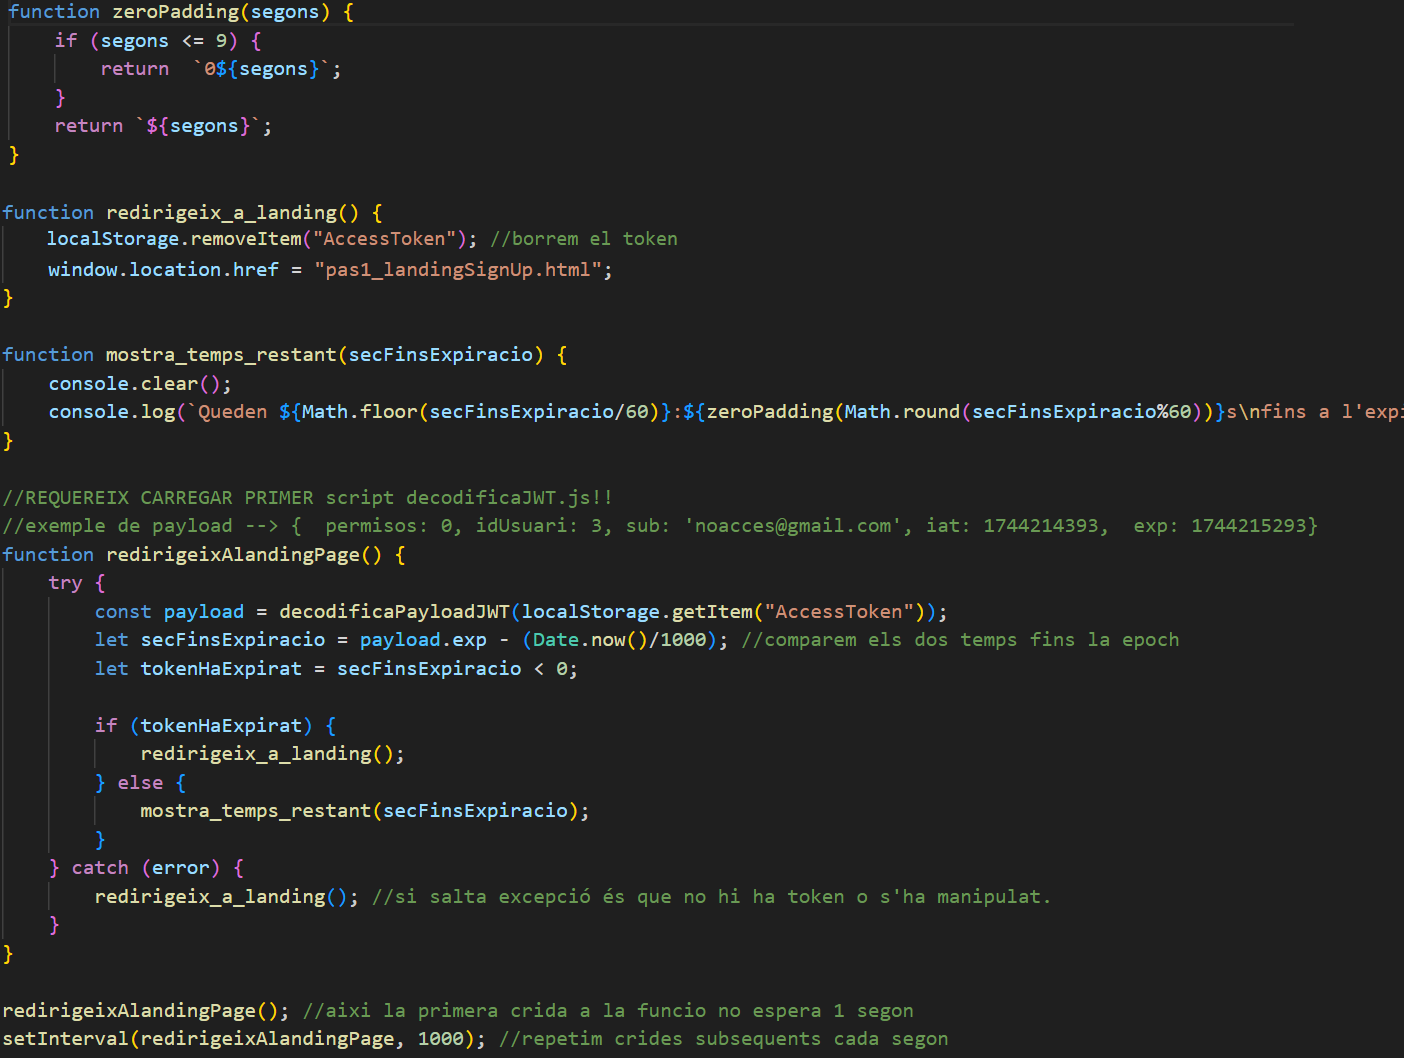
\includegraphics[width=1\linewidth]{img/restringeixVistesPrivades_USUARI_NO_LOGUEJAT.png}

		\label{fig:restringeixVistesPrivades_USUARI_NO_LOGUEJAT}
	\end{figure}
	\FloatBarrier
	
	\subsubsection{Protegiendo vistas ``públicas'' para usuarios ``logueados'': cuando el token no ha expirado}
	\label{sec:vistasPermisos}
	

	
	Para empezar, es necesario mencionar que se establecen tres niveles de permisos en la aplicación: estos  tienen un impacto sobre qué puede visualizar el usuario ``logueado'' y qué no; y cómo se permite que el usuario navegue a medida que va moviéndose en el proceso de registro cuando no está ``logueado''.
	
	Antes ya hemos visto que estos permisos nos han permitido construir el enrutamiento del front-end de la aplicación (su impacto podemos verlo en la parte superior derecha de la figura del enrutamiento \ref{fig:diagramaMercaAppFront} y más resumidamente en el cuadro \ref{table:permisos}), pero también ahora debemos utilizarlos también para \textbf{impedir} visualizar ciertas páginas en usuarios \underline{ya logueados}, es decir, aquellas páginas a las que nos referimos con el término ``vistas públicas'' empleado en el título de esta sección.
	
	\begin{table}[H]
		\centering
		\caption{Significado de la variable \texttt{permisos} en la tabla \texttt{usuaris} de mySQL.}
		\begin{tabular}{|c|l|}
			\hline
			\textbf{\texttt{permisos}} & \textbf{Significado} \\
			\hline
			0 & No hay acceso a tickets digitales (pero ya tenemos email y contraseña) \\
			1 & Acceso a tickets como usuario (USER) \\
			2 & Acceso a tickets como administrador (ADMIN) \\
			\hline
		\end{tabular}
		\label{table:permisos}
		
	\end{table}
	
	Programáticamente, debemos conseguir que estas ``vistas públicas'' \textbf{no sean visualizables} jamás si, en el \textit{local storage}, \textbf{existe}  un \underline{token de acceso} que \textbf{no haya expirado}\footnote{¡Si existe ese token no expirado significa que el usuario ya no debe acceder a ellas, porque ya se ha registrado y/o iniciado sesión y solo debe ver páginas de usuario registrado!}. Estas páginas vetadas a los usuarios ``logueados'' son las siguientes:
	
	\vspace{0em}
	\begin{itemize}
		\setlength{\itemsep}{-.5em}
		\item \textit{A)} \texttt{pas1\_landingSignUp.html} (\texttt{index.html})
		\item \textit{B)} \texttt{pas2A\_infoBenvinguda.html}
		\item \textit{C)} \texttt{pas2B\_introduirContrasenya.html}
		\item \textit{D)} \texttt{pas2C\_login.html}
		\item \textit{E)} \texttt{pas3\_crearContrasenya.html}
	\end{itemize}
	
	La forma que optamos para impedir su visualización es poner \textbf{dos scripts} en cada una de las cinco vistas públicas arriba mencionadas, que permitirán redirigir al usuario a la página ``privada'' que le corresponda según el valor que toma la variable ``permisos''\footnote{No hace falta mencionar que se saca del campo permisos de la tabla usuaris de la base de datos que tenemos en mySQL.} dentro del \textit{payload} del token de acceso guardado en el \textit{local storage} \footnote{Si queréis ver a qué me refiero con el payload, revisad de nuevo la figura \ref{fig:jwtioMostraPayload}.}, según se muestra en la tabla siguiente:
		
	\begin{table}[h!]
		\centering
		\begin{tabular}{|c|c|c|}
			\hline
			\textbf{página accedida} & \textbf{Permisos token} & \textbf{Redirigimos automáticamente a} \\
			\hline
			\multirow{2}{*}{\textit{A)}, \textit{B}, \textit{C)}, \textit{D)} o \textit{E)}} & $0$ & \texttt{pas4\_concedirAccesGmail.html} \\
			& $1 || 2$ & \texttt{dashboard.html} \\
			\hline
		\end{tabular}
	\end{table}

	En cada una de las páginas accedidas A), B), C), D) y E), antes que cargue el DOM, los dos scripts mencionados a cargar son:
	
\begin{lstlisting}[language=xml, basicstyle=\ttfamily\footnotesize, keywordstyle=\color{magenta}]
<script src="/js/jwt/decodificaJWT.js"></script>
<script src="/js/jwt/restringeixVistesPubliques_USUARI_LOGUEJAT.js"></script>
\end{lstlisting}

El segundo script, \texttt{restringeixVistesPubliques\_USUARI\_loguejat.js} es una modificación para la ocasión del script mostrado en la figura \ref{fig:restringeixVistesPrivades_USUARI_NO_LOGUEJAT} previa, y lo mostramos a continuación en la figura \ref{fig:restringeixVistesPubliquesUSUARILOGUEJAT}:


\setlength{\abovecaptionskip}{15pt}
\FloatBarrier
\begin{figure}[H]
	\centering
	\caption{Script \texttt{restringeixVistesPubliques\_USUARI\_LOGUEJAT.js}, utilizado para redirigir a un usuario logueado fuera de las páginas públicas de forma automática y directo a las 2 páginas posibles que requieren credencial de acceso (``privadas''), según proceda de acuerdo con la variable permisos de su token de acceso -si el token existe y no ha expirado-: \texttt{pas4\_concedirAccesGmail.html} y \texttt{dashboard.html}.}
	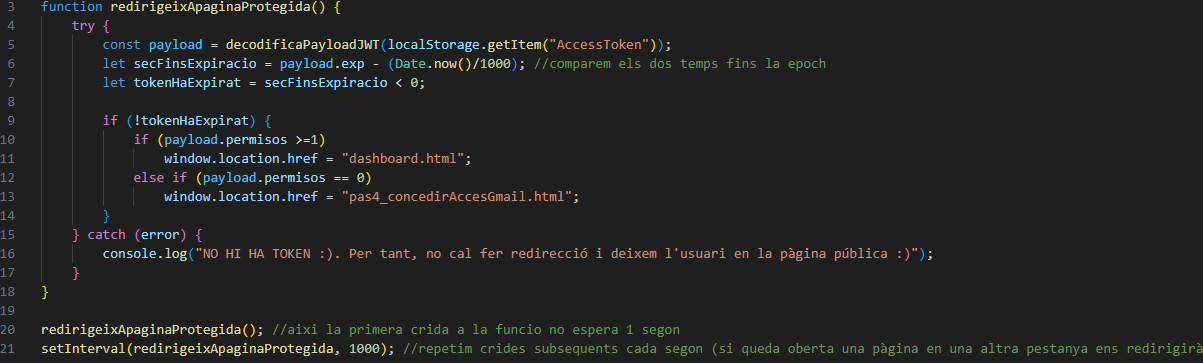
\includegraphics[width=1\linewidth]{img/restringeixVistesPubliques_USUARI_LOGUEJAT.png}
	
	\label{fig:restringeixVistesPubliquesUSUARILOGUEJAT}
\end{figure}
\FloatBarrier	
	


	
\subsubsection{Protegiendo vistas ``privadas'' ante usuarios ``logueados'': cuando el token no ha expirado.}
\label{sec:vistasPermisos}

Análogamente al apartado anterior, tenemos que tomar en consideración las páginas que requieren permisos de acceso. Estas páginas \textit{ya están} protegidas del visionado de usuarios no logueados (usarios que no tengan token expedido): estos no las podrán ver nunca, porque hicimos el script de la figura \ref{fig:restringeixVistesPrivades_USUARI_NO_LOGUEJAT} para redirigilos a la landing page en caso que por error accedan a ellas.

Sin embargo, nos queda algo por hacer: hay que conseguir \textbf{evitar} que un usuario con permisos 1 o 2 en el payload de su token (es decir, que ya ha concedido acceso a tickets digitales) pueda pedir de nuevo acceso a esos tikets; algo completamente innecesario porque ya los ha facilitado a mercApp previamente en \texttt{pas4\_concedirAccesGmail}; o, su opuesto: tenemos que evitar que un usuario con permisos 0 (e.g., ha puesto correo y contraseña y se ha registrado, pero no ha dado acceso a tickets digitales todavía) pueda tratar de visualizar el \texttt{dashboard} a la espera de obtener una información de unos tickets que él todavía no ha proporcionado.

La solución a lo anterior es hacer que en función de los permisos existentes en el token inhabilitemos una vista de las ``privadas'' para el usuario, \textit{mediante} la redirección automática del usuario a la página que sí debe visualizar \textit{antes} de que cargue el DOM de la pagina vetada, tal que así:
	
	\FloatBarrier
	\begin{table}[h!]
		\centering
		\begin{tabular}{|c|c|c|}
			\hline
			\textbf{p. privada accedida
				 (vetada)} &\textbf{Permisos} & \textbf{Redirección automática a} \\
			\hline
			\texttt{dashboard.html} & $0$ &  \texttt{pas4\_concedirAccesGmail.html}\\
			\texttt{pas4\_concedirAccesGmail.html} &$1 || 2$ & \texttt{dashboard.html} \\
			\hline
		\end{tabular}
	\end{table}
	\FloatBarrier

	
	Es decir, en la tabla anterior mostramos que si un usuario con permiso 0 (no ha concedido acceso a tickets digitales) quiere acceder a la página \texttt{dashboard.html} para visualizar la explotación de datos de los tickets, no podrá verla porque le redirigiremos automáticamente a la página donde podrá proporcionar acceso a tickets digitales: \texttt{pas4\_concedirAccesGmail.html}. Y viceversa: Si entra en \textit{pas4} teniendo permisos 1 o 2, será redirigido al \textit{dashboard}. 
	
	Lo que acabamos de mencionar en la última tabla y en el párrafo anterior lo programamos en el siguiente script (cuyo prerequisito será decodificaJWT como en las anteriores ocasiones) y que podemos ver en la imagen \ref{fig:restringeixVistesPrivadesUSUARINOLOGUEJAT}:
	
	
\begin{lstlisting}[language=xml, basicstyle=\ttfamily\footnotesize, keywordstyle=\color{magenta}]
<script src="/js/jwt/decodificaJWT.js"></script>
<script src="/js/jwt/restringeixVistesPrivades_USUARI_NO_LOGUEJAT.js">
</script>
\end{lstlisting} 
	
	
	\setlength{\abovecaptionskip}{15pt}
	\FloatBarrier
	\begin{figure}[H]
		\centering
		\caption{Script \texttt{restringeixVistesPrivades\_USUARI\_LOGUEJAT.js}, utilizado para redirigir a un usuario logueado hacia \texttt{pas4\_concedirAccesGmail.html} o \texttt{dashboard.html}, según proceda, en caso que el usuario entre en una de estas dos páginas privadas sin el permiso correspondiente.}
		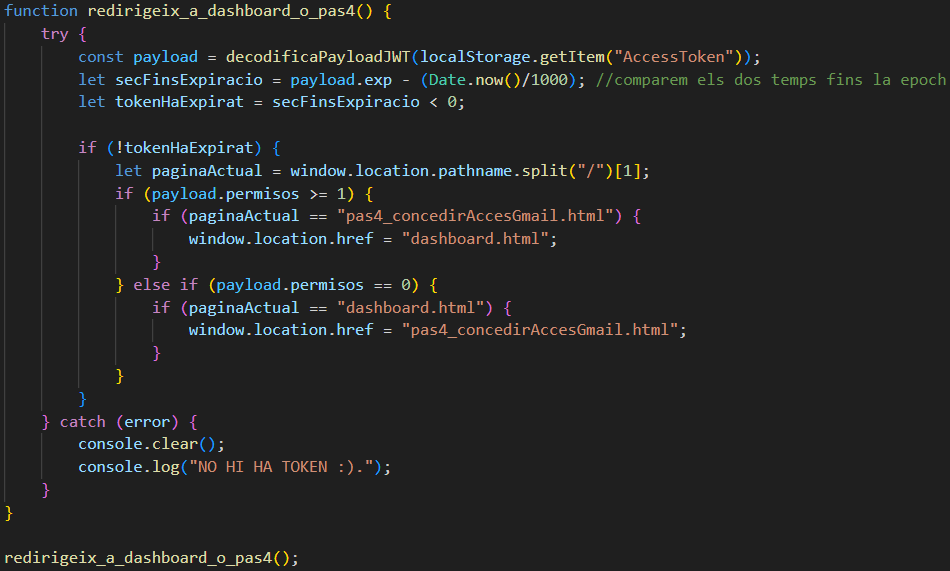
\includegraphics[width=1\linewidth]{img/restringeixVistesPrivadesUSUARINOLOGUEJAT.png}
		
		\label{fig:restringeixVistesPrivadesUSUARINOLOGUEJAT}
	\end{figure}
	\FloatBarrier	
	
	
	
	Para entender como guardamos los datos de permisos e ids de usuario en el front-end, podemos ver el apartado \ref{sec:recibirAccesTokenENFRONTEND} que viene a continuación, donde especificamos como se recibe el token del back-end y se guarda en el front-end.
	
	\subsubsection{Salir voluntariamente de las páginas privadas: botón ``cerrar sesión''}
	\label{sec:tancarSessioBotoExplicacio}
	
	El botón de ``cerrar sesión'' dentro de las dos páginas privadas \texttt{dashboard.html} y \texttt{pas4\_concedirAccesGmail.html} en realidad no cierra ninguna sesión. Recordemos que usamos token de acceso, que sustitye las sesiones. En el botón, sin embargo, hemos decidido mantener el nombre, porque el cierre de sesión es un concepto arraigado en los usuarios de sitios web, incluso más que el concepto de ``salir''\footnote{A nivel de usabilidad se me hace difícil justificar que un usuario diese click a un botón denominado ``eliminar token'' solamente porque el desarrollador quería ser preciso; dejemos esto como una prueba de como en ocasiones la usabilidad viene de la sencillez, no del honor a la verdad.}. 
	
	Lo que hace es , simplemente, eliminar el token de acceso del \textit{localStorage} cuando el usuario clica el botón de id ``botoEliminarToken''. 
	
	En cada una de estas páginas privadas recordemos que tenemos un script que cada segundo está reevaluando si hay token de acceso y si este es válido (ver script de figura \ref{fig:restringeixVistesPrivades_USUARI_NO_LOGUEJAT}). Por lo tanto, si lo borramos ese script va a redirigirnos a la página de inicio como máximo un segundo más tarde de la pulsación del botón de ``cierre de sesión''.
	
	\FloatBarrier
	\setlength{\abovecaptionskip}{15pt}
	\begin{figure}[H]
		\centering
		\caption{Script \texttt{tancaSessioEliminantToken} que elimina el token de acceso cuando el usuario clica en el botón ``cerrar sesión'' en las páginas privadas \texttt{dashboard.html} y \texttt{pas4\_concedirAccesGmail.html}}
		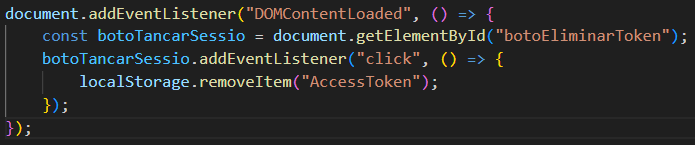
\includegraphics[width=1\linewidth]{img/scriptTancarSessio.png}
		\label{fig:scriptTancarSessio}
	\end{figure}
	\FloatBarrier
	
	
	
	\subsection{Recibir el Access Token desde el back-end}
	\label{sec:recibirAccesTokenENFRONTEND}
	
	Cuando un usuario del que ya tenemos su correo electrónico en BBDD intenta ``loguearse'' en mercApp\footnote{Sea que ya estuvo registrado -permisos 0-, dio acceso a sus tickets digitales -permisos 1- o es superusuario -permisos 2-.}, el token de acceso lo recibe por primera vez en el cliente cuando este haga una llamada fetch() hacia el endpoint del back-end ``\textit{/api/login}''. Esta llamada se hace desde \texttt{pas2C\_login.html} o desde \texttt{pas2B\_introdueix contrassenya.html}, de idéntica forma.
	
	
	Por ejemplo, explicaremos solamente el caso de \textit{pas2Clogin.html}. En este archivo la recepción del token se hará en el JavaScript embedido cuando, por un lado, obtengamos el código 200 (OK) del servidor; pero también, cuando se cumpla que el usuario y contraseña introducidos por el usuario son correctos. Si y solo si se cumplen ambas condiciones, el cliente entonces recibirá el token de acceso en el body de la respuesta a su solicitud, que será una como la que sigue, de la que podremos extraer el ``AccessToken'' y guardarlo inmediatamente en el LocalStorage del navegador: \footnote{Esto lo hacemos para luego poder mandarlo de vuelta al servidor en la subsecuentes solicitudes que requieran autenticación y autorización.} Para más información sobre el código JavaScript del front-end que lo permite véase figuras y \ref{fig:FetchCodisResponseFRONT} y \ref{fig:figuraLoginFetch}):
	
\begin{lstlisting}[language=Java, basicstyle=\ttfamily\footnotesize, keywordstyle=\color{magenta}]
	{
		"usuari": {
			"alies": "the protein kingdom",
			"permisos": 2,
			"idUsuari": 1
		},
		"existeixUsuari": true,
		"AccessToken": "eyJhbGciOiJIUzI1NiJ9.eyJwZXJ [...]",
		"teAccesArecursos": true,
		"contrasenyaCorrecta": true
	}
\end{lstlisting}
	

	
	\setlength{\belowcaptionskip}{3pt}
	\FloatBarrier
	\begin{figure}[H]
		\centering
		\caption{Fragmento de codigo en \texttt{pas2C\_login.html} dentro del codigo javascript para manejar codigos de error. Cuando el back-end de Spring Boot devuelve el código 200 significará que podremos extraer los datos del body de la respuesta. 400 se devolvería si hubiera problemas validación de campos en el back-end,  algo que no debería producirse nunca con el front-end que se ha programado.}
		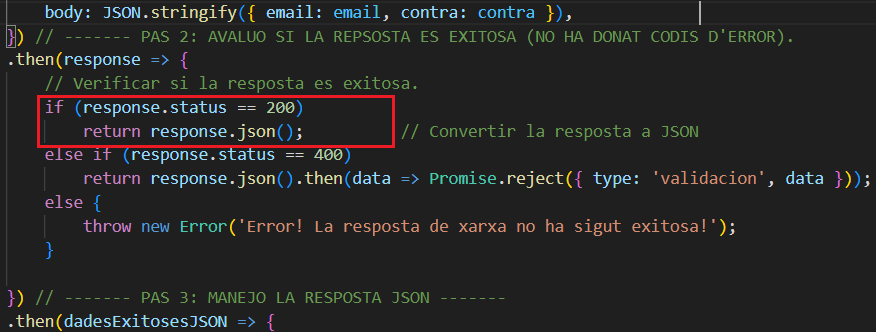
\includegraphics[width=1\textwidth]{img/FetchCodisResponseFRONT.png}
		
		\label{fig:FetchCodisResponseFRONT} 
	\end{figure}
	\FloatBarrier
	
	\setlength{\belowcaptionskip}{3pt}
	\FloatBarrier
	\begin{figure}[H]
		\centering
		\caption{Fragmento de codigo en pas2C\_login.html dentro del codigo javascript para obtener el token de acceso (detalle en rojo).}
		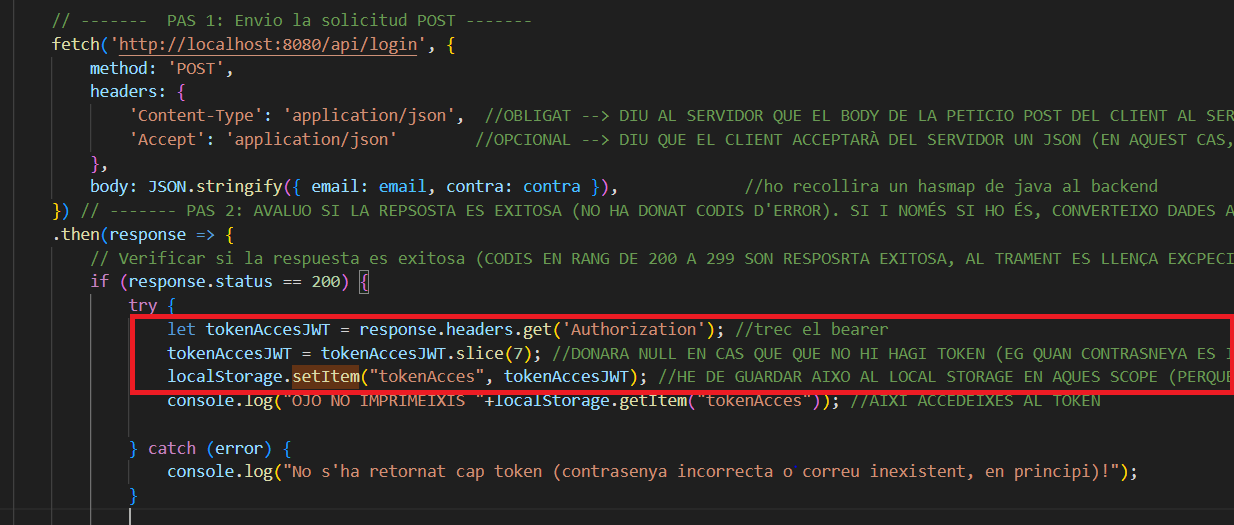
\includegraphics[width=1\textwidth]{img/jwtFetchLoginFront.png}
		
		\label{fig:figuraLoginFetch} 
	\end{figure}
	\FloatBarrier
	
	
	
	Ahora bien, si el usuario nunca se ha registrado en nuestra aplicación\footnote{Es decir, no tenemos su correo electrónico en BBDD.}, cuando lo haga, lo hará por el proceso de registro y no por el proceso de inicio de sesión. Una vez introduzca su contraseña en \texttt{pas3\_crearContrasenya.html} y se tome el correo electrónico insertado por el usuario en páginas previas y guardado en el localStorage, se hará una llamada POST con fetch() al endpoint ``api/registraUsuari'' pasando esos datos por el body: si y solo si el usuario NO existía, se creará un nuevo registro en la tabla Usuaris y ahi se devolverá un JSON con el token de acceso para el nuevo usuario creado, ahora de permisos 0. Este JSON tendrá el siguiente aspecto (el token será mucho más largo):
	
	
	
\begin{lstlisting}[language=Java, basicstyle=\ttfamily\footnotesize, keywordstyle=\color{magenta}]
{
	"existiaUsuari": false,
	"AccessToken": "eyJhbGciOiJIUzI1NiJ9.eyJw [...]",
	"usuariShaRegistrat": true
}
\end{lstlisting}
	
	
	Para entender de dónde viene el token desde el back-end redirigimos al lector a la sección \ref{sec:enviarPorPrimeraVezAccesTokenDESDEBACKEND}, donde se trata ese aspecto. En la presente sección nos ocuparemos de JavaScript en el front. Por ahora el lector debe tener claro que, como hemos visto ya, existen tres páginas HTML con códigos Javascript embedidos que pueden hacer llamadas asíncronas y obtener un token de acceso del servidor y guardarlo en el localStorage (un detalle de los formularios de estas páginas se encuentra en la figura \ref{fig:figPaginesQueExpedeixenJWT}):
	
	\setlength{\belowcaptionskip}{3pt}
	\FloatBarrier
	\begin{figure}[H]
		\centering
		\caption{Detalle de los formularios que permiten generar llamadas a los dos endpoints generadores de tokens de acceso (/api/login y /api/registraUsuari). De izquierda a derecha las páginas que los contienen: \texttt{pas2C\_login.html}, \texttt{pas3\_crearContrasenya.html} y \texttt{pas2B\_introduirContrasenya.html}}
		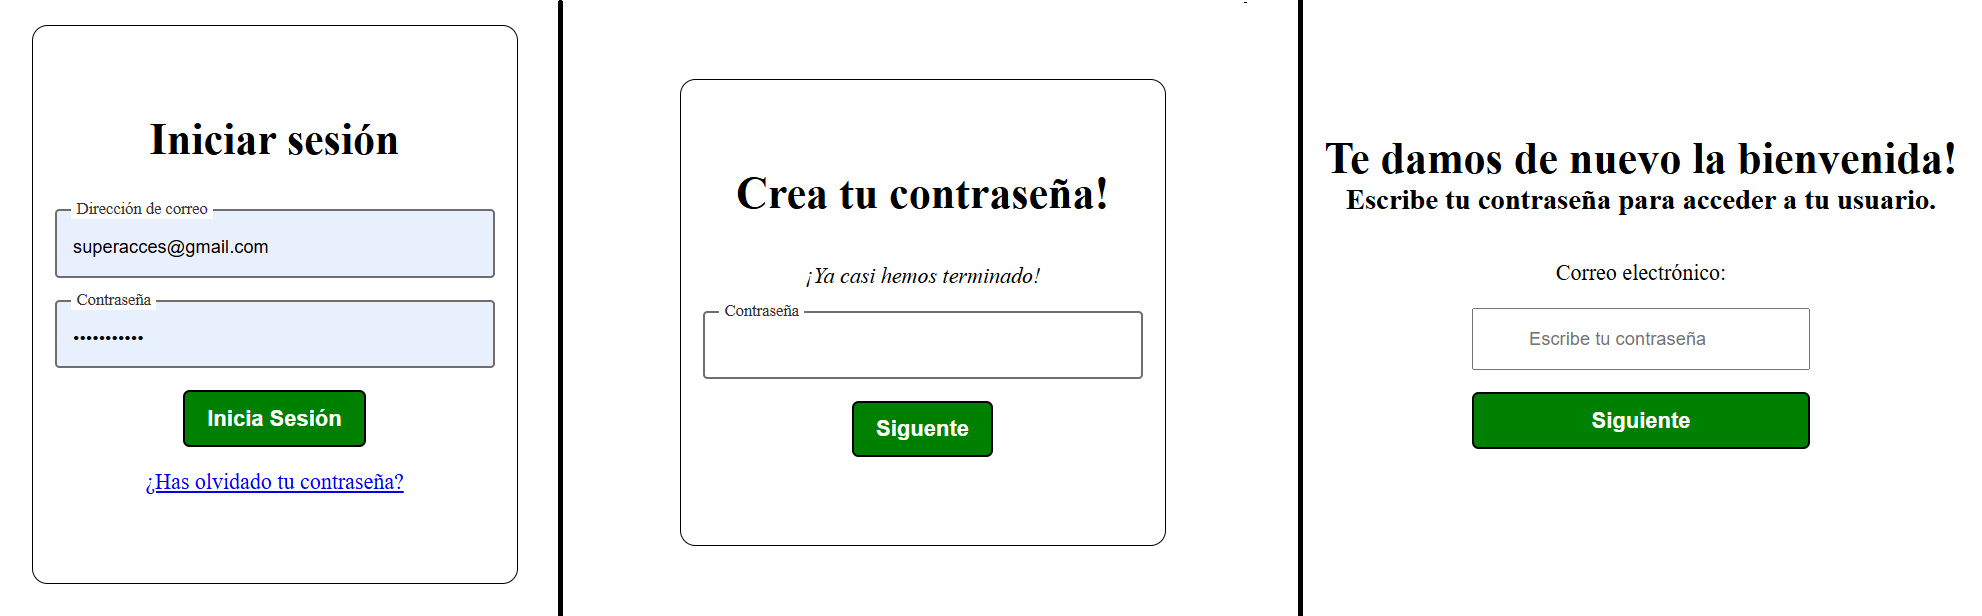
\includegraphics[width=1\textwidth]{img/figPaginesQueExpedeixenJWT.png}
		
		\label{fig:figPaginesQueExpedeixenJWT} 
	\end{figure}
	\FloatBarrier
	
	
	
\textit{NOTA: En este trabajo no implementaremos cookies ya que implica configuración extra tanto en el cliente como en el servidor. Vamos a guardar el token en el cliente en el localStorage (que es, de hecho, una práctica habitual en aplicaciones que no requieren un alto grado de seguridad). También hay que mencionar sobre que existe un debate para ver si en ese logIn el token de acceso recién generado en el servidor se debe mandar al cliente en el body de la respuesta de la solicitud POST \textit{o bien} en la header ``Authorization''. Sin embargo, es práctica común mandarlo en el body. Nótese, que para el paso inverso (cliente a servidor) sí debe mandarse en el Heather ``Authorization'' con el preámbulo ``Bearer '' seguido del token. }
	
	
	
	\subsection{Validación de datos (Formularios entrada)}
	\label{sec:validacioDadesFRONT}
	
	\textit{NOTA: Los datos validados en el front-end siguen las mismas expresiones regulares y restricciones que las validaciones hechas en el back-end (ver sección \ref{sec:validacioDadesBACK}) y establecen redundancia completa.}
	
	Vamos a poner el mismo caso concreto que pusimos en la sección homóloga de validaciones en el back-end de Spring Boot mencionado en el párrafo de la nota anterior. Asumamos también que un usuario quiere loguearse, pero no usando \textit{Postman} y llamando directamente al back-end sino a través del formulario que hay en nuestro front-end para el inicio de sesión.
	
	Para ello entra en la página \texttt{pas2C\_login} e introduce sus datos en el formulario que esta contiene (sin más complicación podéis ver el aspecto de este formulario en la figura anterior \ref{fig:figPaginesQueExpedeixenJWT}: es el que está a la izquierda).
	
	Con las validaciones aplicadas en el front nos impedirá llegar a mandar la solicitud POST (con fetch) al servidor si los datos introducidos no cumplen unos mínimos. Esto obedece a dos ventajas evidentes: la primera, es que el usuario obtiene feedback inmediato, porque es el cliente -navegador- el que gestiona los errores y no el servidor; la segunda, es que evitamos sobrecargar el servidor con procesos que se pueden gestionar perfectamente con el front.
	
	En este caso estas validaciones deben ser \textbf{exactas} a las validaciones del back-end, y solamente son un complemento y no las sustituyen, como ya hemos dicho en el apartado homólogo dedicado al back-end: deben tener correspondiencia completa con las validaciones del back-end porque si no están bien hechas en el front-end podría darse el caso que un usuario intentase poner unos datos que luego el back-end no admitiese o viceversa; además, no las sustituyen porque justamente un usuario puede modificar fácilmente el front-end, quitar las protecciones del javascript (bastaría quitar con el \textit{inspector} del navegador las llamadas a funciones de validación en dos líneas del javascript (\href{https://github.com/blackcub3s/mercApp/blob/d848aa27c1e460dc54bb665e9091d83e4b614531/APP%20WEB/__frontend__produccio__/app/pas2C_login.html#L31-L32}{éstas}) y entonces hacer llamadas directas a la API del back-end de Spring-Boot con la función fetch ya disponible para el usuario (\href{https://github.com/blackcub3s/mercApp/blob/d848aa27c1e460dc54bb665e9091d83e4b614531/APP%20WEB/__frontend__produccio__/app/pas2C_login.html#L36C31-L36C63}{detalle líneas}). Entonces, el endpoint \textit{/api/login} al que llamamos con la función fetch estaría desprotegido. A continuacón mostramos como validacmos el correo y la contraseña en el front:
	
		\subsubsection{Validación del correo}
	
		Cuando el usuario se loguea, es la función \textit{correuApte(email)} del archivo \href{https://github.com/blackcub3s/mercApp/blob/d848aa27c1e460dc54bb665e9091d83e4b614531/APP%20WEB/__frontend__produccio__/app/js/regexMail.js}{js/regexMail.js} la que valida la entrada de datos con una expresión regular. Podéis ver ese mismo archivo en la figura \ref{fig:regexMail}. 
		
		Para hablar de lo que hace esa expresión regular, vale la pena mencionar primero las de las que se compone un correo:
		
		\begin{lstlisting}[language=xml, basicstyle=\ttfamily\small]
		partelocal@dominio.subdominio
		\end{lstlisting}
		

		
		Con esa expresión regular se han permitido mayúsculas, minúsculas y ciertos caracteres como el +, el ampersand o el guión medio antes de la arroba (parte local). Después de la arroba de un correo introducido, se restringe de forma distinta el dominio y el subdominio: por ejemplo, el dominio no tiene restricción de longitud, pero el subdominio sí (debe tener más de 2 y menos de 7 caracteres). Nótese que esta misma expresión regular evita los caracteres peligrosos también (que igualmente protegería nuestro back-end): las ``'', los $<$ y $>$.
		
		\FloatBarrier
		\setlength{\belowcaptionskip}{0pt}
		\begin{figure}[H]
			\centering
			\caption[Detalle de validación del correo (js/regexMail.js)]{Mediante una sola expresión regular facilitada por un LLM hemos podido hacer una correspondencia completa con las validaciones del back-end.}
			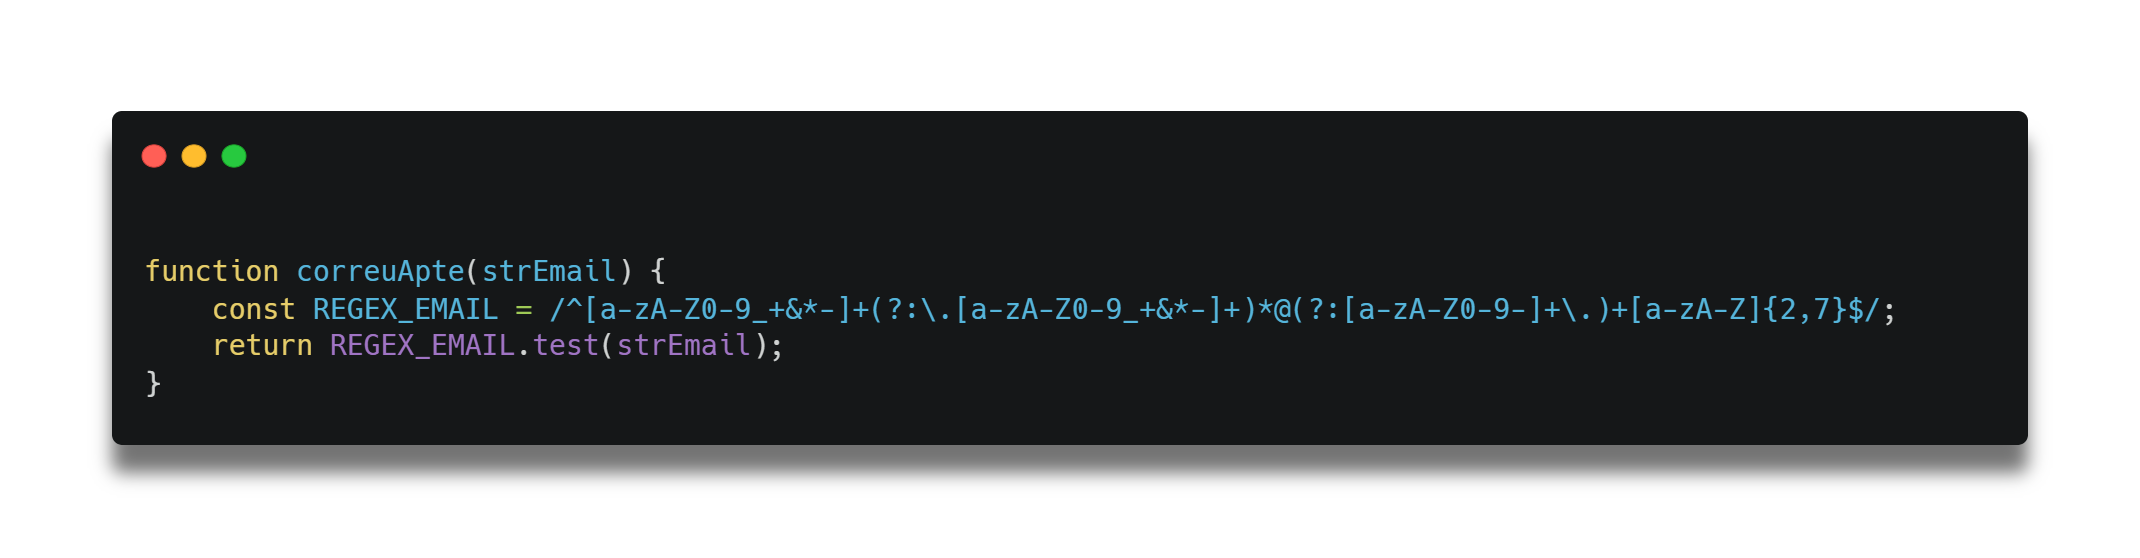
\includegraphics[width=1\linewidth]{img/regexMail}
			\label{fig:regexMail}
		\end{figure}
		\FloatBarrier
	
	
		Por ello, cuando un usuario ponga su correo en el formulario correspondiente de la vista de inicio de sesión en \texttt{pas2C\_login.html}, al \textit{darle a enviar} se va a activar en última instancia la función \textit{correuApte()} y saltará una alerta que impedirá que pueda mandar el correo si la expresión regular no se cumple. La alerta la llamaremos dentro del script embedido en el html de la propia página, y va a llamar a las funciones que generan banners de alerta que usaremos solamente en las páginas públicas (ubicadas en \href{https://github.com/blackcub3s/mercApp/blob/main/APP%20WEB/__frontend__produccio__/app/js/bannerAlertes.js}{js/bannerAlertes.js}) tal como podemos ver en la figura \ref{fig:activacioBannerAlertesLoginCorreu}.
		
		Asimismo, no en la página de login, pero sí en la página del formulario de registro (\texttt{index.html} o \texttt{pas1}) usamos esta misma función \textit{correuApte(email)} para generar información dinámica de los errores al usuario \textbf{antes} de que trate de enviar nada con el botón de registro. Esto lo hacemos mediante el uso de los eventos ``focus'', ``input'' y ``blur'' ampliamente vistos en la asignatura desarrollo web entorno Cliente de segundo de DAW (véase función \textit{esdevenimentsCorreu\_SIGN\_UP()} dentro del archivo de GitHub \href{https://github.com/blackcub3s/mercApp/blob/main/APP%20WEB/__frontend__produccio__/app/js/inputCorreu.js}{/js/inputCorreu.js}) para poder ver cómo se han conseguido los efectos en el contorno del formulario de registro para el correo del \texttt{index.html} ver la figura \ref{fig:logicaInputBlurSignup}. En esta figura explicamos el impacto que estos 3 eventos de JavaScript ayudan a mostrar prevalidaciones al usuario de una forma intuitiva. Los colores del contorno y los mensajes van en línea a como definen el feedback los formularios de correo de Google y de Netflix.
		
		\FloatBarrier
		\setlength{\belowcaptionskip}{3pt}
		\begin{figure}[H]
			\centering
			\caption{Activación del banner de alertas en el formulario de inicio de sesión de la vista \texttt{pas2C\_login.html} ante un input de correo incorrecto después de clicar en inicia sesión. ¡En este caso no se manda nada al servidor!}
			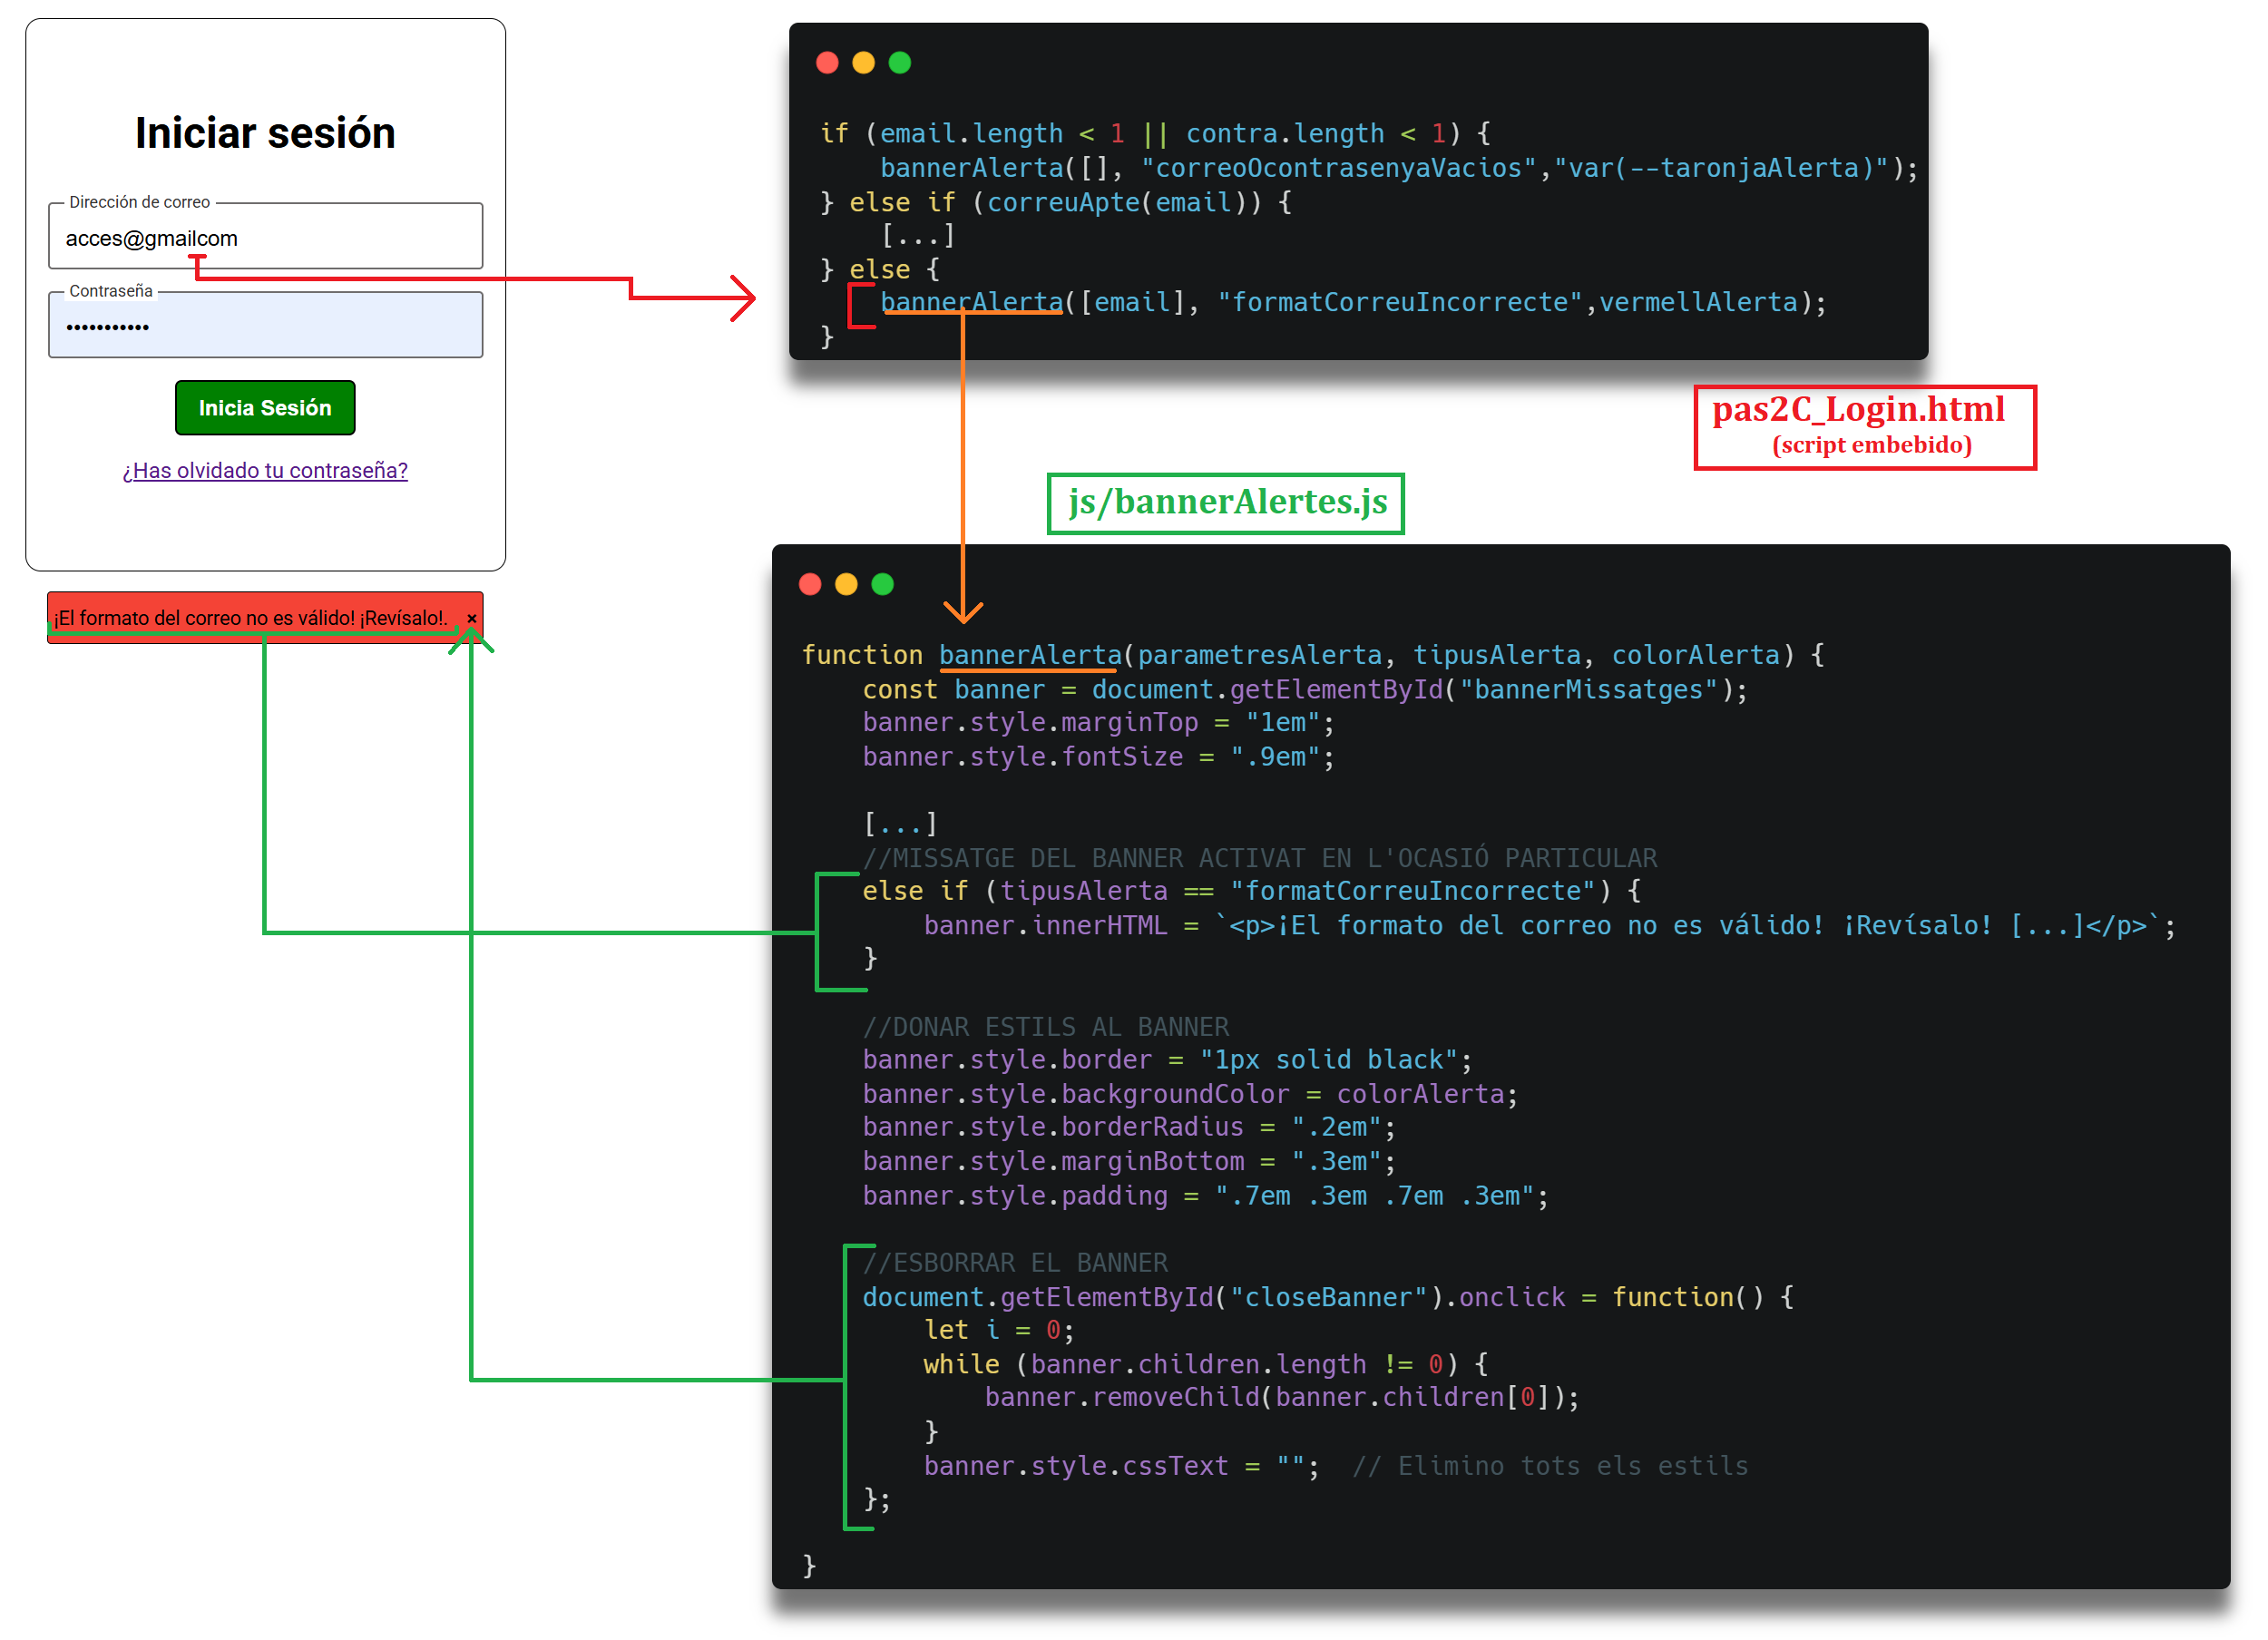
\includegraphics[width=.8\linewidth]{img/activacioBannerAlertesLoginCorreu}
			\label{fig:activacioBannerAlertesLoginCorreu}
		\end{figure}
		\FloatBarrier
		
	
	
		
		
		\FloatBarrier
		\setlength{\belowcaptionskip}{3pt}
		\begin{figure}[H]
			\centering
			\caption{Prevalidaciones en tiempo real en \texttt{pas1\_Landing SignUp} o \texttt{index.html}. $|$ \textbf{SupIzq}: estado natural (contorno gris)$|$ \textbf{SupDer}: click encima del formulario sin datos (cambio ante evento ``focus'', contorno azul)$|$ \textbf{InfIzq}: datos introducidos incorrectos (cambio ante evento ``blur'') $|$ \textbf{InfDer}: contorno muestra éxito con un correo válido (evento input, contorno a verde).}
			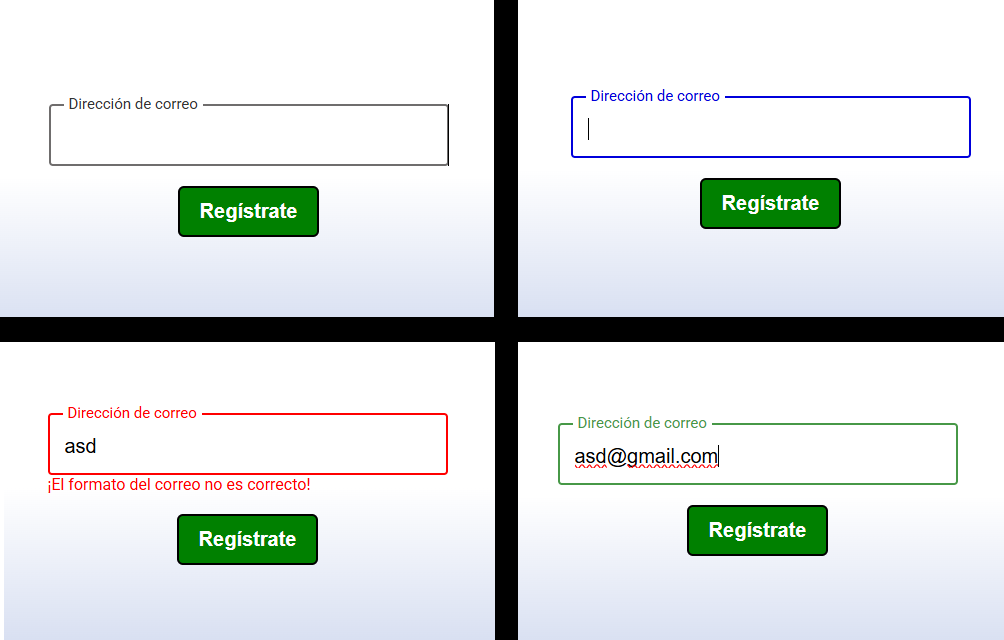
\includegraphics[width=.9\linewidth]{img/logicaInputBlurSignup}
			\label{fig:logicaInputBlurSignup}
		\end{figure}
		\FloatBarrier
		
		
		\subsubsection{Validación de la contraseña}
		
		La validación de la contraseña tanto en la página general de inicio de sesión \textit{pas2C\_login.html} como en la página pensada para aquellos usuarios que ya se registraron en nuestro sistema pero todavía no llegaron a obtener acceso al dashboard  \textit{pas2B\_introduirContrasenya.html} siempre la hacemos \textbf{después} de que el usuario haga click en el botón de iniciar sesión: si la contraseña no cumple los mínimos no se mandará nada al servidor. Estas validaciones (o post-validaciones, a lo mejor, sería mejor término) las hacemos sin usar eventos que se activen antes del evento click (a excepción del uso de ``focus'' y ``blur'', pero no para validar, sino para cambiar el contorno a azul cuando se hace click en el formulario: \href{https://github.com/blackcub3s/mercApp/blob/dc4941c33c65fb9133f4aa8ca890059243bf080d/APP%20WEB/__frontend__produccio__/app/js/inputContra.js#L45-L83}{ver detalle} de líneas de código).
		
		Estos mínimos de los que hablamos permiten verificar que el usuario esté entrando una contraseña que luego las validaciones del back-end también admitan. Estos mínimos los hemos generado verificando expresiones regulares con la función \textit{regex.test(contraseña)} vista en desarrollo web entorno cliente, que nos devuelve un booleano que indica si la \textit{regex} hace \textit{match} con la contraseña pasada por parámetro. Así las cosas, tomando diversas funciones \textit{.test()} aplicadas al binomio ``contraseña introducida - expresión regular'', podemos hacer la intersección de todas ellas mediante la operación lógica AND, como podéis ver en la figura \ref{fig:contrasenyaValidacioExprRegulars}, testeando así si la contraseña introducida es válida o no. Podéis ver el archivo completo \href{https://github.com/blackcub3s/mercApp/blob/main/APP%20WEB/__frontend__produccio__/app/js/inputContra.js}{/js/inputContra.js}
		
		
		\FloatBarrier
		\setlength{\belowcaptionskip}{3pt}
		\begin{figure}[H]
			\centering
			\caption{Subconjunto de código de \textit{js/inputContra.js} responsable de las validaciones de contraseña. Hemos querido apostar por obligar al usuario a generar una contraseña segura con mínimo una mayúscula, una minúscula, un número y sin espacios: forzando que no se puedan usar caracteres distintos a los grupos anteriores exceptuando el punto y la barra baja. También permitimos acentos y cedilla (ç).}
			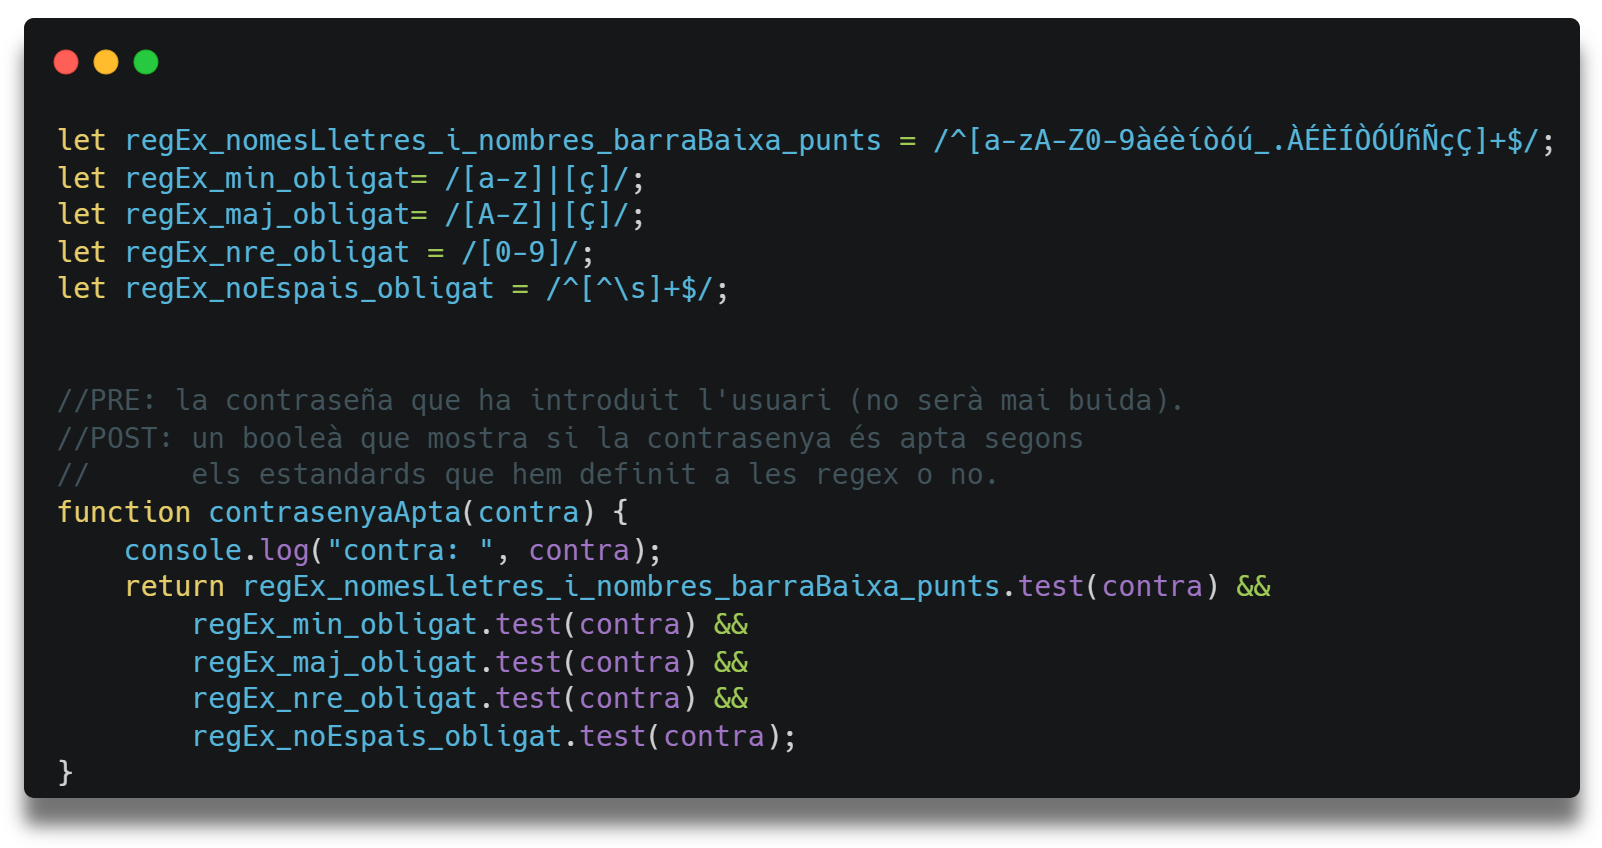
\includegraphics[width=.7\linewidth]{img/contrasenyaValidacioExprRegulars}
			\label{fig:contrasenyaValidacioExprRegulars}
		\end{figure}
		\FloatBarrier
		
		
		
		
		Un ejemplo de puesta en escena de las expresiones regulares de la figura anterior la podemos ver en la figura \ref{fig:activacioBannerAlertesLoginContrasenya} siguiente:
	
		
		\FloatBarrier
		\setlength{\belowcaptionskip}{3pt}
		\begin{figure}[H]
			\centering
			\caption{Hasta que la contraseña no reúne unos mínimos no se permite mandar nada desde el formulario de inicio de sesión hacia el servidor. Se muestra una relación de los archivos (scripts simplificados) y del recorrido de una contraseña erróneamente escogida e introducida en el formulario, que hacen posible mostrar el array de errores en pantalla vinculados con el formato incorrecto de la contraseña. Así el usuario tiene feedback y puede fácilmente ajustar la contraseña para que sea válida, dado que cada error emana de una expresión regular de las mostradas en la figura anterior. Nótese que seguimos sin hacer ninguna llamada al servidor.}
			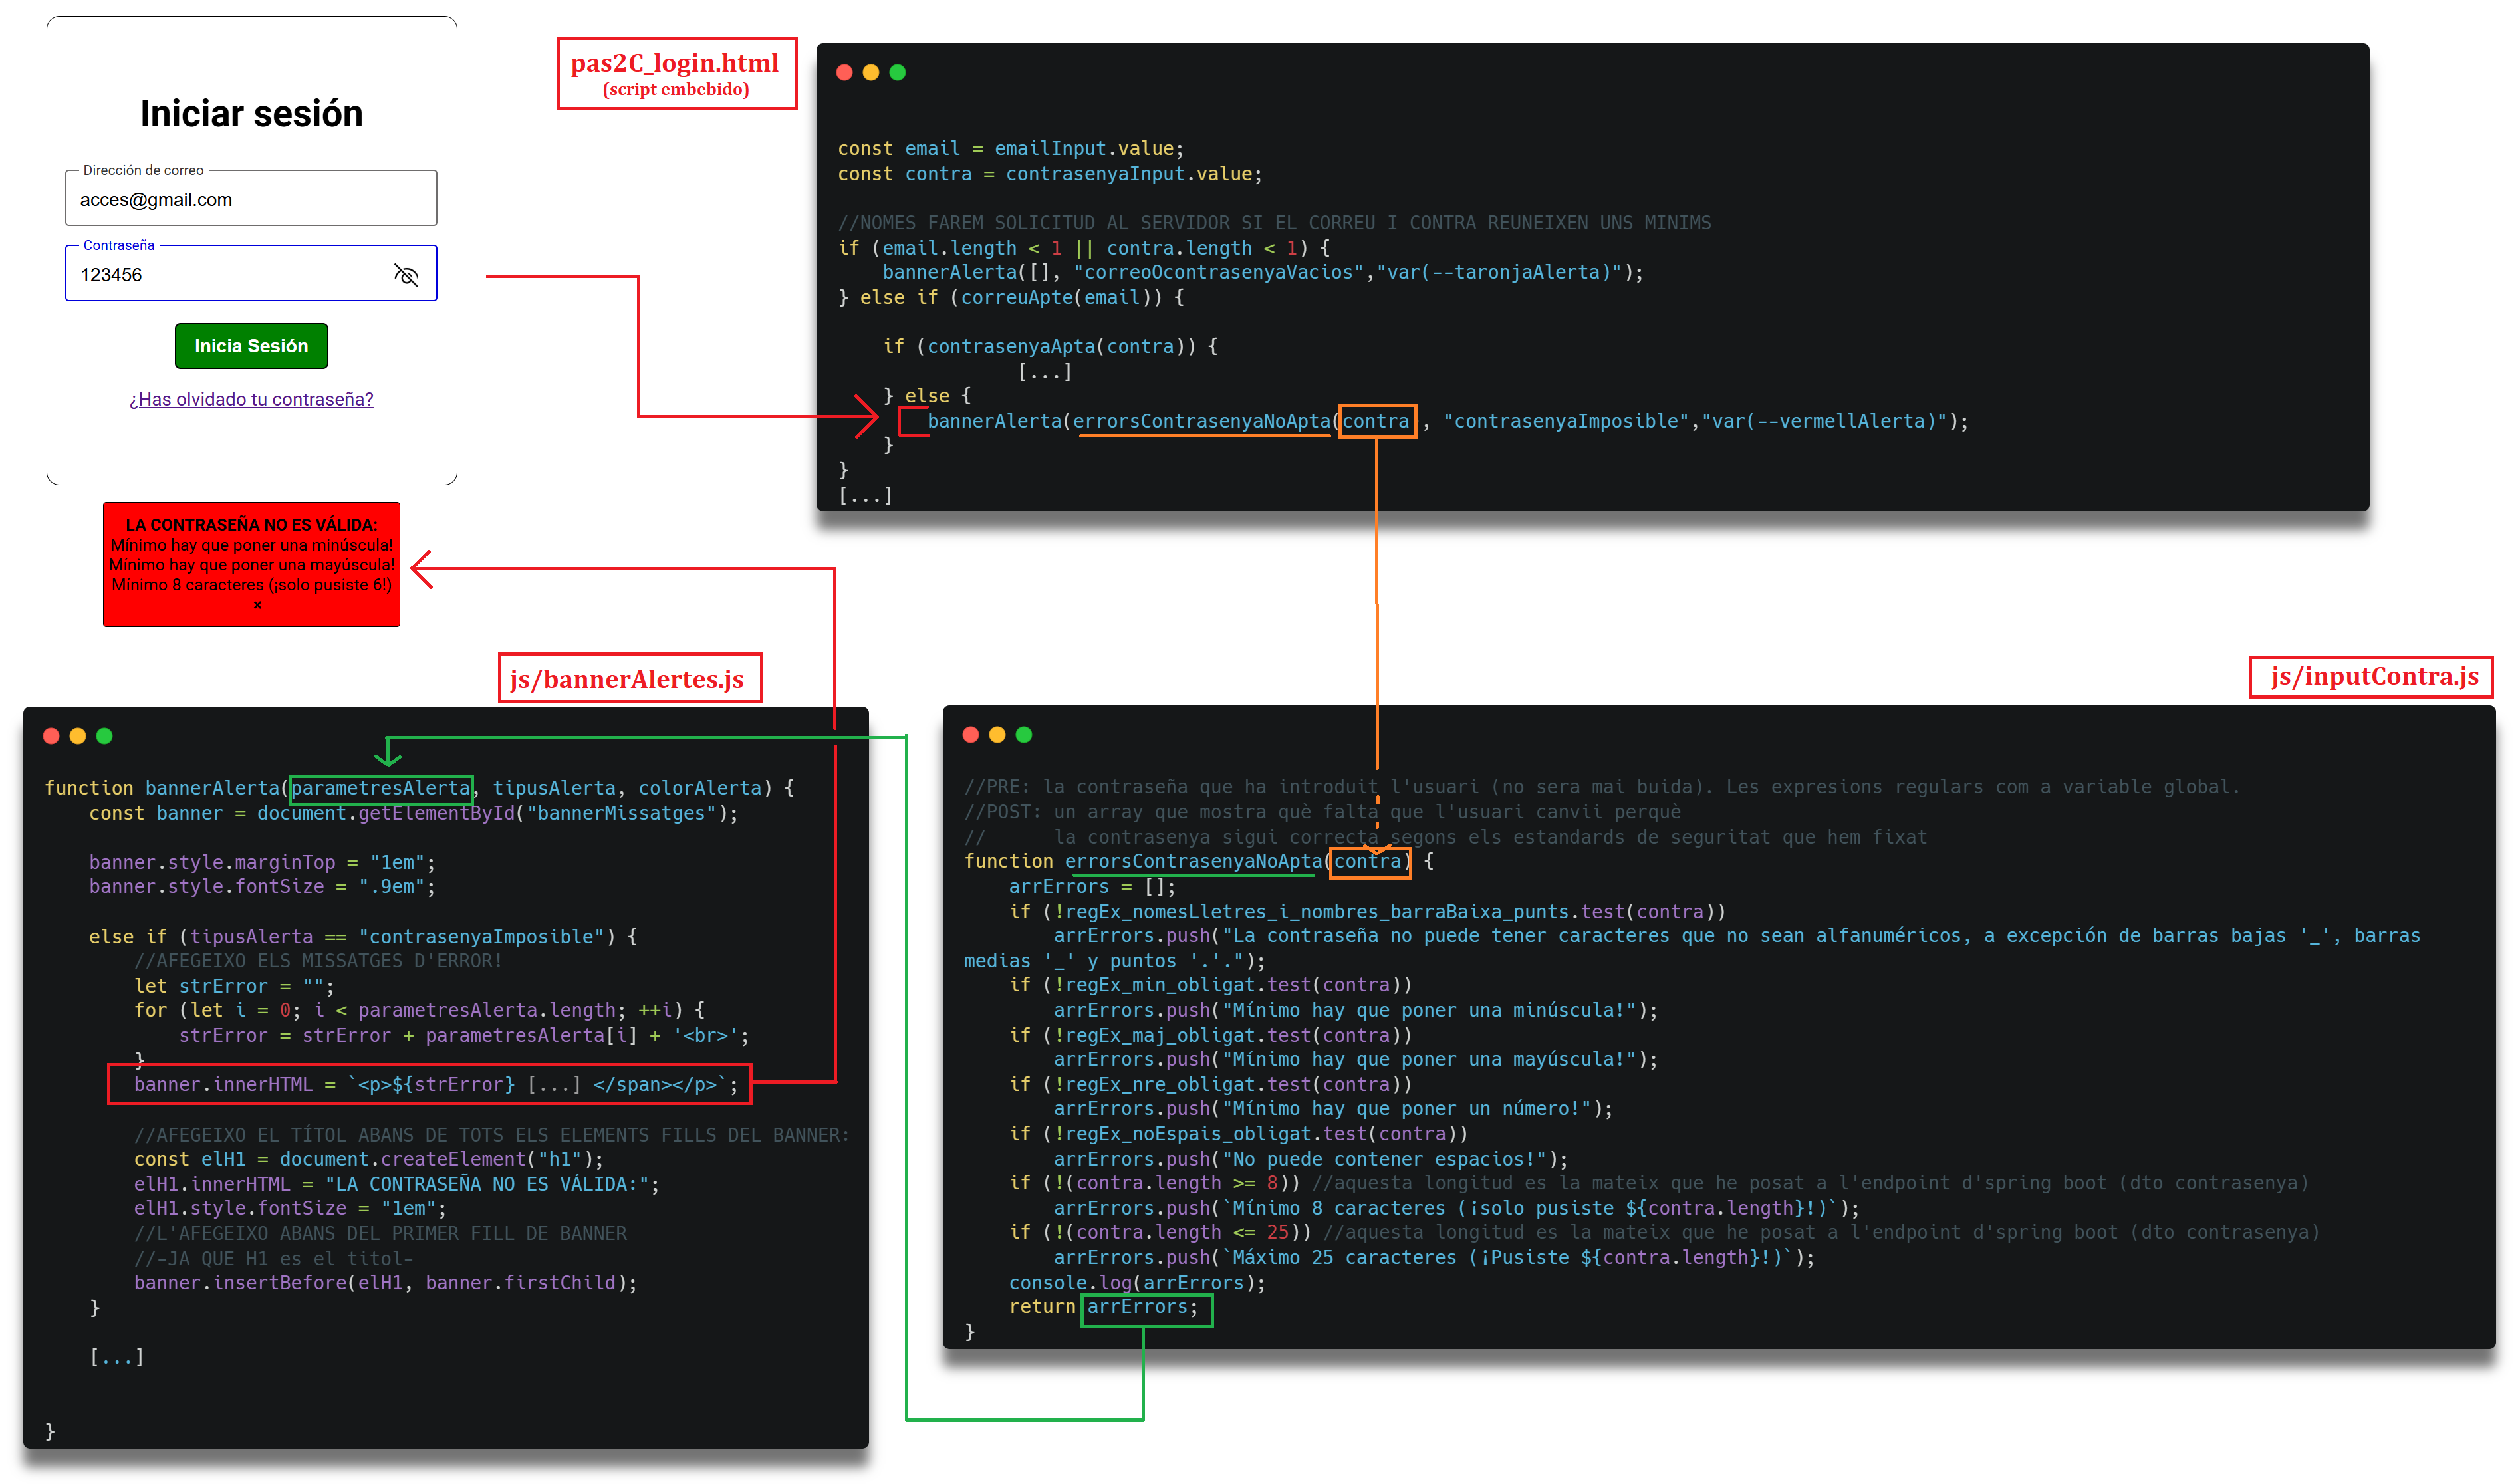
\includegraphics[width=1\linewidth]{img/activacioBannerAlertesLoginContrasenya}
			\label{fig:activacioBannerAlertesLoginContrasenya}
		\end{figure}
		\FloatBarrier
		
		
		
		
		
		
		
		
	
	\subsection{Diseño (UX/UI): páginas publicas}
	\label{sec:disenyoPublicas}
	
	El diseño de las páginas públicas (es decir, los archivos html que no son ni el dashboard ni el pas4\_) también son responsive. Tienen por ahora un diseño minimalista para no distraer al usuario y facilitarle su registro. A continuación se puede ver como las distintas media queries afectan a dos de las páginas públicas:
	
	\FloatBarrier
	\setlength{\belowcaptionskip}{3pt}
	\begin{figure}[H]
		\centering
		\caption{Arriba vemos la parte superior de index.html. Debajo la página de inicio de sesión. De izquierda a derecha: vista de escritorio, tablet y móvil gracias a media queries en el CSS.}
		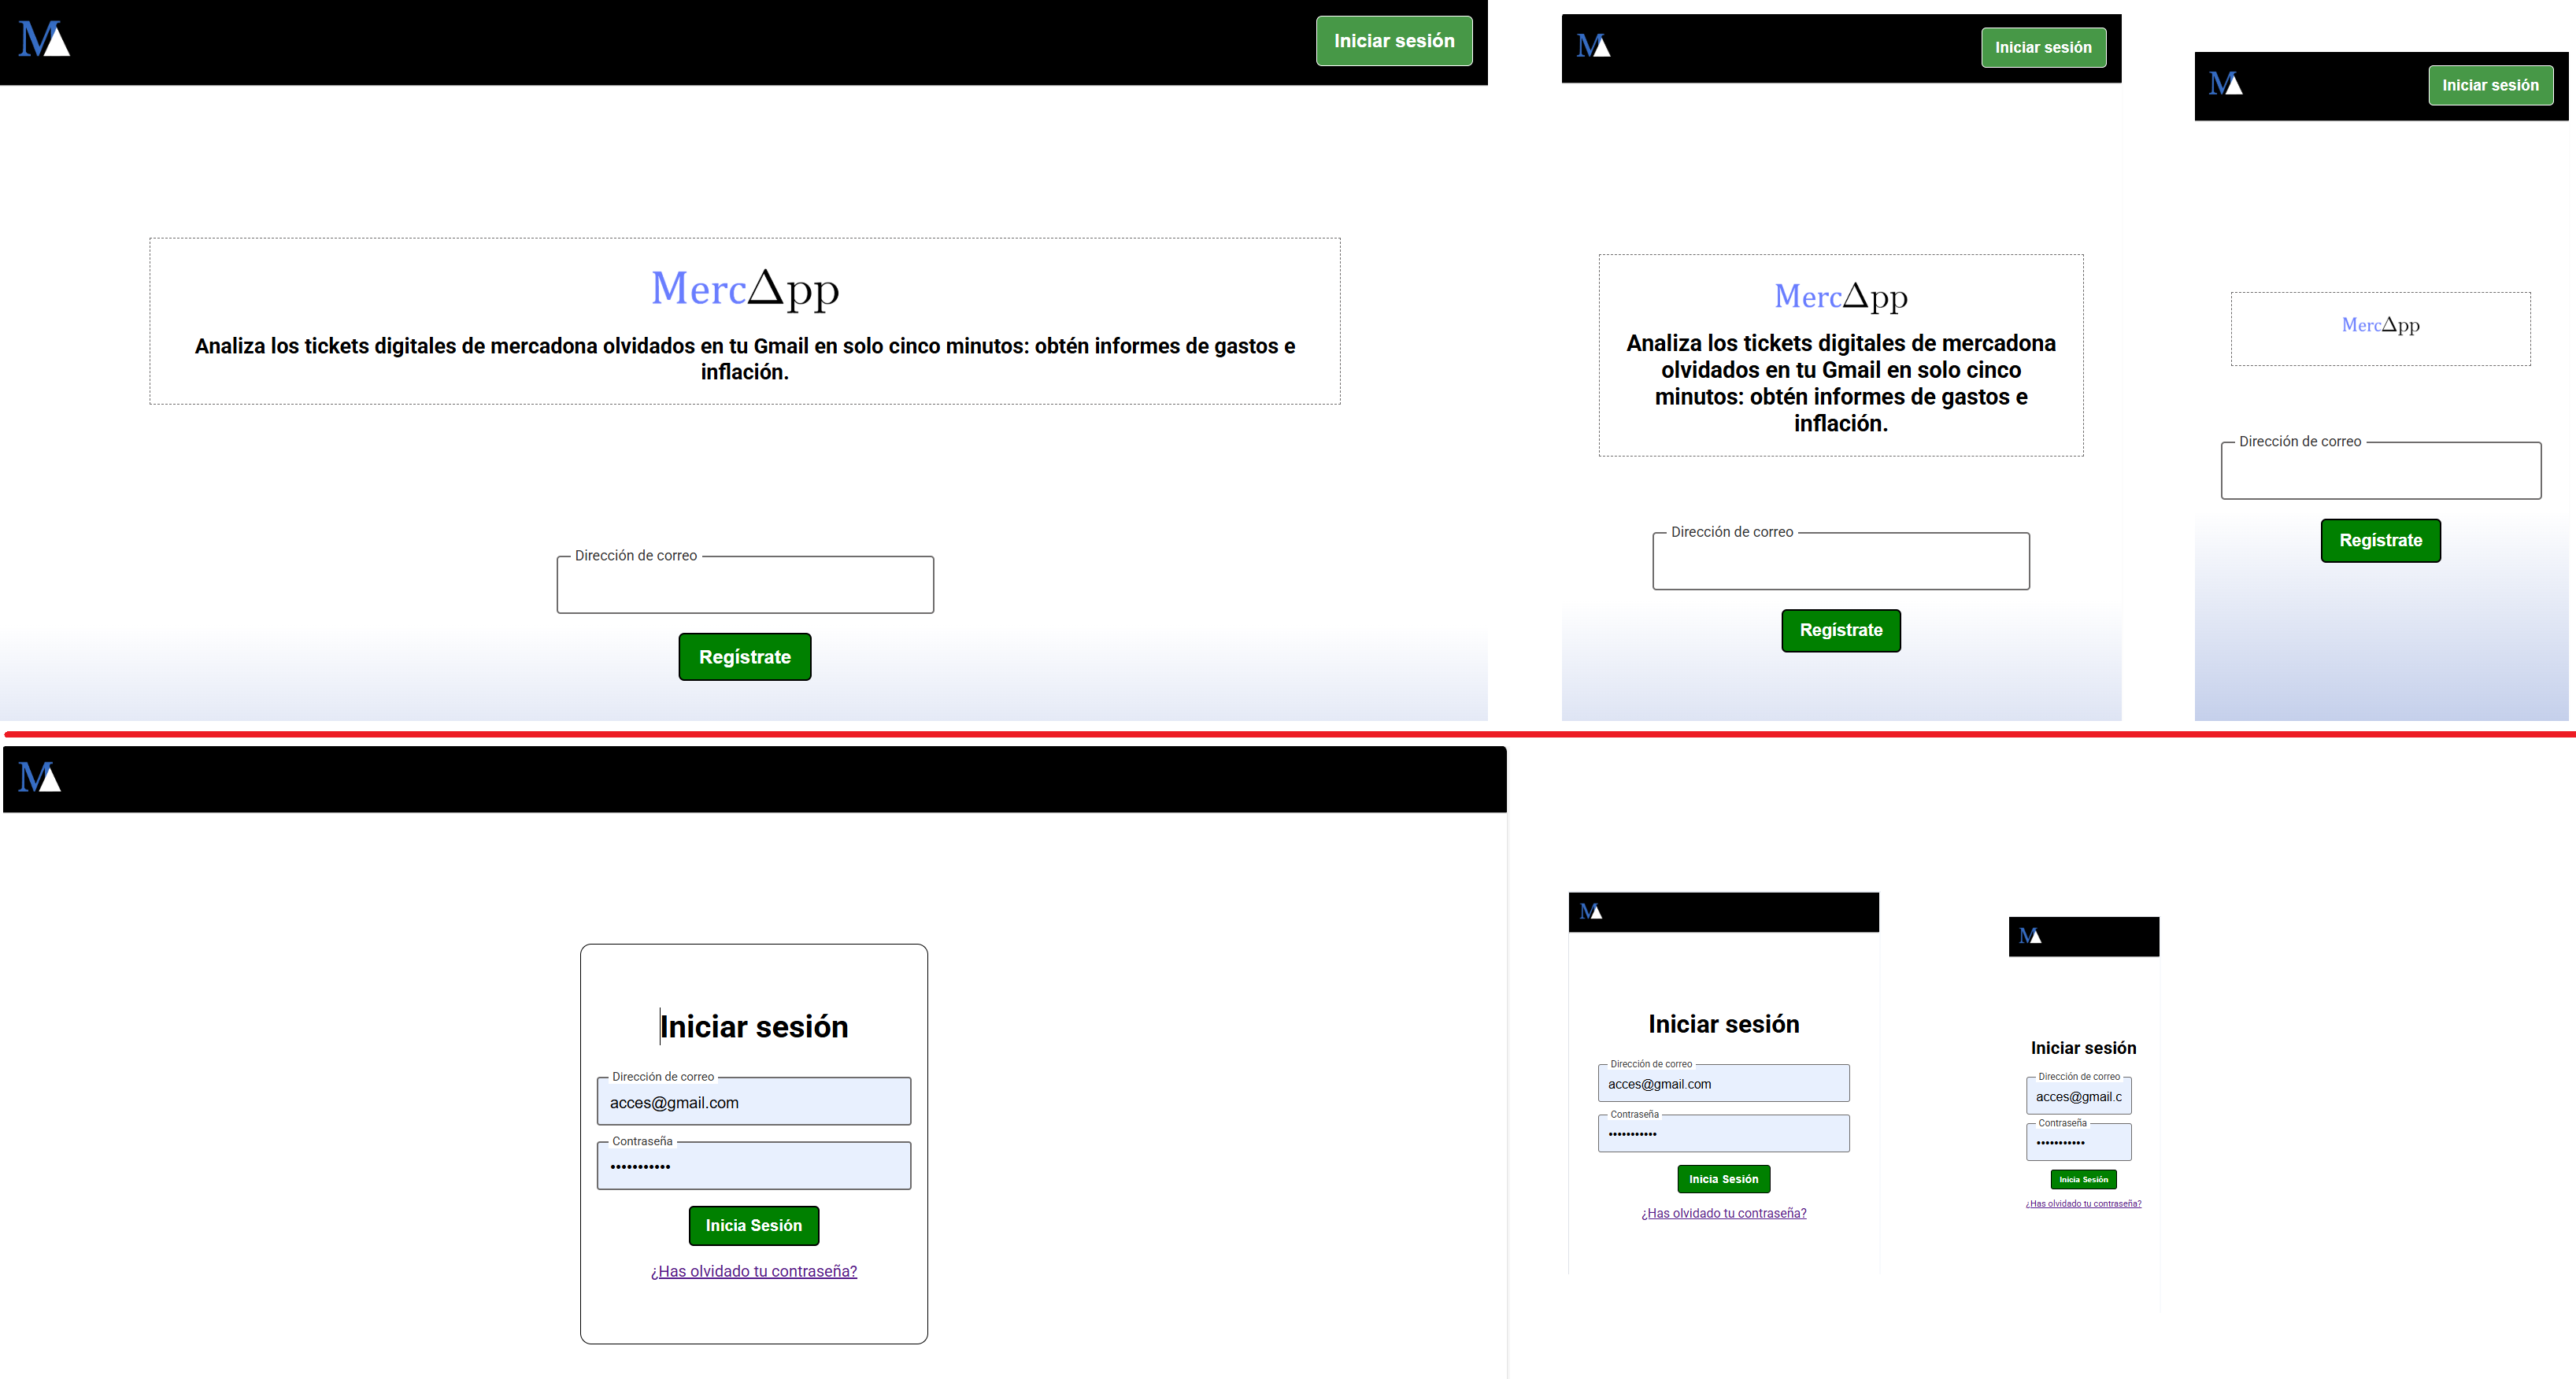
\includegraphics[width=1\linewidth]{img/mediaQueryIndexhtml}
		\label{fig:mediaQueryIndexhtml}
	\end{figure}
	\FloatBarrier
	
	Las media queries de las páginas públicas se han separado en distintos archivos. Por ejemplo, la barra de navegación de \texttt{index.html}, \texttt{pas2A\_infoBenvinguda}, \texttt{pas2B\_introduirContrasenya} y \texttt{pas2C\_login} tienen sus estilos y su media query aplicadas todos en el archivo siguiente: \href{https://github.com/blackcub3s/mercApp/blob/main/APP%20WEB/__frontend__produccio__/app/css/barraNavegacioSimple.css}{css/barraNavegacioSimple.css}. Dado que no hemos utilizado un framework de javascript que nos permita desarrollar en componentes hemos visto pertinente tratar de modularizar en la medida de lo posible aquello que hemos desarrollado. Con lo cual todas estas páginas con una navbar incluyen este archivo en el \textit{head}.
	
	Nótese que los formularios para introducir correo y contraseña tiene el mismo aspecto tanto en \texttt{index.html} como en \texttt{pas2C\_login.html} y el botón de registro e inicio de sesión también son iguales. También hemos modularizado su CSS introduciéndolo en un mismo archivo, en la ruta: \href{https://github.com/blackcub3s/mercApp/blob/main/APP%20WEB/__frontend__produccio__/app/css/landing/inputText.css}{css/landing/inputText.css}
	
	Finalmente tenemos la footer del \texttt{index.html}: solo la hemos introducido por ahora en \texttt{pas4\_concedirAccesGmail.hml}(una de las páginas privadas), pero no en todas las demás páginas públicas: en algunas de estas últimas queremos solamente que los usuarios pongan contraseña o correo y no queremos distraer con detalles superfluos. De ahí que la barra de navegación de páginas públicas no tenga links en la navbar. Los links los encontramos una vez el usuario se registra. Sin embargo, a futuro se podría expandir la página del index.html para incluir una barra de navegación ligera con información de quienes somos y una footer en todas las páginas públicas.
	
	
	\FloatBarrier
	\setlength{\belowcaptionskip}{3pt}
	\begin{figure}[H]
		\centering
		\caption{Creación de la footer en \texttt{index.html} y en \texttt{pas4\_concedirAccesGmail.hml} con diseño minimalista: link a linkedin y \textit{display: flex} para centrar verticalmente y horizontalmente el mensaje en el espacio ocupado por la \textit{footer}}
		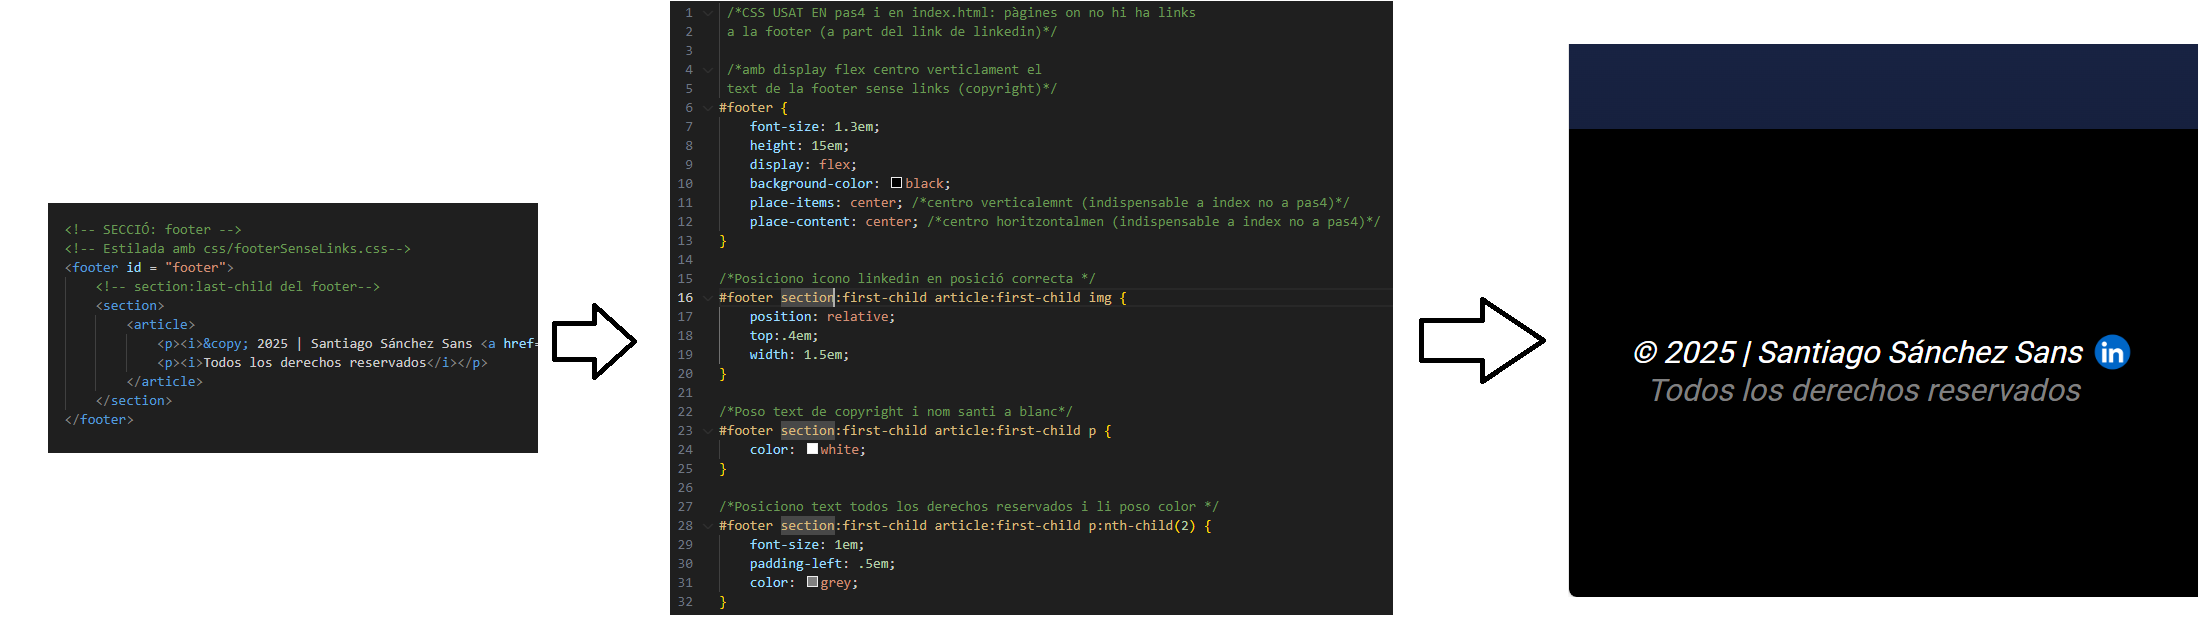
\includegraphics[width=1\linewidth]{img/footerIndexIpas4}
		\label{fig:footerIndexIpas4}
	\end{figure}
	\FloatBarrier
	
	
	
	
	
	
	\subsection{Diseño (UX/UI): páginas privadas}
	\label{sec:disenyoResponsivePrivadas}
	
	\subsubsection{Diseño del dashboard}
	
	Parte del diseño del dashboard es un reaprovechamiento del figma y del código HTML y CSS creado para el proyecto final de la asignatura de desarrollo de interfaces, concretamente, de una página donde se explicaban diferencias entre frameworks de front-end que el lector puede consultar  	\href{https://blackcub3s.github.io/proyectoDesarrolloInterfaces/FrontEnd.html}{aquí} para ver la semilla del diseño original.
	
	Esa página fue diseñada y programada por mí de forma íntegra, desde cero con CSS y HTML (a excepción de la Footer que la hizo mi compañero de grupo, dado que era un proyecto grupal). De la parte del footer no se ha aprovechado HTML ni CSS porque el código de la misma no fue de mi autoría, así que se ha optado por un diseño distinto.
	
	El motivo del reaprovechamiento del código es que era imposible asegurar una firma visual distintiva y un aspecto profesional con un diseño desde cero en el poco tiempo para hacer el proyecto. Para hacer la página original, fueron dedicadas muchas, \textit{muchísimas} horas por mi parte: una barbaridad de hecho, así que me sabía mal no reutilizarlo. Además, lo bueno de la reutilización es que se ha podido mejorar la página inicial con dos aspectos que en la asignatura de interfaces NO se pudieron cubrir por los requisitos de la misma:
	
	\vspace{-.8em}
	\begin{itemize}
		\setlength{\itemsep}{-.2em}
		\item \textbf{Diseño responsive}: la página original \texttt{frontEnd.html} del proyecto de interfaces no podía ser responsive mientras que \texttt{dashboard} sí lo es\footnote{en la medida de lo posible, dado que no todas las librerías admiten responsividad: por ejemplo, chart.js no lo es.}.
		\item \textbf{Persistencia de datos}: las vistas de la página del dashboard permiten visualizar datos extraídos de una base de datos de mongoDB.
	\end{itemize}
	
	\noindent Después de esta aclaración vamos a pasar a explicar las secciones del \texttt{dashboard} y de su diseño.
	
	
	
	\noindent \textbf{SECCIÓN 0 (S0): barra de navegación y botón de cierre de sesión}
	\hrule
	\vspace{.5em}
	
	Esta sección incorpora el botón de cierre de sesión (que elimina el token de acceso, en realidad, como ya se ha visto en la sección \ref{sec:tancarSessioBotoExplicacio}) y la barra de navegación que conseguirá redirigir a ubicaciones distintas en función de si se es usuario (permisos=1) o superusuario (permisos=2). También muestra links a páginas que nos permiten ver los tickets del usuario (si los tiene descargados), sus datos en una tabla y una página para contactar con nosotros (ver figuras \ref{fig:barranavegaciodashboardpermisos1}, \ref{fig:barranavegaciodashboardpermisos1dropdown} y \ref{fig:detalleNavbarDesplegadaCodi}).
	
	Además se ha utilizado un sistema (figura \ref{fig:linkAhover})para conseguir que al hacer hover en cada link cambie su color a gris y aparezca una línea por debajo con una transición suave (automatizando las propiedades\textit{border-bottom} y \textit{color}) . Se ha tenido especial cuidado en que el añadir la línea debajo NO desplace el resto de la página hacia abajo. Para evitarlo todos los links tienen en realidad una línea por debajo del mismo color del fondo, que solo cambia de color al pasar por encima. Hay muchas líneas de código para conseguirlo y redirigimos al lector al github para verlas (nótese el uso de selectores descendientes, por norma: \href{https://github.com/blackcub3s/mercApp/blob/main/APP%20WEB/__frontend__produccio__/app/css/dashboard/navFooter.css}{link a navFooter.css})
	
	\FloatBarrier
	\setlength{\abovecaptionskip}{3pt}
	\begin{figure}[H]
		\centering
		\caption{Barra de navegación del usuario de permisos=1 con sus 4 elementos}
		
\includegraphics[width=1\linewidth]{img/barraNavegacioDashboardPERMISOS1}

		\label{fig:barranavegaciodashboardpermisos1}
	\end{figure}
	\FloatBarrier
	
	Dentro de la sección servicios hay un desplegable o ``dropdown" que nos permite llegar a las distintas secciones del dashboard: el ``inflalyzer'', el ``categorizer'' y el ``intervalizer''.
	
	\FloatBarrier
	\setlength{\belowcaptionskip}{3pt}
	\begin{figure}[H]
		\centering
		\caption{Detalle barra de navegación con el drop-down desplegado.}
		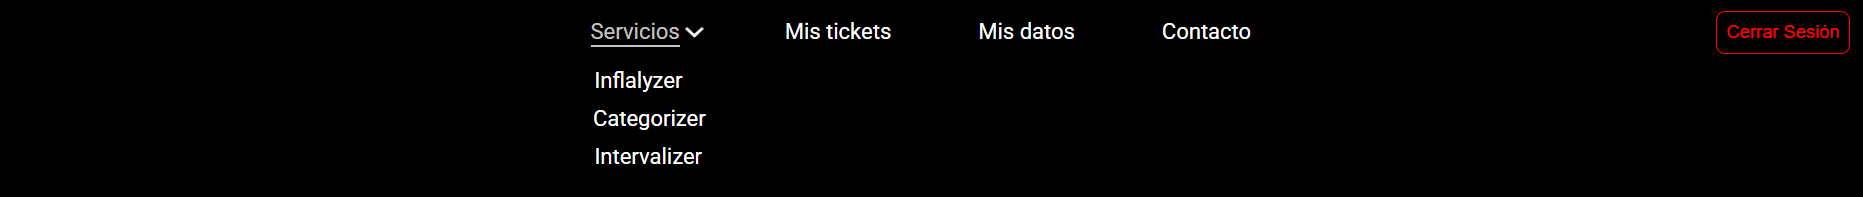
\includegraphics[width=1\linewidth]{img/barraNavegacioDashboardPERMISOS1dropDown}
		
		\label{fig:barranavegaciodashboardpermisos1dropdown}
	\end{figure}
	\FloatBarrier
	
	
	\FloatBarrier
	\setlength{\belowcaptionskip}{0pt}
	\begin{figure}[H]
		\centering
		\caption{Detalle del código que hizo posible el drop-down del menú. Cada elemento drop down se ha animado mediante animate.css definiendo distintas duraciones de la animación \textit{fadeInDown} para conseguir un efecto persiana. El uso del selector descendiente y el no abuso de los IDs a menos que sea necesario es una metodología seguida a lo largo del diseño del dashboard.}
		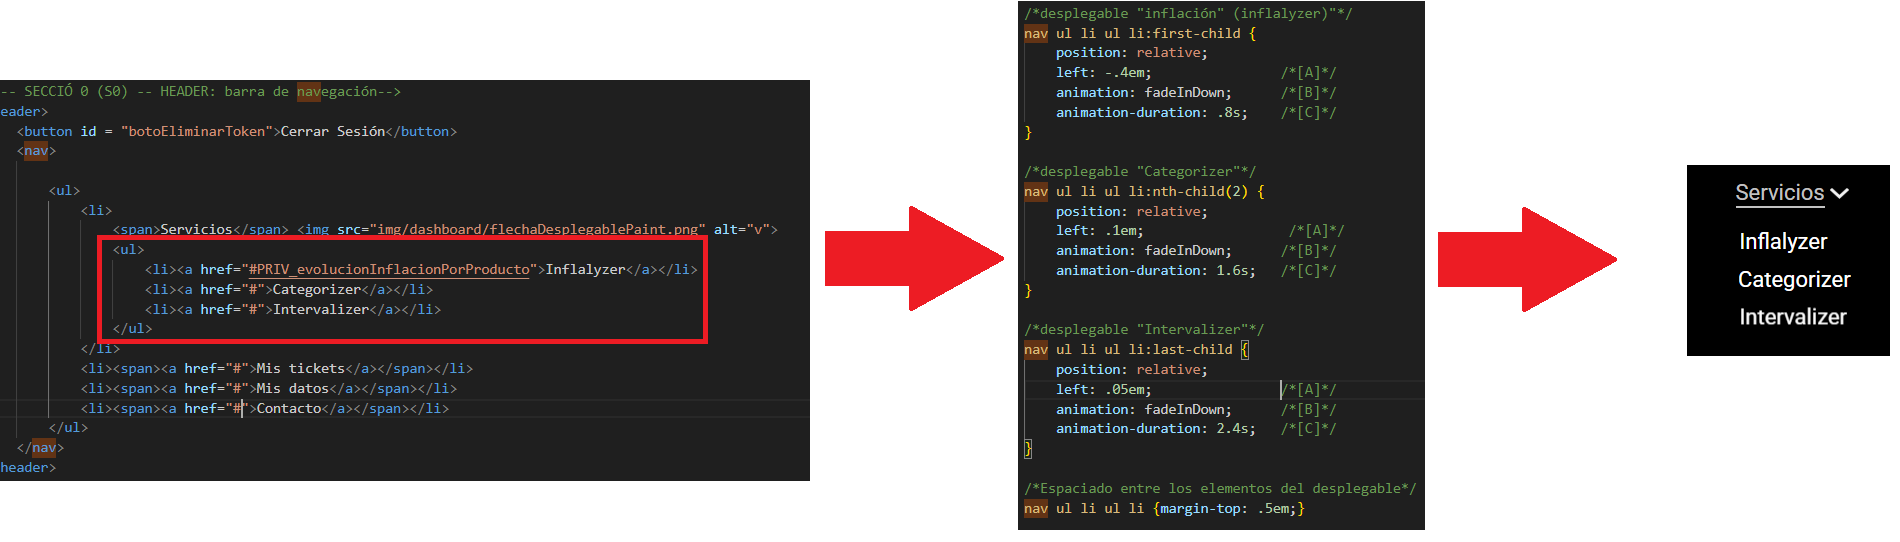
\includegraphics[width=1\linewidth]{img/navBarDesplegadaMakingOfPermisos1.png}

		\label{fig:detalleNavbarDesplegadaCodi}
	\end{figure}
	\FloatBarrier
	
	\FloatBarrier
	\begin{figure}[H]
		\centering
		\caption{Transiciones suaves de propiedades \textit{border-bottom }y \textit{color} al hacer hover en los spans que envuelven los links tanto en la barra de navegación como en la footer.}
		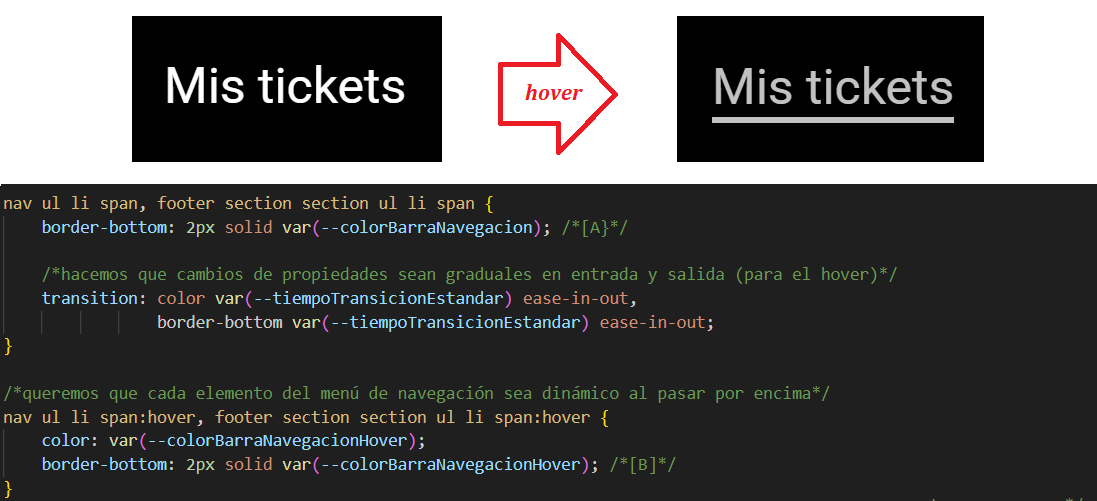
\includegraphics[width=1\linewidth]{img/linkAhover.png}
		
		\label{fig:linkAhover}
	\end{figure}
	\FloatBarrier
	
	
	
	
	
	
	
	
	\noindent \textbf{SECCIÓN 1 (S1): presentación Dashboard}
	\hrule
	\vspace{.5em}
	
	Esta sección simplemente muestra un gradiente lineal que transiciona del negro de la barra de navegación hacia el azul claro que es colindante a la barra roja. Para hacerlo se ha hecho mediante un doble gradiente lineal. También se ha usado la clase fadeIn de animate.css para hacer que aparezca con un fundido de entrada al cargar o recargar la página. Podéis ver la figura que muestra el código en \ref{fig:S1FrontMakeOf}.
	
	\FloatBarrier
	\setlength{\belowcaptionskip}{3pt}
	\begin{figure}[H]
		\centering
		\caption{De izquierda a derecha: código HTML, codigo CSS y el resultado final de la vista de esa sección}
		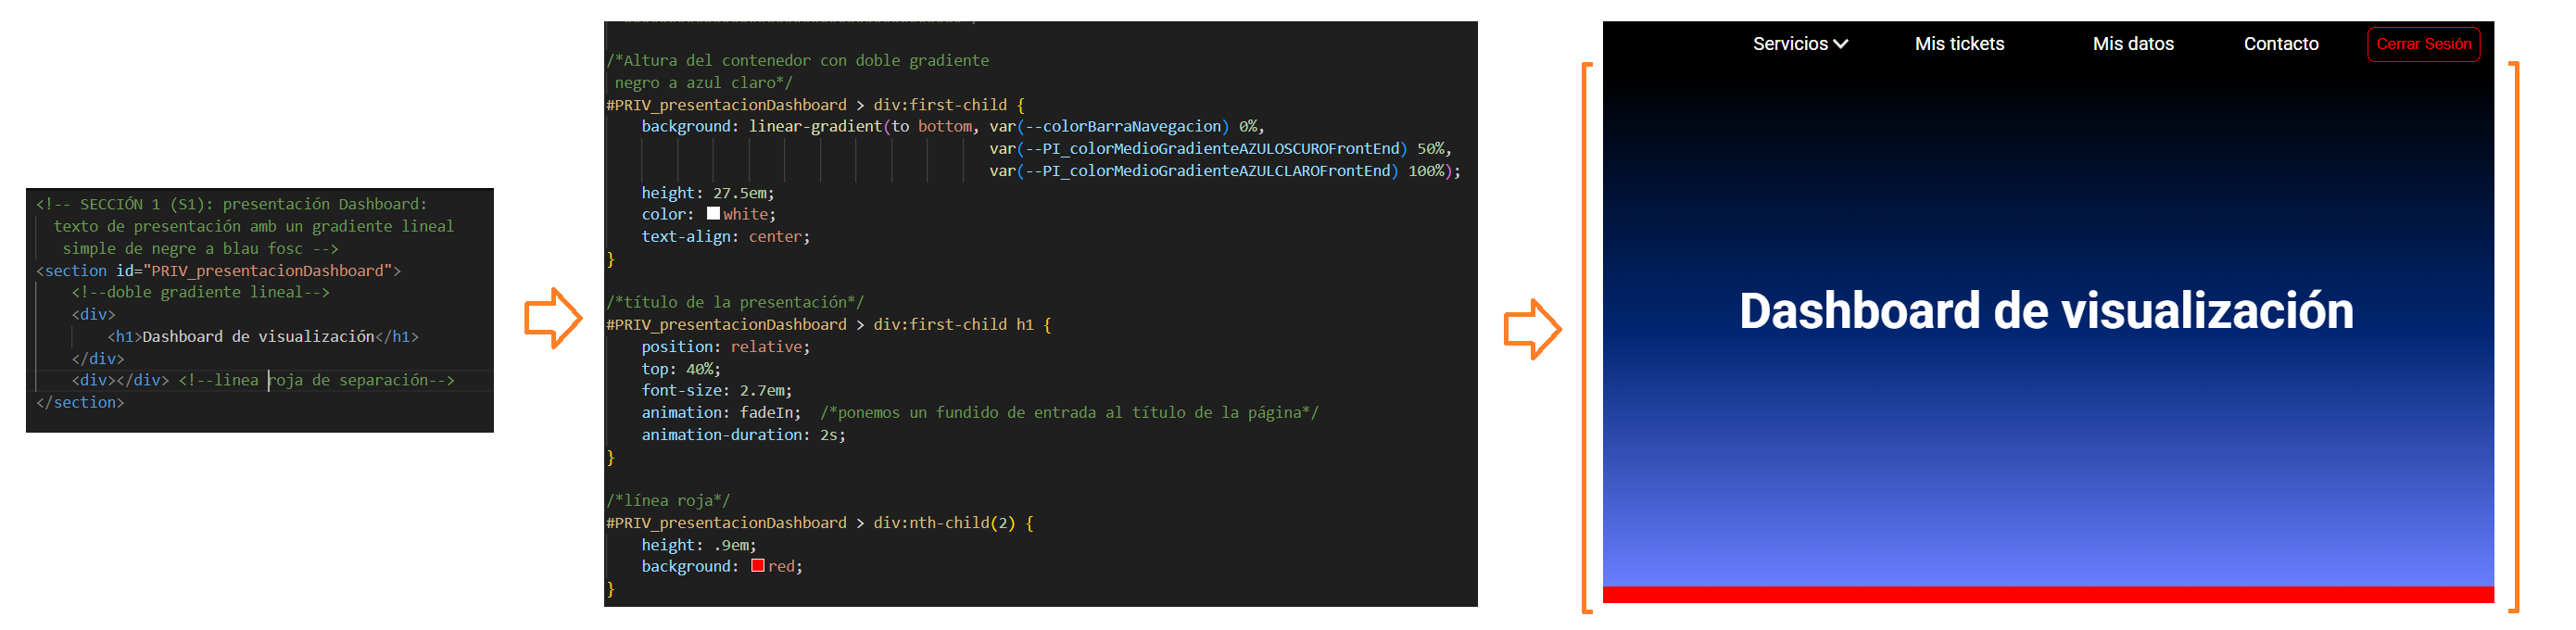
\includegraphics[width=1\linewidth]{img/S1FrontMakeOf.png}
		
		
		\label{fig:S1FrontMakeOf}
	\end{figure}
	\FloatBarrier
	
	
	
	
	\noindent \textbf{SECCIÓN 2 (S2): características de la aplicación mercApp:}
	\hrule
	\vspace{.5em}
	
	Esta sección contiene tres ``cards'' que resumen los servicios que ofrece el resto del dashboard (inflación por producto, gastos por categoría y gastos por ventana temporal): también incorporan los datos más relevantes de los tikets de cada usuario, que se extraen también de la BBDD (ver detalle figura \ref{fig:s2caracteristiquesmercapp}). El lector puede consultar el fichero \href{https://github.com/blackcub3s/mercApp/blob/main/APP%20WEB/__frontend__produccio__/app/css/dashboard/estils.css}{estils.css} todos los selectores css descendientes que empiezan por el id con el que encabezamos el section de esa parte (id \textit{PRIV\_caracteristicasDashboard}).

	
	De estas cards hay tres aspectos a destacar: En \textit{primer lugar}, se ha vigilado en que sigan exactamente la proporción áurea. Al crearlas se ha definido la propiedad CSS \textit{aspect-ratio} (\href{https://github.com/blackcub3s/mercApp/blob/663360ea63eafd38c1fa052e7a994e22d7f0a5f6/APP%20WEB/__frontend__produccio__/app/css/dashboard/estils.css#L80}{ver en GitHub} para que la relación de aspecto ancho-alto de cada una de ellas sea exactamente de 1 a 1.618 \cite{wikiPropAurea}. De este modo, creamos un rectángulo agradable a la vista para poder presentar los primeros datos del resumen de los tickets al usuario. \textit{En segundo lugar}, en cada una de las cards se ha usado un gradiente lineal vertical mediante la propiedad CSS \textit{background} (\href{https://github.com/blackcub3s/mercApp/blob/663360ea63eafd38c1fa052e7a994e22d7f0a5f6/APP%20WEB/__frontend__produccio__/app/css/dashboard/estils.css#L85}{ver línea}) que hemos utilizado también para cambiar dinámicamente ambos colores del gradiente al hacer hover (\href{https://github.com/blackcub3s/mercApp/blob/663360ea63eafd38c1fa052e7a994e22d7f0a5f6/APP%20WEB/__frontend__produccio__/app/css/dashboard/estils.css#L126}{ver línea}). En esos casos, además el hover altera también el \textit{box-shadow} definido en esta \href{https://github.com/blackcub3s/mercApp/blob/663360ea63eafd38c1fa052e7a994e22d7f0a5f6/APP%20WEB/__frontend__produccio__/app/css/dashboard/estils.css#L84}{línea} y lo modifica a otro valor (\href{https://github.com/blackcub3s/mercApp/blob/663360ea63eafd38c1fa052e7a994e22d7f0a5f6/APP%20WEB/__frontend__produccio__/app/css/dashboard/estils.css#L125}{en esta}). El resultado de esta programación es el que se puede ver en la figura \ref{fig:cardCaracteristicaAbansDespres}. También se han definido automatizaciones de la propiedad \textit{transform} para las imágenes de dentro de las cards, para hacer que aumenten de tamaño al posarnos con el ratón por encima (\href{https://github.com/blackcub3s/mercApp/blob/663360ea63eafd38c1fa052e7a994e22d7f0a5f6/APP%20WEB/__frontend__produccio__/app/css/dashboard/estils.css#L106-L108}{detalle líneas}).
	
	Finalmente, merece la pena mencionar que mediante wow.js se ha conseguido crear las animaciones de animate.css (como las que se usaron en la sección 0, ver captura previa \ref{fig:detalleNavbarDesplegadaCodi}) de modo que en lugar de que aparezcan con un temporizador desde la carga de la página como nos permite la librería animate.css, sino que aparezcan con un temporizador desde que hacemos scroll a la sección que las incluye.
	
	Así las cosas, las propiedades que nos define animate.css en este caso no las hemos escrito en el CSS sino que lo hemos hecho en el propio HTML de acuerdo con el requerimiento de la librería \textit{wow.js}. De este modo al hacer scroll a la sección, la card de la izquierda aparecerá por la izquierda (fadeInLeft,  \href{https://github.com/blackcub3s/mercApp/blob/663360ea63eafd38c1fa052e7a994e22d7f0a5f6/APP%20WEB/__frontend__produccio__/app/dashboard.html#L130}{link}), la del medido de abajo (fadeInUp,  \href{https://github.com/blackcub3s/mercApp/blob/663360ea63eafd38c1fa052e7a994e22d7f0a5f6/APP%20WEB/__frontend__produccio__/app/dashboard.html#L153}{link}) y la de la derecha de esa misma dirección (fadeInRight,  \href{https://github.com/blackcub3s/mercApp/blob/663360ea63eafd38c1fa052e7a994e22d7f0a5f6/APP%20WEB/__frontend__produccio__/app/dashboard.html#L173}{link}). Una ves hecho esto se ajustó la duración y el \textit{delay} de cada propiedad mediante atributos en esas mismas líneas del HTML.
	
	
	\FloatBarrier
	\begin{figure}[H]
		\centering
		\caption{Detalle de la sección con las tres cards: características resumidas del dashboard. Los textos en color son placeholders para lo que se extraerá de la BBDD.}
		\label{fig:s2caracteristiquesmercapp}
		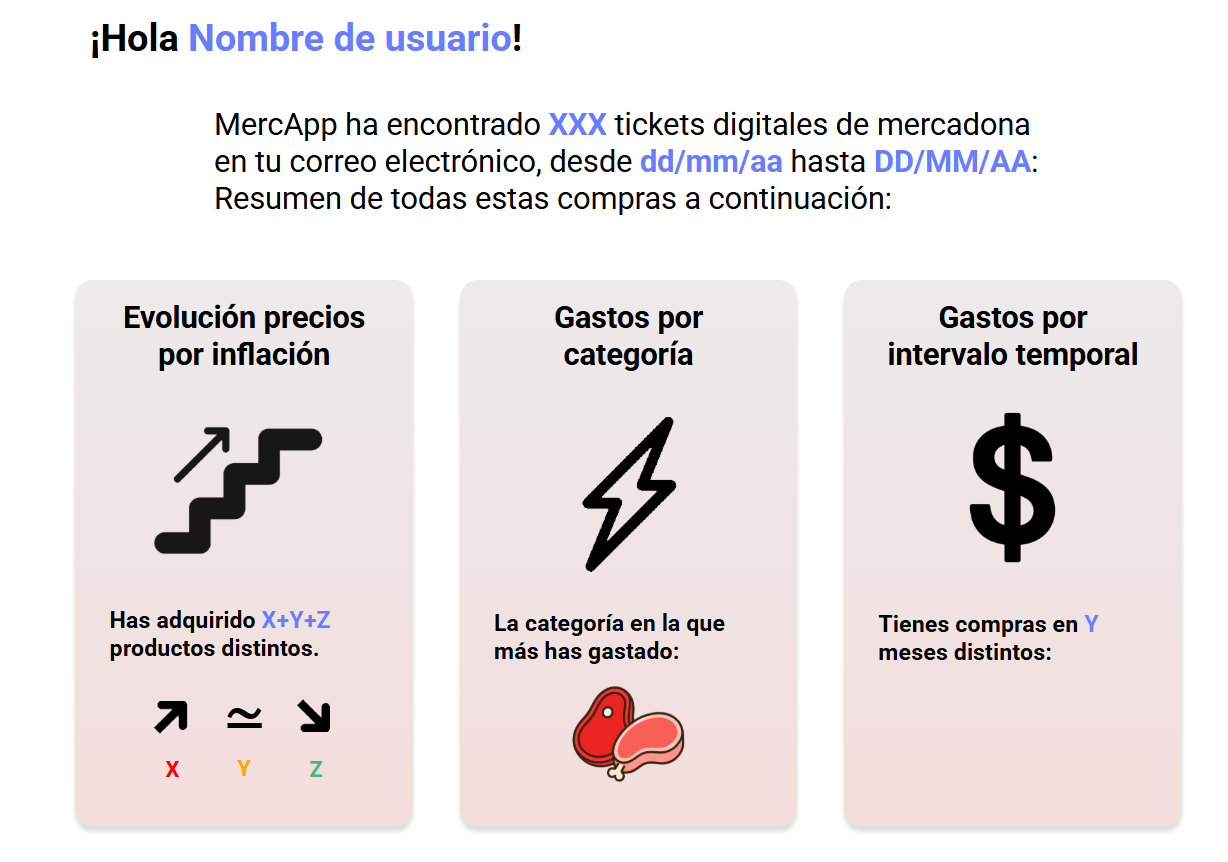
\includegraphics[width=1\linewidth]{img/s2CaracteristiquesMercApp.png}
	\end{figure}
	\FloatBarrier
	
		\FloatBarrier
	\begin{figure}[H]
		\centering
		\caption{Detalle del impacto que tiene la automatización de \textit{box-shadow} y \textit{background} al hacer hover encima de las cards.}
		\label{fig:cardCaracteristicaAbansDespres}
		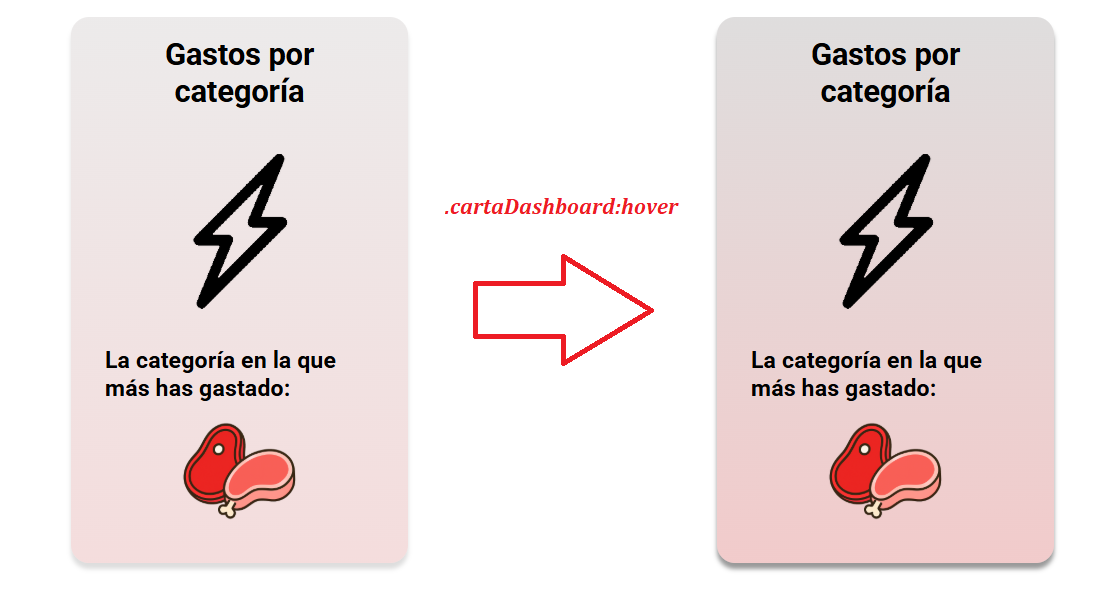
\includegraphics[width=1\linewidth]{img/cardCaracteristicaAbansDespres.png}
	\end{figure}
	\FloatBarrier
	
	
	
	\noindent \textbf{SECCIÓN 3 (S3): ``inflalyzer'' (sin swiper: ¡esta vez hecho a mano!) }
	\hrule
	\vspace{.5em}
	En la página original de la que hemos derivado parte del dashboard (\href{https://blackcub3s.github.io/proyectoDesarrolloInterfaces/FrontEnd.html}{link}) utilizamos la librería swiper para cambiar entre imágenes de una galería mediante clicks en unos paginadores (si no podéis ver la web, podéis ver detalle en figura \ref{fig:swiperFront} del anexo). Tratar de reutilizarlo para nuestro caso fue imposible: ahora no tenemos solo imágenes a ir variando con los paginadores, sino que tenemos una tabla entera a poner dentro de esos paginadores. Swiper esto no lo podía manejar.
	
	Así las cosas hubo que crear un swiper manualmente para poder albergar una tabla dentro del paginador (ver figura \ref{fig:imatgeSwiperCustom}). Este ``swiper'' artesanal, se creó tomando los mismos iconos de swiper, eliminado el canal alpha del fondo, cambiando su color de azul a rojo y definiendo eventos de click a las imágenes que conforman esas flechitas.
	
	\FloatBarrier
	\begin{figure}[H]
		\centering
		\caption{Detalle de la parte superior del intervalizer: obsérvese el paginador creado manualmente}
		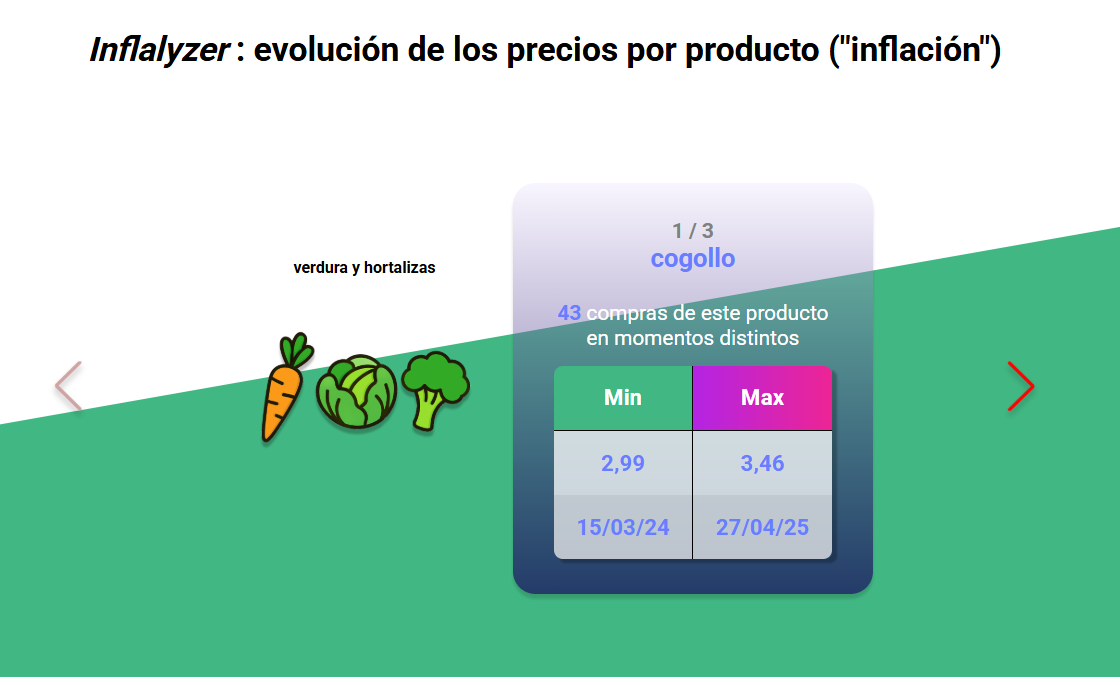
\includegraphics[width=1\linewidth]{img/imatgeSwiperCustom.png}
		\label{fig:imatgeSwiperCustom}
	\end{figure}
	\FloatBarrier
	
	A nivel de UX/UI el paginador de la figura \ref{fig:imatgeSwiperCustom} ha seguido los mismos principios. En este caso, hay un par de cosas destacables. El uso de imágenes customizadas para los botones de paginación nos ha habilitado para usar \textit{hover} afectando la propiedad \textit{drop-shadow} de la imagen del paginador, para así aprovechar los contornos del mismo hacer transform y dar la sensación de profundidad \textbf{combinando la sombra con el incremento de tamaño} (ver imagen \ref{fig:paginadorscustom}).
	

	\FloatBarrier
	\begin{figure}[H]
		\centering
		\caption{Paginadores para moverse hacia productos con más frecuencia de compra: a la izquierda sin hover (drop-shadow difuso y poco visible) y con hover a la derecha de la captura (drop-shadow con menos difusión de imagen y ligeramente desplazado hacia abajo).}
		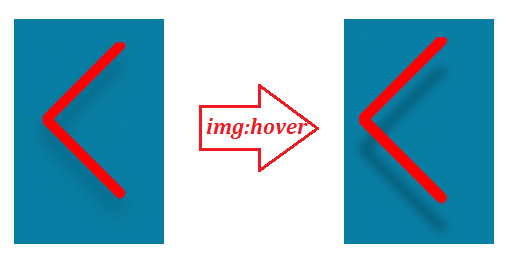
\includegraphics[width=1\linewidth]{img/paginadorsCustom}

		\label{fig:paginadorscustom}
	\end{figure}
	\FloatBarrier
	
	Asimismo, cuando llegamos al final del listado de productos del usuario, sea por la izquierda o la derecha, se cargan unas imágenes difuminadas que además con JavaScript no permitimos que traten de acceder a ningún dato (\href{https://github.com/blackcub3s/mercApp/blob/main/APP%20WEB/__frontend__produccio__/app/img/dashboard/paginadorEsqDifuminat.png}{ver detalle}).
	
	El CSS de la imagen \ref{fig:imatgeSwiperCustom} está disponible en este rango de líneas de GitHub \href{https://github.com/blackcub3s/mercApp/blob/4ddc34194763af7a246ffabb14146ad9b4b2c5db/APP%20WEB/__frontend__produccio__/app/css/dashboard/estils.css#L155}{link}. Para observar el JavaScript de la paginación se puede visualizar el apartado \ref{sec:paginadorJavascriptArquitectura}.
	
	
	
	
	\noindent \textbf{SECCIÓN 4 (S4): ``categoryzer'' y SECCIÓN 5 (S5): ``intervalizer''}
	\hrule
	\vspace{.5em}
	
	Estas dos secciones todavía no tienen diseño y, por lo tanto, todavía no tienen CSS asociado. Cuando esté hecho el CSS aparecerá dentro del mismo archivo donde se han programado las tres secciones anteriores, con los debidos encabezados explicativos para distinguirlas de las demás: \href{https://github.com/blackcub3s/mercApp/blob/4ddc34194763af7a246ffabb14146ad9b4b2c5db/APP%20WEB/__frontend__produccio__/app/css/dashboard/estils.css}{/css/dashboard/estils.css}
	
	
	\subsubsection{Diseño del ``pas4\_concedirAccesGmail.html''}
	\label{sec:dissenyHtmlCSSpas4}
	
	El diseño del pas4 no entraña mucha más dificultad que el diseño del dashboard. Se ha seguido un procedimiento parecido para la generación de iconos que en el dashboard (los iconos generados se hicieron con IA y se extrajo el canal alpha con gimp más alguna edición extra en caso de ser necesaria: podéis verlos en la carpeta de \href{https://github.com/blackcub3s/mercApp/tree/main/creacioIconos/iconosPas4}{edición de iconos}).
	
	El icono para cerrar sesión es el mismo que en el dashboard y se han eliminado todos los links de la navBar. Luego se ha definido para la versión desktop un grid con dos columnas, alternando imágenes y texto, tal que así:
	
	\FloatBarrier
	\begin{figure}[H]
		\centering
		\caption{Vista del grid de dos columnas del \texttt{pas4\_concedirAccesGmail.html} en la versión desktop. En los círculos en rojo saldrán mensajes informativos que mostrarán mensajes al usuario sobre el número de tickets subidos (Paso 2, rojo) y el éxito o no de la extracción de datos (Paso 3, verde)}
		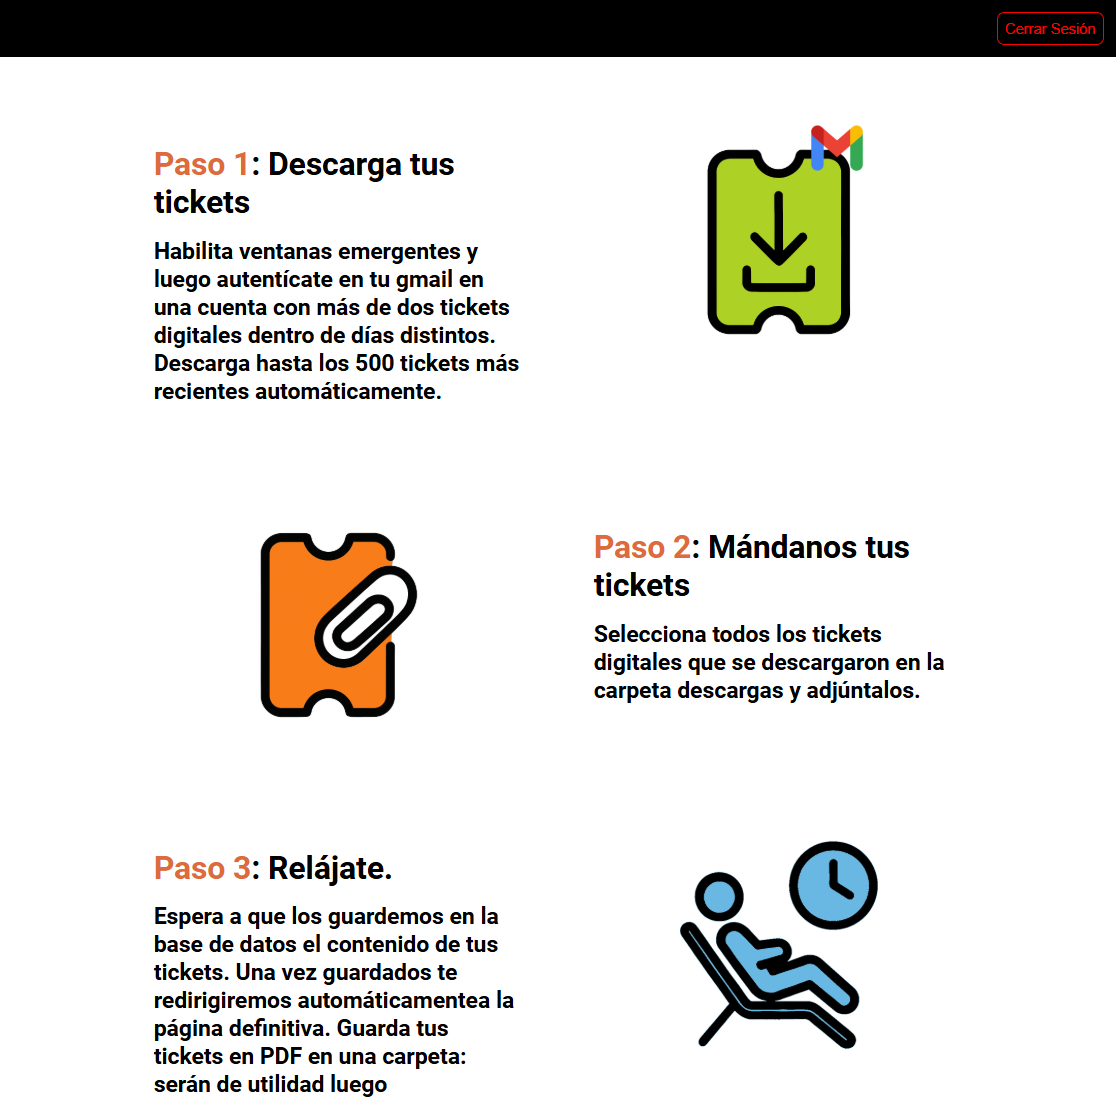
\includegraphics[width=.95\linewidth]{img/pas4Grid2cols}

		\label{fig:pas4grid2cols}
	\end{figure}
	\FloatBarrier
	
	Un aspecto diferencial con el \textbf{dashboard} es que el diseño responsive ha implicado generar una media query en la que le pedíamos en los selectores descendientes que invirtieran el orden en el que aparecían el contenedor de las imágenes en relación al contenedor del texto (h1 y h2): nótese que en el HTML el icono descarga de tickets y el icono del engranaje aparecen después del contenedor del texto porque queremos hacer que aparezcan a la derecha: así alternan los iconos y el texto en la vista de escritorio en un grid de dos columnas. 
	
	Sin embargo, este diseño de la versión de escritorio tiene un inconveniente: que al ponerlo en vertical en un grid de una sola columna para la versión mobile tanto el icono de ``descarga tickets'' como el de ``relájese'' aparezcan en orden inverso (debajo del texto y no encima). La solución a esta problemática está en hacer que la primera fila del grid en esos casos, que es el texto, ocupe la segunda posición en la columna vertical mediante la propiedad \textit{grid-row: 2} como podemos ver en la imagen \ref{fig:pas4grid1col} (mismo código en contexto, marcado línea a línea \href{https://github.com/blackcub3s/mercApp/blob/75141ebaa42e677993ba88e1dfe73d417ef6386c/APP%20WEB/__frontend__produccio__/app/css/pas4/estilsEspecificsPas4.css#L57-L65}{aquí}). En esta misma imagen también podemos ver la adición de una línea separadora en la versión mobile.
	
	\FloatBarrier
	\setlength{\belowcaptionskip}{3pt}
	\begin{figure}[H]
		\centering
		\caption{Media query para diseño responsive del grid de dos columnas de la versión desktop de \textbf{pas4}, convertido en un grid de una columna en la versión definitiva: uso de ``grid-row'' indispensable para compensar alternancia texto e imagen en el grid de dos columnas (se puede ver código en contexto en este snippet de GitHub). Se añaden dos líneas separadoras entre los tres pasos. \textit{NOTA: Gradiente de fondo todavía no aplicado en hacer las capturas.}}
		\includegraphics[width=1\linewidth]{img/pas4grid1col}
		\label{fig:pas4grid1col}
	\end{figure}
	\FloatBarrier
	
	Además, en pas4 utilizamos un \textit{linear gradient} con un ángulo de 135 grados de blanco a naranja claro, muy sutil (ver la siguiente figura, \ref{fig:gradientlineal135grauspas4}). Con el fondo blanco ya queda perfecto, como hemos visto en la figura \ref{fig:pas4grid1col}; pero para darle un toque más congruente con las páginas públicas y la página privada del dashboard hemos visto conveniente aplicarlo dado que usamos esta técnica en muchas de ellas:
	
	\FloatBarrier
	\begin{figure}[H]
		\centering
		\caption{Gradiente lineal a 135 grados para el diseño del pas4}
		\includegraphics[width=1\linewidth]{img/gradientLineal135grausPas4}
		\label{fig:gradientlineal135grauspas4}
	\end{figure}
	\FloatBarrier
	
	
	Finalmente lo que sí es una diferencia en relación al dashboard es que se ha automatizado la propiedad dropshadow utilizando JavaScript en lugar de hacerlo mediante CSS. La idea era crear una sombra que fuese reactiva al ratón, automatizada cuya dirección sea opuesta a la desviación que hay entre el centro del icono y el punto donde está el ratón (en caso que se emplace por encima de este icono).
	
	Esto se ha hecho posible gracias a  \href{https://github.com/blackcub3s/mercApp/blob/main/APP%20WEB/__frontend__produccio__/app/js/pas4/dropShadowReactiu.js}{este script}. No fue programado a mano, sino que se generó simplemente con el prompt que aparece em la izquierda de la figura \ref{fig:promptScriptDropShadow}. Después del código que proporcionó el prompt, se ajustaron los valores de blur del dropshadow, la división que afecta al módulo del vector opuesto al vector que va del centro del icono hasta el ratón para evitar generar una sombra demasiado grande y se añadió un event listener de tipo ``DOMContentLoaded'' para que cargue después de los elementos del DOM. El propio script se consigue con los eventos \textit{mousemove} y \textit{mouseleave}:
	
	\begin{figure}[H]
		\centering
		\caption{Desde el prompt inicial al código final}
		\includegraphics[width=1\linewidth]{img/promptScriptDropShadow}
		\label{fig:promptScriptDropShadow}
	\end{figure}
	
	
	\subsection{Arquitectura (JavaScript): páginas privadas}
	
	\subsubsection{Arquitectura del dashboard}
	\label{sec:paginadorJavascriptArquitectura}
	
	
	\noindent \textbf{``Inflalyzer''}
	\hrule
	\vspace{.5em}
	
	El \textbf{paginador customizado} que vimos en la figura \ref{fig:imatgeSwiperCustom} requiere JavaScript. El código que lo consigue orquestrar se encuentra en la ruta \href{https://github.com/blackcub3s/mercApp/blob/main/APP%20WEB/__frontend__produccio__/app/js/dashboard/paginadorInflacio.js}{/js/dashboard/paginadorInflacio.js}. 
	
	El \textbf{gráfico de inflación}, que también requiere JavaScript, cuando el proyecto esté terminado, tendrá su base de código dentro de \href{https://github.com/blackcub3s/mercApp/blob/main/APP%20WEB/__frontend__produccio__/app/js/dashboard/graficInflacio.js}{/js/dashboard/graficInflacio.js}\footnote{Este archivo va a depender del anterior, porque al movernos por el paginador los gráficos de inflación cambian de forma acorde al producto visualizado en un momento dado.}:
	
	\noindent \textbf{``Intervalyzer'' \& ``Categoryzer''}
	\hrule
	\vspace{.5em}
	
	El sistema de \textbf{gastos por ventana temporal}, es decir, para ver los gastos \textit{totales} de un usuario en distintas ventanas temporales (``\textit{intervalizer}'') estará en: \href{https://github.com/blackcub3s/mercApp/blob/main/APP%20WEB/__frontend__produccio__/app/js/dashboard/gastoTotalFinestraTemporal.js}{/js/dashboard/gastoTotalFinestraTemporal.js}
	
	
	El sistema para crear \textbf{diagrama de sectores} (``\textit{categorizer}''), que también se podrá vincular a las ventanas temporales que se muevan junto con el intervalizer, estará emplazado en:  \href{https://github.com/blackcub3s/mercApp/blob/main/APP%20WEB/__frontend__produccio__/app/js/dashboard/diagramaGastosPerCategoria.js}{/js/dashboard/diagramaGastosPerCategoria.js}
	


	
	\textit{NOTA:  ``categorizer'' también mostrará ventanas temporales, junto con el límite inferior y superior del ``intervalizer''; con lo cual ``categorizer'' e ``intervalizer'' dependen el uno del otro, de forma  análoga a como el paginador y el gráfico de inflación del apartado inmediatamente anterior se interrelacionan.}
	
	 \noindent \textbf{Extracción de la base de datos: solicitudes GET}
	 \hrule
	 \vspace{.5em}
	
	
	La extracción de datos de la base de datos se hace principalmente desde el archivo \href{	https://github.com/blackcub3s/mercApp/blob/main/APP%20WEB/__frontend__produccio__/app/js/dashboard/extractorDadesPersistencia_enCarregarPagina.js}{extractorDadesPersistencia\_enCarregarPagina.js}. Si se necesitasen más archivos vinculados con persistencia en base de datos (con la extracción de la misma) van a tener todos, en el inicio de su nombre de archivo, la palabra ``extractor''.

	
	\subsubsection{Arquitectura pas4\_concedirAccesGmail.html}
	\label{sec:pas4googleAPIclient}
	
	
	\textbf{NOTA:} \textit{las peticiones HTTP hacia FastAPI (controlador.py) vistas desde el punto de vista del back-end, se muestran en la sección \ref{sec:solicitudDeExtraccion} y son complementarias a este apartado -que sólo está dedicado al front-end-.}
	
	
	
		
	\noindent \textbf{PARTE 1: llamada a google API client}
	\hrule
	\vspace{.5em}
	
	Para hacer esta parte es importante mencionar que tenemos que configurar la consola de Google Cloud (\href{https://console.cloud.google.com/}{https://console.cloud.google.com/}). En última instancia tenemos que obtener el \textbf{Client ID} que identifique nuestra web en relación a Google Cloud. Todos estos pasos se indican en una sección a parte que recomendamos al lector que lea, porque ha supuesto varios días de trabajo: la sección \ref{sec:desarrolloCloudGoogleApi}.
	
	Una vez obtenido este id, se permitá que los usuarios de nuestro sitio web (en el \href{https://github.com/blackcub3s/mercApp/blob/main/APP%20WEB/__frontend__produccio__/app/pas4_concedirAccesGmail.html}{\texttt{pas4\_concedirAccesGmail.html}}), siempre que tengan un Gmail con tickets digitales de Mercadona enviados por el supermercado y guardados en el inbox de su correo, puedan descargárse los tickets mencionados a la carpeta de descargas de su ordenador mediante \textbf{un solo click}: el click que ellos mismos harán al icono mostrado en la figura \ref{fig:pujarticketspas4}. Este click activará script de JavaScript que le mostrará al usuario una ventana de google que le propondrá autenticarse con Oauth2 y cedernos control de descarga de sus tickets; sin más pasos, los tickets digitales empezarán a descargarse en su ordenador: dándole control de ver de antemano todas sus compras.
	
	
	\begin{figure}[H]
		\centering
		\caption{Pulsando sobre el icono iniciamos la llamada a la API de Gmail: con ello autenticamos el usuario y éste concede acceso a su correo en cuyo inbox se encuentran los tickets digitales, que se descargan al sistema automáticamente.}
		\includegraphics[width=1\linewidth]{img/pujarTicketsPas4}

		\label{fig:pujarticketspas4}
	\end{figure}
	
	
	Para hacer esta búsqueda se utilizará el remitente de la dirección  de correo electrónico desde la que  Mercadona nos manda los tickets digitales para poder filtrar los correos y descargar sus  pdfs (\textbf{ticket\_digital@mail.mercadona.com}) y las líneas de código donde conseguimos esta descarga las marcamos en este  \href{https://github.com/blackcub3s/mercAppAuxPas4/blob/e899ea50757bf3367c523f5a21d59f79bdb381ad/js/scriptExtraccioBoto.js#L89-L93}{snippet} de GitHub (pedimos hasta un máximo de 500 pdfs) del archivo javascript con el que conseguimos la descarga: \href{https://github.com/blackcub3s/mercAppAuxPas4/blob/main/js/scriptExtraccioBoto.js}{scriptExtraccioBoto.js}\footnote{Luego explicamos por qué este script pertenece a un repositorio auxiliar}.
	
	A medida que hemos ido desarrollando hemos llegado a la siguiente conclusión: Aunque descarguemos 500  pdfs de golpe, Google en principio no va a ralentizar las descargas. Se ha probado para mi caso particular: se descargaron 281 tickets digitales en 2-3 minutos desde mi cuenta de Gmail. Si bien existen unas cuotas máximas que podemos usar para descargar, estas son generosas y no se van a superar para nuestro caso de uso (podéis ver en anexo \ref{sec:googleQuotas} el cálculo de unidades de cuota por ticket descargado, unidades de cuota por minuto por usuario de mercApp y unidades de cuota por minuto del sistema ante usuarios concurrentes). 
	
	
	La extracción de tickets \underline{no se puede} hacer \textit{en local} con JavaScript porque las políticas de seguridad de Google le dicen al navegador que impida las llamadas a su API (se activa algo llamado la ``Content-Security-Policy''): esto pasa porque, entendemos, al no tener HTTPS -porque nuestro proyecto corre en local- el origen no es seguro. Debe hacerse, por lo tanto, desde un script en remoto, en un dominio autorizado en internet, con protocolo HTTPS y autorizado manualmente desde la configuración de la consola de Google (que ya hemos hecho). Para ello se ha creado este repositorio para hacer descargas de tickets \href{https://github.com/blackcub3s/mercAppAuxPas4/}{mercAppAuxPas4}.
	
	De este repo, el único archivo que usaremos para que podamos alimentar nuestro archivo \texttt{pas4\_concedirAccesGmail} corriendo en localhost será este: \href{https://github.com/blackcub3s/mercAppAuxPas4/blob/main/js/scriptExtraccioBoto.js}{scriptExtraccioBoto.js}. Para poder correr el script usaremos su ruta en GitHub Pages (no la ruta del repositorio GitHub, sino la ruta que tiene el archivo cuando se carga en la página de GitHub Pages que hace el deploy de este mismo repositorio). Esto lo haremos haciendo uso de la URL del repositorio, pero sin el grupo ``blob/main'' en ella. Luego, lo cargaremos en \texttt{pas4\_concedirAccesGmail.html} como si fuera servido de una CDN externa\footnote{Solo que la CDN la hemos creado expresamente para la ocasión.}:
	
	\begin{lstlisting}[language=java, basicstyle=\ttfamily\small]
<script src="https://blackcub3s.github.io/
             mercAppAuxPas4/js/scriptExtraccioBoto.js"></script>
	\end{lstlisting}
	
	


	\noindent \textbf{PARTE 2: Subir tickets digitales del ordenador del usuario al sistema de archivos del servidor de FastAPI}
	\hrule
	\vspace{.5em}
	
	
	
	
	
	La subida de tickets digitales desde el front-end la hacemos como vemos en la figura \ref{fig:pujarticketspas5}:
	
	\FloatBarrier
	\begin{figure}[H]
		\centering
		\caption{llamada al endpoint de FastAPI \textit{/api/subir-tickets-pdf} para subida de tickets mediante una solicitud POST con javascript (fetch), activada con el click en el icono marcado con \textit{la flecha roja}.}
		\includegraphics[width=1\linewidth]{img/pujarTicketsPas5}
		\label{fig:pujarticketspas5}
	\end{figure}
	\FloatBarrier
	
	 El código JavaScript que consigue la subida de tickets digitales al sistema de archivos del servidor de FastAPI conforma íntegramente todo el contenido del archivo \href{https://github.com/blackcub3s/mercApp/blob/main/APP%20WEB/__frontend__produccio__/app/js/pas4/pujaPdfs.js}{pujaPdfs.js}. El código de ese archivo cobrará vida al clicar en el icono naranja de la figura anterior (evento \textit{click}) que, a su vez, activará un evento \textit{change} anidado que permitirá la apertura de un cuadro de diálogo para seleccionar y subir los PDFs que el usuario desee, dándole al botón abrir. Esto, automáticamente, hará que el archivo que acabamos de comentar haga una solicitud POST con la función \textit{fetch} al endpoint \textit{/api/subir-tickets-pdf} del controlador de FastAPI, subiendo así los tickets en PDF al sistema de archivos -aquí todavía no queremos guardar los datos de los PDFs en base de datos, porque primero tenemos que parsearlos-\footnote{Parsear se podría definir como ``minar'' o ``extraer'' los datos del PDF (productos, precios, unidades, código de ticket) a un formato estructurado transferible a objetos del lenguaje de programación.}.
	
	Nótese que para subir PDFs necesitamos un formulario: normalmente usaríamos el botón que se genera con la etiqueta de los formularios \textit{input}. Pero no hay botón. ¿Por qué? Pues porque hemos conseguido que sea la propia imagen la que hace la función de \textit{input}, mientras que el \textit{input} lo hemos escondido (véase figura \ref{fig:pujarTicketsAuxiliarLabelHTML}).
	
	
	\begin{figure}[H]
		\centering
		\caption{Anidamos la imagen en la etiqueta \textit{label} con valor en atributo \textit{for} compartido con id de la imagen. Así conseguimos que la imagen del Paso 2, al ser clicada, tenga comportamiento de botón input: abrir menú contextual y adjuntar tickets en PDF. Mediante CSS ocultamos el botón que genera el input: ya no es útil.}
		\includegraphics[width=1\linewidth]{img/pujarTicketsAuxiliarLabelHTML}

		\label{fig:pujarTicketsAuxiliarLabelHTML}
	\end{figure}
	

			
	\noindent \textbf{PARTE 3: Pedir al servidor el parseo de PDFs subidos en el paso 2}
	\hrule
	\vspace{.5em}
	
	
	
	\begin{figure}[H]
		\centering
		\caption{Llamada al endpoint \textit{/api/parsea-y-guarda-pdfs-en-bbdd} de FastAPI mediante el click en el icono de engranaje (flecha): con ello conseguimos mandar al servidor una solicitud POST para que, para un usuario determinado -proporcionado token-, parsee los PDFs existentes en la carpeta \textit{tickets/idUsuario} del sistema de archivos del servidor donde esté el back-end de FastAPI: si los PDFs tienen el contenido esperado en su interior ese parseo se persistirá en la base de datos MongoDB y automáticamente se redirigirá al usuario a dashboard.html}
		\includegraphics[width=1\linewidth]{img/part3pas4engranatge}

		\label{fig:part3pas4engranatge}
	\end{figure}
	
	Como vemos en la figura \ref{fig:part3pas4engranatge} para mostrar el PASO 3 dedicado a procesar o parsear los tickets, si clicamos en el engranaje activaremos una llamada POST a un endpoint del back-end de fastAPI mediante el script \href{https://github.com/blackcub3s/mercApp/blob/main/APP%20WEB/__frontend__produccio__/app/js/pas4/demanaExtraccioPdfs.js}{demanaExtraccioPdfs.js} que le dará la señal de empezar la extracción y guardar en MongoDB.
	
	
	
	\subsection{Diseño de iconos}
	
	\subsubsection{Áreas de producto}
	
	Los iconos de las 8 áreas en las que hemos decidido clasificar los productos de Mercadona (véase apartado \ref{sec:requisitosAplicacion}, requisito C) se han generado mediante inteligencia artificial generativa y se han editado posteriormente con Gimp para eliminar el fondo y generar transparencia en el mismo (ver \href{https://github.com/blackcub3s/mercApp/tree/main/creacioIconos/categoriesProductes}{carpeta GitHub}).
	
	
	En la figura \ref{fig:eliminocanalalpha}, podemos ver la creación de uno de los iconos con chatGPT y la eliminación posterior del fondo con GIMP. 
	
	Hay que mencionar, sin embargo, que el procedimiento de GIMP ahí mostrado no permite conseguir una transparencia pura del fondo. Para conseguirlo en algunos iconos es indispensable usar otro procedimiento que involucra más pasos pero que nos permite asegurarnos que se elimina por completo el canal alpha del fondo (ver figura \ref{fig:eliminocanalalphaCOMPLEX}). La utilidad de ese último procedimiento en relación al anterior puede verse en la figura \ref{fig:ventatjaProcedComplexVSsimple} donde comparamos la aplicación de ambos procedimientos al mismo icono.


	
	
	
	
\FloatBarrier
\setlength{\belowcaptionskip}{3pt}
\begin{figure}[H]
	\centering
	\caption{Se ha pedido a chat gpt la creación del icono de verduras y hortalizas. Chat gpt no elimina el canal alpha del fondo automáticamente, así que hemos tenido que tomar la imagen saliente (A), pasarla por Gimp y exportarla  sin el fondo (B). Para hacerlo dentro de gimp seleccionamos el color blanco con la herramienta de selección (varita mágica) y seguimos la ruta \textit{capa} $\rightarrow$ \textit{transparencia} $\rightarrow$ \textit{color a alpha}.}
	\includegraphics[width=1\linewidth]{img/eliminoCanalAlpha}


	\label{fig:eliminocanalalpha}
\end{figure}
\FloatBarrier


\FloatBarrier
\setlength{\belowcaptionskip}{3pt}
\begin{figure}[H]
	\centering
	\caption{En determinados casos no es suficiente con la estrategia sencilla del paso anterior y debemos seguir este procedimiento, que incluye el uso de la varita mágica, y de los pasos \textit{Seleccionar} $\rightarrow$ \textit{invertir} (invertir selección) y \textit{Ctrl + X} seguido de \textit{Ctrl + V} como mostramos en la figura.} 
	\includegraphics[width=1\linewidth]{img/eliminoCanalAlphaCOMPLEX.png}

	
	\label{fig:eliminocanalalphaCOMPLEX}
\end{figure}
\FloatBarrier



\FloatBarrier
\setlength{\belowcaptionskip}{3pt}
\begin{figure}[H]
	\centering
	\caption{El procedimiento de Gimp mostrado en la figura \ref{fig:eliminocanalalpha} genera un icono que en contexto se verá como la imagen de la izquierda: la card central del dashboard mostraría un icono con bordes rectangulares no intencionados. El procedimiento de la figura \ref{fig:eliminocanalalphaCOMPLEX}, en cambio, nos da la imagen de la derecha que no tiene fondo alguno y permite que el icono se asente a la perfección en la card.}
	\includegraphics[width=1\linewidth]{img/ventatjaProcedComplexVSsimple.png}

	
	\label{fig:ventatjaProcedComplexVSsimple}
\end{figure}
\FloatBarrier
	
	
	\subsubsection{Icono mercApp pequeño}
	\label{sec:iconoMercappPetitMEMORIAPPAL}
	Este icono también se ha pedido a la IA y se ha editado posteriormente, mostrando el icono grande para que lo usase. Se puede ver en el anexo \ref{sec:edicionMercAppIconoPequenyo} el proceso completo que también involucra edición en gimp . Pero el proceso resumido viene a ser el de la figura: \ref{fig:mercappResumit}.
		
		
	\FloatBarrier
	\setlength{\belowcaptionskip}{3pt}
	\begin{figure}[H]
		\centering
		\caption{El prompt pasado a ChatGPT para obtener una versión reducida del icono de nuestra APP. Incluso con con typos en el prompt la IA entiende perfectamente lo que necesitamos. Último paso completado con Gimp.}
		\includegraphics[width=1\linewidth]{img/mercappResumit}
		\label{fig:mercappResumit}
	\end{figure}
	\FloatBarrier
		
		
		
	\section{Desarrollo Cloud: configuración google API client}
	\label{sec:desarrolloCloudGoogleApi}
	
	\noindent \textit{\textbf{NOTA:} Se puede regresar a sección \ref{sec:pas4googleAPIclient} una vez comprendido este apartado, en acso que el lector no la haya leido todavía.}
	
	Para conseguir que la extracción de tickets funcione en el \textbf{pas4} (sección \ref{sec:pas4googleAPIclient}) es indispensable hacer múltiples configuraciones en la página de desarrolladores de google denominada \href{https://console.cloud.google.com/}{https://console.cloud.google.com/}. 
	
	Estas configuraciones son necesarias por varios motivos: el \textit{primero}, es que tenemos que  obtener el (\textbf{Client ID}) para que se identifique nuestra web en relación a Google Cloud; el \textit{segundo}, es configurar los ``\textit{scopes}'' que le dicen a Google qué tratamos de conseguir del Gmail de los usuarios que se autoricen ante google mediante su mecanismo de autenticación denominado Oauth2 (aquí el Scope es solo para lectura de gmails -gmail.readonly-); el \textit{tercero}, definir un listado de usuarios que permitirán usar nuestra aplicación (durante la fase de desarrollo); y el \textit{último}, pero no por ello menos importante, la lista de direcciones IP desde las que Google deberá permitirnos hacer llamadas a su API.
	
	A continuación explicamos todos los pasos de forma pormenorizada para conseguir aplicar de forma satisfactoria las configuraciones que nos permitirán que un usuario pueda autenticarse con OAuth2 ante google y descargar tikets digitales de su correo gmail personal:
	
	
	\noindent \textbf{PASO 1: Crear un nuevo proyecto en la consola}
	\vspace{.2em}
	\hrule
	\vspace{.5em}
	
	Para crear  el nuevo proyecto una vez dentro de la vista general de la consola clicamos encima de MyFirstProject e introducimos sau nombre: lo llamaremos ``descarregaTicketsGmail''(ver figura \ref{fig:googleCloudA}):
	
	\FloatBarrier
	\setlength{\belowcaptionskip}{3pt}
	\begin{figure}[H]
		\centering
		\caption{Pasos para crear un nuevo proyecto en la consola de google cloud.}
		\includegraphics[width=1\linewidth]{img/googleCloudA.png}
		\label{fig:googleCloudA}
	\end{figure}
	\FloatBarrier
	
	
	
	
	
	
	
	
	
	
	
	
	
	\noindent \textbf{PASO 2: Habilitar la Gmail API}
	\vspace{.2em}
	\hrule
	\vspace{.5em}
	
	Para habilitar la API de gmail, que nos permitirá \textbf{ver y manejar datos del inbox de un correo electrónico} (que es la que usaremos para descargar los tickets adjuntos en PDF), debemos entrar en nuestro proyecto recién creado y seguir los menús ``\textit{APIs y servicios}'' $\rightarrow$ \textit{Biblioteca}. Ahí, buscar ``\textit{gmail API}'' y habilitarla (figura \ref{fig:googleCloudC}).
	
	\FloatBarrier
	\setlength{\belowcaptionskip}{3pt}
	\begin{figure}[H]
		\centering
		\caption{Habilitación de la GmailAPI en el proyecto ``descarregaTicketsGMAIL''}
		\includegraphics[width=1\linewidth]{img/googleCloudC.png}
		\label{fig:googleCloudC}
	\end{figure}
	\FloatBarrier
	
	\noindent \textbf{PASO 3: Configurar la pantalla de consentimiento OAuth}
	\vspace{.1em}
	\hrule
	\vspace{.5em}
	
	Oauth nos permitirá que los usuarios sean autorizados a servicios de Google como Gmail y, además, también les autenticará para dejar que nuestra aplicación en JavaScript del \texttt{pas4\_concedirAccesGmail.html} pueda acceder a su correo Gmail\footnote{¡Cuidado, no confundir la autenticación y autorización de nuestra aplicación y el manejo de nuestros AccessTokens con la autenticación con Oauth 2.0: esta última es OBLIGATORIA para acceder a los servicios de Google y la controla Google.}.
	
	Análogamente al paso anterior seguimos los menús de la izquierda ``\textit{APIs y servicios} $\rightarrow$ \textit{Pantalla de consentimiento OAuth} (ver figura \ref{fig:googleCloudD}).
	
	\FloatBarrier
	\setlength{\belowcaptionskip}{3pt}
	\begin{figure}[H]
		\centering
		\caption{Habilitación de la pantalla de consentimiento de OAuth: Especificamos el nombre de la aplicación, el correo al que podrán comunicarse los usuarios de la aplicación mercApp del cloud si es necesario, marcamos el radioButton ``usuarios externos'', que hará que puedan utilizar la app en el cloud usuarios sin una extensión de correo vinculada a una organización especifica (¡si no lo marcásemos, estaríamos limitados a usuarios con una extensión específica de organización y no podríamos usar correos gmail!).}
		\includegraphics[width=1\linewidth]{img/googleCloudD.png}
		\label{fig:googleCloudD}
	\end{figure}
	\FloatBarrier
	
	\noindent \textbf{PASO 4: Crear credenciales OAuth 2.0 para Web}
	\vspace{.1em}
	\hrule
	\vspace{.5em}
	
	Al pinchar en el círculo verde de la imagen \ref{fig:googleCloudD} obtenemos una ventana de configuración\footnote{Podemos llegar a esa ventana de configuración -es decir al contenido de la figura \ref{fig:googleCloudE}- del mismo modo si optamos por seguir una ruta por menús: \textit{Apis y servicios} (buscador) $\rightarrow$ \textit{credenciales} $\rightarrow$ \textit{+ crear credenciales} $\rightarrow$ \textit{ID de cliente Oauth}.} que nos permite modificar aquello para lo que sirve el \textit{ClientID}\footnote{El clientID identifica la aplicación que corre en el cloud que estamos creando (descarregaTicketsGmail). Sin él un usuario no podría llegar a hacer una llamada autenticándose con su cuenta de google hacia nuestro cloud.} como podemos ver en la imagen \ref{fig:googleCloudE}. A través de esta configuración tenemos que decirle a Google de qué dominios y de qué puertos puede recibir llamadas para autenticarse.
	
	
	\FloatBarrier
	\setlength{\belowcaptionskip}{3pt}
	\begin{figure}[H]
		\centering
		\caption{Configuración de Client ID.  $|$ \textbf{*}: http://localhost:5500 no habrá manera que funcione porque saltará la Content-Security-Policy que impide que hagamos llamadas desde local. Si no hubiera esta CSP, para desarrollo estaría bien, pero en producción habría que tener mucho cuidado, porque si alguien accediese al código con cualquier IP de localhost (cualquier ordenador del mundo) y un vscode con live server, podría hacer llamadas usando el cloud a nuestro nombre  $|$ \textbf{**}: En producción añadiremos otros orígenes que el de localhost: hay que poner aqui la IP fija de nuestro servidor o el dominio (no tenemos uno todavía), siempre habilitando protocolo HTTPS, sino, no funcionará. $|$ \textbf{***}: Para el despliegue en local tendremos que confiar en github pages para hacer la extracción.}
		\includegraphics[width=1\linewidth]{img/googleCloudE.png} 
		\label{fig:googleCloudE}
	\end{figure}
	\FloatBarrier
	
	
	
	Después de la configuración hecha en la imagen \ref{fig:googleCloudE} esta será la vista que tendremos si entramos en el buscador, en las \textbf{credenciales} y vemos los ID de clientes OAuth2.0:
	
	\FloatBarrier
	\setlength{\belowcaptionskip}{3pt}
	\begin{figure}[H]
		\centering
		\caption{Vista de la aplicación cloud después de la creación del ClientID}
		\includegraphics[width=1\linewidth]{img/googleCloudF}
		\label{fig:googleCloudF}
	\end{figure}
	\FloatBarrier
	
	
	
	\noindent \textbf{PASO 5: Añadir usuarios al listado de usuarios permitidos (desarrollo)}
	\vspace{.1em}
	\hrule
	\vspace{.5em}
	
	Google no deja que cualquier usuario pueda autenticarse con el client ID. Para ello o bien hacemos lo del paso 6 (que luego veremos que es solo para producción, porque requiere una aplicación ya hecha y justificar a Google su uso mediante una muestra que ellos -dicen- que van a evaluar) o bien \textbf{Guardamos una lista de usuarios autorizados a autorizarse} -valga la redundancia- para que así puedan leer su gmail y descargar sus tickets automáticamente. Esto lo haremos así: Yo añadiré el correo electrónico gmail donde Mercadona me manda a mi los tiquets digitales (ver figura \ref{fig:googleCloudB}) y con eso la autenticación será posible, por ahora, solo para este correo.
	
	\FloatBarrier
	\setlength{\belowcaptionskip}{3pt}
	\begin{figure}[H]
		\centering
		\caption{Añadir usuario que podrá autenticarse.}
		\includegraphics[width=1\linewidth]{img/googleCloudB}
		\label{fig:googleCloudB}
	\end{figure}
	\FloatBarrier
	
	A continuación podemos ver en la figura \ref{fig:googleCloudI} qué pasa cuando tratamos de acceder a autenticarnos en google:
	
	
	
	
	\FloatBarrier
	\setlength{\belowcaptionskip}{3pt}
	\begin{figure}[H]
		\centering
		\caption{\textbf{IZQUIERDA}: tratamos de loguearnos con un usuario que no esta entre los usuarios de prueba. \textbf{DERECHA}: intentamos acceder con el correo que sí está entre los usuarios de prueba y google nos informa que estamos queriendo consultar los mensajes de correo electrónico y su configuración.}
		\includegraphics[width=1\linewidth]{img/googleCloudI}
		\label{fig:googleCloudI}
	\end{figure}
	\FloatBarrier
	
	
	
	
	\noindent \textbf{PASO 6: Validar la aplicación descargaTicketsGmail para que cualquier usuario externo pueda usarla (solo en producción y DESPUÉS de autorización expresa de Google).}
	\vspace{.1em}
	\hrule
	\vspace{.5em}
	
	
	Importante mencionar que para que cada usuario pueda acceder a su gmail programáticamente tendremos que habilitar un scope de permisos específico que se de denomina \textit{gmail.httponly} y deberemos verificar aplicación en el cloud. Si no lo hiciéramos, tal y como está la configuración de ``usuarios externos'' , por ahora, solo podríamos conseguir que un usuario usase nuestra aplicación cloud de descarga de pdfs del correo mediante el \textbf{Client ID} (que estará en el pas4 del navegador) si también estuviese añadido manualmente a una \textit{lista de verificación} de nuestro cloud.
	
	Esto lo que haría sería que no nos permitiría escalar la aplicación web\footnote{Si os fijáis en la figura \ref{fig:googleCloudD} donde pone Usuarios externos, tenemos una letra pequeña debajo donde se deja claro que por defecto el servicio cloud que acabamos de configurar solo admite usuarios que estén en esa lista.}. Para solucionarlo tenemos que añadir el scope necesario como vemos en la figura \ref{fig:googleCloudG}:
	
	\FloatBarrier
	\setlength{\belowcaptionskip}{3pt}
	\begin{figure}[H]
		\centering
		\caption{Ahora vamos a \textit{``Apis y servicios''} $\rightarrow$ \textit{``Credenciales''} clicamos en la credencial oauth2 creada ``mercAppWebPas4'' y en acceso a los datos clicamos en agregar permisos. Añadimos el permiso pertinente que encontramos mediante la adición de un ``scope''- Para ver los scopes podemos acceder al link ``más información'', que nos lleva a \href{https://developers.google.com/identity/protocols/oauth2/scopes?hl=es_419}{ésta página}, y de ahí copiar el scope necesario (usamos \textbf{gmail.readonly}) y lo actualizamos con el botón azul marcado en el círculo verde de la imagen.}
		\includegraphics[width=1\linewidth]{img/googleCloudG}
		\label{fig:googleCloudG}
	\end{figure}
	\FloatBarrier
	
	Después de darle a actualizar en la imagen \ref{fig:googleCloudG} tenemos que guardar esta configuración. Para ello seguimos los pasos de la imagen \ref{fig:googleCloudH}:
	
	
	\FloatBarrier
	\setlength{\belowcaptionskip}{3pt}
	\begin{figure}[H]
		\centering
		\caption{Último paso para poder permitir que los usuarios de nuestra aplicación puedan acceder a leer SUS correos electrónicos una vez autenticados, con oauth2. Esta vez vamos a \textit{``Apis y servicios''} $\rightarrow$ \textit{``Credenciales''} $\rightarrow$ \textit{``MercAppWebPas4''} $\rightarrow$ \textbf{\textit{``Acceso a los datos''}} y le damos al \textbf{botón guardar}. }
		\includegraphics[width=1\linewidth]{img/googleCloudH}
		\label{fig:googleCloudH}
	\end{figure}
	\FloatBarrier
	
	Y el último caso es validar. Que google tiene que dar el vistobueno. Sin embargo asumo que esto no va a pasar, al menos no en plazo, con lo cual, directamente solo podremos usar los correos (por ahora solo uno) en el listado de usuarios permitidos mostrado en el PASO 5, para descargar los tickets digitales.
	
	
	\noindent \textbf{PASO 7 (Opcional): definir un logo para la aplicación}
	\vspace{.1em}
	\hrule
	\vspace{.5em}
	
	Para que al iniciar la autenticación con google salga un icono que lo vincule con nuestra aplicación, no solamente el nombre de mercApp, podemos subir un icono como vemos en la figura \ref{fig:mercAppLogo}. Como podemos ver en esta entrada de Stackoverflow \cite{stackoverflow_oauth_consent_logo}, este logo va a aparecer solamente para aplicaciones verificadas por google (en el momento de escribir estas líneas la nuestra no lo está y por ello seguirá apareciendo un link a la ubicación de la aplicación y nuestro mail de desarrollador).
	
	\FloatBarrier
	\setlength{\belowcaptionskip}{3pt}
	\begin{figure}[H]
		\centering
		\caption{Definición de icono saliente para mostrar a los usuarios que se autentiquen \textit{``Apis y servicios''} $\rightarrow$ \textit{``Credenciales''} $\rightarrow$ \textit{``MercAppWebPas4''} $\rightarrow$ \textbf{\textit{``Desarrollo de la marca''}}}
		\includegraphics[width=1\linewidth]{img/mercAppLogo}
		\label{fig:mercAppLogo}
	\end{figure}
	\FloatBarrier
	
	
	
	\section{Bases de datos}
	
	\subsection{Base de datos mySQL}
	
	La base de datos mySQL es la que se conecta al framework Spring Boot. Es muy sencilla: tiene simplemente una tabla de usuarios y otra tabla de información ampliada de usuarios, que es hija, y mantiene una relación de dependencia con la primera. La tabla UsuariAmpliat no se ha utilizado para este proyecto, pero queda diseñada para futuras expansiones donde a determinados usuarios -no a todos- se les puedan pedir ampliaciones de datos como nombre y apellidos.
	
	En este \href{https://github.com/blackcub3s/mercApp/blob/main/APP%20WEB/___BBDD___/estructuraTaules/mercApp.sql}{link} podéis ver el archivo con el DDL de la BBDD., mientras que en la figura \ref{fig:esquemaworkbench} que sigue, podéis ver el esquema de la base de datos: 
	\FloatBarrier
	\begin{figure}[H]
		\centering
		\includegraphics[width=1\linewidth]{img/esquemaWorkbench}
		\caption{Esquema de las dos tablas de la BBDD a la que nos conectamos con el framework Spring Boot}
		\label{fig:esquemaworkbench}
	\end{figure}
	\FloatBarrier
	
	
	\subsection{Base de datos mongoDB}
	
	Los datos de cada ticket se guardarán como un documento independiente de una colección, a la que denominaremos tickets. En mongoDB una colección es lo que en mySQL sería una tabla; y un documento BSON sería lo que en una tabla mySQL sería una fila.
	
	Con una sola colección nos basta para poder hacer las operaciones necesarias para resolver los problemas que entrañan los servicios del dashboard: filtrar por productos y por usuarios y calcular evolución de precios, hacer costos agregados por meses y por usuario, etc.
	
	Los archivos necesarios para la base de datos no están en ninguna parte porque es una base de datos NoSQL sin esquema rígido, a diferencia de mySQL. Las operaciones de guardado y definiciones se encontrarán dentro de los archivos Python correspondientes (principalmente repositoriTickets.py).
	
	\chapter{Evaluación y Conclusiones Finales} %OBLIGAT
	
	El proyecto aquí presente me ha permitido llevar a término todas estas actividades y aprendizajes: 
	
	\begin{itemize}
		\setlength{\itemsep}{.0em}
		\item Definir dos back-ends distintos desde cero: uno orientado a los usuarios y el otro orientado a los tickets digitales.
		\item Aprender un nuevo sistema de base de datos NoSQL, como es MongoDB.
		\item Programar el front-end de la aplicacióm con vanilla JavaScript gestionando programáticamente la  visibilidad de sus vistas a partir de los tokens de acceso emitidos desde el back-end.
		\item Entender como funciona un JWT de acceso y cómo generarlo programando clases customizadas en Java, desde cero.
		\item Definir desde cero el CSS de todas las páginas o vistas y aprender a utilizar mediaQueries sin confiar del uso de frameworks de CSS como Tailwind o Bootstrap
		\item Aprender a conectar componentes del back-end: aprender a hacer solicitudes de fastAPI hacia Spring Boot (con librería de Python httpx), y de Spring Boot hacia fastAPI (con librería de Java Rest Client).
		\item Definir una base de datos relacional sencilla en mySQL
		\item Entender como funciona el mapeo de objetos Java a entidades de base de datos relacional mediante JPA (Java Persistence API).
		\item Utilizar las librerías Chart.js (gráficos), animate.css (animaciones prediseñadas en CSS) y wow.js (complemento para animate.css).
		\item Contenerizar los componentes del back-end y el front-end en un servidor de alto rendimiento Nginx, automatizando la creación de imagenes y arranque de contenedores con scripts en bash.
		\item Recordar hacer resúmenes de datos, paginadores, gráficos en JavaScript a partir de la información extraida de los Endpoints de FastAPI con solicitudes GET, desde el dashboard.
		\item aprender a configurar la consola de google y hacer uso de un servicio de Google Cloud como es la Gmail API de Gooogle Api Client mediante un script desplegado en github pages para evitar problemas con la CSP (Content Security Policy)
		\item Aprender a configurar los servicios back-end para que permitan orígenes cruzados sin que den problemas de la CORS policy: es decir, que no se impidan llamadas desde el front-end hacia el back-end porque ambos corran en distintos puertos.
	\end{itemize}
	
	Por todo ello he de decir que ha sido una experiencia enriquecedora, aunque intensa por el poco tiempo disponible juntamente en paralelo a la realización de las prácticas.
	
	Como conclusión para futuros proyectos existen aspectos de mejora como los patrones de diseño segidos en fast-API y el front-end que no obedecen realmente a buenas prácticas sino a intuición sobre qué funciona y qué no. El proyecto Spring Boot sí ha sido correctamente organizado gracias a que la empresa de prácticas me dio un curso de Spring Boot y tuve una mentoría mediante la cual un compañero me decía qué aspectos pulir de la API rest que iba haciendo.
	
	Otro aspecto a mejorar sería el aprender a implementar Refresh Tokens y aprender sistema de desarrollo web front por componentes: Angular, Vue o React. Por ahora, sin embargo, el uso de vanilla javascript, html y CSS no ha sido sino una forma genial de reforzar los contenidos aprendidos en el grado superior durante estos dos últimos años que seguro serán una buena base para el futuro.
	

	
	
	
	

	
	
	
	
	
	
	
	
	
	
	
	
	
	
	
	
	
	
	
	
	
	
	
	
	
	
	
	
	
	
	
	
	
	
	
	
	
	% Bibliografía (\chapter(6. Bibliograifa) como implicito)
	\begingroup
	\addcontentsline{toc}{chapter}{7. Bibliografía} 
	\bibliographystyle{unsrt}  % Estilo de bibliografía no ordenats (Segons ordre aparicio en text)
	\bibliography{referencias} % Nombre del archivo .bib  extensión
	\endgroup
	
	
	\chapter{ANEXO}
	\label{chap:anexo} % Esta es la etiqueta de referencia
		
			
		\section{Flujo de trabajo habitual en git}
		\label{sec:anexoFlujoGit}
		
\begin{lstlisting}[language=bash, basicstyle=\ttfamily\small]
	


# trabajamos con el proyecto y se introduce
# en el staging area
git add -A 

# creamos rama para aglutinar los cambios
git branch backEnd

# cambiamos a la rama que acabamos de crear
git checkout backEnd

# guardamos los cambios como nodos dentro de
# la rama con la que desarrollamos.	
git commit -m "commit 1"  	
git commit -m "commit 2"
# [...]
git commit -m "commit n"

#cambiamos a rama main local y luego integramos cambios
git checkout main
git merge backEnd

#Subimos los cambios al repo remoto
git push origin main 

	
\end{lstlisting}
		
	
\pagebreak

		
		
		\section{Diferencias de seguridad: JWT vs SESSID en cookies seguras}
		\label{sec:anexo_JWTvsSESSIONS}
						
			\FloatBarrier
			\begin{table}[h]
				\centering
				\begin{tabular}{|p{4cm}|p{5cm}|p{5cm}|}
					\hline
					\textbf{Característica} & \textbf{JWT en cookies seguras} & \textbf{Session ID en cookies seguras} \\
					\hline
					\textbf{Seguridad contra XSS} & Más seguro si la cookie tiene \texttt{HttpOnly} y \texttt{Secure}, ya que no es accesible desde JavaScript. & Más seguro si la cookie tiene \texttt{HttpOnly} y \texttt{Secure}, ya que no es accesible desde JavaScript. \\
					\hline
					\textbf{Seguridad contra CSRF} & Puede ser vulnerable si la cookie no tiene \texttt{SameSite=Strict}. & Menos vulnerable si la cookie tiene \texttt{SameSite=Strict}. \\
					\hline
					\textbf{Estado en el servidor} & Stateless (no hay estado en el servidor, el JWT contiene toda la información). & Stateful (el servidor mantiene una sesión activa asociada con el Session ID). \\
					\hline
					\textbf{Escalabilidad} & Mejor escalabilidad porque no requiere almacenamiento de sesiones en el servidor. & Menos escalable, ya que el servidor debe manejar las sesiones activas. \\
					\hline
					\textbf{Expiración y revocación} & Difícil de revocar antes de que expire, a menos que se implemente una lista negra en el servidor. & Fácil de invalidar eliminando la sesión en el servidor. \\
					\hline
					\textbf{Uso con JavaScript} & No accesible desde JavaScript si la cookie tiene \texttt{HttpOnly}. & No accesible desde JavaScript si la cookie tiene \texttt{HttpOnly}. \\
					\hline
				\end{tabular}
				\caption{Comparación de seguridad entre JWT y Session ID almacenados en cookies seguras con HttpOnly=True.}
				\label{tab:jwt_vs_session}
			\end{table}
			\FloatBarrier
	
		\pagebreak
		
		
		\section{Clases para crear y verificar JWTs}
		\label{sec:anexoCreacionYverificacionJWT}
	
	
\subsection{Clase JWT}


\begin{lstlisting}[language=Java, basicstyle=\ttfamily\tiny, keywordstyle=\color{magenta}]
	
//NO INSTANCIEM AQUESTA CLASSE MAI. LA FEM ABSTRACTA
@Component
public abstract class JwtUtil {
	
	//es la clau privada de 256 bits com a minim per encriptar el token (tant el d'acces com el de refresh)
	//veure debat http://bit.ly/3RmBGIK
	protected static String clauSecreta;
	
	public JwtUtil() {
		this.clauSecreta = "a8f7d9g0b6c3e5h2i4j7k1l0m9n8p6q3r5s2t1u4v0w9x8y7z";
	}
	
	//METODE QUE PARSEJA EL TOKEN JWT COMPLET. VERIFICA LA FIRMA I EXTRAU LES CLAIMS (parells clau valor en el payload).
	protected Claims getClaims(String token) {
		return Jwts.parser()
		.setSigningKey(clauSecreta.getBytes())
		.build()
		.parseClaimsJws(token)
		.getBody();
	}
	
}






\end{lstlisting}


				

\subsection{Clase Refresh Token}

\begin{lstlisting}[language=Java, basicstyle=\ttfamily\tiny, keywordstyle=\color{magenta}]

@Component
public class RefreshToken extends JwtUtil {
	
	private static int tExpDies;
	
	public RefreshToken() {this.tExpDies = 7;}
	
	// FINALITAT DEL METODE: Refrescar el token d'acces que genera generaAccesToken().
	public String generaRefreshToken(String correu, int idUsuari) {
		Map<String, Object> dadesExtraApayload = new HashMap<>();
		dadesExtraApayload.put("idUsuari", idUsuari);
		//posar mes dades al payload si es necessari
		
		return Jwts.builder()
		.setClaims(dadesExtraApayload) //dades customitzades
		.setId(String.valueOf(UUID.randomUUID().toString())) //id unic per a token. Per traSSSabilitat
		.setSubject(correu)           //guardo nom subjecte (dins "sub")
		.setIssuedAt(new Date())      //data creacio
		.setExpiration(new Date(System.currentTimeMillis() + tExpDies*86400*1000))  //expiracio
		.signWith(SignatureAlgorithm.HS256, clauSecreta.getBytes())
		.compact();
	}
}

\end{lstlisting}


\subsection{Clase Access Token}
\begin{lstlisting}[language=Java, basicstyle=\ttfamily\tiny, keywordstyle=\color{magenta}]

@Component
public class AccessToken extends JwtUtil {
	
	private static int tExpM; //minuts per a exprirar el token
	
	public AccessToken() {this.tExpM = 10;}
	
	//FINALITAT: Generar un JWT d'acces.
	public String genera(String correu, int idUsuari, byte permisos) {
		Map<String, Object> dadesExtraApayload = new HashMap<>();
		dadesExtraApayload.put("permisos", permisos);
		dadesExtraApayload.put("idUsuari", idUsuari);
		
		return Jwts.builder()
		.setClaims(dadesExtraApayload) //dades customitzades
		.setSubject(correu)            //guardo nom subjecte (clau "sub")
		.setIssuedAt(new Date())       //data creacio (clau "iat" payload)
		.setExpiration(new Date((System.currentTimeMillis() / 1000 + (tExpM * 60)) * 1000))
		.signWith(SignatureAlgorithm.HS256, clauSecreta.getBytes())
		.compact();
	}
}
	
				
\end{lstlisting}
	
		\section{Clases de seguridad}
		
		\subsection{Clase ConfiguracioSeguretat.java}
		\label{sec:anexoConfiguracioSeguretat}
		
				
		\begin{lstlisting}[language=java, basicstyle=\ttfamily\footnotesize, keywordstyle=\color{magenta}]
package miApp.app.seguretat;


@Configuration
@EnableMethodSecurity 
@PreAuthorise
public class ConfiguracioSeguretat {
	
  private final FiltreAutenticacioJwt jwtAuthenticationFilter;

  public ConfiguracioSeguretat(FiltreAutenticacioJwt jwtAuthenticationFilter) {
    this.jwtAuthenticationFilter = jwtAuthenticationFilter;
  }

  @Bean
  public SecurityFilterChain securityFilterChain(HttpSecurity http) 
      throws Exception {
	http
	.csrf(csrf -> csrf.disable())
	.authorizeHttpRequests(auth -> auth
	.requestMatchers("/api/correusUsuaris").hasRole("ADMIN")
	.requestMatchers("/api/usuaris/*").hasAnyRole("USER", "ADMIN")
	.requestMatchers("/api/usuaris").hasRole("ADMIN")                       
	.requestMatchers("/api/nreUsuaris").hasAnyRole("USER", "ADMIN")        
	.requestMatchers("/api/*/contrasenya").hasAnyRole("USER", "ADMIN")
	.requestMatchers("/api/**").permitAll()
	)
	.addFilterBefore(jwtAuthenticationFilter,
	 UsernamePasswordAuthenticationFilter.class);
	
	return http.build();
    }
	
	
  }
		\end{lstlisting}
	
	
	
		\subsection{Controlador con restricciones aplicadas}
		\label{sec:detallSeguretatControlador}
		
		La restricción aplicada es @PreAuthorize. Solamente usuarios que tengan rol administardor o bien usuarios que contengan el id == principal (el propio id del usuario autenticado) podrán cambiar la contraseña:
		
\begin{lstlisting}[language=java,  basicstyle=\ttfamily\footnotesize, keywordstyle=\color{magenta}]


@PatchMapping("usuaris/{id}/contrasenya")
@PreAuthorize("hasRole('ADMIN') or #id == principal") 
public ResponseEntity<HashMap<String, String>> actualitzaContrasenya(
	@PathVariable("id") int id, @Valid 
	@RequestBody ActualitzaContrasenyaDTO dto) {
	Optional<Usuari> usuariActualitzatOPTIONAL =
	 serveiUPP.actualitzaContrasenya(dto, id);
	HashMap<String, String> resposta = new HashMap<>(); 
	if (usuariActualitzatOPTIONAL.isPresent()) {
		resposta.put("mensaje", "Contrasena actualizada correctamente.");
		return new ResponseEntity<>(resposta, HttpStatus.OK); //200 OK
	} else {
		resposta.put("mensaje", "Usuario no encontrado.");
		return new ResponseEntity<>(resposta, HttpStatus.NOT_FOUND);  //404 NOT FOUND
	}
}

\end{lstlisting}
			
			
		
		
		\section{Diagrama réplica netflix}
		\label{sec:anexo_diagramaNetflix}
		
		\includegraphics[width=1\textwidth]{img/diagramaTikzDefinitiuV2.pdf}

		NOTA: El lector puede ver el proceso de creación de este diagrama en el repositorio \href{https://github.com/blackcub3s/diagramaTikz}{diagramaTikz}. También puede ver una explicación del diagrama a continuación:
		
		Este diagrama se puede entender del siguiente modo:
		
		\begin{enumerate}
			\item Cada rectángulo de color naranja es una página estática \texttt{.html} de lo que sería una réplica de la página de registro de netflix.
			\item Cada rombo de fondo amarillo es una decisión que se hará dentro del back-end de Spring Boot, dado que requiere hacer consultas a la BBDD y contiene datos sensibles.
			\item Los rombos de fondo azul se decidirán en el front-end en tanto que sus decisiones no requieren consultar información personal en la base de datos y no precisan, por lo tanto, del uso del back-end (y, además, no se explicarán en este \textit{readme}).
			\item El paréntesis que incluye la extensión de una URL debajo de cada rectángulo naranja es cada página de Netflix cuyo comportamiento y, en menor medida, aspecto, se ha intentado replicar en el archivo \texttt{.html} del rectángulo naranja que le es contiguo. Por ejemplo, el archivo \texttt{pas2A\_infoBenvinguda.html} de este proyecto es una réplica de la página especificada en el paréntesis \texttt{netflix.com/signup/registration} y el usuario llegará a ella a través del proceso de registro gracias a la aplicación de una lógica de back-end similar a la que usa Netflix.
		\end{enumerate}

		
	

		\section{Diagrama enrutamiento mercApp}
		\label{sec:anexo_diagramaEnrutamietnoMercApp}

		\section{Aspectos ventajosos de separar front-end y back-end (SoC)}
		\label{sec:SoCVENTATJES}
			\begin{itemize}
			\setlength{\itemsep}{.0em}
			\item \textbf{Responsabilidad única (SRP)}: Cada módulo debería hacer una sola cosa ($\{$Frontend $\rightarrow$ interfaz$\}$, $\{$Backend $\rightarrow$ procesamiento$\}$). 
			\item \textbf{mantenibilidad}: Al usar una arquitectura modular cada parte puede evolucionar por separado. Podemos desplegar solo el front o el back. En el futuro podremos cambiar el front-end de archivos estáticos por un front-end con Angular, por ejemplo.
			\item \textbf{Escalabilidad}: Según la carga podemos escalar independientemente ambas partes del proyecto. Por ejemplo, poner los archivos estáticos (html, css y js del front-end) en un servidor para servirlos rápidamente como nGinx \cite{nginx} (supuestamente más rápido que Apache). Dejar en el tomcat embedido de springboot el procesamiento del back-end y si hay problemas de escalabilidad escalar este independientemente en AWS, AZURE, o en un servidor propio según sea más conveniente.
			\item \textbf{Reutilización}: Un backend puede servir varios front-ends (no solo web, sino móvil también). El mismo front-end podemos reutilizarlo luego para otra aplicación con un back-end en otro lenguaje por ejemplo.
		\end{itemize}
		
	\section{Captura proyecto desarrollo interfaces}
	
	\FloatBarrier
	\begin{figure}[H]
		\centering
		\caption{Detalle del paginador de swiper del proyecto de desarrollo de interfaces.}
		\includegraphics[width=1\linewidth]{img/swiperFront.png}

		\label{fig:swiperFront}
	\end{figure}
	\FloatBarrier
	
	\pagebreak
	\section{Creación del icono mercapp pequeño: IA con Gimp}
	\label{sec:edicionMercAppIconoPequenyo}
	
	\noindent \textbf{NOTA:} \textit{Podéis regresar al punto de la memoria del que os hemos redirigido clicando en el link de secció siguiente:} \ref{sec:iconoMercappPetitMEMORIAPPAL}
	
	\FloatBarrier
	\setlength{\belowcaptionskip}{3pt}
	\begin{figure}[H]
		\centering
		\caption{Proceso completo de creación del icono pequeño de mercApp. El proceso involucra IA generativa y pequeñas ediciones en gimp para retirar canal alpha, pintar el fondo de la delta y añadir una parte redonda con fondo blanco para que se vea en la barra de navegación negra. Existe un icono con la delta blanca para barra de navegación negra que aquí no mostramos.}
		\includegraphics[width=1\linewidth]{img/edicionMercAppIconoPequenyo.png}
		\label{fig:edicionMercAppIconoPequenyo}
	\end{figure}
	\FloatBarrier
		

	
	
	\section{Google Cloud: descargar tickets digitales mediante cloud}
	\label{sec:googleCloud}
	
		NOTA: clica aquí \ref{sec:pas4googleAPIclient} para regresar al texto que referenció este anexo.\\
		
	
		Los pasos a seguir para obtener el ClientID necesario para habilitar usuarios a la descarga de tickets digitales es acceder a \href{https://cloud.google.com}{https://cloud.google.com/} e introducir la información de pago (si ya tenemos pagos periódicos a Google por, por ejemplo, compra de almacenamiento a google drive no habrá que añadirlos). Fijémonos en lo que está disponible: 300 dólares de créditos gratuito durante tres meses. Como vemos en la figura \ref{fig:googlecloud1}.
		
		\FloatBarrier
		\begin{figure}[H]
			\centering
			\caption{Crear cuenta gratuita de google cloud}
			\label{fig:googlecloud1}
			\includegraphics[width=1\linewidth]{img/googleCloud1.png}
		\end{figure}
		\FloatBarrier
		
		
		Si consultamos los servicios gratuitos en \href{https://cloud.google.com/free/docs/free-cloud-features?authuser=2#free-tier-usage-limits}{esta página} tenemos muchos. De ellos los que pueden servirnos para nuestro caso particular podrían ser \textbf{App Engine} y \textbf{Cloud run}. Ambos tienen un free tier distinto. Después de extraer la información detallada de \href{https://cloud.google.com/run/docs/overview/what-is-cloud-run?authuser=2&hl=es-419}{Cloud run} y de \href{https://cloud.google.com/appengine/docs/an-overview-of-app-engine?authuser=2&hl=es-419}{app engine} hay un claro ganador en cuanto a costes para nuestro caso de uso: el primero (ver figura \ref{fig:googleCloud2}).
		
		\FloatBarrier
		\begin{figure}[H]
			\centering
			\caption{Dos servicios con free tier que nos pueden ser de utilidad para nuestra aplicación. El que a priori sería más económico sería \textit{cloud run} porque asegura que el proceso escalará a cero cuando no esté en uso, y nos permite activarlo solamente con un evento web (cuando el usuario se acabe de registrar y pida acceso a los tickets)}
			\label{fig:googleCloud2}
			\includegraphics[width=1\linewidth]{img/googleCloud2.png}
		\end{figure}
		\FloatBarrier
		
	\textbf{Cloud run requiere contenerizar una aplicación y subirla al cloud. Sin embargo, aunque podría funcionar para nuestro caso particular, nada gana el hacerlo desde el front end como finalmente se ha hecho.}
		
	\section{Google cloud: cálculo de unidades de cuota}
	\label{sec:googleQuotas}
	
	\noindent \textbf{NOTA:} \textit{Podéis regresar al origen de este anexo con un click aquí: \ref{sec:pas4googleAPIclient}} \\
	
	
	
	En la siguiente página de  developers.google \cite{gmail_api_quota} (\href{https://developers.google.com/workspace/gmail/api/reference/quota?hl=es-419}{link}) podemos ver que cada una de las funciones que usamos en el script \href{https://github.com/blackcub3s/mercAppAuxPas4/blob/main/js/scriptExtraccioBoto.js}{scriptExtraccioBoto.js} usado para extraer los tickets de los correos electrónicos del Gmail de un usuario consumen ciertas unidades de quota de la API de Google. Nosotros usamos \textbf{messages.attachments.get}, \textbf{users.messages.list} y \textbf{messages.attachments.get}, que tienen un uso de quotas por cada llamada cada uno de 5 unidades. Por ello, cada ticket descargado para un usuario nos va a consumir un total de 15 unidades. Si ese mismo usuario se descarga 500 tickets digitales adjuntos de los correos en un segundo -asumiendo que la API fuese del orden de 100 veces más rápida de lo que lo es en realidad- supondrán 7500 unidades de cuota gastadas de golpe: esto ya sería suficiente para este proyecto. Si el usuario, sin embargo, decide volver a autenticarse  otra vez y quiere descargar de nuevo los tickets va a gastar las 15 000 unidades y va a excederse de la cuota si lo intenta por tercera vez, dándonos\textit{userRateLimitExceeded}: Esto sí sería un aspecto que en una versión más definitiva deberíamos pulir (se puede añadir batch processing, para descargar por lotes si queremos aumentar el límite de tickets digitales descargables); pero para la versión que nos ocupa no vamos a hacerlo porque asumimos que dar capacidad de análisis a los últimos 500  tickets digitales de correo es más que suficiente. Asimismo, el límite de frecuencia global por proyecto son 1 200 000 unidades de cuota por minuto, lo cual nos daría la posibilidad de tener hasta 160 usuarios concurrentes en un minuto ,suponiendo que cada uno de ellos hiciese como máximo una descarga de 500  tickets \footnote{1 200 000 \textit{(uc/min)} / 7500 \textit{(uc/usuario)} = 160 \textit{\textit{usuarios/min}}} sin dar \textit{rateLimitExceeded}. En la figura \ref{fig:quotesGoogleDevelopers} siguiente podéis ver los límites de la página de desarrolladores de google que enlazamos antes y en la figura \ref{fig:quotesGoogleDevelopersUSADES}
	
	
	\FloatBarrier
	\setlength{\belowcaptionskip}{3pt}
	\begin{figure}[H]
		\centering
		\caption{Unidades de cuota de procesamiento que nuestra aplicación no puede exceder al hacer llamadas a gmailAPI sin incurrir en excesos \cite{gmail_api_quota}.}
		\includegraphics[width=1\linewidth]{img/quotesGoogleDevelopers.png}
		\label{fig:quotesGoogleDevelopers}
	\end{figure}
	\FloatBarrier
	
	
	\FloatBarrier
	\setlength{\belowcaptionskip}{3pt}
	\begin{figure}[H]
		\centering
		\caption{La cantidad de unidades de cuota que consume una solicidud a la gmailAPI varía según el método al que se llama. En la siguiente tabla, se describe el uso exacto de las unidades de cuota por cada uno de los tres métodos de gmail API que utilizamos cuando un usuario descarga un ticket del correo. Concretamente, en este caso, un usuario gasta un total de 15 unidades de cuota (uc). \cite{gmail_api_quota}.}
		\includegraphics[width=1\linewidth]{img/quotesGoogleDevelopersUSADES}
		\label{fig:quotesGoogleDevelopersUSADES}
	\end{figure}
	\FloatBarrier
		
		
	
	\section{Correspondencia entre páginas del sistema de registro de NetFlix y el sistema de registro de mercApp}
	\label{sec:annexNetflix}

	\textit{NOTA: Al terminar podéis regresar al apartado  \ref{sec:EnrutamientoDeVistas}, que es donde proviene el link que enlaza a este anexo.} 
	
	La siguiente tabla y las imágenes que vienen a continuación son un complemento al diagrama de enrutamiento de vistas de la aplicación mercApp (figura \ref{fig:diagramaMercaAppFront}). Este enrutamiento corresponde en su lógica de redirecciones, al menos parcialmente, con la lógica utilizada por NetFlix en su aplicación web. Así las cosas, la correspondencia de la que hablamos en el título no es solo en su forma o aspecto.
	
	%INICI NO TESTEIG
	\FloatBarrier
	\begin{table}[h]
		\centering
		\begin{tabular}{llc}
			\textbf{Vista mercApp} & \textbf{Vista en NetFlix} & \textbf{Comparación vistas} \\ 
			
			pas1\_Landing SignUp & / & ver \ref{fig:landingSignUpBis} \\
			pas2A\_infoBenvinguda.html & /signup/registration & ver \ref{fig:infoBenvinguda} \\
			pas3\_crearContrassenya & /signup/regform & ver \ref{fig:crearContrassenya} \\
			pas2B\_introdueix contrassenya & /signup/password & ver  \ref{fig:introdueixContrassenya} \\
			pas2C\_login & /login & ver \ref{fig:login} \\
			pas4\_concedirAccesGmail & signup/planform & ver \ref{fig:concedirAccesGmail} \\
			dashboard & App de streaming & ver \ref{fig:dashboard} \\
		\end{tabular}
		\vspace{10pt}
		\caption{Correspondencia entre vistas del proyecto mercApp y rutas de navegación en NetFlix (estudio de algunas rutas se hizo en verano de 2024 y pueden haber cambiado, se recomienda ver las imágenes de comparación): es de la página de Netflix de la que se sacó la inspiración para hacer el enrutamiento de vistas del proyecto para captar usuarios fácilmente, como se puede ver en cada una de las figuras comparativas enlazadas en la tercera columna.}
	\end{table}
	\FloatBarrier


	\FloatBarrier
	\begin{table}[h]
		\centering
		\begin{tabular}{ll}
			\textbf{Ruta en Netflix} & \textbf{URL completa} \\
			\hline
			/ & https://www.netflix.com/ \\
			/signup/registration & https://www.netflix.com/signup/registration \\
			/signup/regform & https://www.netflix.com/signup/regform \\
			/signup/grantAccess & https://www.netflix.com/signup/grantAccess \\
			/signup/password & https://www.netflix.com/signup/password \\
			/login & https://www.netflix.com/login \\
		\end{tabular}
		\vspace{10pt}
		\caption{Correspondencia entre rutas relativas y URLs completas en Netflix. ¡CUIDADO! Las páginas no siempre son visualizables: hay que iniciar un proceso de registro en muchos casos y/o entrar en modo incógnito si no queremos cerrar sesión en Netflix, en caso que tengamos un perfil. De ahí las imágenes comparativas adjuntas más abajo.}
	\end{table}
	\FloatBarrier



	\FloatBarrier
	\setlength{\belowcaptionskip}{3pt}
	\begin{figure}[H]
		\centering
		\caption{Vista de la landing page de mercApp (arriba) y de NetFlix (abajo)}
		\includegraphics[width=1\linewidth]{img/landingSignUp}
		\label{fig:landingSignUpBis}
	\end{figure}
	\FloatBarrier

	\FloatBarrier
	\setlength{\belowcaptionskip}{3pt}
	\begin{figure}[H]
		\centering
		\caption{Pantalla de bienvenida al registro de mercApp 	\textbf{pas2A\_infoBenvinguda.html} (arriba) y página de NetFlix homóloga con la misma función, con ruta \textit{/signup/registration} (debajo)}
		\includegraphics[width=1\linewidth]{img/infoBenvinguda}
		\label{fig:infoBenvinguda}
	\end{figure}
	\FloatBarrier
	
	\FloatBarrier
	\setlength{\belowcaptionskip}{3pt}
	\begin{figure}[H]
		\centering
		\caption{Formulario de creación de contraseña en mercApp \textbf{pas3\_crearContrassenya} (arriba) y página equivalente en NetFlix con ruta \textit{/signup/regform} (debajo)}
		\includegraphics[width=1\linewidth]{img/crearContrassenya}
		\label{fig:crearContrassenya}
	\end{figure}
	\FloatBarrier
	

	\FloatBarrier
	\setlength{\belowcaptionskip}{3pt}
	\begin{figure}[H]
		\centering
		\caption{Pantalla para introducir manualmente la contraseña y completar el registro del usuario en mercApp \textbf{pas2B\_introdueix contrassenya} (arriba) y página equivalente en NetFlix con ruta \textit{/signup/password} (debajo). En mercApp el correo se recupera del \textit{localStorage}; en NetFlix probablemente utilizan un mecanismo similar.}
		\includegraphics[width=1\linewidth]{img/introdueixContrassenya}
		\label{fig:introdueixContrassenya}
	\end{figure}
	\FloatBarrier
	
	\FloatBarrier
	\setlength{\belowcaptionskip}{3pt}
	\begin{figure}[H]
		\centering
		\caption{Pantalla de inicio de sesión con correo electrónico y contraseña en mercApp \textbf{pas2C\_login} (arriba) y en NetFlix con ruta \textit{/login} (debajo)}

		\includegraphics[width=1\linewidth]{img/login}
		\label{fig:login}
	\end{figure}
	\FloatBarrier
	
	%JA FETA COMPTE
	\FloatBarrier
	\setlength{\belowcaptionskip}{3pt}
	\begin{figure}[H]
		\centering
		\caption{Pantalla \textbf{pas4\_concedirAccesGmail} usada para conceder acceso a la cuenta de Google, descargar tickets y pedir su parseo (arriba) i página ``equivalente'' de NetFlix, que ellos utilizan para que el usuario haga pagos, con ruta \textit{signup/planform} (debajo). NOTA: En mercApp se llega aquí cuando el usuario tiene permisos = 0 en el token de acceso.}
		\includegraphics[width=.9\linewidth]{img/concedirAccesGmail}
		\label{fig:concedirAccesGmail}
	\end{figure}
	\FloatBarrier

	\FloatBarrier
	\setlength{\belowcaptionskip}{3pt}
	\begin{figure}[H]
		\centering
		\caption{Vista simplificada del \textbf{dashboard} tras iniciar sesión después de haber proporcionado tickets y haberlos parseado a mongoDB y ganar permisos a 1 o 2 (arriba) y la vista simplificada equivalente de la página con plenos derechos de acceso que el usuario de NetFlix ve cuando ha pagado y se ha logueado (debajo)}
		\includegraphics[width=1\linewidth]{img/dashboard}
		\label{fig:dashboard}
	\end{figure}
	\FloatBarrier
	%FI NO TESTEIG
	
\end{document}
